\section{2012年高考题}

\subsection{2012年大纲卷（理）}\label{gk:2012年大纲卷（理）}

\begin{description}

    \item[一、选择题]

    \begin{enumerate}[leftmargin=5pt]

        \item 复数 \(\frac{-1 + 3\i}{1 + \i} =\)（\quad）

        {\centering\begin{tabular*}{\linewidth}{@{}@{\extracolsep{\fill}}llll@{}}
          \text{A. }\(2 + \i\)  &  \text{B. }\(2 - \i\)  &  \text{C. }\(1 + 2\i\)  &  \text{D. }\(1 - 2\i\)
        \end{tabular*}\par}

        \item 已知集合 \(A = \{1, 3, \sqrt{m}\}\)，\(B = \{1, m\}\)，\(A \cup B = A\)，则 \(m =\)（\quad）

        {\centering\begin{tabular*}{\linewidth}{@{}@{\extracolsep{\fill}}llll@{}}
          \text{A. }\(0\) 或 \(\sqrt{3}\)  &  \text{B. }\(0\) 或 \(3\)  &  \text{C. }\(1\) 或 \(\sqrt{3}\)  &  \text{D. }\(1\) 或 \(3\)
        \end{tabular*}\par}

        \item 椭圆的中心在原点，焦距为 \(4\)，一条准线为 \(x = -4\)，则该椭圆的方程为（\quad）

        {\centering\begin{tabular*}{\linewidth}{@{}@{\extracolsep{\fill}}llll@{}}
          \text{A. }\(\frac{x^2}{16} + \frac{y^2}{12} = 1\)  &  \text{B. }\(\frac{x^2}{12} + \frac{y^2}{8} = 1\)  &  \text{C. }\(\frac{x^2}{8} + \frac{y^2}{4} = 1\)  &  \text{D. }\(\frac{x^2}{12} + \frac{y^2}{4} = 1\)
        \end{tabular*}\par}

        \item 已知正四棱柱 \(ABCD - A_{1}B_{1}C_{1}D_{1}\) 中，\(AB = 2\)，\(CC_{1} = 2\sqrt{2}\)，\(E\) 为 \(CC_{1}\) 的中点，则直线 \(AC_{1}\) 到平面 \(BED\) 的距离为（\quad）

        {\centering\begin{tabular*}{\linewidth}{@{}@{\extracolsep{\fill}}llll@{}}
          \text{A. }\(2\)  &  \text{B. }\(\sqrt{3}\)  &  \text{C. }\(\sqrt{2}\)  &  \text{D. }\(1\)
        \end{tabular*}\par}

        \item 已知等差数列 \(\{a_{n}\}\) 前 \(n\) 项和为 \(S_{n}\). \(a_{5} = 5\)，\(S_{5} = 15\)，则数列 \(\left\{\frac{1}{a_n a_{n+1}}\right\}\) 的前 \(100\) 项和为（\quad）

        {\centering\begin{tabular*}{\linewidth}{@{}@{\extracolsep{\fill}}llll@{}}
          \text{A. }\(\frac{100}{101}\)  &  \text{B. }\(\frac{99}{101}\)  &  \text{C. }\(\frac{99}{100}\)  &  \text{D. }\(\frac{101}{100}\)
        \end{tabular*}\par}

        \item \(\triangle ABC\) 中，\(AB\) 边的高为 \(CD\)，若 \(\overrightarrow{CB} = \bm{a}\)，\(\overrightarrow{CA} = \bm{b}\)，\(\bm{a} \cdot \bm{b} = 0\)，\(|\bm{a}| = 1\)，\(|\bm{b}| = 2\)，则 \(\overrightarrow{AD} =\)（\quad）

        {\centering\begin{tabular*}{\linewidth}{@{}@{\extracolsep{\fill}}llll@{}}
          \text{A. }\(\frac{1}{3}\bm{a} - \frac{1}{3}\bm{b}\)  &  \text{B. }\(\frac{2}{3}\bm{a} - \frac{2}{3}\bm{b}\)  &  \text{C. }\(\frac{2}{3}\bm{a} - \frac{3}{5}\bm{b}\)  &  \text{D. }\(\frac{4}{5}\bm{a} - \frac{4}{5}\bm{b}\)
        \end{tabular*}\par}

        \item 已知 \(\alpha\) 为第二象限角，\(\sin \alpha + \cos \alpha = \frac{\sqrt{3}}{3}\)，则 \(\cos 2\alpha =\)（\quad）

        {\centering\begin{tabular*}{\linewidth}{@{}@{\extracolsep{\fill}}llll@{}}
          \text{A. }\(-\frac{\sqrt{5}}{3}\)  &  \text{B. }\(-\frac{\sqrt{5}}{9}\)  &  \text{C. }\(\frac{\sqrt{5}}{9}\)  &  \text{D. }\(\frac{\sqrt{5}}{3}\)
        \end{tabular*}\par}

        \item 已知 \(F_{1}\)，\(F_{2}\) 为双曲线 \(C: x^{2} - y^{2} = 2\) 的左，右焦点，点 \(P\) 在 \(C\) 上，\(|PF_{1}| = 2|PF_{2}|\)，则 \(\cos \angle F_{1}PF_{2} =\)（\quad）

        {\centering\begin{tabular*}{\linewidth}{@{}@{\extracolsep{\fill}}llll@{}}
          \text{A. }\(\frac{1}{4}\)  &  \text{B. }\(\frac{3}{5}\)  &  \text{C. }\(\frac{3}{4}\)  &  \text{D. }\(\frac{4}{5}\)
        \end{tabular*}\par}

        \item 已知 \(x = \ln \pi\)，\(y = \log_5 2\)，\(z = {\mathrm{e}}^{-\frac{1}{2}}\)，则（\quad）

        {\centering\begin{tabular*}{\linewidth}{@{}@{\extracolsep{\fill}}llll@{}}
          \text{A. }\(x < y < z\)  &  \text{B. }\(z < x < y\)  &  \text{C. }\(z < y < x\)  &  \text{D. }\(y < z < x\)
        \end{tabular*}\par}

        \item 已知函数 \( y = x^3 - 3x + c \) 的图象与 \( x \) 轴恰有两个公共点，则 \( c = \)（\quad）

        {\centering\begin{tabular*}{\linewidth}{@{}@{\extracolsep{\fill}}llll@{}}
          \text{A. }\(-2\) 或 \(2\)  &  \text{B. }\(-9\) 或 \(3\)  &  \text{C. }\(-1\) 或 \(1\)  &  \text{D. }\(-3\) 或 \(1\)
        \end{tabular*}\par}

        \item 将字母 \(a\)，\(a\)，\(b\)，\(b\)，\(c\)，\(c\) 排成三行两列，要求每行的字母互不相同，每列的字母也互不相同，则不同的排列方法共有（\quad）

        {\centering\begin{tabular*}{\linewidth}{@{}@{\extracolsep{\fill}}llll@{}}
          \text{A. }\(12\) 种  &  \text{B. }\(18\) 种  &  \text{C. }\(24\) 种  &  \text{D. }\(36\) 种
        \end{tabular*}\par}

        \item 正方形 \(ABCD\) 的边长为 \(1\)，点 \(E\) 在边 \(AB\) 上，点 \(F\) 在边 \(BC\) 上，\(AE = BF = \frac{3}{7}\)，动点 \(P\) 从 \(E\) 出发沿直线向 \(F\) 运动，每当碰到正方形的边时反弹，反弹时反射角等于入射角，当点 \(P\) 第一次碰到 \(E\) 时，\(P\) 与正方形的边碰撞的次数为（\quad）

        {\centering\begin{tabular*}{\linewidth}{@{}@{\extracolsep{\fill}}llll@{}}
          \text{A. }\(16\)  &  \text{B. }\(14\)  &  \text{C. }\(12\)  &  \text{D. }\(10\)
        \end{tabular*}\par}

    \end{enumerate}

\end{description}

\begin{description}

    \item[二、填空题]

    \begin{enumerate}[leftmargin=5pt]

      \addtocounter{enumi}{+12}

        \item 若 \(x\)，\(y\) 满足约束条件 \(\begin{cases}
x - y + 1 \geqslant 0,\\
x + y - 3 \leqslant 0,\\
x + 3y - 3 \geqslant 0,
\end{cases}\) 则 \(z = 3x - y\) 的最小值为\rule[-0.3ex]{3em}{0.4pt}.

        \item 当函数 \(y = \sin x - \sqrt{3}\cos x\)（\(0 \leqslant x < 2\pi\)）取得最大值时，\(x =\)\rule[-0.3ex]{3em}{0.4pt}.

        \item 若 \(\left(x + \frac{1}{x}\right)^n\) 的展开式中第\(3\)项与第\(7\)项的二项式系数相等，则该展开式中 \(\frac{1}{x^2}\) 的系数为\rule[-0.3ex]{3em}{0.4pt}.

        \item 三棱柱 \(ABC - A_{1}B_{1}C_{1}\) 中，底面边长和侧棱长都相等，\(\angle BAA_{1} = \angle CAA_{1} = 60^{\circ}\)，则异面直线 \(AB_{1}\) 与 \(BC_{1}\) 所成角的余弦值为\rule[-0.3ex]{3em}{0.4pt}.

    \end{enumerate}

\end{description}

\begin{description}

    \item[三、解答题]

    \begin{enumerate}[leftmargin=5pt]

      \addtocounter{enumi}{+16}

        \item \(\triangle ABC\) 的内角 \(A\)，\(B\)，\(C\) 的对边分别为 \(a\)，\(b\)，\(c\)，已知 \(\cos (A - C) + \cos B = 1\)，\(a = 2c\)，求 \(C\).

        \item 如图，四棱锥 \(P - ABCD\) 中，底面 \(ABCD\) 为菱形，\(PA \perp\) 底面 \(ABCD\)，\(AC = 2\sqrt{2}\)，\(PA = 2\)，\(E\) 是 \(PC\) 上的一点，\(PE = 2EC\).
\begin{enumerate}
\item 证明： \(PC \perp\) 平面 \(BED\)；
\item 设二面角 \(A - PB - C\) 为 \(90^{\circ}\)，求 \(PD\) 与平面 \(PBC\) 所成角的大小.
\end{enumerate}
\begin{center}
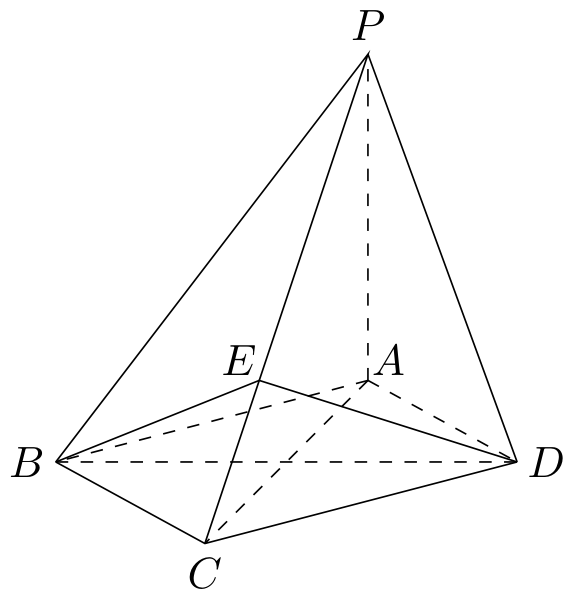
\includegraphics[width=7.1cm]{GaoKao/images/2012/syllabus_science/q18_fig1.png}
\end{center}

        \item 乒乓球比赛规则规定：一局比赛，双方比分在\(10\)平前，一方连续发球\(2\)次后，对方再连续发球\(2\)次，依次轮换. 每次发球，胜方得\(1\)分，负方得\(0\)分. 设在甲，乙的比赛中，每次发球，发球方得\(1\)分的概率为\(0.6\)，各次发球的胜负结果相互独立. 甲，乙的一局比赛中，甲先发球.
\begin{enumerate}
\item 求开始第\(4\)次发球时，甲，乙的比分为\(1\)比\(2\)的概率；
\item \( \xi \) 表示开始第 4 次发球时乙的得分，求 \( \xi \) 的期望.
\end{enumerate}

        \item 设函数 \(f(x) = ax + \cos x\)，\(x \in [0, \pi]\)：
\begin{enumerate}
\item 讨论 \( f(x) \) 的单调性；
\item 设 \( f(x) \leqslant 1 + \sin x \)，求 \( a \) 的取值范围.
\end{enumerate}

        \item 已知抛物线 \(C: y = (x + 1)^2\) 与圆 \(M: (x - 1)^2 + \left(y - \frac{1}{2}\right)^2 = r^2 \) （\(r > 0\)）有一个公共点 \(A\)，且在 \(A\) 处两曲线的切线为同一直线 \(l\).
\begin{enumerate}
\item 求 \(r\)；
\item 设 \(m\)，\(n\) 是异于 \(l\) 且与 \(C\) 及 \(M\) 都相切的两条直线，\(m\)，\(n\) 的交点为 \(D\)，求 \(D\) 到 \(l\) 的距离.
\end{enumerate}

        \item 函数 \( f(x) = x^2 - 2x - 3 \). 定义数列 \( \{x_n\} \) 如下： \(x_1 = 2\)，\(x_{n+1}\) 是过两点 \(P(4,5)\)，\(Q_n(x_n, f(x_n))\) 的直线 \( PQ_n \) 与 \( x \) 轴交点的横坐标.
\begin{enumerate}
\item 证明： \(2 \leqslant x_{n} < x_{n+1} < 3\).
\item 求数列 \(\{x_{n}\}\) 的通项公式.
\end{enumerate}

    \end{enumerate}

\end{description}


\subsection{2012年大纲卷（文）}\label{gk:2012年大纲卷（文）}

\begin{description}

    \item[一、选择题]

    \begin{enumerate}[leftmargin=5pt]

        \item 已知集合 \(A = \{x \mid x\text{ 是平行四边形}\}\)，\(B = \{x \mid x\text{ 是矩形}\}\)，\(C = \{x \mid x\text{ 是正方形}\}\)，\(D = \{x \mid x\text{ 是菱形}\}\)，则（\quad）

        {\centering\begin{tabular*}{\linewidth}{@{}@{\extracolsep{\fill}}llll@{}}
          \text{A. }\(A \subseteq B\)  &  \text{B. }\(C \subseteq B\)  &  \text{C. }\(D \subseteq C\)  &  \text{D. }\(A \subseteq D\)
        \end{tabular*}\par}

        \item 函数 \( y = \sqrt{x + 1} \) （\(x \geqslant -1\)）的反函数为（\quad）

        {\centering\begin{tabular*}{\linewidth}{@{}@{\extracolsep{\fill}}llll@{}}
          \text{A. }\( y = x^{2} - 1 \)（\(x \geqslant 0\)）  &  \text{B. }\( y = x^{2} - 1 \)（\(x \geqslant 1\)）  &  \text{C. }\( y = x^{2} + 1 \)（\(x \geqslant 0\)）  &  \text{D. }\( y = x^{2} + 1 \)（\(x \geqslant 1\)）
        \end{tabular*}\par}

        \item 若函数 \( f(x) = \sin \frac{x + \varphi}{3} \)（\(\varphi \in [0, 2\pi]\)）是偶函数，则 \( \varphi = \)（\quad）

        {\centering\begin{tabular*}{\linewidth}{@{}@{\extracolsep{\fill}}llll@{}}
          \text{A. }\(\frac{\pi}{2}\)  &  \text{B. }\(\frac{2\pi}{3}\)  &  \text{C. }\(\frac{3\pi}{2}\)  &  \text{D. }\(\frac{5\pi}{3}\)
        \end{tabular*}\par}

        \item 已知 \(\alpha\) 为第二象限角，\(\sin \alpha = \frac{3}{5}\)，则 \(\sin 2\alpha =\)（\quad）

        {\centering\begin{tabular*}{\linewidth}{@{}@{\extracolsep{\fill}}llll@{}}
          \text{A. }\(-\frac{24}{25}\)  &  \text{B. }\(-\frac{12}{25}\)  &  \text{C. }\(\frac{12}{25}\)  &  \text{D. }\(\frac{24}{25}\)
        \end{tabular*}\par}

        \item 椭圆的中心在原点，焦距为 \(4\)，一条准线为 \(x = -4\)，则该椭圆的方程为（\quad）

        {\centering\begin{tabular*}{\linewidth}{@{}@{\extracolsep{\fill}}llll@{}}
          \text{A. }\(\frac{x^2}{16} +\frac{y^2}{12} = 1\)  &  \text{B. }\(\frac{x^2}{12} +\frac{y^2}{8} = 1\)  &  \text{C. }\(\frac{x^2}{8} +\frac{y^2}{4} = 1\)  &  \text{D. }\(\frac{x^2}{12} +\frac{y^2}{4} = 1\)
        \end{tabular*}\par}

        \item 已知数列 \(\{a_{n}\}\) 的前 \(n\) 项和为 \(S_{n}\)，\(a_{1} = 1\)，\(S_{n} = 2a_{n+1}\)，则 \(S_{n} =\)（\quad）

        {\centering\begin{tabular*}{\linewidth}{@{}@{\extracolsep{\fill}}llll@{}}
          \text{A. }\(2^{n - 1}\)  &  \text{B. }\(\left(\frac{3}{2}\right)^{n - 1}\)  &  \text{C. }\(\left(\frac{2}{3}\right)^{n - 1}\)  &  \text{D. }\(\frac{1}{2^{n - 1}}\)
        \end{tabular*}\par}

        \item \(6\) 位选手依次演讲，其中选手甲不在第一个也不在最后一个演讲，则不同的演讲次序共有（\quad）

        {\centering\begin{tabular*}{\linewidth}{@{}@{\extracolsep{\fill}}llll@{}}
          \text{A. }\(240\) 种  &  \text{B. }\(360\) 种  &  \text{C. }\(480\) 种  &  \text{D. }\(720\) 种
        \end{tabular*}\par}

        \item 已知正四棱柱 \(ABCD - A_{1}B_{1}C_{1}D_{1}\) 中，\(AB = 2\)，\(CC_{1} = 2\sqrt{2}\)，\(E\) 为 \(CC_{1}\) 的中点，则直线 \(AC_{1}\) 到平面 \(BED\) 的距离为（\quad）

        {\centering\begin{tabular*}{\linewidth}{@{}@{\extracolsep{\fill}}llll@{}}
          \text{A. }2  &  \text{B. }\(\sqrt{3}\)  &  \text{C. }\(\sqrt{2}\)  &  \text{D. }1
        \end{tabular*}\par}

        \item \(\triangle ABC\) 中，\(AB\) 边的高为 \(CD\)，若 \(\overrightarrow{CB} = \bm{a}\)，\(\overrightarrow{CA} = \bm{b}\)，\(\bm{a} \cdot \bm{b} = 0\)，\(|\bm{a}| = 1\)，\(|\bm{b}| = 2\)，则 \(\overrightarrow{AD} =\)（\quad）

        {\centering\begin{tabular*}{\linewidth}{@{}@{\extracolsep{\fill}}llll@{}}
          \text{A. }\(\frac{1}{3}\bm{a} - \frac{1}{3}\bm{b}\)  &  \text{B. }\(\frac{2}{3}\bm{a} - \frac{2}{3}\bm{b}\)  &  \text{C. }\(\frac{3}{5}\bm{a} - \frac{3}{5}\bm{b}\)  &  \text{D. }\(\frac{4}{5}\bm{a} - \frac{4}{5}\bm{b}\)
        \end{tabular*}\par}

        \item 已知 \(F_{1}\)，\(F_{2}\) 为双曲线 \(C: x^{2} - y^{2} = 2\) 的左、右焦点，点 \(P\) 在 \(C\) 上，\(|PF_{1}| = 2|PF_{2}|\)，则 \(\cos \angle F_{1}PF_{2} =\)（\quad）

        {\centering\begin{tabular*}{\linewidth}{@{}@{\extracolsep{\fill}}llll@{}}
          \text{A. }\(\frac{1}{4}\)  &  \text{B. }\(\frac{3}{5}\)  &  \text{C. }\(\frac{3}{4}\)  &  \text{D. }\(\frac{4}{5}\)
        \end{tabular*}\par}

        \item 已知 \(x = \ln \pi\)，\(y = \log_5 2\)，\(z = {\mathrm{e}}^{-\frac{1}{2}}\)，则（\quad）

        {\centering\begin{tabular*}{\linewidth}{@{}@{\extracolsep{\fill}}llll@{}}
          \text{A. }\(x < y < z\)  &  \text{B. }\(z < x < y\)  &  \text{C. }\(z < y < x\)  &  \text{D. }\(y < z < x\)
        \end{tabular*}\par}

        \item 正方形 \(ABCD\) 的边长为 \(1\)，点 \(E\) 在边 \(AB\) 上，点 \(F\) 在边 \(BC\) 上，\(AE = BF = \frac{1}{3}\). 动点 \(P\) 从 \(E\) 出发沿直线向 \(F\) 运动，每当碰到正方形的边时反弹，反弹时反射角等于入射角，当点 \(P\) 第一次碰到 \(E\) 时，\(P\) 与正方形的边碰撞的次数为（\quad）

        {\centering\begin{tabular*}{\linewidth}{@{}@{\extracolsep{\fill}}llll@{}}
          \text{A. }8  &  \text{B. }6  &  \text{C. }4  &  \text{D. }3
        \end{tabular*}\par}

    \end{enumerate}

\end{description}

\begin{description}

    \item[二、填空题]

    \begin{enumerate}[leftmargin=5pt]

      \addtocounter{enumi}{+12}

        \item \(\left(x + \frac{1}{2x}\right)^8\) 的展开式中 \(x^2\) 的系数为\rule[-0.3ex]{3em}{0.4pt}.

        \item 若 \(x\)，\(y\) 满足约束条件 \(\begin{cases}
x - y + 1 \geqslant 0,\\
x + y - 3 \leqslant 0,\\
x + 3y - 3 \geqslant 0,
\end{cases}\) 则 \(z = 3x - y\) 的最小值为\rule[-0.3ex]{3em}{0.4pt}.

        \item 当函数 \( y = \sin x - \sqrt{3}\cos x \)（\(0 \leqslant x < 2\pi\)）取得最大值时，\( x = \)\rule[-0.3ex]{3em}{0.4pt}.

        \item 已知正方体 \(ABCD - A_{1}B_{1}C_{1}D_{1}\) 中，\(E\)，\(F\) 分别为 \(BB_{1}\)，\(CC_{1}\) 的中点，那么异面直线 \(AE\) 与 \(D_{1}F\) 所成角的余弦值为\rule[-0.3ex]{3em}{0.4pt}.

    \end{enumerate}

\end{description}

\begin{description}

    \item[三、解答题]

    \begin{enumerate}[leftmargin=5pt]

      \addtocounter{enumi}{+16}

        \item \(\triangle ABC\) 的内角 \(A\)，\(B\)，\(C\) 成等差数列，其对边 \(a\)，\(b\)，\(c\) 满足 \(2b^{2} = 3ac\)，求 \(A\).

        \item 已知数列 \( \{a_{n}\} \) 中， \( a_{1}=1 \)，前 \(n\) 项和 \( S_{n}=\frac{n+2}{3}a_{n} \).
\begin{enumerate}
\item 求 \(a_{2}\)，\(a_{3}\).
\item 求 \( \{a_{n}\} \) 的通项公式.
\end{enumerate}

        \item 如图，四棱锥 \(P - ABCD\) 中，底面 \(ABCD\) 为菱形，\(PA \perp\) 底面 \(ABCD\)，\(AC = 2\sqrt{2}\)，\(PA = 2\)，\(E\) 是 \(PC\) 上的一点，\(PE = 2EC\).
\begin{enumerate}
\item 证明：\(PC \perp\) 平面 \(BED\).
\item 设二面角 \(A - PB - C\) 为 \(90^{\circ}\)，求 \(PD\) 与平面 \(PBC\) 所成角的大小.
\end{enumerate}
\begin{center}
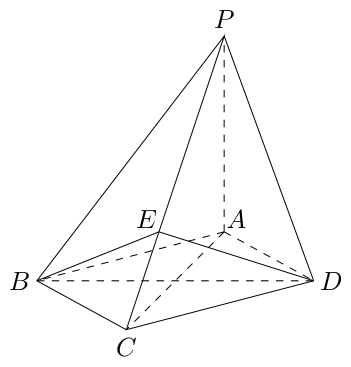
\includegraphics[width=7.3cm]{GaoKao/images/2012/syllabus_liberal/q19_fig1.png}
\end{center}

        \item 乒乓球比赛规则规定：一局比赛，双方比分在\(10\)平前，一方连续发球\(2\)次后，对方再连续发球\(2\)次，依次轮换. 每次发球，胜方得\(1\)分，负方得\(0\)分. 设在甲，乙的比赛中，每次发球，发球方得\(1\)分的概率为\(0.6\)，各次发球的胜负结果相互独立. 甲，乙的一局比赛中，甲先发球.
\begin{enumerate}
\item 求开始第 \(4\) 次发球时，甲，乙的比分为 \(1\) 比 \(2\) 的概率.
\item 求开始第 \(5\) 次发球时，甲得分领先的概率.
\end{enumerate}

        \item 已知函数 \( f(x) = \frac{1}{3} x^3 + x^2 + ax \).
\begin{enumerate}
\item 讨论 \( f(x) \) 的单调性.
\item 设 \( f(x) \) 有两个极值点 \(x_{1}\)，\(x_{2}\)，若过两点 \((x_{1}, f(x_{1}))\)，\((x_{2}, f(x_{2}))\) 的直线 \( l \) 与 \( x \) 轴的交点在曲线 \( f(x) \) 上，求 \( a \) 的值.
\end{enumerate}

    \end{enumerate}

\end{description}

\begin{description}

    \item[四、选考题]

    \begin{enumerate}[leftmargin=5pt]

      \addtocounter{enumi}{+21}

        \item \textbf{【选修4-1：几何证明选讲】}

已知抛物线 \(C: y = (x + 1)^2\) 与圆 \(M: (x - 1)^2 + (y - \frac{1}{2})^2 = r^2\)（\(r > 0\)）有一个公共点 \(A\)，且在 \(A\) 处两曲线的切线为同一直线 \(l\).
\begin{enumerate}
\item 求 \(r\).
\item 设 \(m\)，\(n\) 是异于 \(l\) 且与 \(C\) 及 \(M\) 都相切的两条直线，\(m\)，\(n\) 的交点为 \(D\)，求 \(D\) 到 \(l\) 的距离.
\end{enumerate}

    \end{enumerate}

\end{description}


\subsection{2012年全国卷（理）}\label{gk:2012年全国卷（理）}

\begin{description}

    \item[一、选择题]

    \begin{enumerate}[leftmargin=5pt]

        \item 已知集合 \(A = \{1, 2, 3, 4, 5\}\)，\(B = \{(x, y) \mid x \in A, y \in A, x - y \in A\}\)，则 \(B\) 中所含元素的个数为（\quad）

        {\centering\begin{tabular*}{\linewidth}{@{}@{\extracolsep{\fill}}llll@{}}
          \text{A. }3  &  \text{B. }6  &  \text{C. }8  &  \text{D. }10
        \end{tabular*}\par}

        \item 将 \(2\) 名教师，\(4\) 名学生分成 \(2\) 个小组，分别安排到甲，乙两地参加社会实践活动，每个小组由 \(1\) 名教师和 \(2\) 名学生组成，不同的安排方案共有（\quad）

        {\centering\begin{tabular*}{\linewidth}{@{}@{\extracolsep{\fill}}llll@{}}
          \text{A. }\(12\text{ 种}\)  &  \text{B. }\(10\text{ 种}\)  &  \text{C. }\(9\text{ 种}\)  &  \text{D. }\(8\text{ 种}\)
        \end{tabular*}\par}

        \item 下面是关于复数 \(z = \frac{2}{-1 + \i}\) 的四个命题：\(p_1: |z| = 2\)，\(p_2: z^2 = 2\i\)；\(p_3: z\) 的共轭复数为 \(1 + \i\)；\(p_4: z\) 的虚部为 \(-1\). 其中的真命题为（\quad）

        {\centering\begin{tabular*}{\linewidth}{@{}@{\extracolsep{\fill}}llll@{}}
          \text{A. }\(p_{2}\)，\(p_{3}\)  &  \text{B. }\(p_{1}\)，\(p_{2}\)  &  \text{C. }\(p_{2}\)，\(p_{4}\)  &  \text{D. }\(p_{3}\)，\(p_{4}\)
        \end{tabular*}\par}

        \item 设 \(F_{1}\)，\(F_{2}\) 是椭圆 \(E: \frac{x^{2}}{a^{2}} + \frac{y^{2}}{b^{2}} = 1\)（\(a > b > 0\)）的左，右焦点，\(P\) 为直线 \(x = \frac{3a}{2}\) 上一点，\(\triangle F_{2}PF_{1}\) 是底角为 \(30^{\circ}\) 的等腰三角形，则 \(E\) 的离心率为（\quad）

        {\centering\begin{tabular*}{\linewidth}{@{}@{\extracolsep{\fill}}llll@{}}
          \text{A. }\( \frac{1}{2} \)  &  \text{B. }\( \frac{2}{3} \)  &  \text{C. }\( \frac{3}{4} \)  &  \text{D. }\( \frac{4}{5} \)
        \end{tabular*}\par}

        \item 已知 \(\{a_{n}\}\) 为等比数列，\(a_{4} + a_{7} = 2\)，\(a_{5}a_{6} = -8\)，则 \(a_{1} + a_{10} =\)（\quad）

        {\centering\begin{tabular*}{\linewidth}{@{}@{\extracolsep{\fill}}llll@{}}
          \text{A. }7  &  \text{B. }5  &  \text{C. }\(-5\)  &  \text{D. }\(-7\)
        \end{tabular*}\par}

        \item 如果执行下面的程序框图，输入正整数 \(N\)（\(N \geqslant 2\)）和实数 \(a_{1}\)，\(a_{2}\)，\(\cdots\)，\(a_{N}\)，输出 \(A\)，\(B\)，则（\quad）

\begin{center}
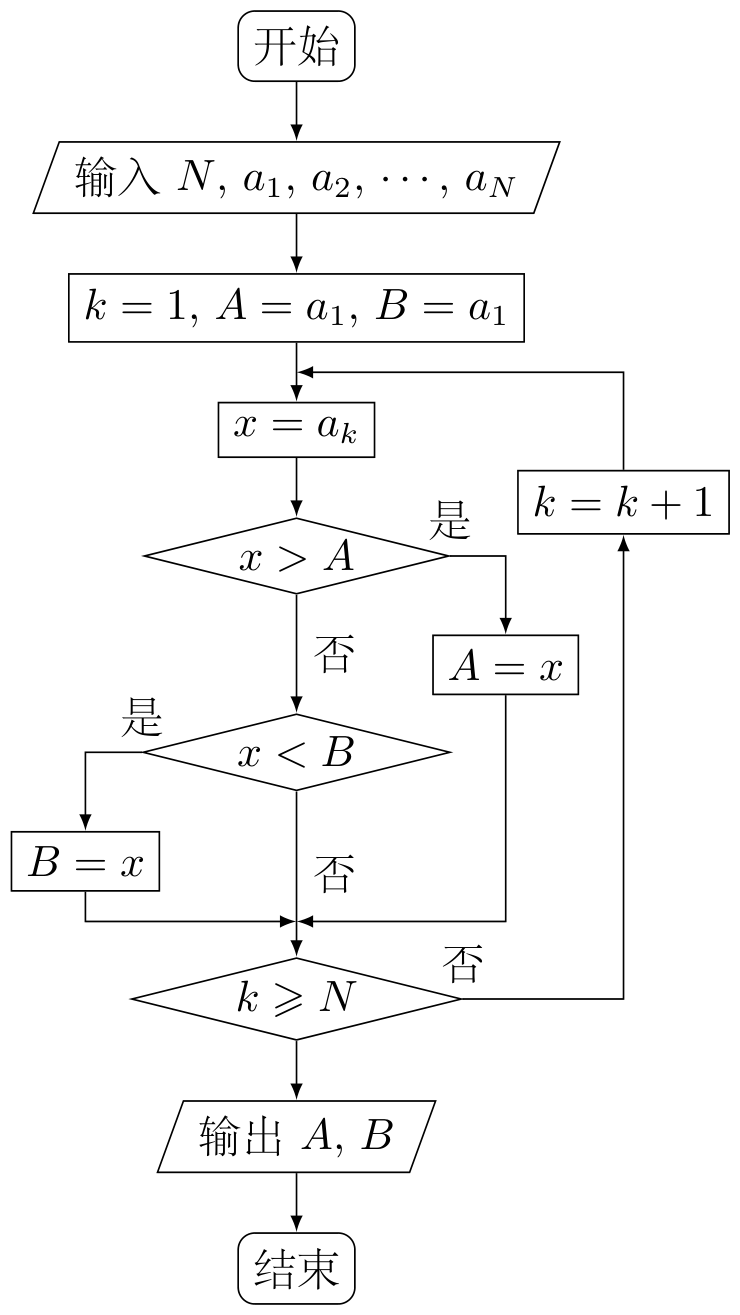
\includegraphics[width=4.3cm]{GaoKao/images/2012/new_curriculum_science/q6_fig1.png}
\end{center}

        {\centering\begin{tabular*}{\linewidth}{@{}@{\extracolsep{\fill}}llll@{}}
          \text{A. }\(A + B\) 为 \(a_{1}\)，\(a_{2}\)，\(\cdots\)，\(a_{N}\) 的和  &  \text{B. }\(\frac{A + B}{2}\) 为 \(a_1\)，\(a_2\)，\(\dots\)，\(a_N\) 的算术平均数  &  \text{C. }\(A\) 和 \(B\) 分别是 \(a_{1}\)，\(a_{2}\)，\(\dots\)，\(a_{N}\) 中最大的数和最小的数  &  \text{D. }\(A\) 和 \(B\) 分别是 \(a_{1}\)，\(a_{2}\)，\(\dots\)，\(a_{N}\) 中最小的数和最大的数
        \end{tabular*}\par}

        \item 如图，网格上小正方形的边长为 \(1\)，粗线画出的是某几何体的三视图，则此几何体的体积为（\quad）

\begin{center}
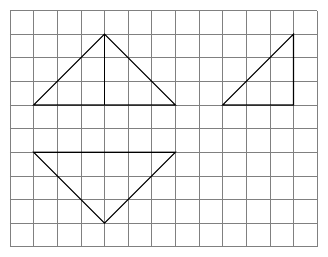
\includegraphics[width=6.1cm]{GaoKao/images/2012/new_curriculum_science/q7_fig1.png}
\end{center}

        {\centering\begin{tabular*}{\linewidth}{@{}@{\extracolsep{\fill}}llll@{}}
          \text{A. }6  &  \text{B. }9  &  \text{C. }12  &  \text{D. }18
        \end{tabular*}\par}

        \item 等轴双曲线 \(C\) 的中心在原点，焦点在 \(x\) 轴上，\(C\) 与抛物线 \( y^{2} = 16x \) 的准线交于 \(A\)，\(B\) 两点，\( |AB| = 4\sqrt{3} \)，则 \(C\) 的实轴长为（\quad）

        {\centering\begin{tabular*}{\linewidth}{@{}@{\extracolsep{\fill}}llll@{}}
          \text{A. }\(\sqrt{2}\)  &  \text{B. }\(2\sqrt{2}\)  &  \text{C. }4  &  \text{D. }8
        \end{tabular*}\par}

        \item 已知 \(\omega > 0\)，函数 \(f(x) = \sin \left(\omega x + \frac{\pi}{4}\right)\) 在 \(\left(\frac{\pi}{2}, \pi\right)\) 单调递减，则 \(\omega\) 的取值范围是（\quad）

        {\centering\begin{tabular*}{\linewidth}{@{}@{\extracolsep{\fill}}llll@{}}
          \text{A. }\(\left[\frac{1}{2}, \frac{5}{4}\right]\)  &  \text{B. }\(\left[\frac{1}{2}, \frac{3}{4}\right]\)  &  \text{C. }\(\left(0, \frac{1}{2}\right]\)  &  \text{D. }\((0, 2]\)
        \end{tabular*}\par}

        \item 已知函数 \( f(x) = \frac{1}{\ln (x + 1) - x} \)，则 \( y = f(x) \) 的图象大致为（\quad）

        {\centering\begin{tabular*}{\linewidth}{@{}@{\extracolsep{\fill}}cccc@{}}
          \text{A. }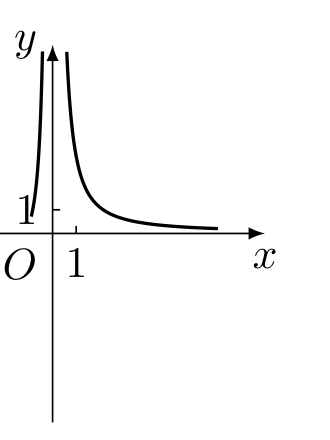
\includegraphics[width=0.15\paperwidth]{GaoKao/images/2012/new_curriculum_science/q10_optA.png}  &  \text{B. }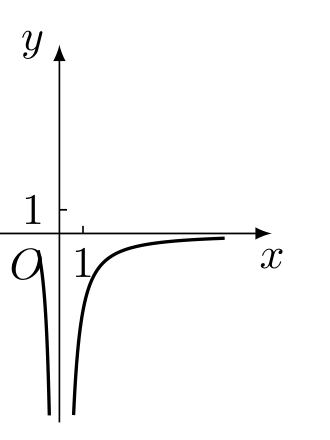
\includegraphics[width=0.15\paperwidth]{GaoKao/images/2012/new_curriculum_science/q10_optB.png}  &  \text{C. }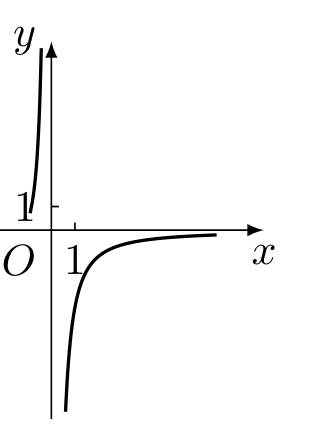
\includegraphics[width=0.15\paperwidth]{GaoKao/images/2012/new_curriculum_science/q10_optC.png}  &  \text{D. }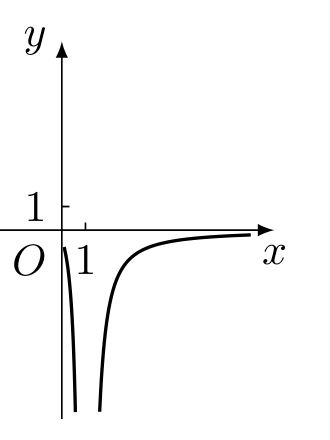
\includegraphics[width=0.15\paperwidth]{GaoKao/images/2012/new_curriculum_science/q10_optD.png}
        \end{tabular*}\par}

        \item 已知三棱锥 \(S - ABC\) 的所有顶点都在球 \(O\) 的球面上，\(\triangle ABC\) 是边长为 \(1\) 的正三角形，\(SC\) 为球 \(O\) 的直径，且 \(SC = 2\)，则此棱锥的体积为（\quad）

        {\centering\begin{tabular*}{\linewidth}{@{}@{\extracolsep{\fill}}llll@{}}
          \text{A. }\(\frac{\sqrt{2}}{6}\)  &  \text{B. }\( \frac{\sqrt{3}}{6} \)  &  \text{C. }\( \frac{\sqrt{2}}{3} \)  &  \text{D. }\( \frac{\sqrt{2}}{2} \)
        \end{tabular*}\par}

        \item 设点 \(P\) 在曲线 \(y = \frac{1}{2} {\mathrm{e}}^{x}\) 上，点 \(Q\) 在曲线 \(y = \ln (2x)\) 上，则 \(|PQ|\) 的最小值为（\quad）

        {\centering\begin{tabular*}{\linewidth}{@{}@{\extracolsep{\fill}}llll@{}}
          \text{A. }\(1 - \ln 2\)  &  \text{B. }\(\sqrt{2}\,(1 - \ln 2)\)  &  \text{C. }\(1 + \ln 2\)  &  \text{D. }\(\sqrt{2}\,(1 + \ln 2)\)
        \end{tabular*}\par}

    \end{enumerate}

\end{description}

\begin{description}

    \item[二、填空题]

    \begin{enumerate}[leftmargin=5pt]

      \addtocounter{enumi}{+12}

        \item 已知向量 \(\bm{a}\)，\(\bm{b}\) 夹角为 \(45^{\circ}\)，且 \(|\bm{a}| = 1\)，\(|2\bm{a} - \bm{b}| = \sqrt{10}\)，则 \(|\bm{b}| =\rule[-0.3ex]{3em}{0.4pt}\).

        \item 设 \(x\)，\(y\) 满足约束条件 \(\begin{cases}
x - y \geqslant -1,\\
x + y \leqslant 3,\\
x \geqslant 0,\\
y \geqslant 0,
\end{cases}\) 则 \(z = x - 2y\) 的取值范围为\rule[-0.3ex]{3em}{0.4pt}.

        \item 某一部件由三个电子元件按下图方式连接而成，元件 \(1\) 或元件 \(2\) 正常工作，且元件 \(3\) 正常工作，则部件正常工作. 设三个电子元件的使用寿命（单位：小时）均服从正态分布 \(N(1000, 50^{2})\)，且各个元件能否正常工作相互独立，那么该部件的使用寿命超过 \(1000\) 小时的概率为\rule[-0.3ex]{3em}{0.4pt}.

\begin{center}
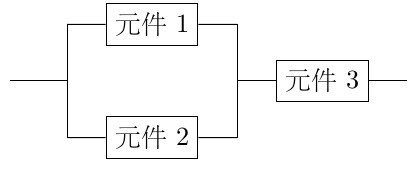
\includegraphics[width=6.9cm]{GaoKao/images/2012/new_curriculum_science/q15_fig1.png}
\end{center}

        \item 数列 \(\{a_{n}\}\) 满足 \(a_{n + 1} + (-1)^n a_n = 2n - 1\)，则 \(\{a_n\}\) 的前 \(60\) 项和为\rule[-0.3ex]{3em}{0.4pt}.

    \end{enumerate}

\end{description}

\begin{description}

    \item[三、解答题]

    \begin{enumerate}[leftmargin=5pt]

      \addtocounter{enumi}{+16}

        \item 已知 \(a\)，\(b\)，\(c\) 分别为 \(\triangle ABC\) 三个内角 \(A\)，\(B\)，\(C\) 的对边，\(a \cos C + \sqrt{3} a \sin C - b - c = 0\).

\begin{enumerate}
\item 求 \(A\)；
\item 若 \(a = 2\)，\(\triangle ABC\) 的面积为 \(\sqrt{3}\)，求 \(b\)，\(c\).
\end{enumerate}

        \item 某花店每天以每枝 \(5\) 元的价格从农场购进若干枝玫瑰花，然后以每枝 \(10\) 元的价格出售，如果当天卖不完，剩下的玫瑰花作垃圾处理.

\begin{enumerate}
\item 若花店一天购进 \(16\) 枝玫瑰花，求当天的利润 \(y\)（单位：元）关于当天需求量 \(n\)（单位：枝，\(n \in \mathbb{N}\)）的函数解析式；
\item 花店记录了 \(100\) 天玫瑰花的日需求量（单位：枝），整理得下表：

\begin{center}
\renewcommand{\arraystretch}{1.2}
\begin{tabular}{|c|c|c|c|c|c|c|c|}
\hline
日需求量 \(n\) & \(14\) & \(15\) & \(16\) & \(17\) & \(18\) & \(19\) & \(20\) \\
\hline
频数 & \(10\) & \(20\) & \(16\) & \(16\) & \(15\) & \(13\) & \(10\) \\
\hline
\end{tabular}
\end{center}

以 \(100\) 天记录的各需求量的频率作为各需求量发生的概率.

\begin{enumerate}
\item 若花店一天购进 \(16\) 枝玫瑰花，\(X\) 表示当天的利润（单位：元），求 \(X\) 的分布列，数学期望及方差；
\item 若花店计划一天购进 \(16\) 枝或 \(17\) 枝玫瑰花，你认为应购进 \(16\) 枝还是 \(17\) 枝？请说明理由.
\end{enumerate}
\end{enumerate}

        \item 如图，直三棱柱 \(ABC - A_{1}B_{1}C_{1}\) 中，\(AC = BC = \frac{1}{2} AA_{1}\)，\(D\) 是棱 \(AA_{1}\) 的中点，\(DC_{1} \perp BD\).

\begin{enumerate}
\item 证明：\(DC_{1} \perp BC\)；
\item 求二面角 \(A_{1} - BD - C_{1}\) 的大小.
\end{enumerate}
\begin{center}
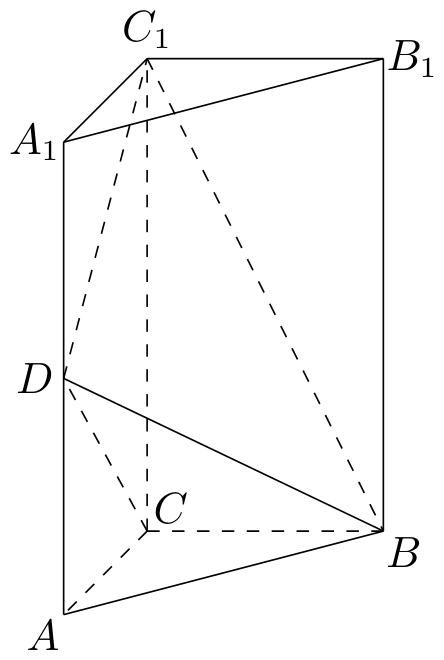
\includegraphics[width=4.6cm]{GaoKao/images/2012/new_curriculum_science/q19_fig1.png}
\end{center}

        \item 设抛物线 \(C: x^{2} = 2py\)（\(p > 0\)）的焦点为 \(F\)，准线为 \(l\)，\(A\) 为 \(C\) 上一点，已知以 \(F\) 为圆心，\(FA\) 为半径的圆 \(F\) 交 \(l\) 于 \(B\)，\(D\) 两点.

\begin{enumerate}
\item 若 \(\angle BFD = 90^{\circ}\)，\(\triangle ABD\) 的面积为 \(4\sqrt{2}\)，求 \(p\) 的值及圆 \(F\) 的方程；
\item 若 \(A\)，\(B\)，\(F\) 三点在同一直线 \(m\) 上，直线 \(n\) 与 \(m\) 平行，且 \(n\) 与 \(C\) 只有一个公共点，求坐标原点到 \(m\)，\(n\) 距离的比值.
\end{enumerate}

        \item 已知函数 \(f(x)\) 满足 \(f(x) = f'(1){\mathrm{e}}^{x-1} - f(0)x + \frac{1}{2}x^2\).

\begin{enumerate}
\item 求 \(f(x)\) 的解析式及单调区间；
\item 若 \(f(x) \geqslant \frac{1}{2}x^2 + ax + b\)，求 \((a + 1)b\) 的最大值.
\end{enumerate}

    \end{enumerate}

\end{description}

\begin{description}

    \item[四、选考题]

    \begin{enumerate}[leftmargin=5pt]

      \addtocounter{enumi}{+21}

        \item \textbf{【选修4-1：几何证明选讲】}

如图，\(D\)，\(E\) 分别为 \(\triangle ABC\) 边 \(AB\)，\(AC\) 的中点，直线 \(DE\) 交 \(\triangle ABC\) 的外接圆于 \(F\)，\(G\) 两点. 若 \(CF \parallel AB\)，证明：

\begin{enumerate}
\item \(CD = BC\)；
\item \(\triangle BCD \sim \triangle GBD\).
\end{enumerate}
\begin{center}
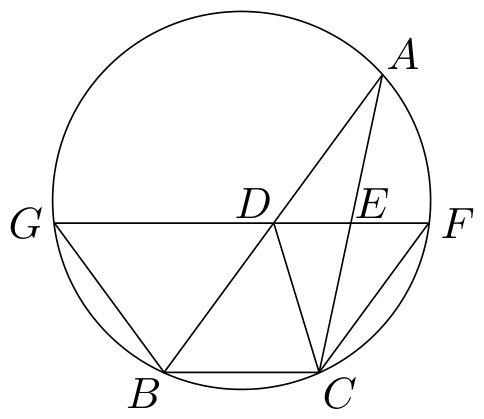
\includegraphics[width=6.0cm]{GaoKao/images/2012/new_curriculum_science/q22_fig1.png}
\end{center}

        \item \textbf{【选修4-4：坐标系与参数方程】}

已知曲线 \(C_1\) 的参数方程是 \(\begin{cases}
x = 2\cos \varphi,\\
y = 3\sin \varphi,
\end{cases}\) （\(\varphi\) 是参数）以坐标原点为极点，\(x\) 轴的非负半轴为极轴建立极坐标系，曲线 \(C_2\) 的极坐标方程是 \(\rho = 2\)，正方形 \(ABCD\) 的顶点都在 \(C_2\) 上，且 \(A\)，\(B\)，\(C\)，\(D\) 依逆时针次序排列，点 \(A\) 的极坐标为 \(\left(2, \frac{\pi}{3}\right)\).

\begin{enumerate}
\item 求点 \(A\)，\(B\)，\(C\)，\(D\) 的直角坐标；
\item 设 \(P\) 为 \(C_1\) 上任意一点，求 \(|PA|^2 + |PB|^2 + |PC|^2 + |PD|^2\) 的取值范围.
\end{enumerate}

        \item \textbf{【选修4-5：不等式选讲】}

已知函数 \( f(x) = |x + a| + |x - 2| \).

\begin{enumerate}
\item 当 \(a = -3\) 时，求不等式 \(f(x) \geqslant 3\) 的解集；
\item 若 \( f(x) \leqslant |x - 4| \) 的解集包含 \([1, 2]\)，求 \( a \) 的取值范围.
\end{enumerate}

    \end{enumerate}

\end{description}


\subsection{2012年全国卷（文）}\label{gk:2012年全国卷（文）}

\begin{description}

    \item[一、选择题]

    \begin{enumerate}[leftmargin=5pt]

        \item 已知集合 \(A = \{x \mid x^2 - x - 2 < 0\}\)，\(B = \{x \mid -1 < x < 1\}\)，则（\quad）

        {\centering\begin{tabular*}{\linewidth}{@{}@{\extracolsep{\fill}}llll@{}}
          \text{A. }\(A \subsetneq B\)  &  \text{B. }\(B \subsetneq A\)  &  \text{C. }\(A = B\)  &  \text{D. }\(A \cap B = \varnothing\)
        \end{tabular*}\par}

        \item 复数 \(z = \frac{-3 + \i}{2 + \i}\) 的共轭复数是（\quad）

        {\centering\begin{tabular*}{\linewidth}{@{}@{\extracolsep{\fill}}llll@{}}
          \text{A. }\(2 + \i\)  &  \text{B. }\(2 - \i\)  &  \text{C. }\(-1 + \i\)  &  \text{D. }\(-1 - \i\)
        \end{tabular*}\par}

        \item 在一组样本数据 \((x_{1}, y_{1})\)，\((x_{2}, y_{2})\)，\(\cdots\)，\((x_{n}, y_{n})\)（\(n \geqslant 2\)，\(x_{1}\)，\(x_{2}\)，\(\cdots\)，\(x_{n}\) 不全相等）的散点图中，若所有样本点 \((x_{i}, y_{i})\)（\(i = 1, 2, \cdots, n\)）都在直线 \(y = \frac{1}{2}x + 1\) 上，则这组样本数据的样本相关系数为（\quad）

        {\centering\begin{tabular*}{\linewidth}{@{}@{\extracolsep{\fill}}llll@{}}
          \text{A. }\(-1\)  &  \text{B. }\(0\)  &  \text{C. }\( \frac{1}{2} \)  &  \text{D. }\(1\)
        \end{tabular*}\par}

        \item 设 \(F_{1}\)，\(F_{2}\) 是椭圆 \(E: \frac{x^{2}}{a^{2}} + \frac{y^{2}}{b^{2}} = 1\)（\(a > b > 0\)）的左，右焦点，\(P\) 为直线 \(x = \frac{3a}{2}\) 上一点，\(\triangle F_{2}PF_{1}\) 是底角为 \(30^{\circ}\) 的等腰三角形，则 \(E\) 的离心率为（\quad）

        {\centering\begin{tabular*}{\linewidth}{@{}@{\extracolsep{\fill}}llll@{}}
          \text{A. }\( \frac{1}{2} \)  &  \text{B. }\( \frac{2}{3} \)  &  \text{C. }\( \frac{3}{4} \)  &  \text{D. }\( \frac{4}{5} \)
        \end{tabular*}\par}

        \item 已知正三角形 \(ABC\) 的顶点 \(A(1,1)\)，\(B(1,3)\)，顶点 \(C\) 在第一象限，若点 \((x,y)\) 在 \(\triangle ABC\) 内部，则 \(z = -x + y\) 的取值范围是（\quad）

        {\centering\begin{tabular*}{\linewidth}{@{}@{\extracolsep{\fill}}llll@{}}
          \text{A. }\( (1-\sqrt{3},2) \)  &  \text{B. }\((0,2)\)  &  \text{C. }\((\sqrt{3} - 1, 2)\)  &  \text{D. }\((0, 1 + \sqrt{3})\)
        \end{tabular*}\par}

        \item 如果执行下面的程序框图，输入正整数 \(N\)（\(N \geqslant 2\)）和实数 \(a_{1}\)，\(a_{2}\)，\(\cdots\)，\(a_{N}\)，输出 \(A\)，\(B\)，则（\quad）

\begin{center}
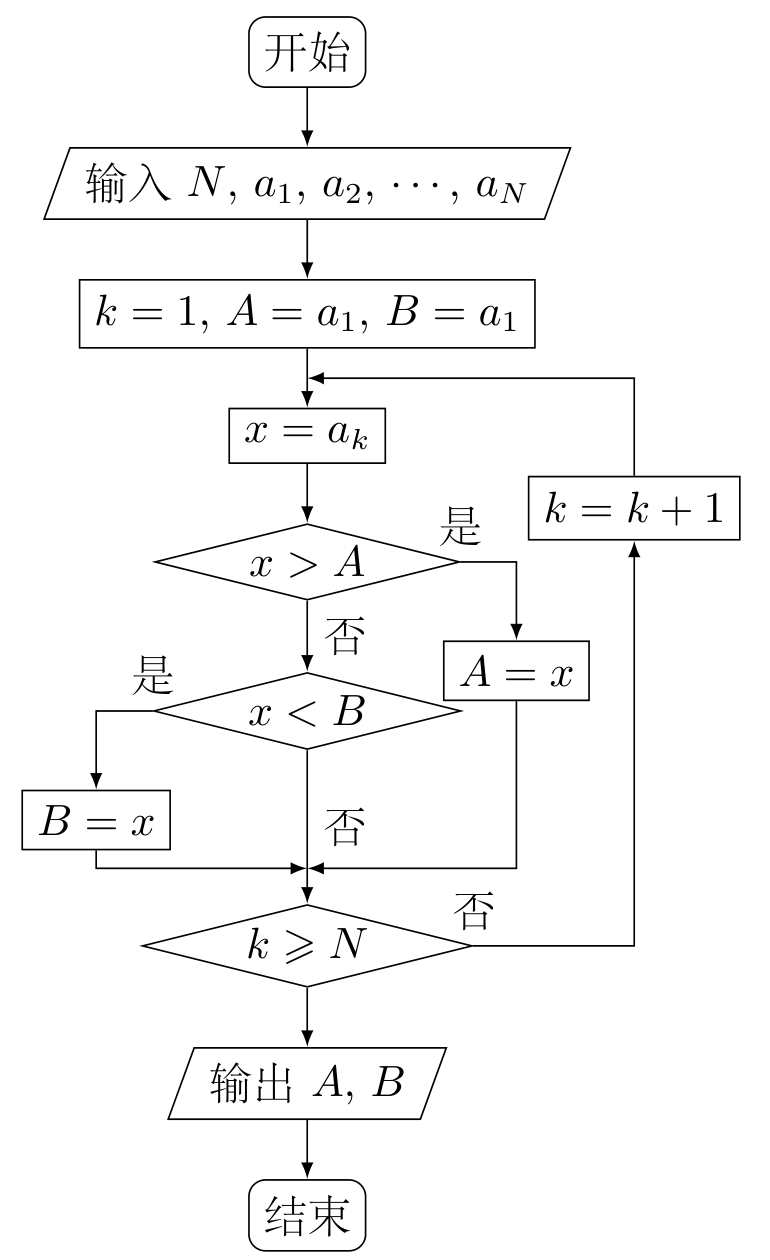
\includegraphics[width=0.66\linewidth]{GaoKao/images/2012/new_curriculum_liberal/q6_fig1.png}
\end{center}

        {\centering\begin{tabular*}{\linewidth}{@{}@{\extracolsep{\fill}}llll@{}}
          \text{A. }\(A+B\) 为 \(a_1\)，\(a_2\)，\(\dots\)，\(a_N\) 的和  &  \text{B. }\(\frac{A+B}{2}\) 为 \(a_1\)，\(a_2\)，\(\dots\)，\(a_N\) 的算术平均数  &  \text{C. }\(A\) 和 \(B\) 分别是 \(a_1\)，\(a_2\)，\(\dots\)，\(a_N\) 中最大的数和最小的数  &  \text{D. }\(A\) 和 \(B\) 分别是 \(a_1\)，\(a_2\)，\(\dots\)，\(a_N\) 中最小的数和最大的数
        \end{tabular*}\par}

        \item 如图，网格上小正方形的边长为 \(1\)，粗线画出的是某几何体的三视图，则此几何体的体积为（\quad）

\begin{center}
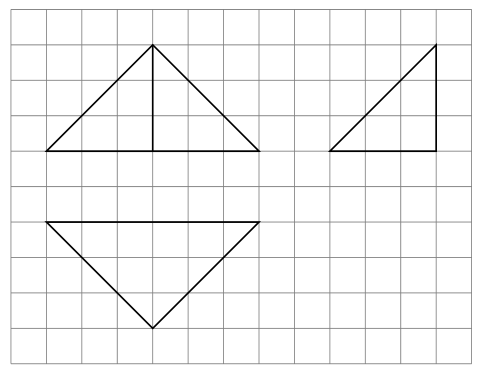
\includegraphics[width=5.6cm]{GaoKao/images/2012/new_curriculum_liberal/q7_fig1.png}
\end{center}

        {\centering\begin{tabular*}{\linewidth}{@{}@{\extracolsep{\fill}}llll@{}}
          \text{A. }\(6\)  &  \text{B. }\(9\)  &  \text{C. }\(12\)  &  \text{D. }\(18\)
        \end{tabular*}\par}

        \item 平面 \(\alpha\) 截球 \(O\) 的球面所得圆的半径为 \(1\)，球心 \(O\) 到平面 \(\alpha\) 的距离为 \(\sqrt{2}\)，则此球的体积为（\quad）

        {\centering\begin{tabular*}{\linewidth}{@{}@{\extracolsep{\fill}}llll@{}}
          \text{A. }\(\sqrt{6}\pi\)  &  \text{B. }\(4\sqrt{3}\pi\)  &  \text{C. }\(4\sqrt{6}\pi\)  &  \text{D. }\(6\sqrt{3}\pi\)
        \end{tabular*}\par}

        \item 已知 \(\omega > 0\)，\(0 < \varphi < \pi\)，直线 \(x = \frac{\pi}{4}\) 和 \(x = \frac{5\pi}{4}\) 是函数 \(f(x) = \sin (\omega x + \varphi)\) 图象的两条相邻的对称轴，则 \(\varphi =\)（\quad）

        {\centering\begin{tabular*}{\linewidth}{@{}@{\extracolsep{\fill}}llll@{}}
          \text{A. }\( \frac{\pi}{4} \)  &  \text{B. }\( \frac{\pi}{3} \)  &  \text{C. }\( \frac{\pi}{2} \)  &  \text{D. }\( \frac{3\pi}{4} \)
        \end{tabular*}\par}

        \item 等轴双曲线 \(C\) 的中心在原点，焦点在 \(x\) 轴上，\(C\) 与抛物线 \(y^{2} = 16x\) 的准线交于 \(A\)，\(B\) 两点，\(|AB| = 4\sqrt{3}\)，则 \(C\) 的实轴长为（\quad）

        {\centering\begin{tabular*}{\linewidth}{@{}@{\extracolsep{\fill}}llll@{}}
          \text{A. }\(\sqrt{2}\)  &  \text{B. }\(2\sqrt{2}\)  &  \text{C. }\(4\)  &  \text{D. }\(8\)
        \end{tabular*}\par}

        \item 当 \(0 < x \leqslant \frac{1}{2}\) 时，\(4^x < \log_a x\)，则 \(a\) 的取值范围是（\quad）

        {\centering\begin{tabular*}{\linewidth}{@{}@{\extracolsep{\fill}}llll@{}}
          \text{A. }\(\left(0, \frac{\sqrt{2}}{2}\right)\)  &  \text{B. }\(\left(\frac{\sqrt{2}}{2}, 1\right)\)  &  \text{C. }\((1, \sqrt{2})\)  &  \text{D. }\((\sqrt{2}, 2)\)
        \end{tabular*}\par}

        \item 数列 \(\{a_{n}\}\) 满足 \(a_{n + 1} + (-1)^{n}a_{n} = 2n - 1\)，则 \(\{a_{n}\}\) 的前 \(60\) 项和为（\quad）

        {\centering\begin{tabular*}{\linewidth}{@{}@{\extracolsep{\fill}}llll@{}}
          \text{A. }\(3690\)  &  \text{B. }\(3660\)  &  \text{C. }\(1845\)  &  \text{D. }\(1830\)
        \end{tabular*}\par}

    \end{enumerate}

\end{description}

\begin{description}

    \item[二、填空题]

    \begin{enumerate}[leftmargin=5pt]

      \addtocounter{enumi}{+12}

        \item 曲线 \(y = x(3\ln x + 1)\) 在点 \((1,1)\) 处的切线方程为\rule[-0.3ex]{3em}{0.4pt}.

        \item 等比数列 \(\{a_{n}\}\) 的前 \(n\) 项和为 \(S_{n}\)，若 \(S_{3} + 3S_{2} = 0\)，则公比 \(q = \)\rule[-0.3ex]{3em}{0.4pt}.

        \item 已知向量 \(\bm{a}\)，\(\bm{b}\) 夹角为 \(45^{\circ}\)，且 \(|\bm{a}| = 1\)，\(|2\bm{a} - \bm{b}| = \sqrt{10}\)，则 \(|\bm{b}| = \)\rule[-0.3ex]{3em}{0.4pt}.

        \item 设函数 \( f(x) = \frac{(x + 1)^2 + \sin x}{x^2 + 1} \) 的最大值为 \(M\)，最小值为 \( m \)，则 \( M + m = \)\rule[-0.3ex]{3em}{0.4pt}.

    \end{enumerate}

\end{description}

\begin{description}

    \item[三、解答题]

    \begin{enumerate}[leftmargin=5pt]

      \addtocounter{enumi}{+16}

        \item 已知 \(a\)，\(b\)，\(c\) 分别为 \(\triangle ABC\) 三个内角 \(A\)，\(B\)，\(C\) 的对边，\(a \cos C + \sqrt{3} a \sin C - b - c = 0\).

\begin{enumerate}
\item 求 \(A\)；
\item 若 \(a = 2\)，\(\triangle ABC\) 的面积为 \(\sqrt{3}\)，求 \(b\)，\(c\).
\end{enumerate}

        \item 某花店每天以每枝 \(5\) 元的价格从农场购进若干枝玫瑰花，然后以每枝 \(10\) 元的价格出售，如果当天卖不完，剩下的玫瑰花作垃圾处理.

\begin{enumerate}
\item 若花店一天购进 \(17\) 枝玫瑰花，当天的利润 \(y\)（单位：元）关于当天需求量 \(n\)（单位：枝，\(n \in \mathbb{N}\)）的函数解析式；
\item 花店记录了 \(100\) 天玫瑰花的需求量（单位：枝），整理得下表：

\begin{center}
\renewcommand{\arraystretch}{1.2}
\begin{tabular}{|c|c|c|c|c|c|c|c|}
\hline
日需求量 \(n\) & \(14\) & \(15\) & \(16\) & \(17\) & \(18\) & \(19\) & \(20\) \\
\hline
频数 & \(10\) & \(20\) & \(16\) & \(16\) & \(15\) & \(13\) & \(10\) \\
\hline
\end{tabular}
\end{center}

以 \(100\) 天记录的各需求量的频率作为各需求量发生的概率.

\begin{enumerate}
\item 假设花店在这 \(100\) 天内每天购进 \(17\) 枝玫瑰花，求这 \(100\) 天的日利润（单位：元）的平均数；
\item 若花店一天购进 \(17\) 枝玫瑰花，以 \(100\) 天记录的各需求量的频率作为各需求量发生的概率，求当天的利润不少于 \(75\) 元的概率.
\end{enumerate}
\end{enumerate}

        \item 如图，三棱柱 \(ABC - A_{1}B_{1}C_{1}\) 中，侧棱垂直底面，\(\angle ACB = 90^{\circ}\)，\(AC = BC = \frac{1}{2} AA_{1}\)，\(D\) 是棱 \(AA_{1}\) 的中点.

\begin{enumerate}
\item 证明：平面 \(BDC_{1} \perp\) 平面 \(BDC\)；
\item 平面 \(BDC_{1}\) 分此棱柱为两部分，求这两部分体积的比.
\end{enumerate}

\begin{center}
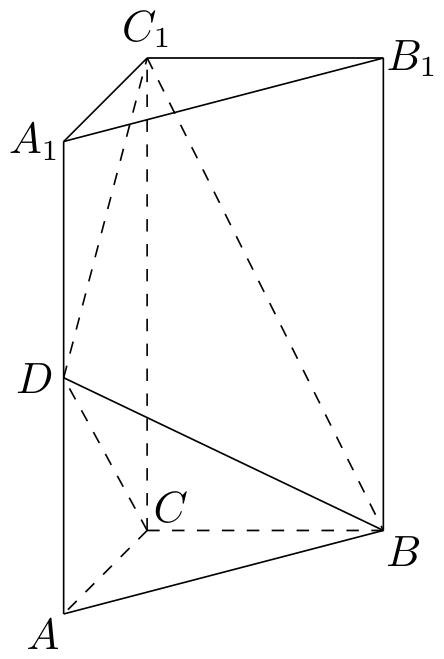
\includegraphics[width=4.6cm]{GaoKao/images/2012/new_curriculum_liberal/q19_fig1.png}
\end{center}

        \item 设抛物线 \(C: x^{2} = 2py\)（\(p > 0\)）的焦点为 \(F\)，准线为 \(l\)，\(A\) 为 \(C\) 上一点，已知以 \(F\) 为圆心，\(FA\) 为半径的圆 \(F\) 交 \(l\) 于 \(B\)，\(D\) 两点.

\begin{enumerate}
\item 若 \(\angle BFD = 90^{\circ}\)，\(\triangle ABD\) 的面积为 \(4\sqrt{2}\)，求 \(p\) 的值及圆 \(F\) 的方程；
\item 若 \(A\)，\(B\)，\(F\) 三点在同一直线 \(m\) 上，直线 \(n\) 与 \(m\) 平行，且 \(n\) 与 \(C\) 只有一个公共点，求坐标原点到 \(m\)，\(n\) 距离的比值.
\end{enumerate}

        \item 设函数 \( f(x) = {\mathrm{e}}^{x} - ax - 2 \).

\begin{enumerate}
\item 求 \( f(x) \) 的单调区间；
\item 若 \(a = 1\)，\(k\) 为整数，且当 \(x > 0\) 时，\((x-k)f'(x) + x + 1 > 0\)，求 \(k\) 的最大值.
\end{enumerate}

        \item 如图，\(D\)，\(E\) 分别为 \(\triangle ABC\) 边 \(AB\)，\(AC\) 的中点，直线 \(DE\) 交 \(\triangle ABC\) 的外接圆于 \(F\)，\(G\) 两点. 若 \(CF\parallel AB\)，证明：

\begin{enumerate}
\item \(CD = BC\)；
\item \(\triangle BCD \sim \triangle GBD\).
\end{enumerate}

\begin{center}
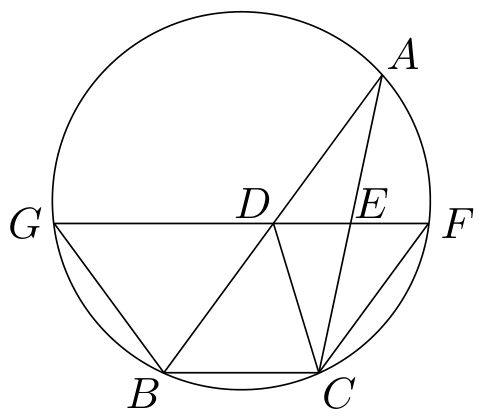
\includegraphics[width=3.6cm]{GaoKao/images/2012/new_curriculum_liberal/q22_fig1.png}
\end{center}

        \item 已知曲线 \(C_1\) 的参数方程是 \(\begin{cases}
x = 2\cos \varphi,\\
y = 3\sin \varphi,
\end{cases}\) （\(\varphi\) 是参数）以坐标原点为极点，\(x\) 轴的非负半轴为极轴建立极坐标系，曲线 \(C_2\) 的极坐标方程是 \(\rho = 2\)，正方形 \(ABCD\) 的顶点都在 \(C_2\) 上，且 \(A\)，\(B\)，\(C\)，\(D\) 依逆时针次序排列，点 \(A\) 的极坐标为 \(\left(2, \frac{\pi}{3}\right)\).

\begin{enumerate}
\item 求点 \(A\)，\(B\)，\(C\)，\(D\) 的直角坐标；
\item 设 \(P\) 为 \(C_{1}\) 上任意一点，求 \(|PA|^{2} + |PB|^{2} + |PC|^{2} + |PD|^{2}\) 的取值范围.
\end{enumerate}

        \item 已知函数 \( f(x) = |x + a| + |x - 2| \).

\begin{enumerate}
\item 当 \(a = -3\) 时，求不等式 \( f(x) \geqslant 3 \) 的解集；
\item 若 \(f(x) \leqslant |x - 4|\) 的解集包含 \([1,2]\)，求 \(a\) 的取值范围.
\end{enumerate}

    \end{enumerate}

\end{description}


\subsection{2012年安徽卷（理）}\label{gk:2012年安徽卷（理）}

\begin{description}

    \item[一、选择题]

    \begin{enumerate}[leftmargin=5pt]

        \item 复数 \(z\) 满足 \((z - \i)(2 - \i) = 5\)，则 \(z =\)（\quad）

        {\centering\begin{tabular*}{\linewidth}{@{}@{\extracolsep{\fill}}llll@{}}
          \text{A. }\(-2 - 2\i\)  &  \text{B. }\(-2 + 2\i\)  &  \text{C. }\(2 - 2\i\)  &  \text{D. }\(2 + 2\i\)
        \end{tabular*}\par}

        \item 下列函数中，不满足 \( f(2x) = 2f(x) \) 的是（\quad）

        {\centering\begin{tabular*}{\linewidth}{@{}@{\extracolsep{\fill}}llll@{}}
          \text{A. }\(f(x) = |x|\)  &  \text{B. }\(f(x) = x - |x|\)  &  \text{C. }\(f(x) = x + 1\)  &  \text{D. }\(f(x) = -x\)
        \end{tabular*}\par}

        \item 如图所示，程序框图（算法流程图）的输出结果是（\quad）

\begin{center}
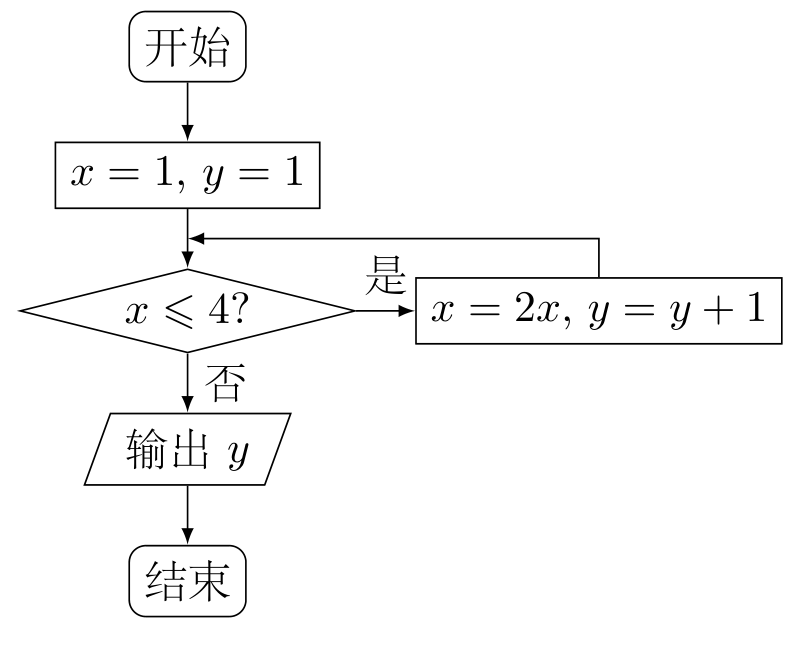
\includegraphics[width=6.5cm]{GaoKao/images/2012/anhui_science/q3_fig1.png}
\end{center}

        {\centering\begin{tabular*}{\linewidth}{@{}@{\extracolsep{\fill}}llll@{}}
          \text{A. }3  &  \text{B. }4  &  \text{C. }5  &  \text{D. }8
        \end{tabular*}\par}

        \item 公比为 \(\sqrt[3]{2}\) 的等比数列 \(\{a_{n}\}\) 的各项都是正数，且 \(a_{3}a_{11} = 16\)，则 \(\log_2a_{16} =\)（\quad）

        {\centering\begin{tabular*}{\linewidth}{@{}@{\extracolsep{\fill}}llll@{}}
          \text{A. }4  &  \text{B. }5  &  \text{C. }6  &  \text{D. }7
        \end{tabular*}\par}

        \item 甲，乙两人在一次射击比赛中各射靶 \(5\) 次，两人成绩的条形统计图如图所示，则（\quad）

\begin{center}
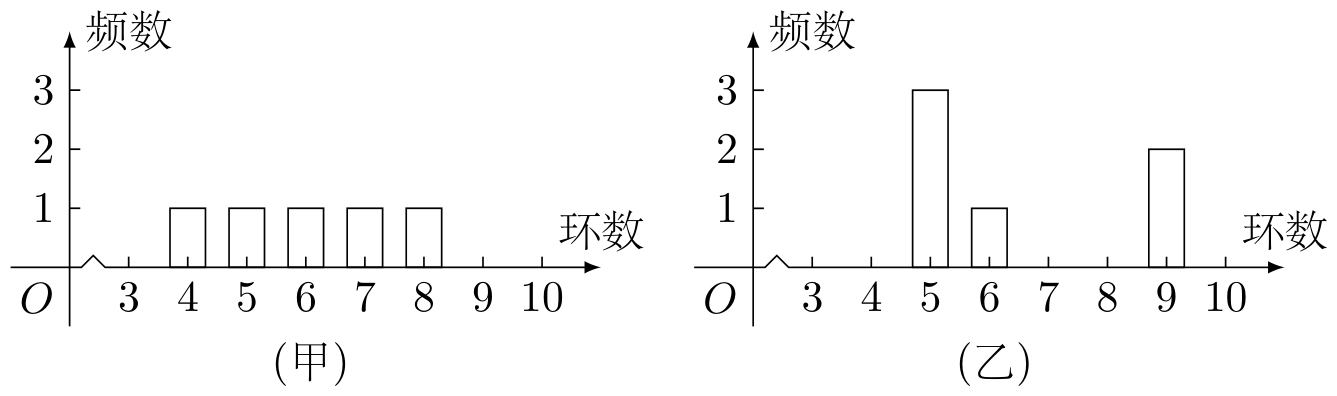
\includegraphics[width=13.0cm]{GaoKao/images/2012/anhui_science/q5_fig1.png}
\end{center}

        {\centering\begin{tabular*}{\linewidth}{@{}@{\extracolsep{\fill}}llll@{}}
          \text{A. }甲的成绩的平均数小于乙的成绩的平均数  &  \text{B. }甲的成绩的中位数等于乙的成绩的中位数  &  \text{C. }甲的成绩的方差小于乙的成绩的方差  &  \text{D. }甲的成绩的极差小于乙的成绩的极差
        \end{tabular*}\par}

        \item 设平面 \(\alpha\) 与平面 \(\beta\) 相交于直线 \(m\)，直线 \(a\) 在平面 \(\alpha\) 内，直线 \(b\) 在平面 \(\beta\) 内，且 \(b \perp m\)，则 “\(\alpha \perp \beta\)” 是 “\(a \perp b\)” 的（\quad）

        {\centering\begin{tabular*}{\linewidth}{@{}@{\extracolsep{\fill}}llll@{}}
          \text{A. }充分不必要条件  &  \text{B. }必要不充分条件  &  \text{C. }充分必要条件  &  \text{D. }既不充分也不必要条件
        \end{tabular*}\par}

        \item \((x^{2} + 2)\left(\frac{1}{x^{2}} -1\right)^{5}\) 的展开式的常数项是（\quad）

        {\centering\begin{tabular*}{\linewidth}{@{}@{\extracolsep{\fill}}llll@{}}
          \text{A. }\(-3\)  &  \text{B. }\(-2\)  &  \text{C. }2  &  \text{D. }3
        \end{tabular*}\par}

        \item 在平面直角坐标系中，点 \(O(0,0)\)，\(P(6,8)\)，将向量 \(\overrightarrow{OP}\) 绕点 \(O\) 按逆时针方向旋转 \(\frac{3\pi}{4}\) 后得向量 \(\overrightarrow{OQ}\)，则点 \(Q\) 的坐标是（\quad）

        {\centering\begin{tabular*}{\linewidth}{@{}@{\extracolsep{\fill}}llll@{}}
          \text{A. }\((-7\sqrt{2}, - \sqrt{2})\)  &  \text{B. }\((-7\sqrt{2}, \sqrt{2})\)  &  \text{C. }\((-4\sqrt{6}, - 2)\)  &  \text{D. }\((-4\sqrt{6}, 2)\)
        \end{tabular*}\par}

        \item 过抛物线 \( y^{2} = 4x \) 的焦点 \(F\) 的直线交该抛物线于 \(A\)，\(B\) 两点，\(O\) 为坐标原点，若 \( |AF| = 3 \)，则 \( \triangle AOB \) 的面积为（\quad）

        {\centering\begin{tabular*}{\linewidth}{@{}@{\extracolsep{\fill}}llll@{}}
          \text{A. }\(\frac{\sqrt{2}}{2}\)  &  \text{B. }\(\sqrt{2}\)  &  \text{C. }\(\frac{3\sqrt{2}}{2}\)  &  \text{D. }\(2 \sqrt{2}\)
        \end{tabular*}\par}

        \item 6位同学在毕业聚会活动中进行纪念品的交换，任意两位同学之间最多交换一次，进行交换的两位同学互赠一份纪念品. 已知6位同学之间共进行了13次交换，则收到4份纪念品的同学人数为（\quad）

        {\centering\begin{tabular*}{\linewidth}{@{}@{\extracolsep{\fill}}llll@{}}
          \text{A. }1 或 3  &  \text{B. }1 或 4  &  \text{C. }2 或 3  &  \text{D. }2 或 4
        \end{tabular*}\par}

    \end{enumerate}

\end{description}

\begin{description}

    \item[二、填空题]

    \begin{enumerate}[leftmargin=5pt]

      \addtocounter{enumi}{+10}

        \item 若 \(x\)，\(y\) 满足约束条件 \(\begin{cases}
x \geqslant 0,\\
x + 2y \geqslant 3,\\
2x + y \leqslant 3,
\end{cases}\) 则 \(x - y\) 的取值范围是\rule[-0.3ex]{3em}{0.4pt}.

        \item 某几何体的三视图如图所示，该几何体的表面积是\rule[-0.3ex]{3em}{0.4pt}.

\begin{center}
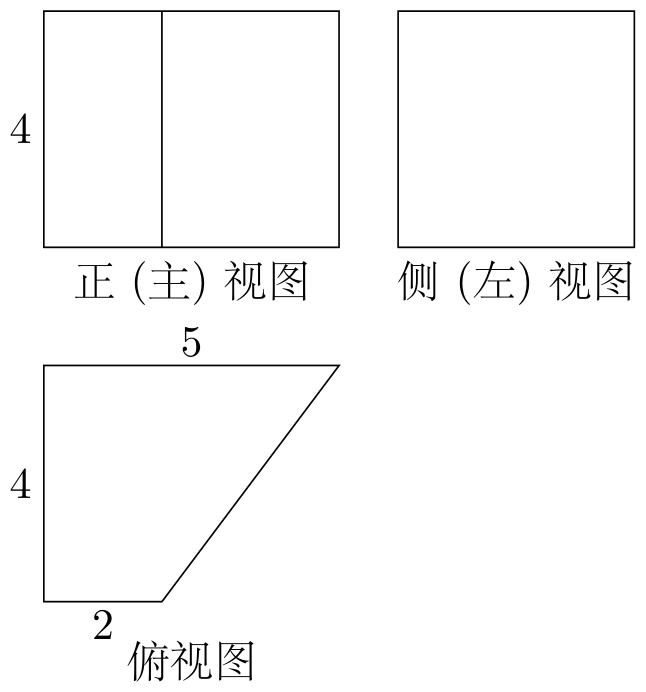
\includegraphics[width=6.3cm]{GaoKao/images/2012/anhui_science/q12_fig1.png}
\end{center}

        \item 在极坐标系中，圆 \(\rho = 4\sin \theta\) 的圆心到直线 \(\theta = \frac{\pi}{6}\)（\(\rho \in \mathbb{R}\)）的距离是\rule[-0.3ex]{3em}{0.4pt}.

        \item 若平面向量 \(\bm{a}\)，\(\bm{b}\) 满足 \(|2\bm{a} - \bm{b}| \leqslant 3\)，则 \(\bm{a} \cdot \bm{b}\) 的最小值是\rule[-0.3ex]{3em}{0.4pt}.

        \item 设 \(\triangle ABC\) 的内角 \(A\)，\(B\)，\(C\) 所对边的长分别为 \(a\)，\(b\)，\(c\)，则下列命题正确的是\rule[-0.3ex]{3em}{0.4pt}. （写出所有正确命题的编号）

\begin{enumerate}
\item 若 \(ab > c^2\)，则 \(C < \frac{\pi}{3}\).
\item 若 \(a + b > 2c\)，则 \(C < \frac{\pi}{3}\).
\item 若 \(a^3 + b^3 = c^3\)，则 \(C < \frac{\pi}{2}\).
\item 若 \((a + b)c < 2ab\)，则 \(C > \frac{\pi}{2}\).
\item 若 \((a^2 + b^2)c^2 < 2a^2b^2\)，则 \(C > \frac{\pi}{3}\).
\end{enumerate}

    \end{enumerate}

\end{description}

\begin{description}

    \item[三、解答题]

    \begin{enumerate}[leftmargin=5pt]

      \addtocounter{enumi}{+15}

        \item 设函数 \( f(x) = \frac{\sqrt{2}}{2}\cos \left(2x + \frac{\pi}{4}\right) + \sin^2 x. \)

\begin{enumerate}
\item 求 \( f(x) \) 的最小正周期.
\item 设函数 \( g(x) \) 对任意 \( x \in \mathbb{R} \)，有 \( g\left(x + \frac{\pi}{2}\right) = g(x) \)，且当 \( x \in \left[0, \frac{\pi}{2}\right] \) 时，\( g(x) = \frac{1}{2} - f(x) \). 求 \( g(x) \) 在区间 \([- \pi, 0]\) 上的解析式.
\end{enumerate}

        \item 某单位招聘面试，每次从试题库中随机调用一道试题，若调用的是 A 类型试题，则使用后该试题回库，并增补一道 A 类型试题和一道 B 类型试题入库，此次调题工作结束；若调用的是 B 类型试题，则使用后该试题回库，此次调题工作结束. 试题库中现共有 \( n + m \) 道试题，其中有 \(n\) 道 A 类型试题和 \(m\) 道 B 类型试题，以 \(X\) 表示两次调题工作完成后，试题库中 A 类试题的数量.

\begin{enumerate}
\item 求 \(X = n + 2\) 的概率.
\item 设 \(m = n\)，求 \(X\) 的分布列和均值 （数学期望）.
\end{enumerate}

        \item 平面图形 \(ABB_{1}A_{1}C_{1}C\) 如图1所示，其中 \(BB_{1}C_{1}C\) 是矩形，\(BC = 2\)，\(BB_{1} = 4\)，\(AB = AC = \sqrt{2}\)，\(A_{1}B_{1} = A_{1}C_{1} = \sqrt{5}\). 现将该平面图形分别沿 \(BC\) 和 \(B_{1}C_{1}\) 折叠，使 \(\triangle ABC\) 与 \(\triangle A_{1}B_{1}C_{1}\) 所在平面都与平面 \(BB_{1}C_{1}C\) 垂直，再分别连接 \(A_{1}A\)，\(A_{1}B\)，\(A_{1}C_{1}\) 得到如图2所示的空间图形，对此空间图形解答下列问题.

\begin{enumerate}
\item 证明： \( AA_{1} \perp BC\).
\item 求 \(AA_{1}\) 的长.
\item 求二面角 \( A - BC - A_{1} \) 的余弦值.
\end{enumerate}

\begin{center}
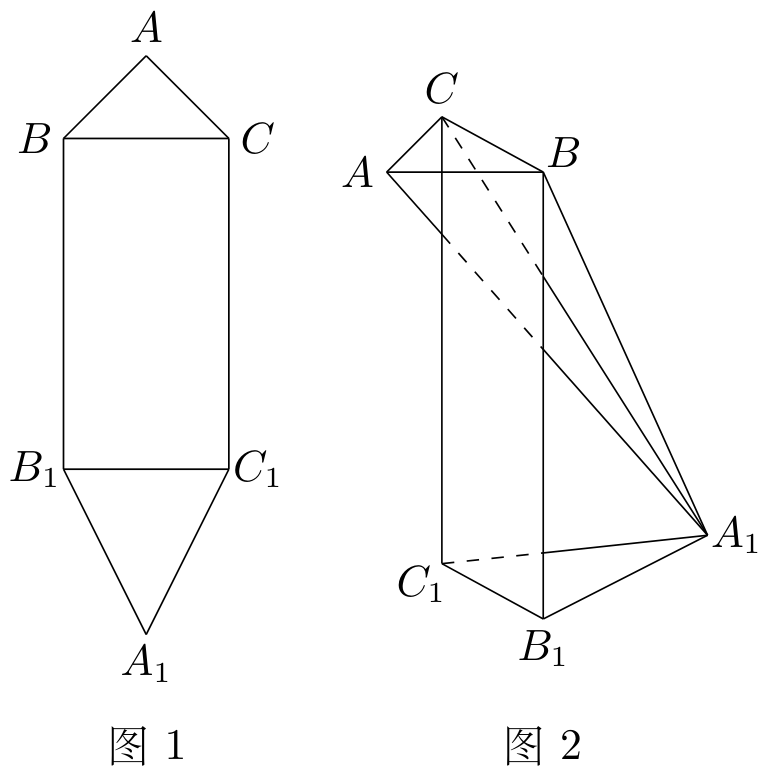
\includegraphics[width=7.2cm]{GaoKao/images/2012/anhui_science/q18_fig1.png}
\end{center}

        \item 设函数 \( f(x) = a{\mathrm{e}}^{x} + \frac{1}{a{\mathrm{e}}^{x}} + b  \) （\(a > 0\)）.

\begin{enumerate}
\item 求 \( f(x) \) 在 \( [0, +\infty) \) 内的最小值.
\item 设曲线 \( y = f(x) \) 在点 \( (2, f(2)) \) 处的切线方程为 \( y = \frac{3}{2} x \)，求 \(a\)，\(b\) 的值.
\end{enumerate}

        \item 如图，点 \(F_{1}(-c,0)\)，\(F_{2}(c,0)\) 分别是椭圆 \(C\)：\(\frac{x^{2}}{a^{2}} + \frac{y^{2}}{b^{2}} = 1\)（\(a > b > 0\)）的左，右焦点，过点 \(F_{1}\) 作 \(x\) 轴的垂线交椭圆 \(C\) 的上半部分于点 \(P\)，过点 \(F_{2}\) 作直线 \(PF_{2}\) 的垂线交直线 \(x = \frac{a^{2}}{c}\) 于点 \(Q\).

\begin{enumerate}
\item 如果点 \(Q\) 的坐标是 \((4,4)\)，求此时椭圆 \(C\) 的方程.
\item 证明：直线 \(PQ\) 与椭圆 \(C\) 只有一个交点.
\end{enumerate}

\begin{center}
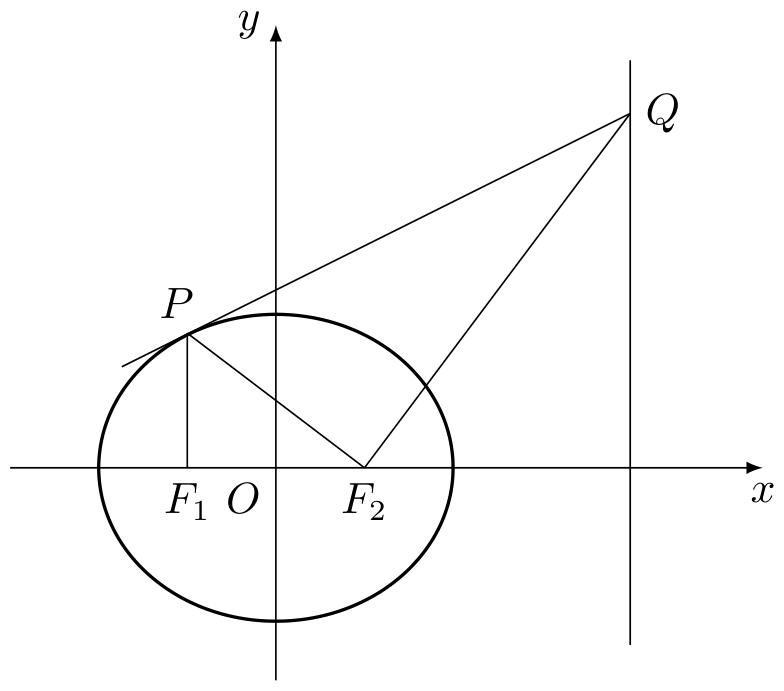
\includegraphics[width=7.9cm]{GaoKao/images/2012/anhui_science/q19_fig1.png}
\end{center}

        \item 数列 \(\{x_{n}\}\) 满足 \(x_{1} = 0\)，\(x_{n + 1} = -x_{n}^{2} + x_{n} + c \) （\(n \in \mathbf{N}^{*}\)）.

\begin{enumerate}
\item 证明： \(\{x_{n}\}\) 是递减数列的充分必要条件是 \(c < 0\).
\item 求 \(c\) 的取值范围，使 \( \{x_{n}\} \) 是递增数列.
\end{enumerate}

    \end{enumerate}

\end{description}


\subsection{2012年安徽卷（文）}\label{gk:2012年安徽卷（文）}

\begin{description}

    \item[一、选择题]

    \begin{enumerate}[leftmargin=5pt]

        \item 复数 \(z\) 满足 \((z - \i)\i = 2 + \i\)，则 \(z =\)（\quad）

        {\centering\begin{tabular*}{\linewidth}{@{}@{\extracolsep{\fill}}llll@{}}
          \text{A. }\(-1 - \i\)  &  \text{B. }\(1 - \i\)  &  \text{C. }\(-1 + 3\i\)  &  \text{D. }\(1 - 2\i\)
        \end{tabular*}\par}

        \item 设集合 \(A = \{x \mid -3 \leqslant 2x - 1 \leqslant 3\}\)，集合 \(B\) 为函数 \(y = \lg (x - 1)\) 的定义域，则 \(A \cap B =\)（\quad）

        {\centering\begin{tabular*}{\linewidth}{@{}@{\extracolsep{\fill}}llll@{}}
          \text{A. }\((1, 2)\)  &  \text{B. }\([1, 2]\)  &  \text{C. }\([1,2)\)  &  \text{D. }\((1,2]\)
        \end{tabular*}\par}

        \item \(\log_29\cdot \log_34 =\) （\quad）

        {\centering\begin{tabular*}{\linewidth}{@{}@{\extracolsep{\fill}}llll@{}}
          \text{A. }\(\frac{1}{4}\)  &  \text{B. }\(\frac{1}{2}\)  &  \text{C. }2  &  \text{D. }4
        \end{tabular*}\par}

        \item 命题“存在实数 \(x\)，使 \(x > 1\)”的否定是（\quad）

        {\centering\begin{tabular*}{\linewidth}{@{}@{\extracolsep{\fill}}llll@{}}
          \text{A. }对任意实数 \(x\)，都有 \(x > 1\)  &  \text{B. }不存在实数 \(x\)，使 \(x \leqslant 1\)  &  \text{C. }对任意实数 \(x\)，都有 \(x \leqslant 1\)  &  \text{D. }存在实数 \(x\)，使 \(x \leqslant 1\)
        \end{tabular*}\par}

        \item 公比为 2 的等比数列 \(\{a_{n}\}\) 的各项都是正数，且 \(a_{3}a_{11} = 16\)，则 \(a_{5} =\)（\quad）

        {\centering\begin{tabular*}{\linewidth}{@{}@{\extracolsep{\fill}}llll@{}}
          \text{A. }1  &  \text{B. }2  &  \text{C. }4  &  \text{D. }8
        \end{tabular*}\par}

        \item 如图所示，程序框图 （算法流程图） 的输出结果是（\quad）

\begin{center}
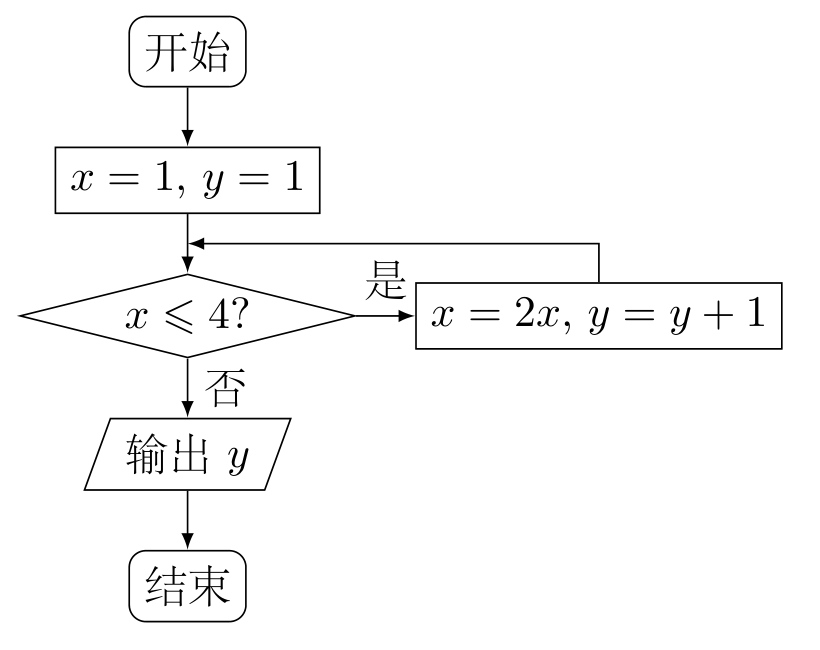
\includegraphics[width=0.70\linewidth]{GaoKao/images/2012/anhui_liberal/q6_fig1.png}
\end{center}

        {\centering\begin{tabular*}{\linewidth}{@{}@{\extracolsep{\fill}}llll@{}}
          \text{A. }3  &  \text{B. }4  &  \text{C. }5  &  \text{D. }8
        \end{tabular*}\par}

        \item 要得到函数 \( y = \cos (2x + 1) \) 的图象，只要将函数 \( y = \cos 2x \) 的图象（\quad）

        {\centering\begin{tabular*}{\linewidth}{@{}@{\extracolsep{\fill}}llll@{}}
          \text{A. }向左平移 1 个单位  &  \text{B. }向右平移 1 个单位  &  \text{C. }向左平移 \(\frac{1}{2}\) 个单位  &  \text{D. }向右平移 \(\frac{1}{2}\) 个单位
        \end{tabular*}\par}

        \item 若 \(x\)，\(y\) 满足约束条件 \(\begin{cases}
x \geqslant 0,\\
x + 2y \geqslant 3,\\
2x + y \leqslant 3,
\end{cases}\) 则 \(z = x - y\) 的最小值是（\quad）

        {\centering\begin{tabular*}{\linewidth}{@{}@{\extracolsep{\fill}}llll@{}}
          \text{A. }\(-3\)  &  \text{B. }0  &  \text{C. }\( \frac{3}{2} \)  &  \text{D. }3
        \end{tabular*}\par}

        \item 若直线 \(x - y + 1 = 0\) 与圆 \((x - a)^2 + y^2 = 2\) 有公共点，则实数 \(a\) 的取值范围是（\quad）

        {\centering\begin{tabular*}{\linewidth}{@{}@{\extracolsep{\fill}}llll@{}}
          \text{A. }\([-3, - 1]\)  &  \text{B. }\([-1, 3]\)  &  \text{C. }\([-3, 1]\)  &  \text{D. }\((- \infty, -3] \cup [1, +\infty)\)
        \end{tabular*}\par}

        \item 袋中共有 6 个除了颜色外完全相同的球，其中有 1 个红球，2 个白球和 3 个黑球. 从袋中任取两球，两球颜色为一白一黑的概率等于（\quad）

        {\centering\begin{tabular*}{\linewidth}{@{}@{\extracolsep{\fill}}llll@{}}
          \text{A. }\( \frac{1}{5} \)  &  \text{B. }\( \frac{2}{5} \)  &  \text{C. }\( \frac{3}{5} \)  &  \text{D. }\( \frac{4}{5} \)
        \end{tabular*}\par}

    \end{enumerate}

\end{description}

\begin{description}

    \item[二、填空题]

    \begin{enumerate}[leftmargin=5pt]

      \addtocounter{enumi}{+10}

        \item 设向量 \(\bm{a} = (1, 2m)\)，\(\bm{b} = (m + 1, 1)\)，\(\bm{c} = (2, m)\)，若 \((\bm{a} + \bm{c}) \perp \bm{b}\)，则 \(|\bm{a}| = \)\rule[-0.3ex]{3em}{0.4pt}.

        \item 某几何体的三视图如图所示，该几何体的体积是\rule[-0.3ex]{3em}{0.4pt}.

\begin{center}
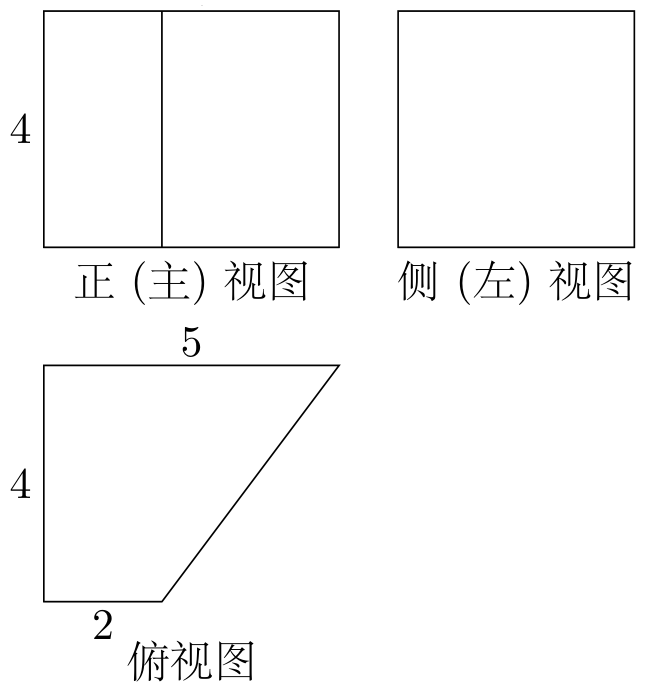
\includegraphics[width=6.3cm]{GaoKao/images/2012/anhui_liberal/q12_fig1.png}
\end{center}

        \item 若函数 \( f(x) = |2x + a| \) 的单调递增区间是 \([3, +\infty)\)，则 \( a = \)\rule[-0.3ex]{3em}{0.4pt}.

        \item 过抛物线 \( y^{2}=4x \) 的焦点 \(F\) 的直线交该抛物线于 \(A, B\) 两点，若 \( |AF|=3 \)，则 \( |BF|= \)\rule[-0.3ex]{3em}{0.4pt}.

        \item 若四面体 \(ABCD\) 的三组对棱分别相等，即 \(AB = CD\)，\(AC = BD\)，\(AD = BC\)，则\rule[-0.3ex]{3em}{0.4pt}.（写出所有正确结论编号）

\begin{enumerate}
\item 四面体 \(ABCD\) 每组对棱相互垂直；
\item 四面体 \(ABCD\) 每个面的面积相等；
\item 从四面体 \(ABCD\) 每个顶点出发的三条棱两两夹角之和大于 \(90^{\circ}\) 而小于 \(180^{\circ}\)；
\item 连接四面体 \(ABCD\) 每组对棱中点的线段相互垂直平分；
\item 从四面体 \(ABCD\) 每个顶点出发的三条棱的长可作为一个三角形的三边长.
\end{enumerate}

    \end{enumerate}

\end{description}

\begin{description}

    \item[三、解答题]

    \begin{enumerate}[leftmargin=5pt]

      \addtocounter{enumi}{+15}

        \item 设 \(\triangle ABC\) 的内角 \(A\)，\(B\)，\(C\) 所对的边为 \(a\)，\(b\)，\(c\)，且有 \(2\sin B\cos A = \sin A\cos C + \cos A\sin C\).

\begin{enumerate}
\item 求角 \(A\) 的大小；
\item 若 \(b = 2\)，\(c = 1\)，\(D\) 为 \(BC\) 的中点，求 \(AD\) 的长.
\end{enumerate}

        \item 设 \(f(x) = ax + \frac{1}{ax} + b\) （\(a > 0\)） 定义在 \((0, +\infty)\) 上.

\begin{enumerate}
\item 求 \(f(x)\) 的最小值；
\item 若曲线 \(y = f(x)\) 在点 \((1, f(1))\) 处的切线方程为 \(y = \frac{3}{2}x\)，求 \(a\)，\(b\) 的值.
\end{enumerate}

        \item 若某产品的直径长与标准值的差的绝对值不超过 \(1\mathrm{~mm}\) 时，则视为合格品，否则视为不合格品. 在近期一次产品抽样检查中，从某厂生产的此种产品中随机抽取 5000 件进行检测，结果发现有 50 件不合格品. 计算这 50 件不合格品的直径长与标准值的差（单位：mm），将所得数据分组，得到如下频率分布表：

\begin{center}
\begin{tabular}{c|c|c}
\hline
分组 & 频数 & 频率 \\
\hline
\([-3,-2)\) &\rule[-0.3ex]{3em}{0.4pt} & 0.10 \\
\([-2,-1)\) & 8 &\rule[-0.3ex]{3em}{0.4pt} \\
\((1,2]\) &\rule[-0.3ex]{3em}{0.4pt} & 0.50 \\
\((2,3]\) & 10 &\rule[-0.3ex]{3em}{0.4pt} \\
\((3,4]\) &\rule[-0.3ex]{3em}{0.4pt} &\rule[-0.3ex]{3em}{0.4pt} \\
\hline
合计 & 50 & 1.00 \\
\hline
\end{tabular}
\end{center}

\begin{enumerate}
\item 将上面表格中缺少的数据补充完整；
\item 估计该厂生产的这种产品中，不合格品的直径长与标准值的差落在区间 \((1,3]\) 内的概率；
\item 现对该厂这种产品的某个批次进行检查，结果发现有 20 件不合格品，据此估算这批产品中的合格品的件数.
\end{enumerate}

        \item 如图，长方体 \(ABCD - A_{1}B_{1}C_{1}D_{1}\) 中，底面 \(A_{1}B_{1}C_{1}D_{1}\) 是正方形，\(O\) 是 \(BD\) 的中点，\(E\) 是棱 \(AA_{1}\) 上任意一点.

\begin{enumerate}
\item 证明： \(BD \perp EC_{1}\)；
\item 如果 \(AB = 2\)，\(AE = \sqrt{2}\)，\(OE \perp EC_1\)，求 \(AA_1\) 的长.
\end{enumerate}

\begin{center}
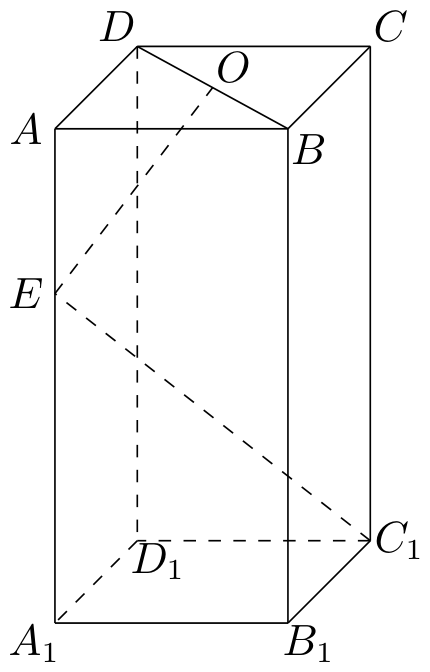
\includegraphics[width=4.2cm]{GaoKao/images/2012/anhui_liberal/q19_fig1.png}
\end{center}

        \item 如图，\(F_{1}\)，\(F_{2}\) 分别是椭圆 \(C: \frac{x^{2}}{a^{2}} + \frac{y^{2}}{b^{2}} = 1 \) （\(a > b > 0\)）的左，右焦点，\(A\) 是椭圆 \(C\) 的顶点；\(B\) 是直线 \(AF_{2}\) 与椭圆 \(C\) 的另一个交点，\(\angle F_{1}AF_{2} = 60^{\circ}\).

\begin{enumerate}
\item 求椭圆 \(C\) 的离心率；
\item 已知 \(\triangle AF_{1}B\) 面积为 \(40\sqrt{3}\)，求 \(a\)，\(b\) 的值.
\end{enumerate}

\begin{center}
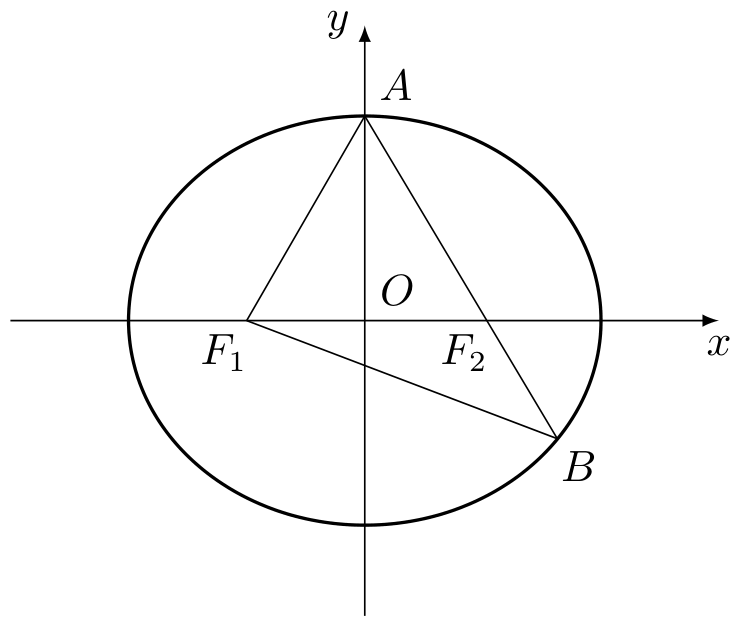
\includegraphics[width=8.9cm]{GaoKao/images/2012/anhui_liberal/q20_fig1.png}
\end{center}

        \item 设 \(f(x) = \frac{x}{2} + \sin x\) 的所有正的极小值点从小到大排成的数列为 \(\{x_n\}\).

\begin{enumerate}
\item 求数列 \(\{x_n\}\) 的通项公式；
\item 设 \(\{x_n\}\) 的前 \(n\) 项和为 \(S_n\)，求 \(\sin S_n\).
\end{enumerate}

    \end{enumerate}

\end{description}


\subsection{2012年北京卷（理）}\label{gk:2012年北京卷（理）}

\begin{description}

    \item[一、选择题]

    \begin{enumerate}[leftmargin=5pt]

        \item 已知集合 \(A = \{x \in \mathbb{R} \mid 3x + 2 > 0\}\)，\(B = \{x \in \mathbb{R} \mid (x + 1)(x - 3) > 0\}\)，则 \(A \cap B =\)（\quad）

        {\centering\begin{tabular*}{\linewidth}{@{}@{\extracolsep{\fill}}llll@{}}
          \text{A. }\((-\infty, -1)\)  &  \text{B. }\(\left(-1, -\frac{2}{3}\right)\)  &  \text{C. }\(\left(-\frac{2}{3}, 3\right)\)  &  \text{D. }\((3, +\infty)\)
        \end{tabular*}\par}

        \item 设不等式组 \(\begin{cases}
0 \leqslant x \leqslant 2,\\
0 \leqslant y \leqslant 2
\end{cases}\) 表示的平面区域为 \(D\). 在区域 \(D\) 内随机取一个点，则此点到坐标原点的距离大于 2 的概率是（\quad）

        {\centering\begin{tabular*}{\linewidth}{@{}@{\extracolsep{\fill}}llll@{}}
          \text{A. }\(\frac{\pi}{4}\)  &  \text{B. }\(\frac{\pi - 2}{2}\)  &  \text{C. }\(\frac{\pi}{6}\)  &  \text{D. }\(\frac{4 - \pi}{4}\)
        \end{tabular*}\par}

        \item 设 \(a\)，\(b \in \mathbb{R}\). “\(a=0\)”是“复数 \(a+b\i\) 是纯虚数”的（\quad）

        {\centering\begin{tabular*}{\linewidth}{@{}@{\extracolsep{\fill}}llll@{}}
          \text{A. }充分而不必要条件  &  \text{B. }必要而不充分条件  &  \text{C. }充分必要条件  &  \text{D. }既不充分也不必要条件
        \end{tabular*}\par}

        \item 执行如图所示的程序框图，输出的 \(S\) 值为（\quad）

\begin{center}
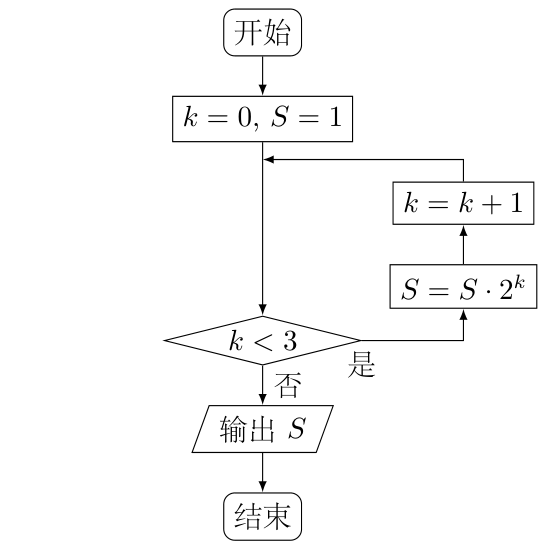
\includegraphics[width=0.70\linewidth]{GaoKao/images/2012/beijing_science/q4_fig1.png}
\end{center}

        {\centering\begin{tabular*}{\linewidth}{@{}@{\extracolsep{\fill}}llll@{}}
          \text{A. }2  &  \text{B. }4  &  \text{C. }8  &  \text{D. }16
        \end{tabular*}\par}

        \item 如图，\(\angle ACB = 90^{\circ}\)，\(CD \perp AB\) 于点 \(D\)，以 \(BD\) 为直径的圆与 \(BC\) 交于点 \(E\)，则（\quad）

\begin{center}
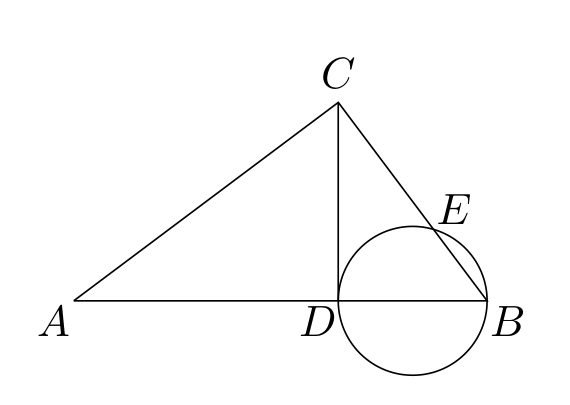
\includegraphics[width=5.6cm]{GaoKao/images/2012/beijing_science/q5_fig1.png}
\end{center}

        {\centering\begin{tabular*}{\linewidth}{@{}@{\extracolsep{\fill}}llll@{}}
          \text{A. }\(CE \cdot CB = AD \cdot DB\)  &  \text{B. }\(CE\cdot CB = AD\cdot AB\)  &  \text{C. }\(AD\cdot AB = CD^{2}\)  &  \text{D. }\(CE\cdot EB = CD^{2}\)
        \end{tabular*}\par}

        \item 从 \(0\)，\(2\) 中选一个数字，从 \(1\)，\(3\)，\(5\) 中选两个数字，组成无重复数字的三位数，其中奇数的个数为（\quad）

        {\centering\begin{tabular*}{\linewidth}{@{}@{\extracolsep{\fill}}llll@{}}
          \text{A. }24  &  \text{B. }18  &  \text{C. }12  &  \text{D. }6
        \end{tabular*}\par}

        \item 某三棱锥的三视图如图所示，该三棱锥的表面积是（\quad）

\begin{center}
\includegraphics[width=6.4cm]{GaoKao/images/2012/beijing_science/q7_fig1.png}
\end{center}

        {\centering\begin{tabular*}{\linewidth}{@{}@{\extracolsep{\fill}}llll@{}}
          \text{A. }\(28 + 6\sqrt{5}\)  &  \text{B. }\(30 + 6\sqrt{5}\)  &  \text{C. }\(56 + 12\sqrt{5}\)  &  \text{D. }\(60 + 12\sqrt{5}\)
        \end{tabular*}\par}

        \item 某棵果树前 \(n\) 年的总产量 \(S_n\) 与 \(n\) 之间的关系如图所示. 从目前记录的结果看，前 \(m\) 年的年平均产量最高，\(m\) 的值为（\quad）

\begin{center}
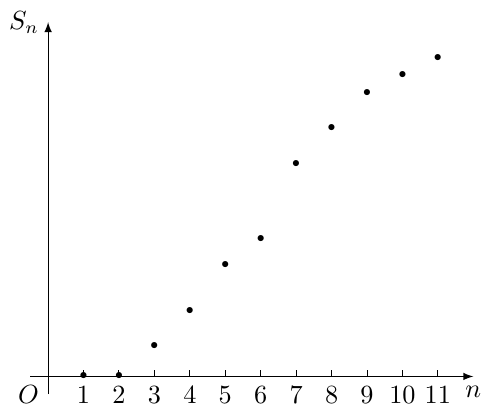
\includegraphics[width=8.9cm]{GaoKao/images/2012/beijing_science/q8_fig1.png}
\end{center}

        {\centering\begin{tabular*}{\linewidth}{@{}@{\extracolsep{\fill}}llll@{}}
          \text{A. }5  &  \text{B. }7  &  \text{C. }9  &  \text{D. }11
        \end{tabular*}\par}

    \end{enumerate}

\end{description}

\begin{description}

    \item[二、填空题]

    \begin{enumerate}[leftmargin=5pt]

      \addtocounter{enumi}{+8}

        \item 直线 \(\begin{cases}
x=2+t,\\
y=-1-t,
\end{cases}\)（\(t\) 为参数）与曲线 \(\begin{cases}
x=3\cos\alpha,\\
y=3\sin\alpha,
\end{cases}\)（\(\alpha\) 为参数）的交点个数为\rule[-0.3ex]{3em}{0.4pt}.

        \item 已知 \(\{a_n\}\) 为等差数列，\(S_n\) 为其前 \(n\) 项和，若 \(a_1=\frac{1}{2}\)，\(S_2=a_3\)，则 \(a_2=\)\rule[-0.3ex]{3em}{0.4pt}；\(S_n=\)\rule[-0.3ex]{3em}{0.4pt}.

        \item 在 \(\triangle ABC\) 中，若 \(a=2\)，\(b+c=7\)，\(\cos B=-\frac{1}{4}\)，则 \(b=\)\rule[-0.3ex]{3em}{0.4pt}.

        \item 在直角坐标系 \(xOy\) 中，直线 \(l\) 过抛物线 \(y^2 = 4x\) 的焦点 \(F\)，且与该抛物线相交于 \(A\)，\(B\) 两点，其中点 \(A\) 在 \(x\) 轴上方. 若直线 \(l\) 的倾斜角为 \(60^\circ\)，则 \(\triangle OAF\) 的面积为\rule[-0.3ex]{3em}{0.4pt}.

        \item 已知正方形 \(ABCD\) 的边长为 1，点 \(E\) 是 \(AB\) 边上的动点，则 \(\overrightarrow{DE} \cdot \overrightarrow{CB}\) 的值为\rule[-0.3ex]{3em}{0.4pt}；\(\overrightarrow{DE} \cdot \overrightarrow{DC}\) 的最大值为\rule[-0.3ex]{3em}{0.4pt}.

        \item 已知 \(f(x)=m(x-2m)(x+m+3)\)，\(g(x)=2^x-2\). 若同时满足条件：

\begin{enumerate}
\item \(\forall x\in\mathbb{R}\)，\(f(x)<0\) 或 \(g(x)<0\)；
\item \(\exists x\in(-\infty,-4)\)，\(f(x)g(x)<0\)，
\end{enumerate}

则 \(m\) 的取值范围是\rule[-0.3ex]{3em}{0.4pt}.

    \end{enumerate}

\end{description}

\begin{description}

    \item[三、解答题]

    \begin{enumerate}[leftmargin=5pt]

      \addtocounter{enumi}{+14}

        \item 已知函数 \(f(x)=\frac{(\sin x-\cos x)\sin 2x}{\sin x}\).

\begin{enumerate}
\item 求 \(f(x)\) 的定义域及最小正周期；
\item 求 \(f(x)\) 的单调递增区间.
\end{enumerate}

        \item 如图 1，在 \(\mathrm{Rt}\triangle ABC\) 中，\(\angle C=90^\circ\)，\(BC=3\)，\(AC=6\). \(D\)，\(E\) 分别是 \(AC\)，\(AB\) 上的点，且 \(DE\parallel BC\)，\(DE=2\)，将 \(\triangle ADE\) 沿 \(DE\) 折起到 \(\triangle A_1DE\) 的位置，使 \(A_1C \perp CD\)，如图 2.

\begin{enumerate}
\item 求证：\(A_1C \perp\) 平面 \(BCDE\)；
\item 若 \(M\) 是 \(A_1D\) 的中点，求 \(CM\) 与平面 \(A_1BE\) 所成角的大小；
\item 线段 \(BC\) 上是否存在点 \(P\)，使平面 \(A_1DP\) 与平面 \(A_1BE\) 垂直？说明理由.
\end{enumerate}

\begin{center}
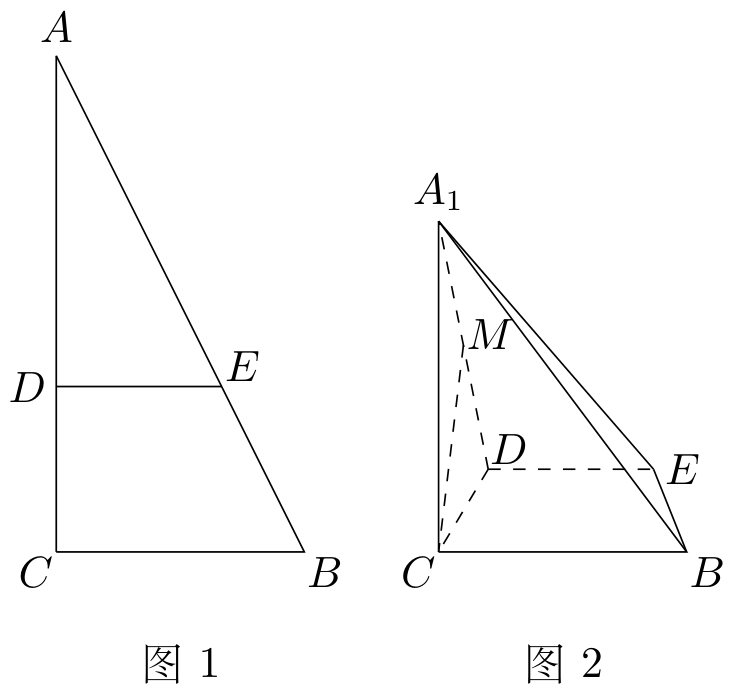
\includegraphics[width=7.3cm]{GaoKao/images/2012/beijing_science/q16_fig1.png}
\end{center}

        \item 近年来，某市为促进生活垃圾的分类处理，将生活垃圾分为厨余垃圾，可回收物和其他垃圾三类，并分别设置了相应的垃圾箱. 为调查居民生活垃圾分类投放情况，现随机抽取了该市三类垃圾箱中总计 \(1000\text{ 吨}\) 生活垃圾，数据统计如下（单位：\(\text{吨}\)）：

\begin{center}
\renewcommand{\arraystretch}{1.2}
\begin{tabular}{|c|c|c|c|}
\hline
& “厨余垃圾”箱 & “可回收物”箱 & “其他垃圾”箱 \\
\hline
厨余垃圾 & 400 & 100 & 100 \\
\hline
可回收物 & 30 & 240 & 30 \\
\hline
其他垃圾 & 20 & 20 & 60 \\
\hline
\end{tabular}
\end{center}

\begin{enumerate}
\item 试估计厨余垃圾投放正确的概率；
\item 试估计生活垃圾投放错误的概率；
\item 假设厨余垃圾在“厨余垃圾”箱，“可回收物”箱，“其他垃圾”箱的投放量分别为 \(a\)，\(b\)，\(c\)，其中 \(a>0\)，\(a+b+c=600\). 当数据 \(a\)，\(b\)，\(c\) 的方差 \(s^2\) 最大时，写出 \(a\)，\(b\)，\(c\) 的值（结论不要求证明），并求此时 \(s^2\) 的值.
\end{enumerate}

（注：\(s^2=\frac{1}{n}\left[(x_1-\overline{x})^2+(x_2-\overline{x})^2+\cdots+(x_n-\overline{x})^2\right]\)，其中 \(\overline{x}\) 为数据 \(x_1\)，\(x_2\)，\(\cdots\)，\(x_n\) 的平均数）

        \item 已知函数 \(f(x)=ax^2+1\)（\(a>0\)），\(g(x)=x^3+bx\).

\begin{enumerate}
\item 若曲线 \(y=f(x)\) 与曲线 \(y=g(x)\) 在它们的交点 \((1,c)\) 处具有公共切线，求 \(a\)，\(b\) 的值；
\item 当 \(a^2=4b\) 时，求函数 \(f(x)+g(x)\) 的单调区间，并求其在区间 \((-\infty,-1]\) 上的最大值.
\end{enumerate}

        \item 已知曲线 \(C:(5-m)x^2+(m-2)y^2=8\)（\(m\in\mathbb{R}\)）.

\begin{enumerate}
\item 若曲线 \(C\) 是焦点在 \(x\) 轴上的椭圆，求 \(m\) 的取值范围；
\item 设 \(m=4\)，曲线 \(C\) 与 \(y\) 轴的交点为 \(A\)，\(B\)（点 \(A\) 位于点 \(B\) 的上方），直线 \(y=kx+4\) 与曲线 \(C\) 交于不同的两点 \(M\)，\(N\)，直线 \(y=1\) 与直线 \(BM\) 交于点 \(G\). 求证：\(A\)，\(G\)，\(N\) 三点共线.
\end{enumerate}

        \item 设 \(A\) 是由 \(m\times n\) 个实数组成的 \(m\) 行 \(n\) 列的数表，满足：每个数的绝对值不大于 1，且所有数的和为零. 记 \(S(m,n)\) 为所有这样的数表构成的集合. 对于 \(A\in S(m,n)\)，记 \(r_i(A)\) 为 \(A\) 的第 \(i\) 行各数之和（\(1\le i\le m\)），\(c_j(A)\) 为 \(A\) 的第 \(j\) 列各数之和（\(1\le j\le n\)）；记 \(k(A)\) 为 \(|r_1(A)|\)，\(|r_2(A)|\)，\(\cdots\)，\(|r_m(A)|\)，\(|c_1(A)|\)，\(|c_2(A)|\)，\(\cdots\)，\(|c_n(A)|\) 中的最小值.

\begin{enumerate}
\item 对如下数表 \(A\)，求 \(k(A)\) 的值：

\begin{center}
\renewcommand{\arraystretch}{1.2}
\begin{tabular}{|c|c|c|}
\hline
1 & 1 & \(-0.8\) \\
\hline
\(0.1\) & \(-0.3\) & \(-1\) \\
\hline
\end{tabular}
\end{center}

\item 设数表 \(A\in S(2,3)\) 形如

\begin{center}
\renewcommand{\arraystretch}{1.2}
\begin{tabular}{|c|c|c|}
\hline
1 & 1 & \(c\) \\
\hline
\(a\) & \(b\) & \(-1\) \\
\hline
\end{tabular}
\end{center}

求 \(k(A)\) 的最大值；
\item 给定正整数 \(t\)，对于所有的 \(A\in S(2,2t+1)\)，求 \(k(A)\) 的最大值.
\end{enumerate}

    \end{enumerate}

\end{description}


\subsection{2012年北京卷（文）}\label{gk:2012年北京卷（文）}

\begin{description}

    \item[一、选择题]

    \begin{enumerate}[leftmargin=5pt]

        \item 已知集合 \(A = \{x \in \mathbb{R} \mid 3x + 2 > 0\}\)，\(B = \{x \in \mathbb{R} \mid (x + 1)(x - 3) > 0\}\)，则 \(A \cap B =\)（\quad）

        {\centering\begin{tabular*}{\linewidth}{@{}@{\extracolsep{\fill}}llll@{}}
          \text{A. }\((-\infty, -1)\)  &  \text{B. }\(\left(-1, -\frac{2}{3}\right)\)  &  \text{C. }\(\left(-\frac{2}{3}, 3\right)\)  &  \text{D. }\((3, +\infty)\)
        \end{tabular*}\par}

        \item 在复平面内，复数 \(\frac{10\i}{3 + \i}\) 对应的点的坐标为（\quad）

        {\centering\begin{tabular*}{\linewidth}{@{}@{\extracolsep{\fill}}llll@{}}
          \text{A. }\((1,3)\)  &  \text{B. }\((3,1)\)  &  \text{C. }\((-1,3)\)  &  \text{D. }\((3,-1)\)
        \end{tabular*}\par}

        \item 设不等式组
\[
\begin{cases}

0 \leqslant x \leqslant 2,\\
0 \leqslant y \leqslant 2

\end{cases}
\]表示的平面区域为 \(D\). 在区域 \(D\) 内随机取一个点，则此点到坐标原点的距离大于 \(2\) 的概率是（\quad）

        {\centering\begin{tabular*}{\linewidth}{@{}@{\extracolsep{\fill}}llll@{}}
          \text{A. }\(\frac{\pi}{4}\)  &  \text{B. }\(\frac{\pi - 2}{2}\)  &  \text{C. }\(\frac{\pi}{6}\)  &  \text{D. }\(\frac{4 - \pi}{4}\)
        \end{tabular*}\par}

        \item 执行如图所示的程序框图，输出的 \(S\) 值为（\quad）

\begin{center}
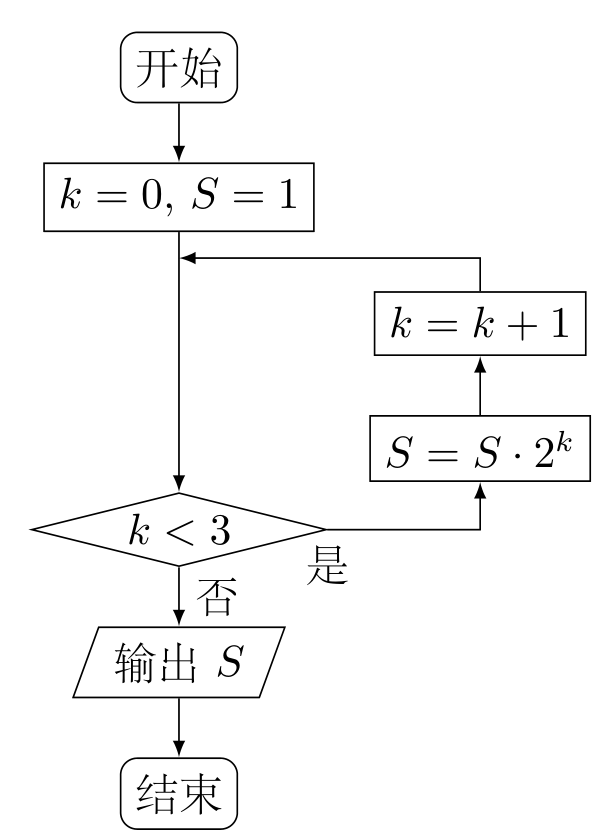
\includegraphics[width=5.8cm]{GaoKao/images/2012/beijing_liberal/q4_fig1.png}
\end{center}

        {\centering\begin{tabular*}{\linewidth}{@{}@{\extracolsep{\fill}}llll@{}}
          \text{A. }\(2\)  &  \text{B. }\(4\)  &  \text{C. }\(8\)  &  \text{D. }\(16\)
        \end{tabular*}\par}

        \item 函数 \(f(x) = x^{\frac{1}{2}} - \left(\frac{1}{2}\right)^x\) 的零点个数为（\quad）

        {\centering\begin{tabular*}{\linewidth}{@{}@{\extracolsep{\fill}}llll@{}}
          \text{A. }\(0\)  &  \text{B. }\(1\)  &  \text{C. }\(2\)  &  \text{D. }\(3\)
        \end{tabular*}\par}

        \item 已知 \(\{a_n\}\) 为等比数列，下面结论中正确的是（\quad）

        {\centering\begin{tabular*}{\linewidth}{@{}@{\extracolsep{\fill}}llll@{}}
          \text{A. }\(a_{1} + a_{3} \geqslant 2a_{2}\)  &  \text{B. }\(a_{1}^{2} + a_{3}^{2} \geqslant 2a_{2}^{2}\)  &  \text{C. }\(\text{若\ } a_{1} = a_{3}\)，\(\text{ 则 } a_{1} = a_{2}\)  &  \text{D. }\(\text{若\ } a_{3} > a_{1}\)，\(\text{ 则 } a_{4} > a_{2}\)
        \end{tabular*}\par}

        \item 某三棱锥的三视图如图所示，该三棱锥的表面积是（\quad）

\begin{center}
\includegraphics[width=6.4cm]{GaoKao/images/2012/beijing_liberal/q7_fig1.png}
\end{center}

        {\centering\begin{tabular*}{\linewidth}{@{}@{\extracolsep{\fill}}llll@{}}
          \text{A. }\(28 + 6\sqrt{5}\)  &  \text{B. }\(30 + 6\sqrt{5}\)  &  \text{C. }\(56 + 12\sqrt{5}\)  &  \text{D. }\(60 + 12\sqrt{5}\)
        \end{tabular*}\par}

        \item 某果树前 \(n\) 年的总产量 \(S_n\) 与 \(n\) 之间的关系如图所示. 从目前记录的结果看，前 \(m\) 年的年平均产量最高，\(m\) 的值为（\quad）

\begin{center}
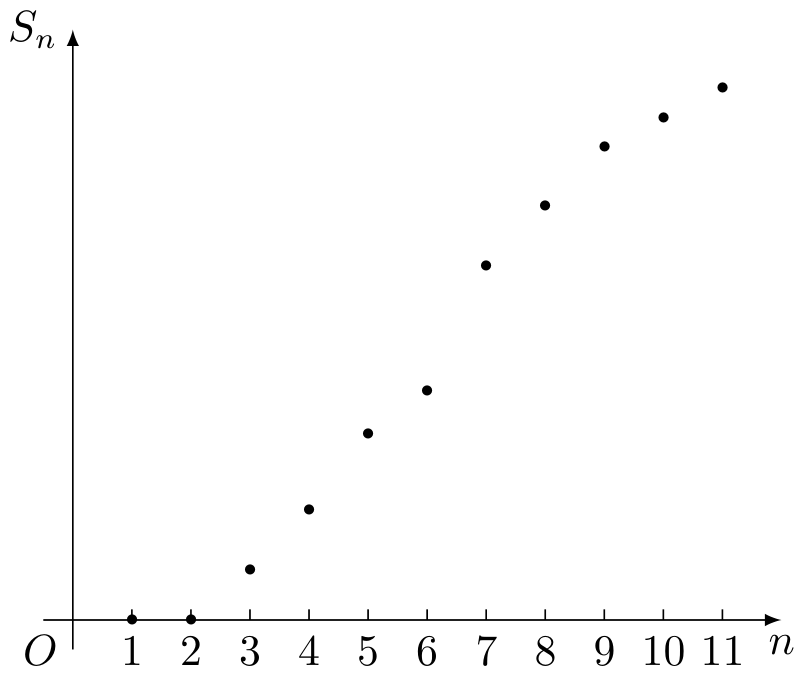
\includegraphics[width=9.7cm]{GaoKao/images/2012/beijing_liberal/q8_fig1.png}
\end{center}

        {\centering\begin{tabular*}{\linewidth}{@{}@{\extracolsep{\fill}}llll@{}}
          \text{A. }5  &  \text{B. }7  &  \text{C. }9  &  \text{D. }11
        \end{tabular*}\par}

    \end{enumerate}

\end{description}

\begin{description}

    \item[二、填空题]

    \begin{enumerate}[leftmargin=5pt]

      \addtocounter{enumi}{+8}

        \item 直线 \(y = x\) 被圆 \(x^2 + (y - 2)^2 = 4\) 截得的弦长为\rule[-0.3ex]{3em}{0.4pt}.

        \item 已知 \(\{a_n\}\) 为等差数列，\(S_n\) 为其前 \(n\) 项和，若 \(a_1 = \frac{1}{2}\)，\(S_2 = a_3\)，则 \(a_2=\)\rule[-0.3ex]{3em}{0.4pt}；\(S_n=\)\rule[-0.3ex]{3em}{0.4pt}.

        \item 在 \(\triangle ABC\) 中，若 \(a = 3\)，\(b = \sqrt{3}\)，\(\angle A = \frac{\pi}{3}\)，则 \(\angle C\) 的大小为\rule[-0.3ex]{3em}{0.4pt}.

        \item 已知函数 \(f(x) = \lg x\). 若 \(f(ab) = 1\)，则 \(f(a^2) + f(b^2)=\)\rule[-0.3ex]{3em}{0.4pt}.

        \item 已知正方形 \(ABCD\) 的边长为 \(1\)，点 \(E\) 是 \(AB\) 边上的动点，则 \(\overrightarrow{DE} \cdot \overrightarrow{CB}\) 的值为\rule[-0.3ex]{3em}{0.4pt}；\(\overrightarrow{DE} \cdot \overrightarrow{DC}\) 的最大值为\rule[-0.3ex]{3em}{0.4pt}.

        \item 已知 \(f(x) = m(x - 2m)(x + m + 3)\)，\(g(x) = 2^{x} - 2\). 若 \(\forall x \in \mathbb{R}\)，\(f(x) < 0\) 或 \(g(x) < 0\)，则 \(m\) 的取值范围是\rule[-0.3ex]{3em}{0.4pt}.

    \end{enumerate}

\end{description}

\begin{description}

    \item[三、解答题]

    \begin{enumerate}[leftmargin=5pt]

      \addtocounter{enumi}{+14}

        \item 已知函数 \( f(x) = \dfrac{(\sin x - \cos x)\sin 2x}{\sin x} \).
\begin{enumerate}
\item 求 \( f(x) \) 的定义域及最小正周期；
\item 求 \( f(x) \) 的单调递减区间.
\end{enumerate}

        \item 如图 1，在 \(\mathrm{Rt}\triangle ABC\) 中，\(\angle C = 90^\circ\)，\(D\)，\(E\) 分别是 \(AC\)，\(AB\) 的中点，点 \(F\) 为线段 \(CD\) 上的一点，将 \(\triangle ADE\) 沿 \(DE\) 折起到 \(\triangle A_1DE\) 的位置，使 \(A_1F \perp CD\)，如图 2.

\begin{enumerate}
\item 求证：\(DE\parallel\text{平面 }A_1CB\)；
\item 求证：\(A_1F\perp BE\)；
\item 线段 \(A_1B\) 上是否存在点 \(Q\)，使 \(A_1C\perp\text{平面 }DEQ\)？说明理由.
\end{enumerate}

\begin{center}
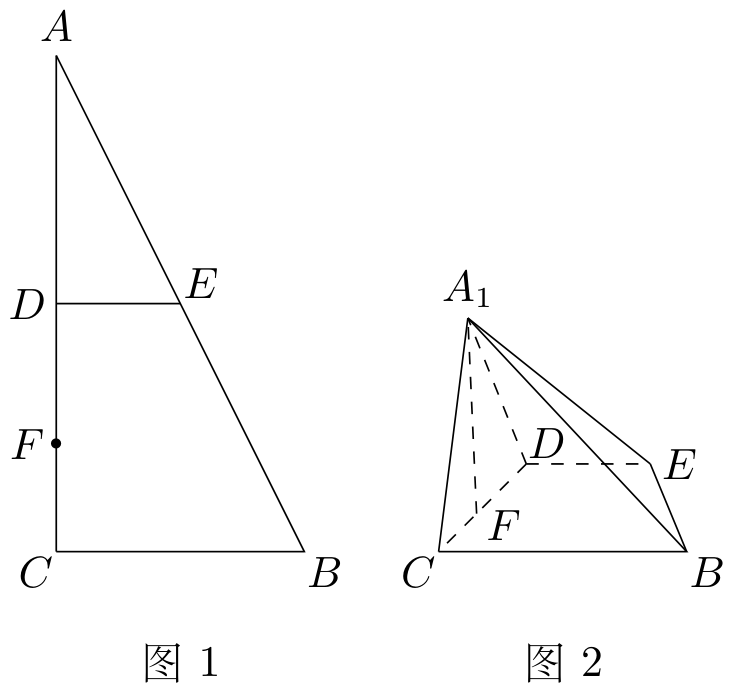
\includegraphics[width=7.3cm]{GaoKao/images/2012/beijing_liberal/q16_fig1.png}
\end{center}

        \item 近年来，某市为促进生活垃圾的分类处理，将生活垃圾分为厨余垃圾，可回收物和其他垃圾三类，并分别设置了相应的垃圾箱. 为调查居民生活垃圾分类投放情况，现随机抽取了该市三类垃圾箱中总计 \(1000\text{ 吨}\) 生活垃圾，数据统计如下（单位：吨）：

\begin{center}
\begin{tabular}{c|ccc}
 & “厨余垃圾”箱 & “可回收物”箱 & “其他垃圾”箱 \\
\hline
厨余垃圾 & 400 & 100 & 100 \\
可回收物 & 30 & 240 & 30 \\
其他垃圾 & 20 & 20 & 60
\end{tabular}
\end{center}

\begin{enumerate}
\item 试估计厨余垃圾投放正确的概率；
\item 试估计生活垃圾投放错误的概率；
\item 假设厨余垃圾在“厨余垃圾”箱，“可回收物”箱，“其他垃圾”箱的投放量分别为 \(a\)，\(b\)，\(c\)，其中 \(a > 0\)，\(a + b + c = 600\). 当数据 \(a\)，\(b\)，\(c\) 的方差 \(s^2\) 最大时，写出 \(a\)，\(b\)，\(c\) 的值（结论不要求证明），并求此时 \(s^2\) 的值.
\end{enumerate}

（注：\(s^2 = \frac{1}{n}\left[(x_1 - \overline{x})^2 + (x_2 - \overline{x})^2 + \cdots + (x_n - \overline{x})^2\right]\)，其中 \(\overline{x}\) 为 \(x_1\)，\(x_2\)，\(\cdots\)，\(x_n\) 的平均数）

        \item 已知函数 \(f(x) = ax^2 + 1\) （\(a > 0\)），\(g(x) = x^3 + bx\).
\begin{enumerate}
\item 若曲线 \(y = f(x)\) 与曲线 \(y = g(x)\) 在它们的交点 \((1, c)\) 处具有公共切线，求 \(a\)，\(b\) 的值；
\item 当 \(a = 3\)，\(b = -9\) 时，若函数 \(f(x) + g(x)\) 在区间 \([k, 2]\) 上的最大值为 28，求 \(k\) 的取值范围.
\end{enumerate}

        \item 已知椭圆 \(C: \frac{x^2}{a^2} + \frac{y^2}{b^2} = 1\) （\(a > b > 0\)）的一个顶点为 \(A(2, 0)\)，离心率为 \(\frac{\sqrt{2}}{2}\)，直线 \(y = k(x - 1)\) 与椭圆 \(C\) 交于不同的两点 \(M\)，\(N\).

\begin{enumerate}
\item 求椭圆 \(C\) 的方程；
\item 当 \(\triangle AMN\) 的面积为 \(\frac{\sqrt{10}}{3}\) 时，求 \(k\) 的值.
\end{enumerate}

        \item 设 \(A\) 是如下形式的 2 行 3 列的数表，

\[
\begin{array}{ccc}

a & b & c \\
d & e & f

\end{array}
\]满足性质 \(P\)：\(a\)，\(b\)，\(c\)，\(d\)，\(e\)，\(f \in [-1, 1]\)，且 \(a + b + c + d + e + f = 0\).
记 \(r_i(A)\) 为 \(A\) 的第 \(i\) 行各数之和 （\(i = 1, 2\)），\(c_j(A)\) 为 \(A\) 的第 \(j\) 列各数之和 （\(j = 1, 2, 3\)）；记 \(k(A)\) 为 \(|r_1(A)|\)，\(|r_2(A)|\)，\(|c_1(A)|\)，\(|c_2(A)|\)，\(|c_3(A)|\) 中的最小值.

\begin{enumerate}
\item 对如下数表 \(A\)，求 \(k(A)\) 的值；

\[
\begin{array}{ccc}

1 & 1 & -0.8 \\
0.1 & -0.3 & -1

\end{array}
\]\item 设数表 \(A\) 形如

\[
\begin{array}{ccc}

1 & 1 & -1 - 2d \\
d & d & -1

\end{array}
\]其中 \(-1 \leqslant d \leqslant 0\). 求 \(k(A)\) 的最大值；
\item 对所有满足性质 \(P\) 的 2 行 3 列的数表 \(A\)，求 \(k(A)\) 的最大值.
\end{enumerate}

    \end{enumerate}

\end{description}


\subsection{2012年重庆卷（理）}\label{gk:2012年重庆卷（理）}

\begin{description}

    \item[一、选择题]

    \begin{enumerate}[leftmargin=5pt]

        \item 在等差数列 \(\{a_{n}\}\) 中，\(a_{2} = 1\)，\(a_{4} = 5\)，则 \(\{a_{n}\}\) 的前 5 项和 \(S_{5} =\)（\quad）

        {\centering\begin{tabular*}{\linewidth}{@{}@{\extracolsep{\fill}}llll@{}}
          \text{A. }\(7\)  &  \text{B. }\(15\)  &  \text{C. }\(20\)  &  \text{D. }\(25\)
        \end{tabular*}\par}

        \item 不等式 \(\frac{x - 1}{2x + 1} \leqslant 0\) 的解集为（\quad）

        {\centering\begin{tabular*}{\linewidth}{@{}@{\extracolsep{\fill}}llll@{}}
          \text{A. }\( \left(-\frac{1}{2},1\right] \)  &  \text{B. }\( \left[-\frac{1}{2},1\right] \)  &  \text{C. }\(\left(-\infty, -\frac{1}{2}\right) \cup [1, +\infty)\)  &  \text{D. }\(\left(-\infty, -\frac{1}{2}\right] \cup [1, +\infty)\)
        \end{tabular*}\par}

        \item 对任意的实数 \(k\)，直线 \(y = kx + 1\) 与圆 \(x^{2} + y^{2} = 2\) 的位置关系一定是（\quad）

        {\centering\begin{tabular*}{\linewidth}{@{}@{\extracolsep{\fill}}llll@{}}
          \text{A. }相离  &  \text{B. }相切  &  \text{C. }相交但直线不过圆心  &  \text{D. }相交且直线过圆心
        \end{tabular*}\par}

        \item \(\left(\sqrt{x} +\frac{1}{2\sqrt{x}}\right)^8\) 的展开式中常数项为（\quad）

        {\centering\begin{tabular*}{\linewidth}{@{}@{\extracolsep{\fill}}llll@{}}
          \text{A. }\(\frac{35}{16}\)  &  \text{B. }\(\frac{35}{8}\)  &  \text{C. }\(\frac{35}{4}\)  &  \text{D. }\(105\)
        \end{tabular*}\par}

        \item 设 \(\tan \alpha\)，\(\tan \beta\) 是方程 \(x^{2} - 3x + 2 = 0\) 的两根，则 \(\tan (\alpha + \beta)\) 的值为（\quad）

        {\centering\begin{tabular*}{\linewidth}{@{}@{\extracolsep{\fill}}llll@{}}
          \text{A. }\(-3\)  &  \text{B. }\(-1\)  &  \text{C. }\(1\)  &  \text{D. }\(3\)
        \end{tabular*}\par}

        \item 设 \(x\)，\(y \in \mathbb{R}\)，向量 \(\bm{a} = (x, 1)\)，\(\bm{b} = (1, y)\)，\(\bm{c} = (2, -4)\)，且 \(\bm{a} \perp \bm{c}\)，\(\bm{b} \parallel \bm{c}\)，则 \(|\bm{a} + \bm{b}| =\)（\quad）

        {\centering\begin{tabular*}{\linewidth}{@{}@{\extracolsep{\fill}}llll@{}}
          \text{A. }\(\sqrt{5}\)  &  \text{B. }\(\sqrt{10}\)  &  \text{C. }\(2\sqrt{5}\)  &  \text{D. }\(10\)
        \end{tabular*}\par}

        \item 已知 \(f(x)\) 是定义在 \(\mathbb{R}\) 上的偶函数，且以 2 为周期，则 \(f(x)\) 为 \([0,1]\) 上的增函数是“\(f(x)\) 为 \([3,4]\) 上的减函数”的（\quad）

        {\centering\begin{tabular*}{\linewidth}{@{}@{\extracolsep{\fill}}llll@{}}
          \text{A. }既不充分也不必要的条件  &  \text{B. }充分而不必要的条件  &  \text{C. }必要而不充分的条件  &  \text{D. }充要条件
        \end{tabular*}\par}

        \item 设函数 \( f(x) \) 在 \( \mathbb{R} \) 上可导，其导函数为 \( f'(x) \)，且函数 \( y = (1 - x)f'(x) \) 的图象如图所示，则下列结论中一定成立的是（\quad）

\begin{center}
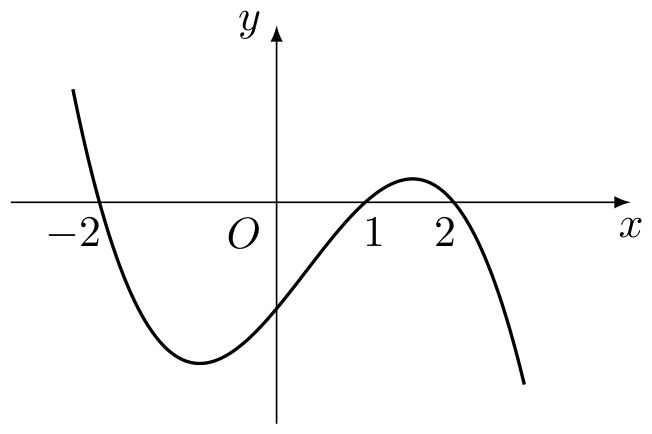
\includegraphics[width=8.1cm]{GaoKao/images/2012/chongqing_science/q8_fig1.png}
\end{center}

        {\centering\begin{tabular*}{\linewidth}{@{}@{\extracolsep{\fill}}llll@{}}
          \text{A. }函数 \( f(x) \) 有极大值 \( f(2) \) 和极小值 \( f(1) \)  &  \text{B. }函数 \( f(x) \) 有极大值 \( f(-2) \) 和极小值 \( f(1) \)  &  \text{C. }函数 \( f(x) \) 有极大值 \( f(2) \) 和极小值 \( f(-2) \)  &  \text{D. }函数 \( f(x) \) 有极大值 \( f(-2) \) 和极小值 \( f(2) \)
        \end{tabular*}\par}

        \item 设四面体的六条棱的长分别为 \(1\)，\(1\)，\(1\)，\(1\)，\(\sqrt{2}\) 和 \(a\)，且长为 \(a\) 的棱与长为 \(\sqrt{2}\) 的棱异面，则 \(a\) 的取值范围是（\quad）

        {\centering\begin{tabular*}{\linewidth}{@{}@{\extracolsep{\fill}}llll@{}}
          \text{A. }\((0, \sqrt{2})\)  &  \text{B. }\((0, \sqrt{3})\)  &  \text{C. }\((1, \sqrt{2})\)  &  \text{D. }\((1, \sqrt{3})\)
        \end{tabular*}\par}

        \item 设平面点集 \(A = \left\{(x, y) \mid (y - x)\left(y - \frac{1}{x}\right) \geqslant 0\right\}\)，\(B = \{(x, y) \mid (x - 1)^2 + (y - 1)^2 \leqslant 1\}\)，则 \(A \cap B\) 所表示的平面图形的面积为（\quad）

        {\centering\begin{tabular*}{\linewidth}{@{}@{\extracolsep{\fill}}llll@{}}
          \text{A. }\(\frac{3}{4}\pi\)  &  \text{B. }\(\frac{3}{5}\pi\)  &  \text{C. }\(\frac{4}{7}\pi\)  &  \text{D. }\(\frac{\pi}{2}\)
        \end{tabular*}\par}

    \end{enumerate}

\end{description}

\begin{description}

    \item[二、填空题]

    \begin{enumerate}[leftmargin=5pt]

      \addtocounter{enumi}{+10}

        \item 若 \( (1 + i)(2 + i) = a + bi \)，其中 \(a\)，\(b \in \mathbb{R}\)，\(i\) 为虚数单位，则 \( a + b = \)\rule[-0.3ex]{3em}{0.4pt}.

        \item \(\displaystyle\lim_{n\to\infty}\frac{1}{\sqrt{n^2 + 5n} - n}=\)\rule[-0.3ex]{3em}{0.4pt}.

        \item 设 \(\triangle ABC\) 的内角 \(A\)，\(B\)，\(C\) 所对的边分别为 \(a\)，\(b\)，\(c\)，且 \(\cos A = \frac{3}{5}\)，\(\cos B = \frac{5}{13}\)，\(b = 3\)，则 \(c =\rule[-0.3ex]{3em}{0.4pt}\).

        \item 过抛物线 \(y^{2}=2x\) 的焦点 \(F\) 作直线 \(l\) 交抛物线于 \(A\)，\(B\) 两点，若 \(|AB|=\frac{25}{12}\)，\(|AF|<|BF|\)，则 \(|AF|=\)\rule[-0.3ex]{3em}{0.4pt}.

        \item 某艺校在一天的 \(6\) 节课中随机安排语文、数学、外语三门文化课和其他三门艺术课各 \(1\) 节，则在课表上的相邻两节文化课之间最多间隔 \(1\) 节艺术课的概率为\rule[-0.3ex]{3em}{0.4pt}.

    \end{enumerate}

\end{description}

\begin{description}

    \item[三、解答题]

    \begin{enumerate}[leftmargin=5pt]

      \addtocounter{enumi}{+15}

        \item 设 \( f(x)=a\ln x+\frac{1}{2x}+\frac{3}{2}x+1 \)，其中 \( a\in \mathbb{R} \)，曲线 \( y=f(x) \) 在点 \( (1,f(1)) \) 处的切线垂直于 \(y\) 轴.
\begin{enumerate}
\item 求 \(a\) 的值；
\item 求函数 \( f(x) \) 的极值.
\end{enumerate}

        \item 甲，乙两人轮流投篮. 每人每次投一球. 约定甲先投且先投中者获胜，一直到有人获胜或每人都已投球 3 次时投篮结束. 设甲每次投篮投中的概率为 \(\frac{1}{3}\)，乙每次投篮投中的概率为 \(\frac{1}{2}\)，且各次投篮互不影响.
\begin{enumerate}
\item 求甲获胜的概率；
\item 求投篮结束时的甲投篮次数 \( \xi \) 的分布列与期望.
\end{enumerate}

        \item 设 \( f(x)=4\cos\left(\omega x-\frac{\pi}{6}\right)\sin\omega x-\cos(2\omega x+\pi) \)，其中 \( \omega>0 \).
\begin{enumerate}
\item 求函数 \( y = f(x) \) 的值域；
\item 若 \( f(x) \) 在区间 \( \left[-\frac{3\pi}{2}, \frac{\pi}{2}\right] \) 上为增函数，求 \( \omega \) 的最大值.
\end{enumerate}

        \item 如图，在直三棱柱 \(ABC - A_{1}B_{1}C_{1}\) 中，\(AB = 4\)，\(AC = BC = 3\)，\(D\) 为 \(AB\) 的中点.
\begin{enumerate}
\item 求点 C 到平面 \(A_{1}ABB_{1}\) 的距离；
\item 若 \(AB_{1} \perp A_{1}C\)，求二面角 \(A_{1} - CD - C_{1}\) 的平面角的余弦值.
\end{enumerate}

\begin{center}
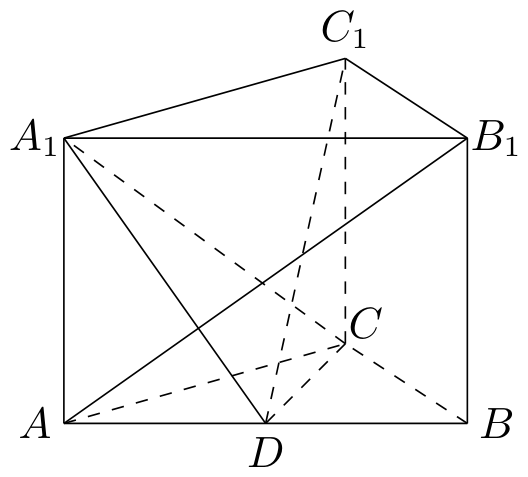
\includegraphics[width=5.6cm]{GaoKao/images/2012/chongqing_science/q19_fig1.png}
\end{center}

        \item 如图，设椭圆的中心为原点 \(O\)，长轴在 \(x\) 轴上，上顶点为 \(A\)，左，右焦点分别为 \(F_{1}\)，\(F_{2}\)，线段 \(OF_{1}\)，\(OF_{2}\) 的中点分别为 \(B_{1}\)，\(B_{2}\)，且 \(\triangle AB_{1}B_{2}\) 是面积为 4 的直角三角形.
\begin{enumerate}
\item 求该椭圆的离心率和标准方程；
\item 过 \(B_{1}\) 作直线 \(l\) 交椭圆于 \(P\)，\(Q\) 两点，使 \(PB_{2} \perp QB_{2}\)，求直线 \(l\) 的方程.
\end{enumerate}

\begin{center}
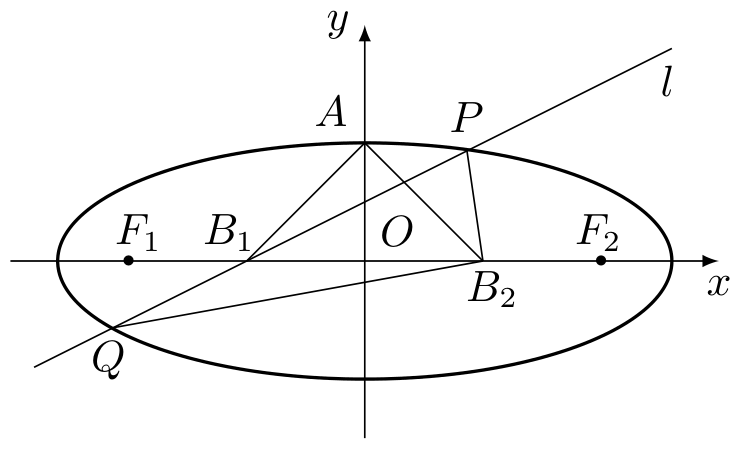
\includegraphics[width=8.6cm]{GaoKao/images/2012/chongqing_science/q20_fig1.png}
\end{center}

        \item 设数列 \(\{a_{n}\}\) 的前 \(n\) 项和 \(S_{n}\) 满足 \(S_{n + 1} = a_2S_n + a_1\)，其中 \(a_2\neq 0\).
\begin{enumerate}
\item 求证： \(\{a_{n}\}\) 是首项为 1 的等比数列；
\item 若 \(a_{2} > -1\)，求证：\(S_{n} \leqslant \frac{n}{2}(a_{1} + a_{n})\)，并给出等号成立的充要条件.
\end{enumerate}

    \end{enumerate}

\end{description}


\subsection{2012年重庆卷（文）}\label{gk:2012年重庆卷（文）}

\begin{description}

    \item[一、选择题]

    \begin{enumerate}[leftmargin=5pt]

        \item 命题“若 \(p\) 则 \(q\)”的逆命题是（\quad）

        {\centering\begin{tabular*}{\linewidth}{@{}@{\extracolsep{\fill}}llll@{}}
          \text{A. }若 \(q\) 则 \(p\)  &  \text{B. }若 \(\lnot p\) 则 \(\lnot q\)  &  \text{C. }若 \(\lnot q\) 则 \(\lnot p\)  &  \text{D. }若 \(p\) 则 \(\lnot q\)
        \end{tabular*}\par}

        \item 不等式 \(\frac{x-1}{x+2}<0\) 的解集为（\quad）

        {\centering\begin{tabular*}{\linewidth}{@{}@{\extracolsep{\fill}}llll@{}}
          \text{A. }\((1,+\infty)\)  &  \text{B. }\((-\infty,-2)\)  &  \text{C. }\((-2,1)\)  &  \text{D. }\((-\infty,-2)\cup(1,+\infty)\)
        \end{tabular*}\par}

        \item 设 \(A\)，\(B\) 为直线 \(y=x\) 与圆 \(x^2+y^2=1\) 的两个交点，则 \(|AB|=\)（\quad）

        {\centering\begin{tabular*}{\linewidth}{@{}@{\extracolsep{\fill}}llll@{}}
          \text{A. }\(1\)  &  \text{B. }\(\sqrt{2}\)  &  \text{C. }\(\sqrt{3}\)  &  \text{D. }\(2\)
        \end{tabular*}\par}

        \item \((1-3x)^5\) 的展开式中 \(x^3\) 的系数为（\quad）

        {\centering\begin{tabular*}{\linewidth}{@{}@{\extracolsep{\fill}}llll@{}}
          \text{A. }\(-270\)  &  \text{B. }\(-90\)  &  \text{C. }\(90\)  &  \text{D. }\(270\)
        \end{tabular*}\par}

        \item \(\frac{\sin 47^{\circ}-\sin 17^{\circ}\cos 30^{\circ}}{\cos 17^{\circ}}=\)（\quad）

        {\centering\begin{tabular*}{\linewidth}{@{}@{\extracolsep{\fill}}llll@{}}
          \text{A. }\(-\frac{\sqrt{3}}{2}\)  &  \text{B. }\(-\frac{1}{2}\)  &  \text{C. }\(\frac{1}{2}\)  &  \text{D. }\(\frac{\sqrt{3}}{2}\)
        \end{tabular*}\par}

        \item 设 \(x\in\mathbb{R}\)，向量 \(\bm{a}=(x,1)\)，\(\bm{b}=(1,-2)\)，且 \(\bm{a}\perp\bm{b}\)，则 \(|\bm{a}+\bm{b}|=\)（\quad）

        {\centering\begin{tabular*}{\linewidth}{@{}@{\extracolsep{\fill}}llll@{}}
          \text{A. }\(\sqrt{5}\)  &  \text{B. }\(\sqrt{10}\)  &  \text{C. }\(2\sqrt{5}\)  &  \text{D. }\(10\)
        \end{tabular*}\par}

        \item 已知 \(a=\log_{2}3+\log_{2}\sqrt{3}\)，\(b=\log_{2}9-\log_{2}\sqrt{3}\)，\(c=\log_{3}2\)，则 \(a\)，\(b\)，\(c\) 的大小关系是（\quad）

        {\centering\begin{tabular*}{\linewidth}{@{}@{\extracolsep{\fill}}llll@{}}
          \text{A. }\(a=b<c\)  &  \text{B. }\(a=b>c\)  &  \text{C. }\(a<b<c\)  &  \text{D. }\(a>b>c\)
        \end{tabular*}\par}

        \item 设函数 \(f(x)\) 在 \(\mathbb{R}\) 上可导，其导函数为 \(f'(x)\)，且函数 \(f(x)\) 在 \(x=-2\) 处取得极小值，则函数 \(y=xf'(x)\) 的图象可能是（\quad）

        {\centering\begin{tabular*}{\linewidth}{@{}@{\extracolsep{\fill}}cccc@{}}
          \text{A. }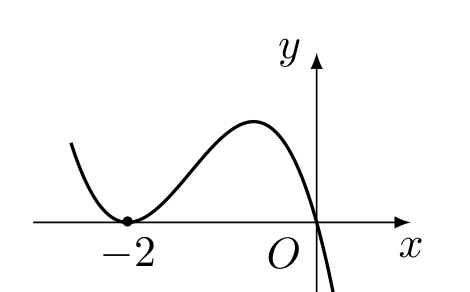
\includegraphics[width=0.15\paperwidth]{GaoKao/images/2012/chongqing_liberal/q8_optA.png}  &  \text{B. }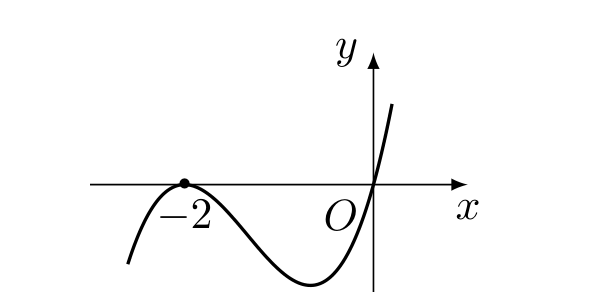
\includegraphics[width=0.15\paperwidth]{GaoKao/images/2012/chongqing_liberal/q8_optB.png}  &  \text{C. }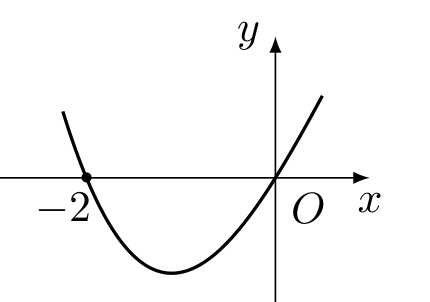
\includegraphics[width=0.15\paperwidth]{GaoKao/images/2012/chongqing_liberal/q8_optC.png}  &  \text{D. }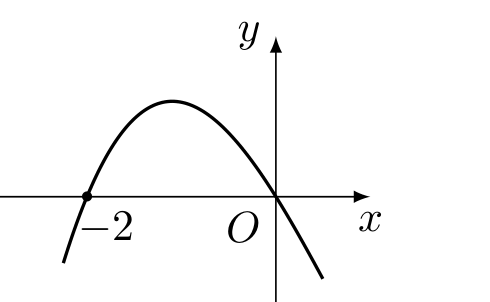
\includegraphics[width=0.15\paperwidth]{GaoKao/images/2012/chongqing_liberal/q8_optD.png}
        \end{tabular*}\par}

        \item 设四面体的六条棱的长分别为 \(1\)，\(1\)，\(1\)，\(1\)，\(\sqrt{2}\) 和 \(a\)，且长为 \(a\) 的棱与长为 \(\sqrt{2}\) 的棱异面，则 \(a\) 的取值范围是（\quad）

        {\centering\begin{tabular*}{\linewidth}{@{}@{\extracolsep{\fill}}llll@{}}
          \text{A. }\((0,\sqrt{2})\)  &  \text{B. }\((0,\sqrt{3})\)  &  \text{C. }\((1,\sqrt{2})\)  &  \text{D. }\((1,\sqrt{3})\)
        \end{tabular*}\par}

        \item 设函数 \(f(x)=x^2-4x+3\)，\(g(x)=3x-2\)，集合 \(M=\{x\in\mathbb{R}\mid f(g(x))>0\}\)，\(N=\{x\in\mathbb{R}\mid g(x)<2\}\)，则 \(M\cap N\) 为（\quad）

        {\centering\begin{tabular*}{\linewidth}{@{}@{\extracolsep{\fill}}llll@{}}
          \text{A. }\((1,+\infty)\)  &  \text{B. }\((0,1)\)  &  \text{C. }\((-1,1)\)  &  \text{D. }\((-\infty,1)\)
        \end{tabular*}\par}

    \end{enumerate}

\end{description}

\begin{description}

    \item[二、填空题]

    \begin{enumerate}[leftmargin=5pt]

      \addtocounter{enumi}{+10}

        \item 首项为 1，公比为 2 的等比数列的前 \(4\) 项和 \(S_{4}=\rule[-0.3ex]{3em}{0.4pt}\).

        \item 若 \(f(x)=(x+a)(x-4)\) 为偶函数，则实数 \(a=\rule[-0.3ex]{3em}{0.4pt}\).

        \item 设 \(\triangle ABC\) 的内角 \(A\)，\(B\)，\(C\) 的对边分别为 \(a\)，\(b\)，\(c\)，且 \(a=1\)，\(b=2\)，\(\cos C=\frac{1}{4}\)，则 \(\sin B=\rule[-0.3ex]{3em}{0.4pt}\).

        \item 设 \(P\) 为直线 \(y=\frac{b}{3a}x\) 与双曲线 \(\frac{x^2}{a^2}-\frac{y^2}{b^2}=1\) （\(a>0,b>0\)） 左支的交点，\(F_1\) 是左焦点，\(PF_1\) 垂直于 \(x\) 轴，则双曲线的离心率 \(e=\rule[-0.3ex]{3em}{0.4pt}\).

        \item 某艺校在一天的 \(6\) 节课中随机安排语文，数学，外语三门文化课和其他三门艺术课各 \(1\) 节，则在课表上的相邻两节文化课之间至少间隔 \(1\) 节艺术课的概率为\rule[-0.3ex]{3em}{0.4pt}. （用数字作答）

    \end{enumerate}

\end{description}

\begin{description}

    \item[三、解答题]

    \begin{enumerate}[leftmargin=5pt]

      \addtocounter{enumi}{+15}

        \item 已知 \(\{a_{n}\}\) 为等差数列，且 \(a_{1}+a_{3}=8\)，\(a_{2}+a_{4}=12\).

\begin{enumerate}
\item 求 \(\{a_{n}\}\) 的通项公式；
\item 记 \(\{a_{n}\}\) 的前 \(n\) 项和为 \(\{S_{n}\}\)，若 \(a_{1}\)，\(a_{k}\)，\(a_{k+2}\) 成等比数列，求正整数 \(k\) 的值.
\end{enumerate}

        \item 已知函数 \(f(x)=ax^3+bx+c\) 在点 \(x=2\) 处取得极值 \(c-16\).

\begin{enumerate}
\item 求 \(a\)，\(b\) 的值；
\item 若 \(f(x)\) 有极大值 28，求 \(f(x)\) 在 \([-3,3]\) 上的最小值.
\end{enumerate}

        \item 甲，乙两人轮流投篮，每人每次投一球. 约定甲先投且先投中者获胜，一直到有人获胜或每人都已投球 \(3\) 次时投篮结束. 设甲每次投篮投中的概率为 \(\frac{1}{3}\)，乙每次投篮投中的概率为 \(\frac{1}{2}\)，且各次投篮互不影响.

\begin{enumerate}
\item 求乙获胜的概率；
\item 求投篮结束时乙只投了 \(2\) 个球的概率.
\end{enumerate}

        \item 设函数 \(f(x)=A\sin(\omega x+\varphi)\)（其中 \(A>0\)，\(\omega>0\)，\(-\pi<\varphi\leqslant \pi\)）在 \(x=\frac{\pi}{6}\) 处取得最大值 2，其图象与 \(x\) 轴的相邻两个交点的距离为 \(\frac{\pi}{2}\).

\begin{enumerate}
\item 求 \(f(x)\) 的解析式；
\item 求函数 \(g(x)=\frac{6\cos^{4}x-\sin^{2}x-1}{f\left(x+\frac{\pi}{6}\right)}\) 的值域.
\end{enumerate}

        \item 如图，在直三棱柱 \(ABC-A_{1}B_{1}C_{1}\) 中，\(AB=4\)，\(AC=BC=3\)，\(D\) 为 \(AB\) 的中点.

\begin{enumerate}
\item 求异面直线 \(CC_{1}\) 和 \(AB\) 的距离；
\item 若 \(AB_{1}\perp A_{1}C\)，求二面角 \(A_{1}-CD-B_{1}\) 的平面角的余弦值.
\end{enumerate}

\begin{center}
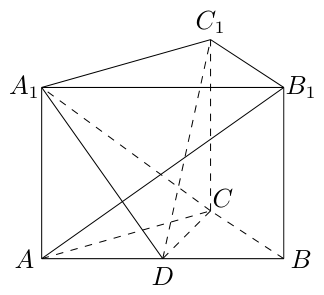
\includegraphics[width=5.7cm]{GaoKao/images/2012/chongqing_liberal/q20_fig1.png}
\end{center}

        \item 如图，设椭圆的中心为原点 \(O\)，长轴在 \(x\) 轴上，上顶点为 \(A\)，左，右焦点分别为 \(F_{1}\)，\(F_{2}\)，线段 \(OF_{1}\)，\(OF_{2}\) 的中点分别为 \(B_{1}\)，\(B_{2}\)，且 \(\triangle AB_{1}B_{2}\) 是面积为 \(4\) 的直角三角形.

\begin{enumerate}
\item 求该椭圆的离心率和标准方程；
\item 过 \(B_{1}\) 作直线交椭圆于 \(P\)，\(Q\) 两点，使 \(PB_{2}\perp QB_{2}\)，求 \(\triangle PB_{2}Q\) 的面积.
\end{enumerate}

\begin{center}
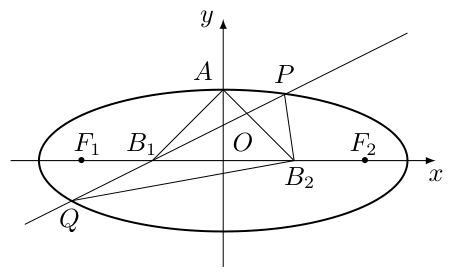
\includegraphics[width=8.2cm]{GaoKao/images/2012/chongqing_liberal/q21_fig1.png}
\end{center}

    \end{enumerate}

\end{description}


\subsection{2012年福建卷（理）}\label{gk:2012年福建卷（理）}

\begin{description}

    \item[一、选择题]

    \begin{enumerate}[leftmargin=5pt]

        \item 若复数 \(z\) 满足 \(z\i = 1 - \i\)，则 \(z\) 等于（\quad）

        {\centering\begin{tabular*}{\linewidth}{@{}@{\extracolsep{\fill}}llll@{}}
          \text{A. }\(-1 - \i\)  &  \text{B. }\(1 - \i\)  &  \text{C. }\(-1 + \i\)  &  \text{D. }\(1 + \i\)
        \end{tabular*}\par}

        \item 等差数列 \(\{a_{n}\}\) 中，\(a_{1} + a_{5} = 10\)，\(a_{4} = 7\)，则数列 \(\{a_{n}\}\) 的公差为（\quad）

        {\centering\begin{tabular*}{\linewidth}{@{}@{\extracolsep{\fill}}llll@{}}
          \text{A. }\(1\)  &  \text{B. }\(2\)  &  \text{C. }\(3\)  &  \text{D. }\(4\)
        \end{tabular*}\par}

        \item 下列命题中，真命题是（\quad）

\begin{enumerate}
\item \(\exists x_{0} \in \mathbb{R}\)，\({\mathrm{e}}^{x_{0}} \leqslant 0\)；
\item \(\forall x \in \mathbb{R}\)，\(2^{x} > x^{2}\)；
\item \(a + b = 0\) 的充要条件是 \(\frac{a}{b} = -1\)；
\item \(a > 1\)，\(b > 1\) 是 \(ab > 1\) 的充分条件.
\end{enumerate}

        {\centering\begin{tabular*}{\linewidth}{@{}@{\extracolsep{\fill}}llll@{}}
          \text{A. }\(\ding{172}\ding{173}\)  &  \text{B. }\(\ding{172}\ding{174}\)  &  \text{C. }\(\ding{173}\ding{175}\)  &  \text{D. }\(\ding{174}\ding{175}\)
        \end{tabular*}\par}

        \item 一个几何体的三视图形状都相同，大小均相等，那么这个几何体不可以是（\quad）

        {\centering\begin{tabular*}{\linewidth}{@{}@{\extracolsep{\fill}}llll@{}}
          \text{A. }球  &  \text{B. }三棱锥  &  \text{C. }正方体  &  \text{D. }圆柱
        \end{tabular*}\par}

        \item 下列不等式一定成立的是（\quad）

        {\centering\begin{tabular*}{\linewidth}{@{}@{\extracolsep{\fill}}llll@{}}
          \text{A. }\(\lg\left(x^{2}+\frac{1}{4}\right) > \lg x\)（\(x > 0\)）  &  \text{B. }\(\sin x + \frac{1}{\sin x} \geqslant 2\)（\(x \neq k\pi\)，\(k \in \mathbb{Z}\)）  &  \text{C. }\(x^{2} + 1 \geqslant 2|x|\)（\(x \in \mathbb{R}\)）  &  \text{D. }\(\frac{1}{x^{2} + 1} > 1\)（\(x \in \mathbb{R}\)）
        \end{tabular*}\par}

        \item 如图所示，在边长为 \(1\) 的正方形 \(OABC\) 中任取一点 \(P\)，则点 \(P\) 恰好取自阴影部分的概率为（\quad）

\begin{center}
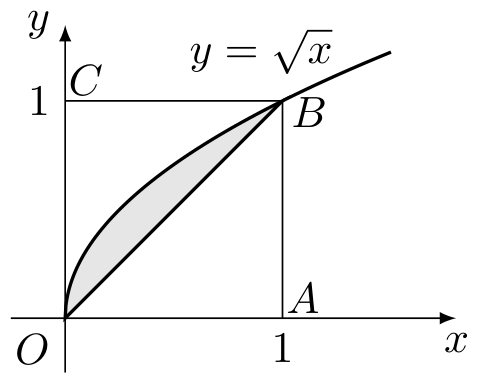
\includegraphics[width=5.9cm]{GaoKao/images/2012/fujian_science/q6_fig1.png}
\end{center}

        {\centering\begin{tabular*}{\linewidth}{@{}@{\extracolsep{\fill}}llll@{}}
          \text{A. }\(\frac{1}{4}\)  &  \text{B. }\(\frac{1}{5}\)  &  \text{C. }\(\frac{1}{6}\)  &  \text{D. }\(\frac{1}{7}\)
        \end{tabular*}\par}

        \item 设函数 \(D(x) = \begin{cases}
1, & x\text{ 为有理数},\\
0, & x\text{ 为无理数},
\end{cases}\) 则下列结论错误的是（\quad）

        {\centering\begin{tabular*}{\linewidth}{@{}@{\extracolsep{\fill}}llll@{}}
          \text{A. }\(D(x)\) 的值域为 \(\{0,1\}\)  &  \text{B. }\(D(x)\) 是偶函数  &  \text{C. }\(D(x)\) 不是周期函数  &  \text{D. }\(D(x)\) 不是单调函数
        \end{tabular*}\par}

        \item 已知双曲线 \(\frac{x^{2}}{4} - \frac{y^{2}}{b^{2}} = 1\) 的右焦点与抛物线 \(y^{2} = 12x\) 的焦点重合，则该双曲线的焦点到其渐近线的距离等于（\quad）

        {\centering\begin{tabular*}{\linewidth}{@{}@{\extracolsep{\fill}}llll@{}}
          \text{A. }\(\sqrt{5}\)  &  \text{B. }\(4\sqrt{2}\)  &  \text{C. }3  &  \text{D. }5
        \end{tabular*}\par}

        \item 若函数 \(y = 2^{x}\) 图象上存在点 \((x,y)\) 满足约束条件 \(\begin{cases}
x + y - 3 \leqslant 0,\\
x - 2y - 3 \leqslant 0,\\
x \geqslant m,
\end{cases}\) 则实数 \(m\) 的最大值为（\quad）

        {\centering\begin{tabular*}{\linewidth}{@{}@{\extracolsep{\fill}}llll@{}}
          \text{A. }\(\frac{1}{2}\)  &  \text{B. }1  &  \text{C. }\(\frac{3}{2}\)  &  \text{D. }2
        \end{tabular*}\par}

        \item 函数 \(f(x)\) 在 \([a,b]\) 上有定义，若对任意 \(x_{1}\)，\(x_{2} \in [a,b]\)，有 \(f\left(\frac{x_{1} + x_{2}}{2}\right) \leqslant \frac{1}{2}[f(x_{1}) + f(x_{2})]\)，则称 \(f(x)\) 在 \([a,b]\) 上具有性质 \(P\). 设 \(f(x)\) 在 \([1,3]\) 上具有性质 \(P\)，现给出如下命题：

\begin{enumerate}
\item \(f(x)\) 在 \([1,3]\) 上的图象是连续不断的；
\item \(f(x^{2})\) 在 \([1,\sqrt{3}]\) 上具有性质 \(P\)；
\item 若 \(f(x)\) 在 \(x = 2\) 处取得最大值 \(1\)，则 \(f(x) = 1\)，\(x \in [1,3]\)；
\item 对任意 \(x_{1}\)，\(x_{2}\)，\(x_{3}\)，\(x_{4} \in [1,3]\)，有 \(f\left(\frac{x_{1} + x_{2} + x_{3} + x_{4}}{4}\right) \leqslant \frac{1}{4}[f(x_{1}) + f(x_{2}) + f(x_{3}) + f(x_{4})]\).
\end{enumerate}

其中真命题的序号是（\quad）

        {\centering\begin{tabular*}{\linewidth}{@{}@{\extracolsep{\fill}}llll@{}}
          \text{A. }\(\ding{172}\ding{173}\)  &  \text{B. }\(\ding{172}\ding{174}\)  &  \text{C. }\(\ding{173}\ding{175}\)  &  \text{D. }\(\ding{174}\ding{175}\)
        \end{tabular*}\par}

    \end{enumerate}

\end{description}

\begin{description}

    \item[二、填空题]

    \begin{enumerate}[leftmargin=5pt]

      \addtocounter{enumi}{+10}

        \item \((a + x)^{4}\) 的展开式中 \(x^{3}\) 的系数等于 \(8\)，则实数 \(a =\)\rule[-0.3ex]{3em}{0.4pt}.

        \item 阅读如图所示的程序框图，运行相应的程序，输出的 \(s\) 值等于\rule[-0.3ex]{3em}{0.4pt}.

\begin{center}
\begin{center}
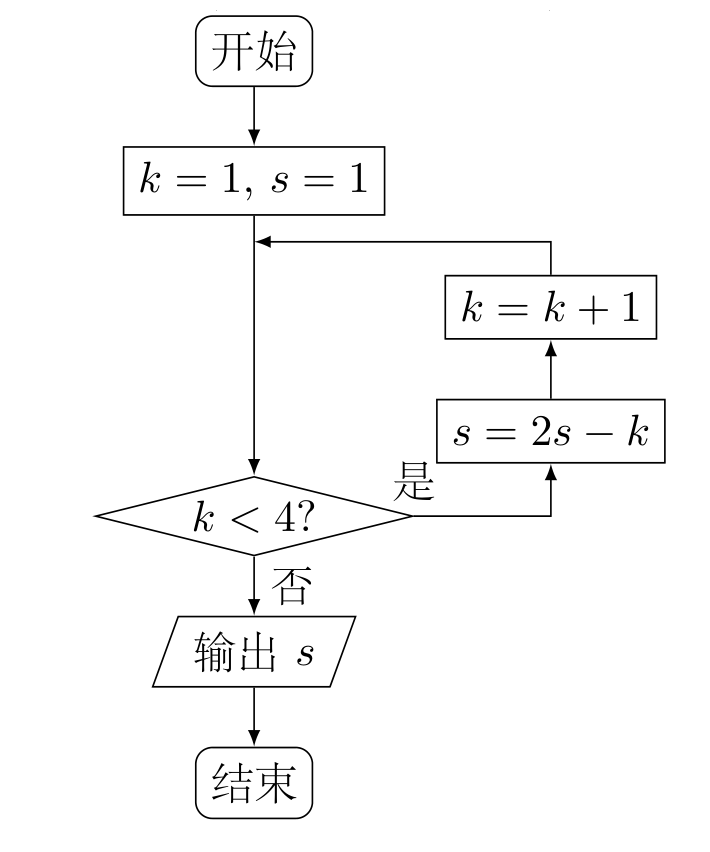
\includegraphics[width=0.44\linewidth]{GaoKao/images/2012/fujian_science/q12_fig1.png}
\end{center}
\end{center}

        \item 已知 \(\triangle ABC\) 的三边长成公比为 \(\sqrt{2}\) 的等比数列，则其最大角的余弦值为\rule[-0.3ex]{3em}{0.4pt}.

        \item 数列 \(\{a_{n}\}\) 的通项公式 \(a_{n} = n\cos\frac{n\pi}{2} + 1\)，前 \(n\) 项和为 \(S_{n}\)，则 \(S_{2012} =\)\rule[-0.3ex]{3em}{0.4pt}.

        \item 对于实数 \(a\) 和 \(b\)，定义运算“\(\ast\)”：\(a \ast b = \begin{cases}
a^{2} - ab, & a \leqslant b,\\
b^{2} - ab, & a > b.
\end{cases}\) 设 \(f(x) = (2x - 1) \ast (x - 1)\)，且关于 \(x\) 的方程 \(f(x) = m\) （\(m \in \mathbb{R}\)）恰有三个互不相等的实数根 \(x_{1}\)，\(x_{2}\)，\(x_{3}\)，则 \(x_{1}x_{2}x_{3}\) 的取值范围是\rule[-0.3ex]{3em}{0.4pt}.

    \end{enumerate}

\end{description}

\begin{description}

    \item[三、解答题]

    \begin{enumerate}[leftmargin=5pt]

      \addtocounter{enumi}{+15}

        \item 受轿车在保修期内维修费等因素的影响，企业生产每辆轿车的利润与该轿车首次出现故障的时间有关. 某轿车制造厂生产甲，乙两种品牌轿车，保修期均为 \(2\) 年. 现从该厂已售出的两种品牌轿车中各随机抽取 \(50\) 辆，统计数据如下：

\begin{center}
\renewcommand{\arraystretch}{1.2}
\begin{tabular}{|c|c|c|c|c|c|}
\hline
品牌 & \multicolumn{3}{c|}{甲} & \multicolumn{2}{c|}{乙} \\
\hline
首次出现故障的时间 \(x\)（\(\text{年}\)） & \(0 < x \leqslant 1\) & \(1 < x \leqslant 2\) & \(x > 2\) & \(0 < x \leqslant 2\) & \(x > 2\) \\
\hline
轿车数量（\(\text{辆}\)） & 2 & 3 & 45 & 5 & 45 \\
\hline
每辆利润（\(\text{万元}\)） & 1 & 2 & 3 & 1.8 & 2.9 \\
\hline
\end{tabular}
\end{center}

将频率视为概率，解答下列问题：

\begin{enumerate}
\item 从该厂生产的甲品牌轿车中随机抽取一辆，求其首次出现故障发生在保修期内的概率；
\item 若该厂生产的轿车均能售出，记生产一辆甲品牌轿车的利润为 \(X_{1}\)，生产一辆乙品牌轿车的利润为 \(X_{2}\)，分别求 \(X_{1}\)，\(X_{2}\) 的分布列；
\item 该厂预计今后这两种品牌轿车销量相当，由于资金限制，只能生产其中一种品牌的新车. 若从经济效益的角度考虑，你认为应生产哪种品牌的轿车？请说明理由.
\end{enumerate}

        \item 某同学在一次研究性学习中发现，以下五个式子的值都等于同一个常数：

\begin{enumerate}
\item \(\sin^{2}13^{\circ} + \cos^{2}17^{\circ} - \sin13^{\circ}\cos17^{\circ}\)；
\item \(\sin^{2}15^{\circ} + \cos^{2}15^{\circ} - \sin15^{\circ}\cos15^{\circ}\)；
\item \(\sin^{2}18^{\circ} + \cos^{2}12^{\circ} - \sin18^{\circ}\cos12^{\circ}\)；
\item \(\sin^{2}(-18^{\circ}) + \cos^{2}48^{\circ} - \sin(-18^{\circ})\cos48^{\circ}\)；
\item \(\sin^{2}(-25^{\circ}) + \cos^{2}55^{\circ} - \sin(-25^{\circ})\cos55^{\circ}\).
\end{enumerate}

\begin{enumerate}
\item 试从上述五个式子中选择一个，求出这个常数；
\item 根据（1）的计算结果，将该同学的发现推广为三角恒等式，并证明你的结论.
\end{enumerate}

        \item 如图，在长方体 \(ABCD-A_{1}B_{1}C_{1}D_{1}\) 中，\(AA_{1} = AD = 1\)，\(E\) 为 \(CD\) 的中点.

\begin{enumerate}
\item 求证：\(B_{1}E \perp AD_{1}\)；
\item 在棱 \(AA_{1}\) 上是否存在一点 \(P\)，使得 \(DP \parallel\) 平面 \(B_{1}AE\)？若存在，求 \(AP\) 的长；若不存在，请说明理由；
\item 若二面角 \(A-B_{1}E-A_{1}\) 的大小为 \(30^{\circ}\)，求 \(AB\) 的长.
\end{enumerate}

\begin{center}
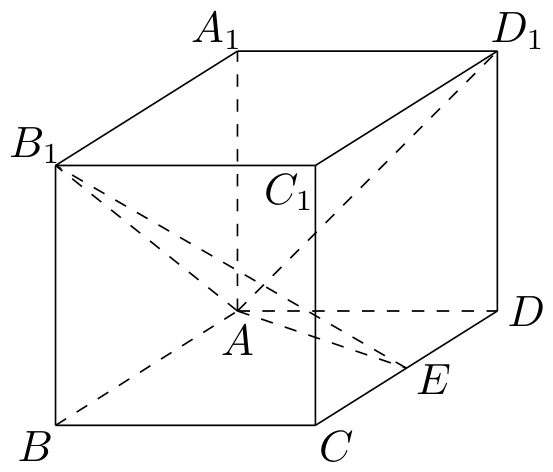
\includegraphics[width=5.5cm]{GaoKao/images/2012/fujian_science/q18_fig1.png}
\end{center}

        \item 如图，椭圆 \(E: \frac{x^{2}}{a^{2}} + \frac{y^{2}}{b^{2}} = 1\)（\(a > b > 0\)）的左焦点为 \(F_{1}\)，右焦点为 \(F_{2}\)，离心率 \(\varepsilon = \frac{1}{2}\)，过 \(F_{1}\) 的直线交椭圆于 \(A\)，\(B\) 两点，且 \(\triangle ABF_{2}\) 的周长为 \(8\).

\begin{enumerate}
\item 求椭圆 \(E\) 的方程；
\item 设动直线 \(l: y = kx + m\) 与椭圆 \(E\) 有且只有一个公共点 \(P\)，且与直线 \(x = 4\) 相交于点 \(Q\). 试探究：在坐标平面内是否存在定点 \(M\)，使得以 \(PQ\) 为直径的圆恒过点 \(M\)？若存在，求出点 \(M\) 的坐标；若不存在，请说明理由.
\end{enumerate}

\begin{center}
\begin{center}
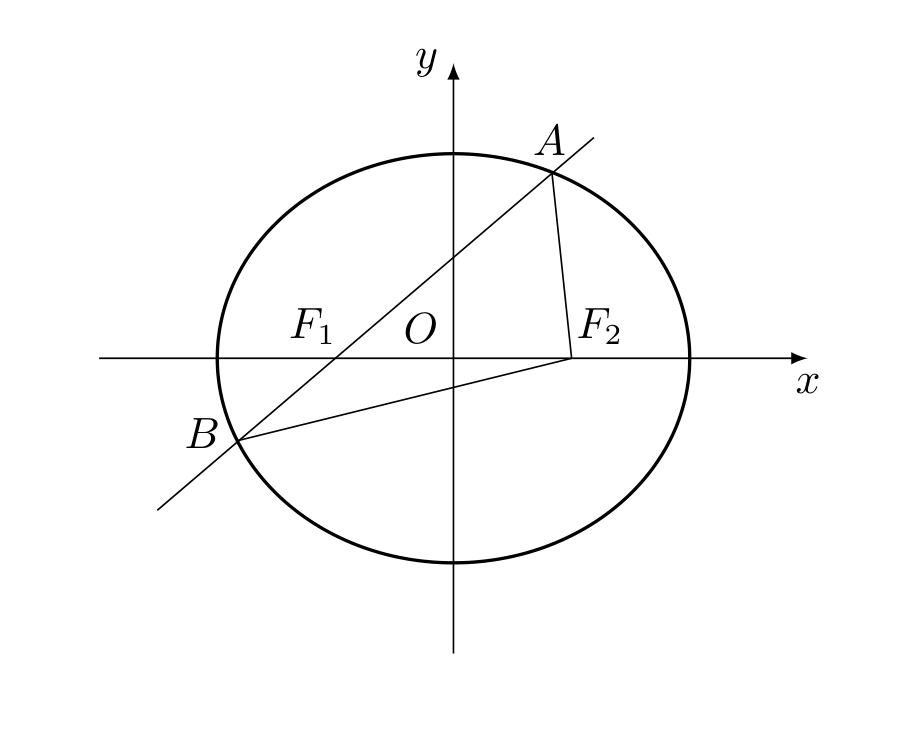
\includegraphics[width=9.5cm]{GaoKao/images/2012/fujian_science/q19_fig1.png}
\end{center}
\end{center}

        \item 已知函数 \(f(x) = {\mathrm{e}}^{x} + ax^{2} - {\mathrm{e}} x\)，\(a \in \mathbb{R}\).

\begin{enumerate}
\item 若曲线 \(y = f(x)\) 在点 \((1,f(1))\) 处的切线平行于 \(x\) 轴，求函数 \(f(x)\) 的单调区间；
\item 试确定 \(a\) 的取值范围，使得曲线 \(y = f(x)\) 上存在唯一的点 \(P\)，曲线在该点处的切线与曲线只有一个公共点 \(P\).
\end{enumerate}

    \end{enumerate}

\end{description}

\begin{description}

    \item[四、选考题]

    \begin{enumerate}[leftmargin=5pt]

      \addtocounter{enumi}{+20}

        \item 设曲线 \(2x^{2} + 2xy + y^{2} = 1\) 在矩阵 \(\mathbf{A} = \begin{pmatrix} a & 0 \\ b & 1 \end{pmatrix}\) （\(a > 0\)）对应的变换作用下得到的曲线为 \(x^{2} + y^{2} = 1\).

\begin{enumerate}
\item 求实数 \(a\)，\(b\) 的值；
\item 求 \(A^{2}\) 的逆矩阵.
\end{enumerate}

        \item \textbf{【选修4-4：坐标系与参数方程】}

在平面直角坐标系中，以坐标原点 \(O\) 为极点，\(x\) 轴的正半轴为极轴建立极坐标系. 已知直线 \(l\) 上两点 \(M\)，\(N\) 的极坐标分别为 \((2,0)\)，\(\left(\frac{2\sqrt{3}}{3},\frac{\pi}{2}\right)\)，圆 \(C\) 的参数方程为 \(\begin{cases}
x = 2 + 2\cos\theta,\\
y = -\sqrt{3} + 2\sin\theta,
\end{cases}\)（\(\theta\) 为参数）.

\begin{enumerate}
\item 设 \(P\) 为线段 \(MN\) 的中点，求直线 \(OP\) 的平面直角坐标方程；
\item 判断直线 \(l\) 与圆 \(C\) 的位置关系.
\end{enumerate}

        \item 已知函数 \(f(x) = m - |x - 2|\)，\(m \in \mathbb{R}\). 且 \(f(x + 2) \geqslant 0\) 的解集为 \([-1,1]\).

\begin{enumerate}
\item 求 \(m\) 的值；
\item 若 \(a\)，\(b\)，\(c \in \mathbb{R}^{+}\)，且 \(\frac{1}{a} + \frac{1}{2b} + \frac{1}{3c} = m\)，求证：\(a + 2b + 3c \geqslant 9\).
\end{enumerate}

    \end{enumerate}

\end{description}


\subsection{2012年福建卷（文）}\label{gk:2012年福建卷（文）}

\begin{description}

    \item[一、选择题]

    \begin{enumerate}[leftmargin=5pt]

        \item 复数 \((2 + \i)^2\) 等于（\quad）

        {\centering\begin{tabular*}{\linewidth}{@{}@{\extracolsep{\fill}}llll@{}}
          \text{A. }\(3 + 4\i\)  &  \text{B. }\(5 + 4\i\)  &  \text{C. }\(3 + 2\i\)  &  \text{D. }\(5 + 2\i\)
        \end{tabular*}\par}

        \item 已知集合 \(M = \{1, 2, 3, 4\}\)，\(N = \{-2, 2\}\)，下列结论成立的是（\quad）

        {\centering\begin{tabular*}{\linewidth}{@{}@{\extracolsep{\fill}}llll@{}}
          \text{A. }\(N \subseteq M\)  &  \text{B. }\(M \cup N = M\)  &  \text{C. }\(M \cap N = N\)  &  \text{D. }\(M \cap N = \{2\}\)
        \end{tabular*}\par}

        \item 已知向量 \(\bm{a} = (x - 1, 2)\)，\(\bm{b} = (2, 1)\)，则 \(\bm{a} \perp \bm{b}\) 的充要条件是（\quad）

        {\centering\begin{tabular*}{\linewidth}{@{}@{\extracolsep{\fill}}llll@{}}
          \text{A. }\(x = -\frac{1}{2}\)  &  \text{B. }\(x = -1\)  &  \text{C. }\(x = 5\)  &  \text{D. }\(x = 0\)
        \end{tabular*}\par}

        \item 一个几何体的三视图形状都相同、大小均相等，那么这个几何体不可以是（\quad）

        {\centering\begin{tabular*}{\linewidth}{@{}@{\extracolsep{\fill}}llll@{}}
          \text{A. }球  &  \text{B. }三棱锥  &  \text{C. }正方体  &  \text{D. }圆柱
        \end{tabular*}\par}

        \item 已知双曲线 \(\frac{x^2}{a^2} - \frac{y^2}{5} = 1\) 的右焦点为\((3,0)\)，则该双曲线的离心率等于（\quad）

        {\centering\begin{tabular*}{\linewidth}{@{}@{\extracolsep{\fill}}llll@{}}
          \text{A. }\(\frac{3\sqrt{14}}{14}\)  &  \text{B. }\(\frac{3\sqrt{2}}{4}\)  &  \text{C. }\(\frac{3}{2}\)  &  \text{D. }\(\frac{4}{3}\)
        \end{tabular*}\par}

        \item 阅读如图所示的程序框图，运行相应的程序，输出的 \(s\) 值等于（\quad）

\begin{center}
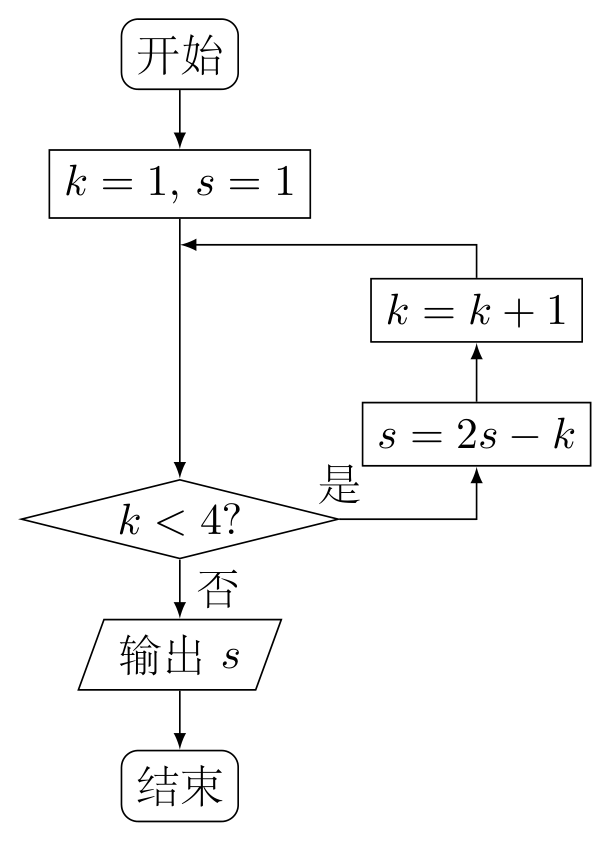
\includegraphics[width=0.34\linewidth]{GaoKao/images/2012/fujian_liberal/q6_fig1.png}
\end{center}

        {\centering\begin{tabular*}{\linewidth}{@{}@{\extracolsep{\fill}}llll@{}}
          \text{A. }\(-3\)  &  \text{B. }\(-10\)  &  \text{C. }\(0\)  &  \text{D. }\(-2\)
        \end{tabular*}\par}

        \item 直线 \(x + \sqrt{3} y - 2 = 0\) 与圆 \(x^{2} + y^{2} = 4\) 相交于 \(A\)，\(B\) 两点，则弦 \(AB\) 的长度等于（\quad）

        {\centering\begin{tabular*}{\linewidth}{@{}@{\extracolsep{\fill}}llll@{}}
          \text{A. }\(2 \sqrt{5}\)  &  \text{B. }\(2 \sqrt{3}\)  &  \text{C. }\(\sqrt{3}\)  &  \text{D. }\(1\)
        \end{tabular*}\par}

        \item 函数 \( f(x) = \sin \left(x - \frac{\pi}{4}\right) \) 的图象的一条对称轴是（\quad）

        {\centering\begin{tabular*}{\linewidth}{@{}@{\extracolsep{\fill}}llll@{}}
          \text{A. }\(x = \frac{\pi}{4}\)  &  \text{B. }\(x = \frac{\pi}{2}\)  &  \text{C. }\(x = -\frac{\pi}{4}\)  &  \text{D. }\(x = -\frac{\pi}{2}\)
        \end{tabular*}\par}

        \item 设 \(f(x) = \begin{cases}
1, & x > 0,\\
0, & x = 0,\\
-1, & x < 0,
\end{cases}
\qquad g(x) = \begin{cases}
1, & x \text{为有理数},\\
0, & x \text{为无理数},
\end{cases}\)
则 \(f(g(\pi))\) 的值为（\quad）

        {\centering\begin{tabular*}{\linewidth}{@{}@{\extracolsep{\fill}}llll@{}}
          \text{A. }\(1\)  &  \text{B. }\(0\)  &  \text{C. }\(-1\)  &  \text{D. }\(\pi\)
        \end{tabular*}\par}

        \item 若直线 \( y = 2x \) 上存在点 \((x, y)\) 满足约束条件 \(\begin{cases}
x + y - 3 \leqslant 0,\\
x - 2y - 3 \leqslant 0,\\
x \geqslant m.
\end{cases}\) 则实数 \( m \) 的最大值为（\quad）

        {\centering\begin{tabular*}{\linewidth}{@{}@{\extracolsep{\fill}}llll@{}}
          \text{A. }\(-1\)  &  \text{B. }\(1\)  &  \text{C. }\( \frac{3}{2} \)  &  \text{D. }\(2\)
        \end{tabular*}\par}

        \item 数列 \(\{a_{n}\}\) 的通项公式 \(a_{n} = n\cos \frac{n\pi}{2}\)，其前 \(n\) 项和为 \(S_{n}\)，则 \(S_{2012}\) 等于（\quad）

        {\centering\begin{tabular*}{\linewidth}{@{}@{\extracolsep{\fill}}llll@{}}
          \text{A. }\(1006\)  &  \text{B. }\(2012\)  &  \text{C. }\(503\)  &  \text{D. }\(0\)
        \end{tabular*}\par}

        \item 已知 \(f(x)=x^{3}-6x^{2}+9x-abc\)，\(a<b<c\)，且 \( f(a)=f(b)=f(c)=0 \). 现给出如下结论：
\begin{enumerate}
\item \( f(0)f(1)>0 \)；
\item \( f(0)f(1)<0 \)；
\item \( f(0)f(3)>0 \)；
\item \( f(0)f(3)<0 \).
\end{enumerate}
其中正确结论的序号是（\quad）

        {\centering\begin{tabular*}{\linewidth}{@{}@{\extracolsep{\fill}}llll@{}}
          \text{A. }\ding{172}\ding{174}  &  \text{B. }\ding{172}\ding{175}  &  \text{C. }\ding{173}\ding{174}  &  \text{D. }\ding{173}\ding{175}
        \end{tabular*}\par}

    \end{enumerate}

\end{description}

\begin{description}

    \item[二、填空题]

    \begin{enumerate}[leftmargin=5pt]

      \addtocounter{enumi}{+12}

        \item 在 \(\triangle ABC\) 中，已知 \(\angle BAC = 60^{\circ}\)，\(\angle ABC = 45^{\circ}\)，\(BC = \sqrt{3}\)，则 \(AC =\)\rule[-0.3ex]{3em}{0.4pt}.

        \item 一支田径队有男女运动员 \(98\text{ 人}\)，其中男运动员有 \(56\text{ 人}\). 按男女比例用分层抽样的方法，从全体运动员中抽出一个容量为 \(28\) 的样本，那么应抽取女运动员人数是\rule[-0.3ex]{3em}{0.4pt}.

        \item 已知关于 \(x\) 的不等式 \(x^{2} - ax + 2a > 0\) 在 \(\mathbb{R}\) 上恒成立，则实数 \(a\) 的取值范围是\rule[-0.3ex]{3em}{0.4pt}.

        \item 某地区规划道路建设，考虑道路铺设方案；方案设计图中，点表示城市，两点之间连线表示两城市间可铺设道路，连线上数据表示两城市间铺设道路的费用；要求从任一城市都能到达其余各城市，并且铺设道路的总费用最小；例如：在三个城市道路设计中，若城市间可铺设道路的线路图如图 1，则最优设计方案如图 2；此时铺设道路的最小总费用为 10. 现给出该地区可铺设道路的线路图如图 3，则铺设道路的最小总费用为\rule[-0.3ex]{3em}{0.4pt}.

\begin{center}
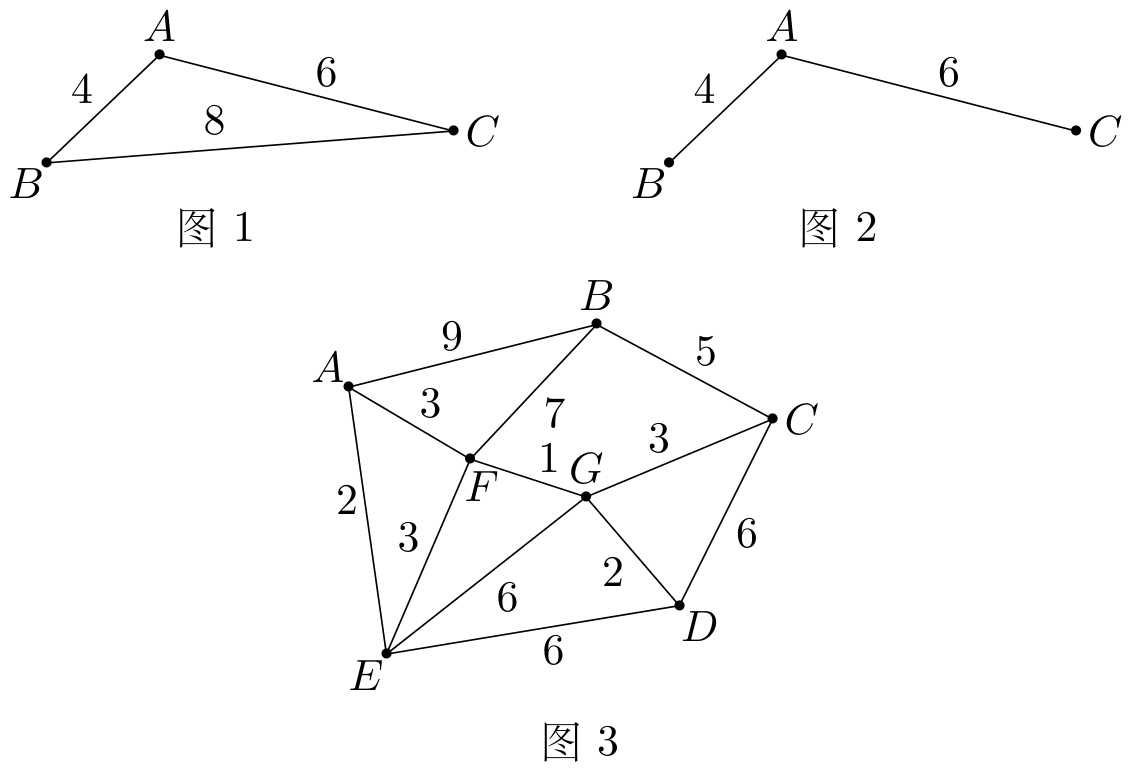
\includegraphics[width=11.2cm]{GaoKao/images/2012/fujian_liberal/q16_fig1.png}
\end{center}

    \end{enumerate}

\end{description}

\begin{description}

    \item[三、解答题]

    \begin{enumerate}[leftmargin=5pt]

      \addtocounter{enumi}{+16}

        \item 在等差数列 \(\{a_{n}\}\) 和等比数列 \(\{b_{n}\}\) 中，\(a_{1} = b_{1} = 1\)，\(b_{4} = 8\)，\(\{a_{n}\}\) 的前 10 项和 \(S_{10} = 55\).
\begin{enumerate}
\item 求 \(a_{n}\) 和 \(b_{n}\)；
\item 现分别从 \( \{a_{n}\} \) 和 \( \{b_{n}\} \) 的前 3 项中各随机抽取一项，写出相应的基本事件，并求这两项的值相等的概率.
\end{enumerate}

        \item 某工厂为了对新研发的一种产品进行合理定价，将该产品按事先拟定的价格进行试销，得到如下数据：
\begin{center}
\begin{tabular}{ccccccc}
单价 \(x\)（\(\text{元}\)） & \(8\) & \(8.2\) & \(8.4\) & \(8.6\) & \(8.8\) & \(9\) \\
销量 \(y\)（\(\text{件}\)） & \(90\) & \(84\) & \(83\) & \(80\) & \(75\) & \(68\)
\end{tabular}
\end{center}
\begin{enumerate}
\item 求回归直线方程 \( \hat{y} = bx + a \)，其中 \(b = -20\)， \( a = \overline{y} - b\overline{x} \)；
\item 预计在今后的销售中，销量与单价仍然服从（1）中的关系，且该产品的成本是\(4\text{ 元/件}\)，为使工厂获得最大利润，该产品的单价应定为多少\(\text{元}\)？（\(\text{利润}=\text{销售收入}-\text{成本}\)）
\end{enumerate}

        \item 如图，在长方体 \(ABCD - A_{1}B_{1}C_{1}D_{1}\) 中，\(AB = AD = 1\)，\(AA_{1} = 2\)，\(M\) 为棱 \(DD_{1}\) 上的一点.
\begin{enumerate}
\item 求三棱锥 \( A - MCC_{1} \) 的体积；
\item 当 \(A_{1}M + MC\) 取得最小值时，求证： \(B_{1}M \perp\) 平面 \(MAC\).
\end{enumerate}

\begin{center}
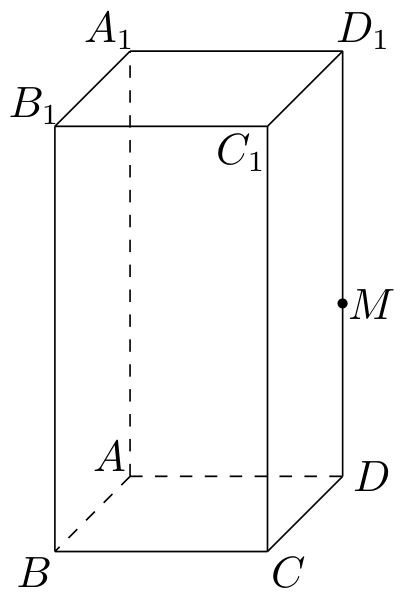
\includegraphics[width=4.0cm]{GaoKao/images/2012/fujian_liberal/q19_fig1.png}
\end{center}

        \item 某同学在一次研究性学习中发现，以下五个式子的值都等于同一个常数：
\begin{enumerate}
\item \( \sin^{2}13^{\circ}+\cos^{2}17^{\circ}-\sin13^{\circ}\cos17^{\circ} \)；
\item \( \sin^{2}15^{\circ}+\cos^{2}15^{\circ}-\sin15^{\circ}\cos15^{\circ} \)；
\item \( \sin^{2}18^{\circ}+\cos^{2}12^{\circ}-\sin18^{\circ}\cos12^{\circ} \)；
\item \( \sin^{2}(-18^{\circ})+\cos^{2}48^{\circ}-\sin(-18^{\circ})\cos48^{\circ} \)；
\item \( \sin^{2}(-25^{\circ})+\cos^{2}55^{\circ}-\sin(-25^{\circ})\cos55^{\circ} \).
\end{enumerate}

\begin{enumerate}
\item 试从上述五个式子中选择一个，求出这个常数；
\item 根据（1）的计算结果，将该同学的发现推广为三角恒等式，并证明你的结论.
\end{enumerate}

        \item 如图，等边三角形 \(OAB\) 的边长为 \(8\sqrt{3}\)，且其三个顶点均在抛物线 \(E: x^{2} = 2py\)（\(p > 0\)）上.
\begin{enumerate}
\item 求抛物线 \(E\) 的方程；
\item 设动直线 \(l\) 与抛物线 \(E\) 相切于点 \(P\)，与直线 \(y=-1\) 相交于点 \(Q\)；证明：以 \(PQ\) 为直径的圆恒过 \(y\) 轴上某定点.
\end{enumerate}

\begin{center}
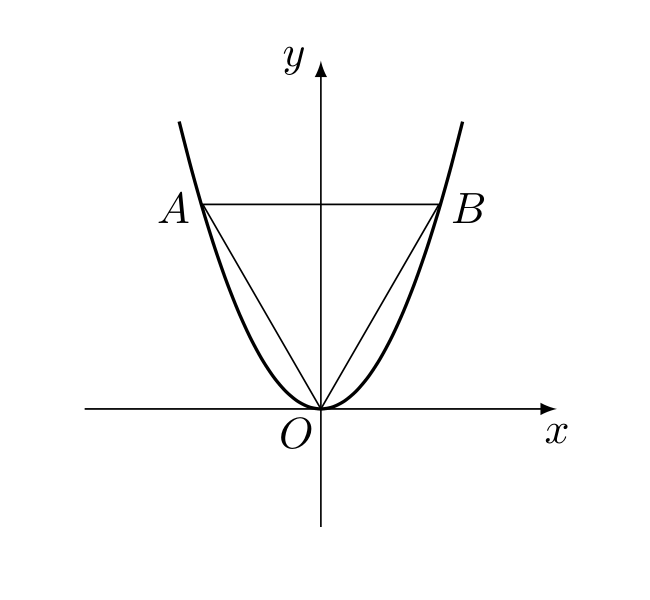
\includegraphics[width=7.1cm]{GaoKao/images/2012/fujian_liberal/q21_fig1.png}
\end{center}

        \item 已知函数 \( f(x) = ax \sin x - \frac{3}{2} \)，\(a \in \mathbb{R}\)，且在 \([0, \frac{\pi}{2}]\) 上的最大值为 \(\frac{\pi - 3}{2}\).
\begin{enumerate}
\item 求函数 \( f(x) \) 的解析式；
\item 判断函数 \( f(x) \) 在 \( (0, \pi) \) 内的零点个数，并加以证明.
\end{enumerate}

    \end{enumerate}

\end{description}


\subsection{2012年广东卷（理）}\label{gk:2012年广东卷（理）}

\begin{description}

    \item[一、选择题]

    \begin{enumerate}[leftmargin=5pt]

        \item 设 \(\i\) 为虚数单位，则复数 \(\frac{5 - 6\i}{\i}=\)（\quad）

        {\centering\begin{tabular*}{\linewidth}{@{}@{\extracolsep{\fill}}llll@{}}
          \text{A. }\(6 + 5\i\)  &  \text{B. }\(6 - 5\i\)  &  \text{C. }\(-6 + 5\i\)  &  \text{D. }\(-6 - 5\i\)
        \end{tabular*}\par}

        \item 设集合 \(U = \{1, 2, 3, 4, 5, 6\}\)，\(M = \{1, 2, 4\}\)，则 \(\complement_U M =\)（\quad）

        {\centering\begin{tabular*}{\linewidth}{@{}@{\extracolsep{\fill}}llll@{}}
          \text{A. }\(U\)  &  \text{B. }\(\{1, 3, 5\}\)  &  \text{C. }\(\{3, 5, 6\}\)  &  \text{D. }\(\{2, 4, 6\}\)
        \end{tabular*}\par}

        \item 若向量 \(\overrightarrow{BA} = (2, 3)\)，\(\overrightarrow{CA} = (4, 7)\)，则 \(\overrightarrow{BC} =\)（\quad）

        {\centering\begin{tabular*}{\linewidth}{@{}@{\extracolsep{\fill}}llll@{}}
          \text{A. }\((-2, -4)\)  &  \text{B. }\((3, 4)\)  &  \text{C. }\((6, 10)\)  &  \text{D. }\((-6, -10)\)
        \end{tabular*}\par}

        \item 下列函数中，在区间 \((0,+\infty)\) 上为增函数的是（\quad）

        {\centering\begin{tabular*}{\linewidth}{@{}@{\extracolsep{\fill}}llll@{}}
          \text{A. }\(y = \ln (x + 2)\)  &  \text{B. }\(y = -\sqrt{x + 1}\)  &  \text{C. }\(y = \left(\frac{1}{2}\right)^x\)  &  \text{D. }\(y = x + \frac{1}{x}\)
        \end{tabular*}\par}

        \item 已知变量 \(x\)，\(y\) 满足约束条件 \(\begin{cases}
y \le 2,\\
x + y \ge 1,\\
x - y \le 1,
\end{cases}\) 则 \(z = 3x + y\) 的最大值为（\quad）

        {\centering\begin{tabular*}{\linewidth}{@{}@{\extracolsep{\fill}}llll@{}}
          \text{A. }\(12\)  &  \text{B. }\(11\)  &  \text{C. }\(3\)  &  \text{D. }\(-1\)
        \end{tabular*}\par}

        \item 某几何体的三视图如图所示，则它的体积为（\quad）

\begin{center}
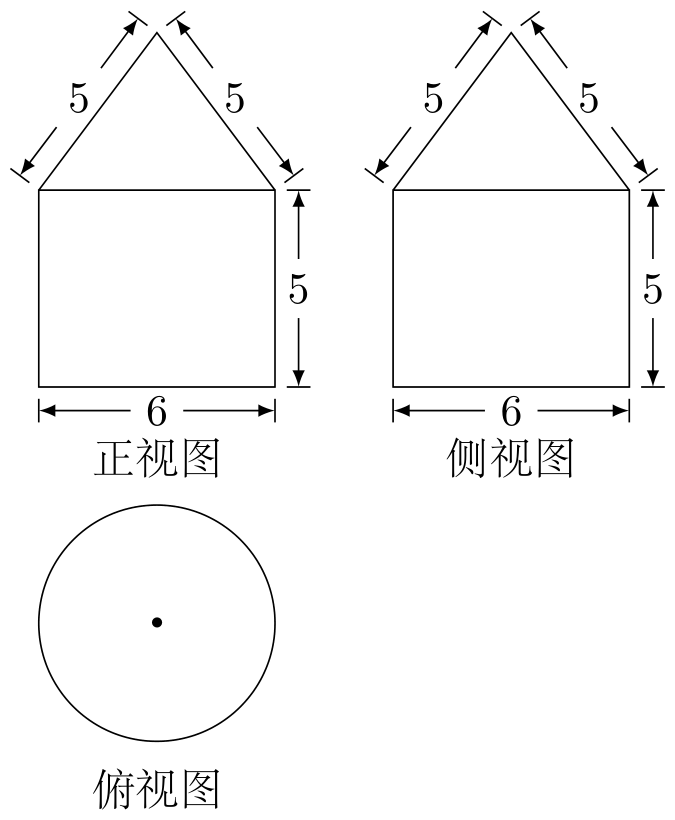
\includegraphics[width=3.6cm]{GaoKao/images/2012/guangdong_science/q6_fig1.png}
\end{center}

        {\centering\begin{tabular*}{\linewidth}{@{}@{\extracolsep{\fill}}llll@{}}
          \text{A. }\(12\pi\)  &  \text{B. }\(45\pi\)  &  \text{C. }\(57\pi\)  &  \text{D. }\(81\pi\)
        \end{tabular*}\par}

        \item 从个位数与十位数之和为奇数的两位数中任取一个，其个位数为 \(0\) 的概率是（\quad）

        {\centering\begin{tabular*}{\linewidth}{@{}@{\extracolsep{\fill}}llll@{}}
          \text{A. }\(\frac{4}{9}\)  &  \text{B. }\(\frac{1}{3}\)  &  \text{C. }\(\frac{2}{9}\)  &  \text{D. }\(\frac{1}{9}\)
        \end{tabular*}\par}

        \item 对任意两个非零的平面向量 \(\bm{\alpha}\) 和 \(\bm{\beta}\)，定义 \(\bm{\alpha} \circ \bm{\beta} = \frac{\bm{\alpha} \cdot \bm{\beta}}{\bm{\beta} \cdot \bm{\beta}}\). 若平面向量 \(\bm{a}\)，\(\bm{b}\) 满足 \(|\bm{a}| \ge |\bm{b}| > 0\)，\(\bm{a}\) 与 \(\bm{b}\) 的夹角 \(\theta \in \left( 0, \frac{\pi}{4} \right)\)，且 \(\bm{a} \circ \bm{b}\) 和 \(\bm{b} \circ \bm{a}\) 都在集合 \(\left\{ \frac{n}{2} \mid n \in \mathbb{Z} \right\}\) 中，则 \(\bm{a} \circ \bm{b} =\)（\quad）

        {\centering\begin{tabular*}{\linewidth}{@{}@{\extracolsep{\fill}}llll@{}}
          \text{A. }\(\frac{1}{2}\)  &  \text{B. }\(1\)  &  \text{C. }\(\frac{3}{2}\)  &  \text{D. }\(\frac{5}{2}\)
        \end{tabular*}\par}

    \end{enumerate}

\end{description}

\begin{description}

    \item[二、填空题]

    \begin{enumerate}[leftmargin=5pt]

      \addtocounter{enumi}{+8}

        \item 不等式 \(|x + 2| - |x| \leqslant 1\) 的解集为\rule[-0.3ex]{3em}{0.4pt}.

        \item \(\left(x^{2} + \frac{1}{x}\right)^{6}\) 的展开式中 \(x^{3}\) 的系数为\rule[-0.3ex]{3em}{0.4pt}. （用数字作答）

        \item 已知递增的等差数列 \(\{a_{n}\}\) 满足 \(a_{1} = 1\)，\(a_{3} = a_{2}^{2} - 4\)，则 \(a_{n} = \)\rule[-0.3ex]{3em}{0.4pt}.

        \item 曲线 \( y = x^{3} - x + 3 \) 在点 \( (1,3) \) 处的切线方程为\rule[-0.3ex]{3em}{0.4pt}.

        \item 执行如图所示的程序框图，若输入 \(n\) 的值为 8，则输出 \(s\) 的值为\rule[-0.3ex]{3em}{0.4pt}.

\begin{center}
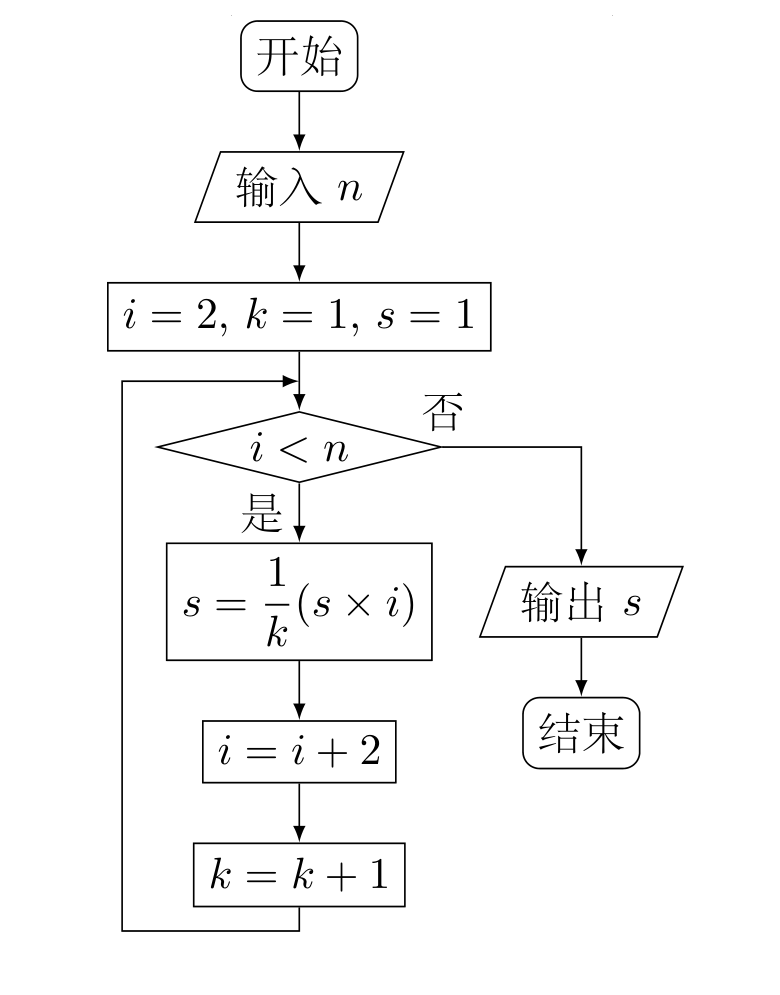
\includegraphics[width=0.38\linewidth]{GaoKao/images/2012/guangdong_science/q13_fig1.png}
\end{center}

    \end{enumerate}

\end{description}

\begin{description}

    \item[三、选考题]

    \begin{enumerate}[leftmargin=5pt]

      \addtocounter{enumi}{+13}

        \item \textbf{【选修4-4：坐标系与参数方程】}

在平面直角坐标系 \(xOy\) 中，曲线 \(C_1\) 和 \(C_2\) 的参数方程分别为 \(\begin{cases}
x = t,\\
y = \sqrt{t},
\end{cases}\) （\(t\) 为参数） 和 \(\begin{cases}
x = \sqrt{2}\cos \theta,\\
y = \sqrt{2}\sin \theta,
\end{cases}\) （\(\theta\) 为参数），则曲线 \(C_1\) 和 \(C_2\) 的交点坐标为\rule[-0.3ex]{3em}{0.4pt}.

        \item \textbf{【选修4-1：几何证明选讲】}

如图，圆 \(O\) 的半径为 \(1\)，\(A\)、\(B\)、\(C\) 是圆周上的三点. 满足 \(\angle ABC = 30^{\circ}\)，过点 \(A\) 作圆 \(O\) 的切线与 \(OC\) 的延长线交于点 \(P\)，则 \(PA =\rule[-0.3ex]{3em}{0.4pt}.\)

\begin{center}
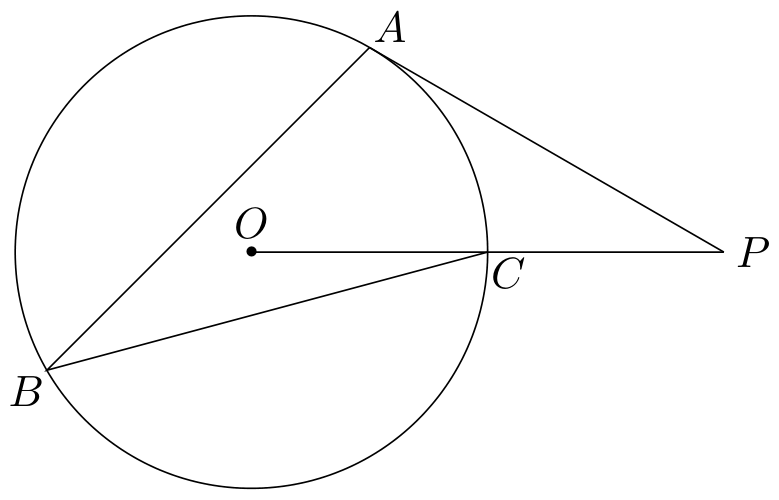
\includegraphics[width=9.1cm]{GaoKao/images/2012/guangdong_science/q15_fig1.png}
\end{center}

    \end{enumerate}

\end{description}

\begin{description}

    \item[四、解答题]

    \begin{enumerate}[leftmargin=5pt]

      \addtocounter{enumi}{+15}

        \item 已知函数 \( f(x) = 2\cos \left( \omega x + \frac{\pi}{6} \right) \) （其中 \(\omega > 0\)，\(x \in \mathbb{R}\) 的最小正周期为 \( 10\pi \)）.
\begin{enumerate}
\item 求 \( \omega \) 的值；
\item 设 \(\alpha\)，\(\beta \in \left[0, \frac{\pi}{2}\right]\)，\( f\left( 5\alpha + \frac{5}{3}\pi \right) = -\frac{6}{5} \)，\( f\left( 5\beta - \frac{5}{6}\pi \right) = \frac{16}{17} \)，求 \( \cos (\alpha + \beta) \) 的值.
\end{enumerate}

        \item 某班 50 位学生期中考试数学成绩的频率分布直方图如图所示，其中成绩分组区间是：\([40,50)\)，\([50,60)\)，\([60,70)\)，\([70,80)\)，\([80,90)\)，\([90,100]\).

\begin{enumerate}
\item 求图中 \(x\) 的值；
\item 从成绩不低于 80 分的学生中随机选取 2 人，该 2 人中成绩在 90 分以上 （含 90 分） 的人数记为 \(\xi\)，求 \(\xi\) 的数学期望.
\end{enumerate}

\begin{center}
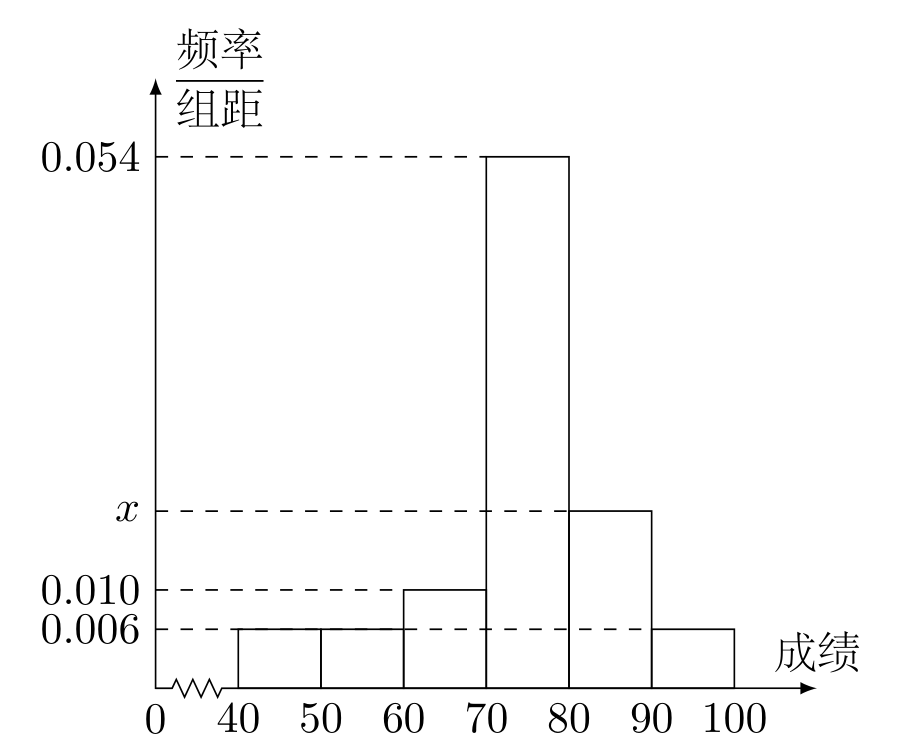
\includegraphics[width=0.62\linewidth]{GaoKao/images/2012/guangdong_science/q17_fig1.png}
\end{center}

        \item 如图所示，在四棱锥 \(P - ABCD\) 中，底面 \(ABCD\) 为矩形，\(PA \perp\) 平面 \(ABCD\)，点 \(E\) 在线段 \(PC\) 上，\(PC \perp\) 平面 \(BDE\).
\begin{enumerate}
\item 证明： \(BD \perp\) 平面 \(PAC\)；
\item 若 \(PA = 1\)，\(AD = 2\)，求二面角 \(B - PC - A\) 的正切值.
\end{enumerate}

\begin{center}
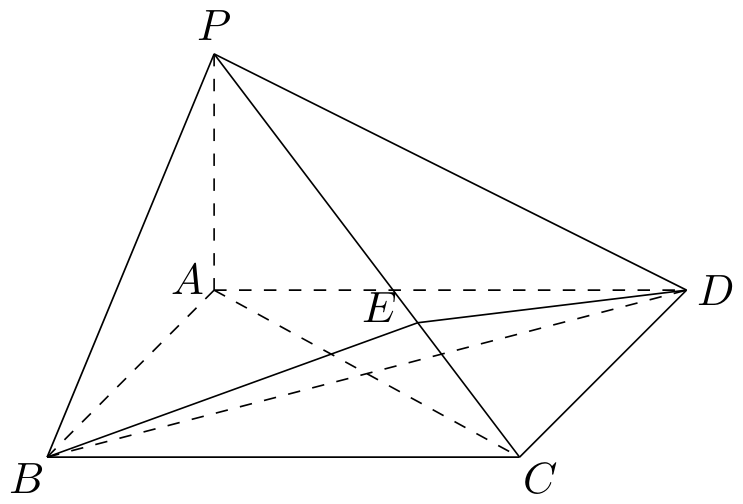
\includegraphics[width=9.2cm]{GaoKao/images/2012/guangdong_science/q18_fig1.png}
\end{center}

        \item 设数列 \(\{a_{n}\}\) 的前 \(n\) 项和为 \(S_{n}\)，满足 \(2S_{n} = a_{n + 1} - 2^{n + 1} + 1\)，\(n \in \mathbf{N}^{*}\)，且 \(a_{1}\)，\(a_{2} + 5\)，\(a_{3}\) 成等差数列.
\begin{enumerate}
\item 求 \(a_{1}\) 的值；
\item 求数列 \(\{a_{n}\}\) 的通项公式；
\item 证明：对一切正整数 \(n\)，有 \(\frac{1}{a_1} + \frac{1}{a_2} + \frac{1}{a_3} + \cdots + \frac{1}{a_n} < \frac{3}{2}\).
\end{enumerate}

        \item 在平面直角坐标系 \(xOy\) 中，已知椭圆 \(C: \frac{x^{2}}{a^{2}} + \frac{y^{2}}{b^{2}} = 1\) （\(a > b > 0\)）的离心率 \(e = \sqrt{\frac{2}{3}}\)，且椭圆 \(C\) 上的点到点 \(Q(0,2)\) 的距离的最大值为 \(3\).
\begin{enumerate}
\item 求椭圆 \(C\) 的方程；
\item 在椭圆 \(C\) 上，是否存在点 \(M(m, n)\)，使得直线 \(l: mx + ny = 1\) 与圆 \(O: x^2 + y^2 = 1\) 相交于不同的两点 \(A\)，\(B\)，且 \(\triangle OAB\) 的面积最大？若存在，求出点 \(M\) 的坐标及相对应的 \(\triangle OAB\) 的面积；若不存在，请说明理由.
\end{enumerate}

        \item 设 \(a < 1\)，集合 \(A = \{x \in \mathbb{R} \mid x > 0\}\)，\(B = \{x \in \mathbb{R} \mid 2x^2 - 3(1 + a)x + 6a > 0\}\)，\(D = A \cap B\).
\begin{enumerate}
\item 求集合 \(D\) （用区间表示）；
\item 求函数 \( f(x) = 2x^3 - 3(1 + a)x^2 + 6ax \) 在 \(D\) 内的极值点.
\end{enumerate}

    \end{enumerate}

\end{description}


\subsection{2012年广东卷（文）}\label{gk:2012年广东卷（文）}

\begin{description}

    \item[一、选择题]

    \begin{enumerate}[leftmargin=5pt]

        \item 设 \(i\) 为虚数单位，则复数 \( \frac{3+4\i}{\i}=\)（\quad）

        {\centering\begin{tabular*}{\linewidth}{@{}@{\extracolsep{\fill}}llll@{}}
          \text{A. }\(-4 - 3\i\)  &  \text{B. }\(-4 + 3\i\)  &  \text{C. }\(4 + 3\i\)  &  \text{D. }\(4 - 3\i\)
        \end{tabular*}\par}

        \item 设集合 \(U = \{1, 2, 3, 4, 5, 6\}\)，\(M = \{1, 3, 5\}\)，则 \(\complement_U M =\)（\quad）

        {\centering\begin{tabular*}{\linewidth}{@{}@{\extracolsep{\fill}}llll@{}}
          \text{A. }\(\{2, 4, 6\}\)  &  \text{B. }\(\{1,3,5\}\)  &  \text{C. }\(\{1,2,4\}\)  &  \text{D. }\(U\)
        \end{tabular*}\par}

        \item 若向量 \(\overrightarrow{AB} = (1, 2)\)，\(\overrightarrow{BC} = (3, 4)\)，则 \(\overrightarrow{AC} =\)（\quad）

        {\centering\begin{tabular*}{\linewidth}{@{}@{\extracolsep{\fill}}llll@{}}
          \text{A. }\((4,6)\)  &  \text{B. }\((-4, -6)\)  &  \text{C. }\((-2, - 2)\)  &  \text{D. }\((2, 2)\)
        \end{tabular*}\par}

        \item 下列函数为偶函数的是（\quad）

        {\centering\begin{tabular*}{\linewidth}{@{}@{\extracolsep{\fill}}llll@{}}
          \text{A. }\(y = \sin x\)  &  \text{B. }\( y = x^{3} \)  &  \text{C. }\(y = {\mathrm{e}}^{x}\)  &  \text{D. }\( y = \ln \sqrt{x^2 + 1} \)
        \end{tabular*}\par}

        \item 已知变量 \(x\)，\(y\) 满足约束条件 \(\begin{cases}
x + y \leqslant 1,\\
x + 1 \geqslant 0,\\
x - y \leqslant 1,
\end{cases}\) 则 \(z = x + 2y\) 的最小值为（\quad）

        {\centering\begin{tabular*}{\linewidth}{@{}@{\extracolsep{\fill}}llll@{}}
          \text{A. }3  &  \text{B. }1  &  \text{C. }\(-5\)  &  \text{D. }\(-6\)
        \end{tabular*}\par}

        \item 在 \(\triangle ABC\) 中，若 \(\angle A = 60^{\circ}\)，\(\angle B = 45^{\circ}\)，\(BC = 3\sqrt{2}\)，则 \(AC =\)（\quad）

        {\centering\begin{tabular*}{\linewidth}{@{}@{\extracolsep{\fill}}llll@{}}
          \text{A. }\(4\sqrt{3}\)  &  \text{B. }\(2\sqrt{3}\)  &  \text{C. }\(\sqrt{3}\)  &  \text{D. }\(\frac{\sqrt{3}}{2}\)
        \end{tabular*}\par}

        \item 某几何体的三视图如图所示，则它的体积为（\quad）

\begin{center}
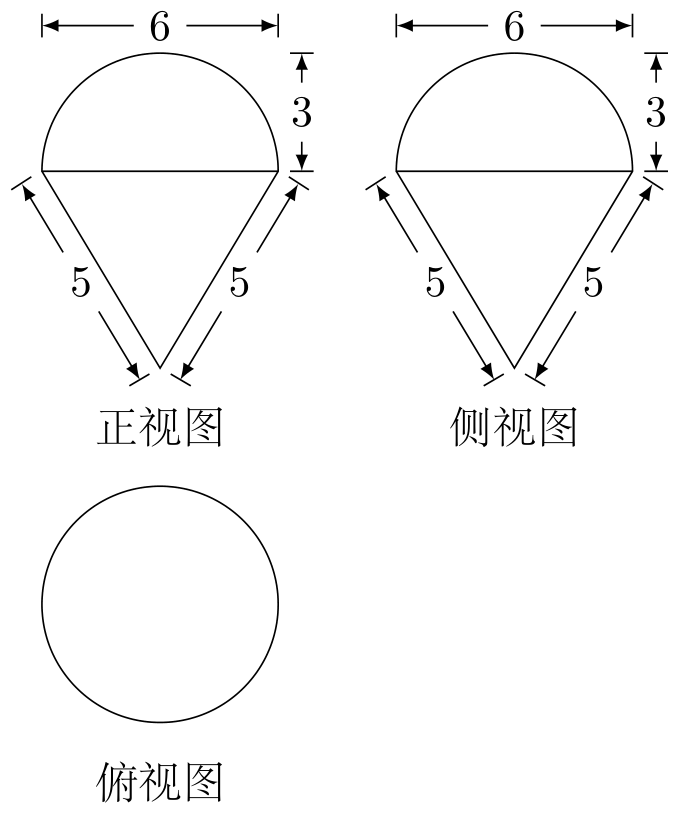
\includegraphics[width=2.1cm]{GaoKao/images/2012/guangdong_liberal/q7_fig1.png}
\end{center}

        {\centering\begin{tabular*}{\linewidth}{@{}@{\extracolsep{\fill}}llll@{}}
          \text{A. }\(72\pi\)  &  \text{B. }\(48\pi\)  &  \text{C. }\(30\pi\)  &  \text{D. }\(24\pi\)
        \end{tabular*}\par}

        \item 在平面直角坐标系 \(xOy\) 中，直线 \(3x + 4y - 5 = 0\) 与圆 \(x^{2} + y^{2} = 4\) 相交于 \(A\)，\(B\) 两点，则弦 \(AB\) 的长等于（\quad）

        {\centering\begin{tabular*}{\linewidth}{@{}@{\extracolsep{\fill}}llll@{}}
          \text{A. }\(3\sqrt{3}\)  &  \text{B. }\(2\sqrt{3}\)  &  \text{C. }\(\sqrt{3}\)  &  \text{D. }1
        \end{tabular*}\par}

        \item 执行如图所示的程序框图，若输入 \(n\) 的值为 6，则输出 \(s\) 的值为（\quad）

\begin{center}
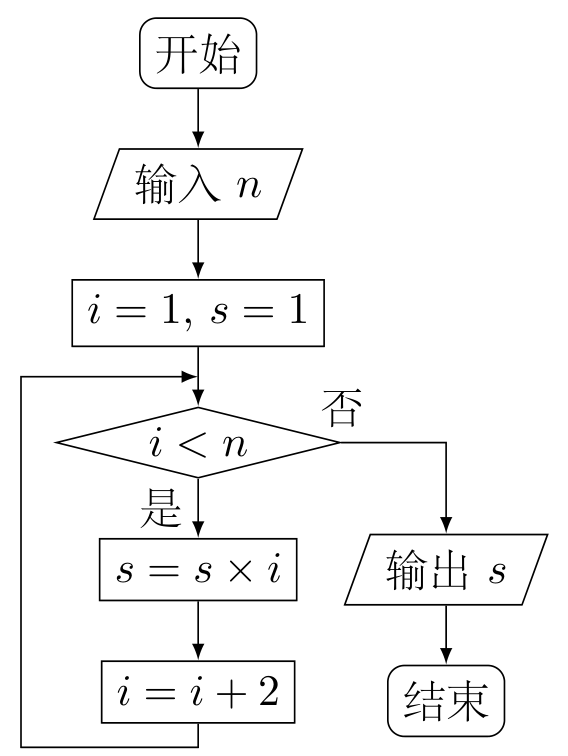
\includegraphics[width=0.30\linewidth]{GaoKao/images/2012/guangdong_liberal/q9_fig1.png}
\end{center}

        {\centering\begin{tabular*}{\linewidth}{@{}@{\extracolsep{\fill}}llll@{}}
          \text{A. }105  &  \text{B. }16  &  \text{C. }15  &  \text{D. }1
        \end{tabular*}\par}

        \item 对任意两个非零的平面向量 \(\bm{\alpha}\) 和 \(\bm{\beta}\)，定义 \(\bm{\alpha} \circ \bm{\beta} = \frac{\bm{\alpha} \cdot \bm{\beta}}{\bm{\beta} \cdot \bm{\beta}}\). 若两个非零的平面向量 \(\bm{a}\)，\(\bm{b}\) 满足 \(\bm{a}\) 与 \(\bm{b}\) 的夹角 \(\theta \in \left(\frac{\pi}{4}, \frac{\pi}{2}\right)\)，且 \(\bm{a} \circ \bm{b}\) 和 \(\bm{b} \circ \bm{a}\) 都在集合 \(\left\{\frac{n}{2} \mid n \in \mathbb{Z}\right\}\) 中，则 \(\bm{a} \circ \bm{b} =\)（\quad）

        {\centering\begin{tabular*}{\linewidth}{@{}@{\extracolsep{\fill}}llll@{}}
          \text{A. }\(\frac{5}{2}\)  &  \text{B. }\(\frac{3}{2}\)  &  \text{C. }1  &  \text{D. }\(\frac{1}{2}\)
        \end{tabular*}\par}

    \end{enumerate}

\end{description}

\begin{description}

    \item[二、填空题]

    \begin{enumerate}[leftmargin=5pt]

      \addtocounter{enumi}{+10}

        \item 函数 \( y = \frac{\sqrt{x + 1}}{x} \) 的定义域为\rule[-0.3ex]{3em}{0.4pt}.

        \item 等比数列 \(\{a_{n}\}\) 满足 \(a_{2}a_{4} = \frac{1}{2}\)，则 \(a_{1}a_{3}^{2}a_{5} =\rule[-0.3ex]{3em}{0.4pt}\).

        \item 由正整数组成的一组数据 \(x_{1}\)，\(x_{2}\)，\(x_{3}\)，\(x_{4}\)，其平均数和中位数都是 2，且标准差等于 1，则这组数据为\rule[-0.3ex]{3em}{0.4pt}. （从小到大排列）

    \end{enumerate}

\end{description}

\begin{description}

    \item[三、选考题]

    \begin{enumerate}[leftmargin=5pt]

      \addtocounter{enumi}{+13}

        \item \textbf{【选修4-4：坐标系与参数方程】}

在平面直角坐标系 \(xOy\) 中，曲线 \(C_1\) 和 \(C_2\) 的参数方程分别为 \(\begin{cases}
x = \sqrt{5} \cos \theta,\\
y = \sqrt{5} \sin \theta,
\end{cases}\) （\(\theta\) 为参数，\(0 \leqslant \theta \leqslant \frac{\pi}{2}\)）和 \(\begin{cases}
x = 1 - \frac{\sqrt{2}}{2} t,\\
y = -\frac{\sqrt{2}}{2} t,
\end{cases}\) （\(t\) 为参数），则曲线 \(C_1\) 与 \(C_2\) 的交点坐标为\rule[-0.3ex]{3em}{0.4pt}.

        \item \textbf{【选修4-1：几何证明选讲】}

如图所示，直线 \(PB\) 与圆 \(O\) 相切于点 \(B\)，\(D\) 是弦 \(AC\) 上的点，\(\angle PBA = \angle DBA\). 若 \(AD = m\)，\(AC = n\)，则 \(AB =\rule[-0.3ex]{3em}{0.4pt}\).

\begin{center}
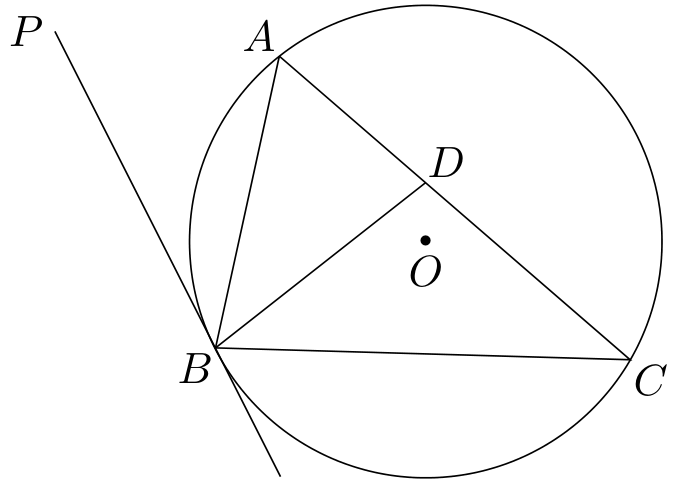
\includegraphics[width=7.9cm]{GaoKao/images/2012/guangdong_liberal/q15_fig1.png}
\end{center}

    \end{enumerate}

\end{description}

\begin{description}

    \item[四、解答题]

    \begin{enumerate}[leftmargin=5pt]

      \addtocounter{enumi}{+15}

        \item 已知函数 \(f(x) = A \cos \left( \frac{x}{4} + \frac{\pi}{6} \right)\)，\(x \in \mathbb{R}\)，且 \( f\left( \frac{\pi}{3} \right) = \sqrt{2} \).
\begin{enumerate}
\item 求 \(A\) 的值；
\item 设 \(\alpha\)，\(\beta \in \left[0, \frac{\pi}{2}\right]\)，\(f\left(4\alpha + \frac{4\pi}{3}\right) = -\frac{30}{17}\)，\(f\left(4\beta - \frac{2\pi}{3}\right) = \frac{8}{5}\)，求 \(\cos (\alpha + \beta)\) 的值.
\end{enumerate}

        \item 某校 100 名学生期中考试语文成绩的频率分布直方图如图所示，其中成绩分组区间是：\([50,60)\)，\([60,70)\)，\([70,80)\)，\([80,90)\)，\([90,100]\).

\begin{enumerate}
\item 求图中 \(a\) 的值；
\item 根据频率分布直方图，估计这 100 名学生语文成绩的平均分；
\item 若这 100 名学生语文成绩某些分数段的人数 \(x\) 与数学成绩相应分数段的人数 \(y\) 之比如下表所示，求数学成绩在 \([50,90)\) 之外的人数.
\begin{center}
{\setlength{\tabcolsep}{7pt}
\begin{tabular}{c|c|c|c|c}
\hline
分数段 & \([50,60)\) & \([60,70)\) & \([70,80)\) & \([80,90)\) \\
\hline
人数比 \(x:y\) & \(1:1\) & \(2:1\) & \(3:4\) & \(4:5\) \\
\hline
\end{tabular}
}
\end{center}
\end{enumerate}

\begin{center}
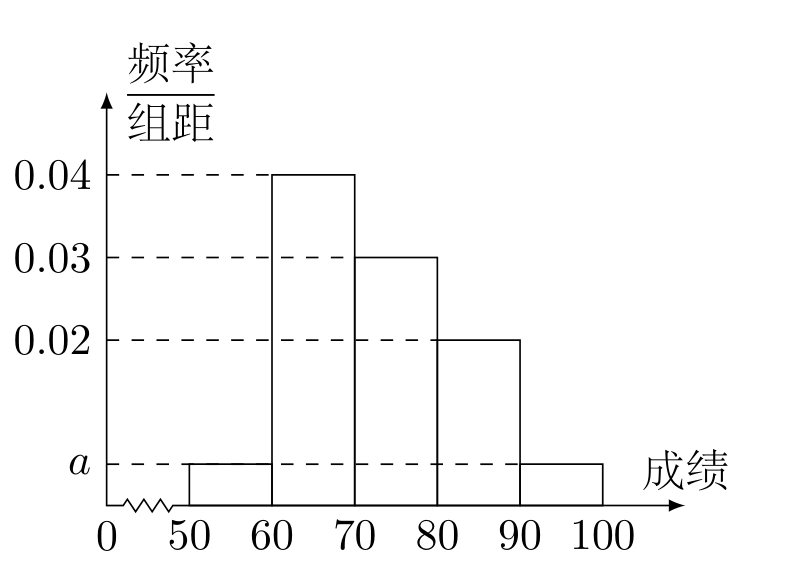
\includegraphics[width=0.60\linewidth]{GaoKao/images/2012/guangdong_liberal/q17_fig1.png}
\end{center}

        \item 如图所示，在四棱锥 \(P - ABCD\) 中，\(AB \perp\) 平面 \(PAD\)，\(AB \parallel CD\)，\(PD = AD\)，\(E\) 是 \(PB\) 中点，\(F\) 是 \(DC\) 上的点且 \(DF = \frac{1}{2} AB\)，\(PH\) 为 \(\triangle PAD\) 中 \(AD\) 边上的高.
\begin{enumerate}
\item 证明： \(PH \perp\) 平面 \(ABCD\)；
\item 若 \(PH = 1\)，\(AD = \sqrt{2}\)，\(FC = 1\)，求三棱锥 \(E - BCF\) 的体积；
\item 证明： \(EF \perp\) 平面 \(PAB\).
\end{enumerate}

\begin{center}
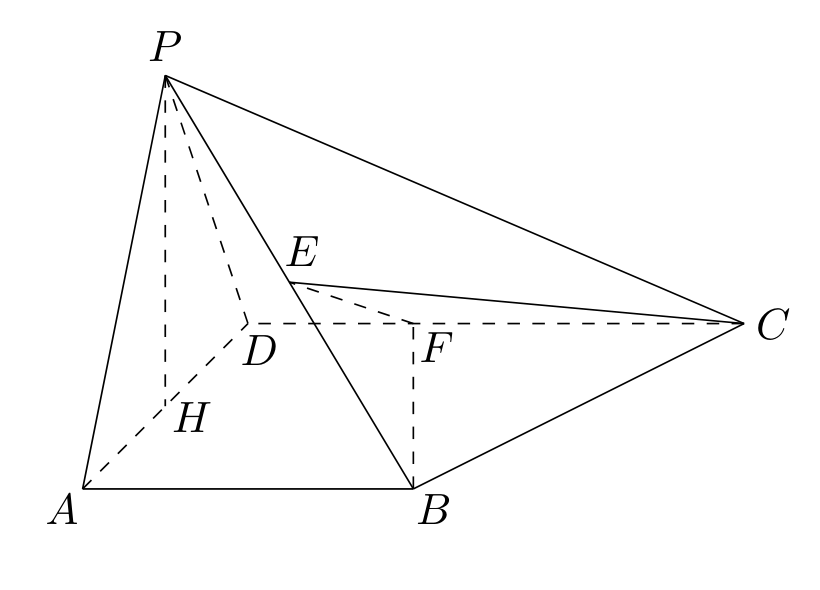
\includegraphics[width=6.5cm]{GaoKao/images/2012/guangdong_liberal/q18_fig1.png}
\end{center}

        \item 设数列 \(\{a_{n}\}\) 的前 \(n\) 项和为 \(S_{n}\). 数列 \(\{S_{n}\}\) 的前 \(n\) 项和为 \(T_{n}\). 满足 \(T_{n} = 2S_{n} - n^{2}\)，\(n \in \mathbf{N}^{*}\).
\begin{enumerate}
\item 求 \(a_{1}\) 的值；
\item 求数列 \(\{a_{n}\}\) 的通项公式.
\end{enumerate}

        \item 在平面直角坐标系 \(xOy\) 中，已知椭圆 \(C_1: \frac{x^2}{a^2} + \frac{y^2}{b^2} = 1\) （\(a > b > 0\)）的左焦点 \(F_1(-1,0)\)，且点 \(P(0,1)\) 在 \(C_1\) 上.
\begin{enumerate}
\item 求椭圆 \(C_1\) 的方程；
\item 设直线 \(l\) 同时为椭圆 \(C_1\) 和抛物线 \(C_2: y^2 = 4x\) 相切，求直线 \(l\) 的方程.
\end{enumerate}

        \item 设 \(0 < a < 1\)，集合 \(A = \{x \in \mathbb{R} \mid x > 0\}\)，\(B = \{x \in \mathbb{R} \mid 2x^2 - 3(1 + a)x + 6a > 0\}\)，\(D = A \cap B\).
\begin{enumerate}
\item 求集合 \(D\) （用区间表示）；
\item 求函数 \( f(x) = 2x^{3} - 3(1 + a)x^{2} + 6ax \) 在 \(D\) 内的极值点.
\end{enumerate}

    \end{enumerate}

\end{description}


\subsection{2012年湖北卷（理）}\label{gk:2012年湖北卷（理）}

\begin{description}

    \item[一、选择题]

    \begin{enumerate}[leftmargin=5pt]

        \item 方程 \(x^{2} + 6x + 13 = 0\) 的一个根是（\quad）

        {\centering\begin{tabular*}{\linewidth}{@{}@{\extracolsep{\fill}}llll@{}}
          \text{A. }\(-3 + 2\i\)  &  \text{B. }\(3 + 2\i\)  &  \text{C. }\(-2 + 3\i\)  &  \text{D. }\(2 + 3\i\)
        \end{tabular*}\par}

        \item 命题“\(\exists x_0 \in \complement_{\mathbb{R}} Q\)，\(x_0^3 \in Q\)”的否定是（\quad）

        {\centering\begin{tabular*}{\linewidth}{@{}@{\extracolsep{\fill}}llll@{}}
          \text{A. }\(\exists x_0 \notin \complement_{\mathbb{R}} Q, x_0^3 \in Q\)  &  \text{B. }\(\exists x_0 \in \complement_{\mathbb{R}} Q\)，\(x_0^3 \notin Q\)  &  \text{C. }\(\forall x \notin \complement_{\mathbb{R}} Q\)，\(x^3 \in Q\)  &  \text{D. }\(\forall x \in \complement_{\mathbb{R}} Q\)，\(x^3 \notin Q\)
        \end{tabular*}\par}

        \item 已知二次函数 \( y = f(x) \) 的图象如图所示，则它与 \( x \) 轴所围成的图形的面积为（\quad）

\begin{center}
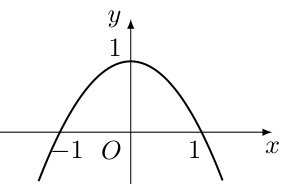
\includegraphics[width=6.0cm]{GaoKao/images/2012/hubei_science/q3_fig1.png}
\end{center}

        {\centering\begin{tabular*}{\linewidth}{@{}@{\extracolsep{\fill}}llll@{}}
          \text{A. }\( \frac{2\pi}{5} \)  &  \text{B. }\( \frac{4}{3} \)  &  \text{C. }\( \frac{3}{2} \)  &  \text{D. }\( \frac{\pi}{2} \)
        \end{tabular*}\par}

        \item 已知某几何体的三视图如图所示，则该几何体的体积为（\quad）

\begin{center}
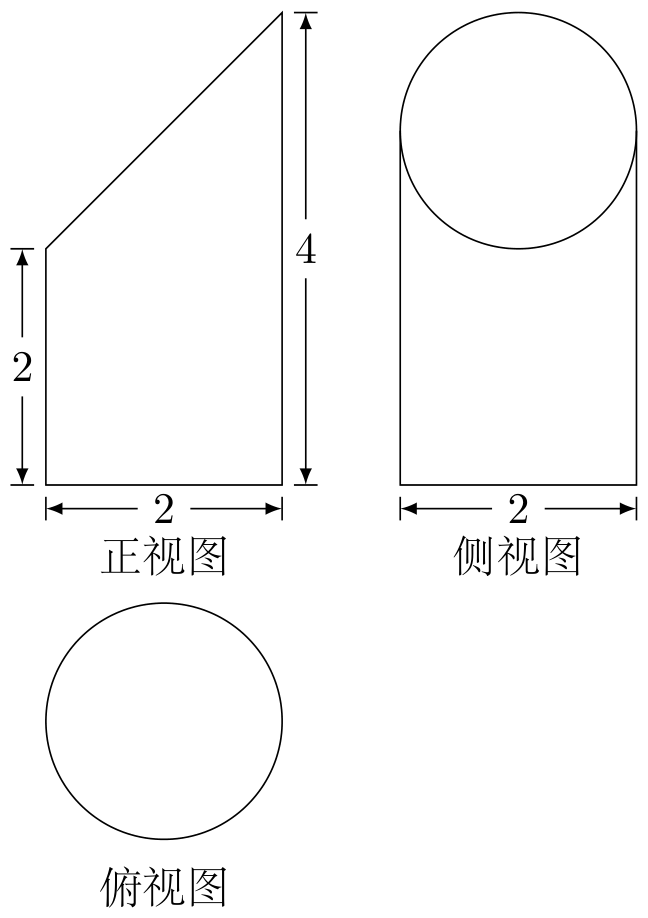
\includegraphics[width=2.7cm]{GaoKao/images/2012/hubei_science/q4_fig1.png}
\end{center}

        {\centering\begin{tabular*}{\linewidth}{@{}@{\extracolsep{\fill}}llll@{}}
          \text{A. }\(\frac{8\pi}{3}\)  &  \text{B. }\(3\pi\)  &  \text{C. }\(\frac{10\pi}{3}\)  &  \text{D. }\(6\pi\)
        \end{tabular*}\par}

        \item 设 \(a \in \mathbb{Z}\)，且 \(0 \leqslant a < 13\)，若 \(5^{12012} + a\) 能被 13 整除，则 \(a =\)（\quad）

        {\centering\begin{tabular*}{\linewidth}{@{}@{\extracolsep{\fill}}llll@{}}
          \text{A. }0  &  \text{B. }1  &  \text{C. }11  &  \text{D. }12
        \end{tabular*}\par}

        \item 设 \(a\)，\(b\)，\(c\)，\(x\)，\(y\)，\(z\) 是正数，且 \(a^2 + b^2 + c^2 = 10\)，\(x^2 + y^2 + z^2 = 40\)，\(ax + by + cz = 20\)，则 \(\frac{a + b + c}{x + y + z} =\)（\quad）

        {\centering\begin{tabular*}{\linewidth}{@{}@{\extracolsep{\fill}}llll@{}}
          \text{A. }\( \frac{1}{4} \)  &  \text{B. }\( \frac{1}{3} \)  &  \text{C. }\( \frac{1}{2} \)  &  \text{D. }\( \frac{3}{4} \)
        \end{tabular*}\par}

        \item 定义在 \((- \infty, 0) \cup (0, +\infty)\) 上的函数 \(f(x)\)，如果对于任意给定的等比数列 \(\{a_n\}\)，\(\{f(a_n)\}\) 仍是等比数列，则称 \(f(x)\) 为“保等比数列函数”. 现有定义在 \((- \infty, 0) \cup (0, +\infty)\) 上的如下函数：

\begin{enumerate}
\item \( f(x)=x^{2} \)；
\item \( f(x)=2^{x} \)；
\item \( f(x)=\sqrt{|x|} \)；
\item \( f(x)=\ln|x| \).
\end{enumerate}

则其中是“保等比数列函数”的 \(f(x)\) 的序号为（\quad）

        {\centering\begin{tabular*}{\linewidth}{@{}@{\extracolsep{\fill}}llll@{}}
          \text{A. }\ding{172}\ding{173}  &  \text{B. }\ding{174}\ding{175}  &  \text{C. }\ding{172}\ding{174}  &  \text{D. }\ding{173}\ding{175}
        \end{tabular*}\par}

        \item 如图，在圆心角为直角的扇形 \(OAB\) 中，分别以 \(OA\)，\(OB\) 为直径作两个半圆. 在扇形 \(OAB\) 内随机取一点，则此点取自阴影部分的概率是（\quad）

\begin{center}
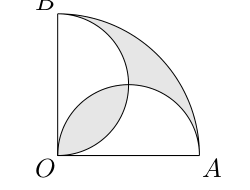
\includegraphics[width=5.0cm]{GaoKao/images/2012/hubei_science/q8_fig1.png}
\end{center}

        {\centering\begin{tabular*}{\linewidth}{@{}@{\extracolsep{\fill}}llll@{}}
          \text{A. }\(1 - \frac{2}{\pi}\)  &  \text{B. }\(\frac{1}{2} -\frac{1}{\pi}\)  &  \text{C. }\(\frac{2}{\pi}\)  &  \text{D. }\(\frac{1}{\pi}\)
        \end{tabular*}\par}

        \item 函数 \( f(x) = x\cos x^2 \) 在区间 \([0, 4]\) 上的零点个数为（\quad）

        {\centering\begin{tabular*}{\linewidth}{@{}@{\extracolsep{\fill}}llll@{}}
          \text{A. }4  &  \text{B. }5  &  \text{C. }6  &  \text{D. }7
        \end{tabular*}\par}

        \item 我国古代数学名著《九章算术》中“开立圆术”曰：置积尺数，以十六乘之，九而一，所得开立方除之，即立圆径. “开立圆术”相当于给出了已知球的体积 \(V\)，求其直径 \(d\) 的一个近似公式 \(d \approx \sqrt[3]{\frac{16}{9} V}\). 人们还用过一些类似的近似公式. 根据 \(\pi = 3.14159 \cdots\) 判断，下列近似公式中最精确的是（\quad）

        {\centering\begin{tabular*}{\linewidth}{@{}@{\extracolsep{\fill}}llll@{}}
          \text{A. }\(d \approx \sqrt[3]{\frac{16}{9} V}\)  &  \text{B. }\(d \approx \sqrt[3]{2V}\)  &  \text{C. }\(d \approx \sqrt[3]{\frac{300}{157}V}\)  &  \text{D. }\(d \approx \sqrt[3]{\frac{21}{11}V}\)
        \end{tabular*}\par}

    \end{enumerate}

\end{description}

\begin{description}

    \item[二、填空题]

    \begin{enumerate}[leftmargin=5pt]

      \addtocounter{enumi}{+10}

        \item 设 \(\triangle ABC\) 的内角 \(A\)，\(B\)，\(C\) 所对的边分别为 \(a\)，\(b\)，\(c\). 若 \((a + b - c)(a + b + c) = ab\)，则 \(C =\rule[-0.3ex]{3em}{0.4pt}\).

        \item 阅读如图所示的程序框图，运行相应的程序，

\begin{center}
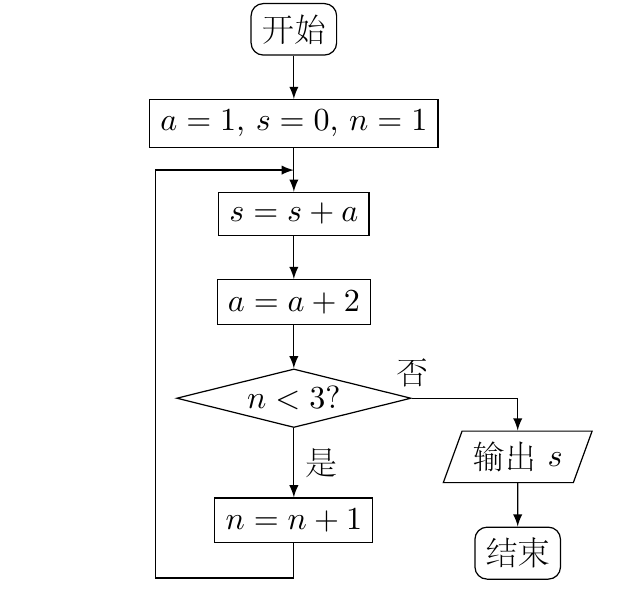
\includegraphics[width=0.42\linewidth]{GaoKao/images/2012/hubei_science/q12_fig1.png}
\end{center}

输出的结果是\rule[-0.3ex]{3em}{0.4pt}.

        \item 回文数是指从左到右读与从右到左读都一样的正整数. 如 \(22\)，\(121\)，\(3443\)，\(94249\) 等. 显然 \(2\) 位回文数有 \(9\) 个：\(11\)，\(22\)，\(33\)，…，\(99\)；\(3\) 位回文数有 \(90\) 个：\(101\)，\(111\)，\(121\)，…，\(191\)，\(202\)，…，\(999\).

\begin{enumerate}
\item 4 位回文数有\rule[-0.3ex]{3em}{0.4pt} 个；
\item \( 2n+1 \)（\( n \in \mathbb{N}^{*} \)）位回文数有\rule[-0.3ex]{3em}{0.4pt} 个.
\end{enumerate}

        \item 如图，双曲线 \(\frac{x^2}{a^2} - \frac{y^2}{b^2} = 1\)（\(a, b > 0\)）的两顶点为 \(A_1\)，\(A_2\)，虚轴两端点为 \(B_1\)，\(B_2\)，两焦点为 \(F_1\)，\(F_2\). 若以 \(A_1A_2\) 为直径的圆内切于菱形 \(F_1B_1F_2B_2\)，切点分别为 \(A\)，\(B\)，\(C\)，\(D\). 则

\begin{enumerate}
\item 双曲线的离心率 \(e =\rule[-0.3ex]{3em}{0.4pt}\)；
\item 菱形 \(F_{1}B_{1}F_{2}B_{2}\) 的面积 \(S_{1}\) 与矩形 \(ABCD\) 的面积 \(S_{2}\) 的比值 \(\frac{S_{1}}{S_{2}} =\rule[-0.3ex]{3em}{0.4pt}\).
\end{enumerate}

\begin{center}
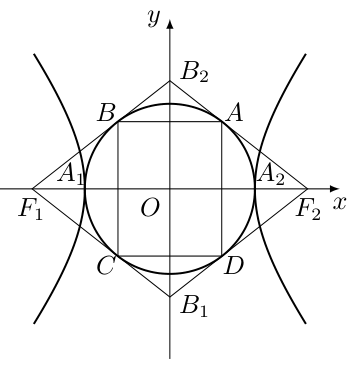
\includegraphics[width=6.2cm]{GaoKao/images/2012/hubei_science/q14_fig1.png}
\end{center}

    \end{enumerate}

\end{description}

\begin{description}

    \item[三、选考题]

    \begin{enumerate}[leftmargin=5pt]

      \addtocounter{enumi}{+14}

        \item 如图，点 \(D\) 在 \(\odot O\) 的弦 \(AB\) 上移动，\(AB = 4\). 连接 \(OD\)，过点 \(D\) 作 \(OD\) 的垂线交 \(\odot O\) 于点 \(C\)，则 \(CD\) 的最大值为\rule[-0.3ex]{3em}{0.4pt}.

\begin{center}
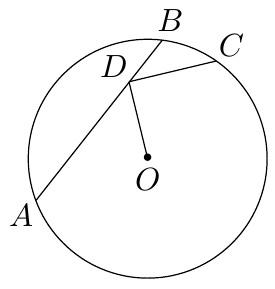
\includegraphics[width=4.5cm]{GaoKao/images/2012/hubei_science/q15_fig1.png}
\end{center}

        \item \textbf{【选修4-4：坐标系与参数方程】}

在直角坐标系 \(xOy\) 中，以原点 \(O\) 为极点，\(x\) 轴的正半轴为极轴建立极坐标系. 已知射线 \(\theta = \frac{\pi}{4}\) 与曲线 \(\begin{cases}
x = t + 1,\\
y = (t - 1)^2,
\end{cases}\) （\(t\) 为参数） 相交于 \(A\)，\(B\) 两点，则线段 \(AB\) 的中点的直角坐标为\rule[-0.3ex]{3em}{0.4pt}.

    \end{enumerate}

\end{description}

\begin{description}

    \item[四、解答题]

    \begin{enumerate}[leftmargin=5pt]

      \addtocounter{enumi}{+16}

        \item 已知向量 \( \bm{a} = (\cos \omega x - \sin \omega x, \sin \omega x) \)，\( \bm{b} = (-\cos \omega x - \sin \omega x, 2\sqrt{3} \cos \omega x) \)，设函数 \( f(x) = \bm{a} \cdot \bm{b} + \lambda \)（\(x \in \mathbb{R}\)）的图象关于直线 \(x = \pi\) 对称，其中 \(\omega\)，\(\lambda\) 为常数，且 \(\omega \in \left(\frac{1}{2}, 1\right)\).

\begin{enumerate}
\item 求函数 \( f(x) \) 的最小正周期；
\item 若 \( y = f(x) \) 的图象经过点 \( \left(\frac{\pi}{4}, 0\right)\)，求函数 \( f(x) \) 在区间 \( \left[0, \frac{3\pi}{5}\right] \) 上的取值范围.
\end{enumerate}

        \item 已知等差数列 \(\{a_{n}\}\) 前三项的和为 \(-3\)，前三项的积为 \(8\).

\begin{enumerate}
\item 求等差数列 \(\{a_{n}\}\) 的通项公式；
\item 若 \(a_{2}\)，\(a_{3}\)，\(a_{1}\) 成等比数列，求数列 \(\{|a_{n}|\}\) 的前 \(n\) 项和.
\end{enumerate}

        \item 根据以往的经验，某工程施工期间的降水量 \(X\)（单位：\(\mathrm{mm}\)）对工期的影响如下表：

\begin{center}
\begin{tabular}{c|cccc}
降水量 \(X\) & \(X < 300\) & \(300 \leqslant X < 700\) & \(700 \leqslant X < 900\) & \(X \geqslant 900\) \\
\hline
工期延误天数 \(Y\) & 0 & 2 & 6 & 10
\end{tabular}
\end{center}

历年气象资料表明，该工程施工期间降水量 \(X\) 小于 \(300\)，\(700\)，\(900\) 的概率分别为 \(0.3\)，\(0.7\)，\(0.9\). 求：

\begin{enumerate}
\item 工期延误天数 \(Y\) 的均值与方差；
\item 在降水量 \(X\) 至少是 \(300\) 的条件下，工期延误不超过 \(6\) 天的概率.
\end{enumerate}

        \item 已知函数 \( f(x) = rx - x^{r} + (1 - r) \) （\(x > 0\)），其中 \(r\) 为有理数，且 \(0 < r < 1\).

\begin{enumerate}
\item 求 \(f(x)\) 的最小值；
\item 试用（1）的结果证明如下命题：设 \(a_{1} \geqslant 0\)，\(a_{2} \geqslant 0\)，\(b_{1}\)，\(b_{2}\) 为正有理数. 若 \(b_{1} + b_{2} = 1\)，则 \(a_{1}^{b_{1}} a_{2}^{b_{2}} \leqslant a_{1} b_{1} + a_{2} b_{2}\)；
\item 请将（2）中的命题推广到一般形式，并用数学归纳法证明你所推广的命题. 注：当 \(\alpha\) 为正有理数时，有求导公式 \((x^{\alpha})^{\prime} = \alpha x^{\alpha -1}\).
\end{enumerate}

        \item 如图 1，\(\angle ACB = 45^{\circ}\)，\(BC = 3\)，过动点 \(A\) 作 \(AD \perp BC\)，垂足 \(D\) 在线段 \(BC\) 上且异于点 \(B\)，连接 \(AB\). 沿 \(AD\) 将 \(\triangle ABD\) 折起，使 \(\angle BDC = 90^{\circ}\)（如图 2 所示）.

\begin{enumerate}
\item 当 \(BD\) 的长为多少时，三棱锥 \(A - BCD\) 的体积最大；
\item 当三棱锥 \(A - BCD\) 的体积最大时，设点 \(E\)，\(M\) 分别为棱 \(BC\)，\(AC\) 的中点，试在棱 \(CD\) 上确定一点 \(N\)，使得 \(EN \perp BM\)，并求 \(EN\) 与平面 \(BMN\) 所成角的大小.
\end{enumerate}

\begin{center}
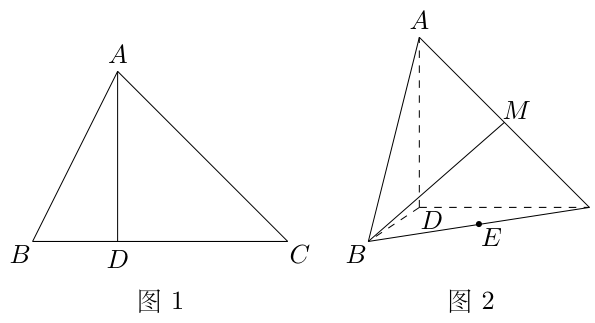
\includegraphics[width=10.0cm]{GaoKao/images/2012/hubei_science/q19_fig1.png}
\end{center}

        \item 设 \(A\) 是单位圆 \(x^{2} + y^{2} = 1\) 上的任意一点，\(l\) 是过点 \(A\) 与 \(x\) 轴垂直的直线，\(D\) 是直线 \(l\) 与 \(x\) 轴的交点，点 \(M\) 在直线 \(l\) 上，且满足 \(|DM| = m|DA|\) （\(m > 0\) 且 \(m \neq 1\)）. 当点 \(A\) 在圆上运动时，记点 \(M\) 的轨迹为曲线 \(C\).

\begin{enumerate}
\item 求曲线 \(C\) 的方程，判断曲线 \(C\) 为何种圆锥曲线. 并求其焦点坐标；
\item 过原点且斜率为 \(k\) 的直线交曲线 \(C\) 于 \(P\)，\(Q\) 两点，其中 \(P\) 在第一象限，它在 \(y\) 轴上的射影为点 \(N\)，直线 \(QN\) 交曲线 \(C\) 于另一点 \(H\). 是否存在 \(m\)，使得对任意的 \(k > 0\)，都有 \(PQ \perp PH\)？ 若存在，求 \(m\) 的值；若不存在，请说明理由.
\end{enumerate}

    \end{enumerate}

\end{description}


\subsection{2012年湖北卷（文）}\label{gk:2012年湖北卷（文）}

\begin{description}

    \item[一、选择题]

    \begin{enumerate}[leftmargin=5pt]

        \item 已知集合 \(A = \{x \mid x^2 - 3x + 2 = 0, x \in \mathbb{R}\}\)，\(B = \{x \mid 0 < x < 5, x \in \mathbb{N}\}\). 则满足条件 \(A \subseteq C \subseteq B\) 的集合 \(C\) 的个数为（\quad）

        {\centering\begin{tabular*}{\linewidth}{@{}@{\extracolsep{\fill}}llll@{}}
          \text{A. }\(1\)  &  \text{B. }\(2\)  &  \text{C. }\(3\)  &  \text{D. }\(4\)
        \end{tabular*}\par}

        \item 容量为 \(20\) 的样本数据，分组后的频数如下表：

\begin{center}
\begin{tabular}{c|cccccc}
分组 & \([10,20)\) & \([20,30)\) & \([30,40)\) & \([40,50)\) & \([50,60)\) & \([60,70)\) \\
\hline
频数 & \(2\) & \(3\) & \(4\) & \(5\) & \(4\) & \(2\)
\end{tabular}
\end{center}

则样本数据落在区间 \([10,40)\) 的频率为（\quad）

        {\centering\begin{tabular*}{\linewidth}{@{}@{\extracolsep{\fill}}llll@{}}
          \text{A. }\(0.35\)  &  \text{B. }\(0.45\)  &  \text{C. }\(0.55\)  &  \text{D. }\(0.65\)
        \end{tabular*}\par}

        \item 函数 \( f(x) = x \cos 2x \) 在区间 \([0, 2\pi]\) 上的零点的个数为（\quad）

        {\centering\begin{tabular*}{\linewidth}{@{}@{\extracolsep{\fill}}llll@{}}
          \text{A. }\(2\)  &  \text{B. }\(3\)  &  \text{C. }\(4\)  &  \text{D. }\(5\)
        \end{tabular*}\par}

        \item 命题“存在一个无理数，它的平方是有理数”的否定是（\quad）

        {\centering\begin{tabular*}{\linewidth}{@{}@{\extracolsep{\fill}}llll@{}}
          \text{A. }任意一个有理数，它的平方是有理数  &  \text{B. }任意一个无理数，它的平方不是有理数  &  \text{C. }存在一个有理数，它的平方是有理数  &  \text{D. }存在一个无理数，它的平方不是有理数
        \end{tabular*}\par}

        \item 过点 \(P(1,1)\) 的直线，将圆形区域 \(\{(x,y) | x^2 + y^2 \leqslant 4\}\) 分为两部分，使得这两部分的面积之差最大，则该直线的方程为（\quad）

        {\centering\begin{tabular*}{\linewidth}{@{}@{\extracolsep{\fill}}llll@{}}
          \text{A. }\(x + y - 2 = 0\)  &  \text{B. }\(y - 1 = 0\)  &  \text{C. }\(x - y = 0\)  &  \text{D. }\(x + 3y - 4 = 0\)
        \end{tabular*}\par}

        \item 已知定义在区间 \([0,2]\) 上的函数 \(y=f(x)\) 的图象如图所示，则 \(y=-f(2-x)\) 的图象为（\quad）

\begin{center}
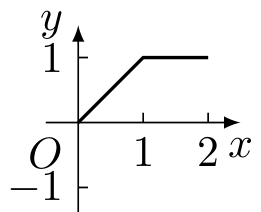
\includegraphics[width=2.6cm]{GaoKao/images/2012/hubei_liberal/q6_fig1.png}
\end{center}

        {\centering\begin{tabular*}{\linewidth}{@{}@{\extracolsep{\fill}}cccc@{}}
          \text{A. }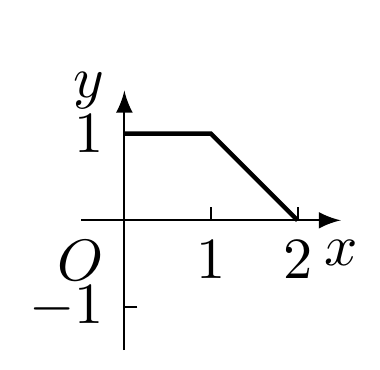
\includegraphics[width=0.15\paperwidth]{GaoKao/images/2012/hubei_liberal/q6_optA.png}  &  \text{B. }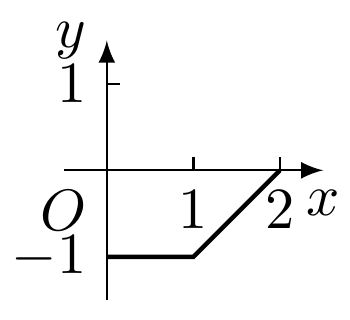
\includegraphics[width=0.15\paperwidth]{GaoKao/images/2012/hubei_liberal/q6_optB.png}  &  \text{C. }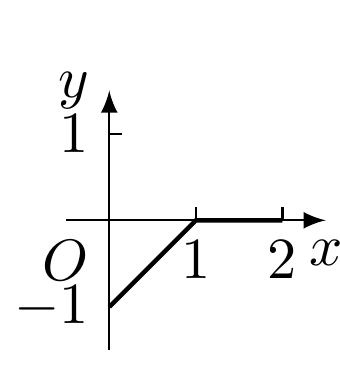
\includegraphics[width=0.15\paperwidth]{GaoKao/images/2012/hubei_liberal/q6_optC.png}  &  \text{D. }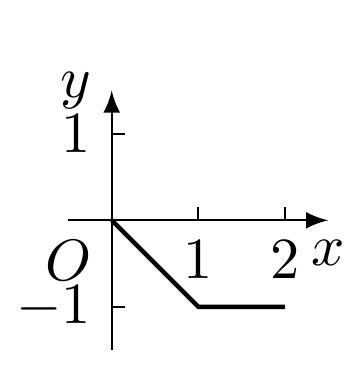
\includegraphics[width=0.15\paperwidth]{GaoKao/images/2012/hubei_liberal/q6_optD.png}
        \end{tabular*}\par}

        \item 定义在 \((- \infty, 0) \cup (0, +\infty)\) 上的函数 \(f(x)\)，如果对于任意给定的等比数列 \(\{a_{n}\}\)，\(\{f(a_{n})\}\) 仍是等比数列，则称 \(f(x)\) 为“保等比数列函数”. 现有定义在 \((- \infty, 0) \cup (0, +\infty)\) 上的如下函数：
\begin{enumerate}
\item \( f(x)=x^{2} \)；
\item \( f(x)=2^{x} \)；
\item \( f(x)=\sqrt{|x|} \)；
\item \( f(x)=\ln|x| \).
\end{enumerate}
则其中是“保等比数列函数”的 \( f(x) \) 的序号为（\quad）

        {\centering\begin{tabular*}{\linewidth}{@{}@{\extracolsep{\fill}}llll@{}}
          \text{A. }\ding{172}\ding{173}  &  \text{B. }\ding{174}\ding{175}  &  \text{C. }\ding{172}\ding{174}  &  \text{D. }\ding{173}\ding{175}
        \end{tabular*}\par}

        \item 设 \(\triangle ABC\) 的内角 \(A\)，\(B\)，\(C\) 所对的边分别为 \(a\)，\(b\)，\(c\). 若三边的长为连续的三个正整数，且 \(A > B > C\)，\(3b = 20a\cos A\)，则 \(\sin A: \sin B: \sin C\) 为（\quad）

        {\centering\begin{tabular*}{\linewidth}{@{}@{\extracolsep{\fill}}llll@{}}
          \text{A. }\(4:3:2\)  &  \text{B. }\(5:6:7\)  &  \text{C. }\(5:4:3\)  &  \text{D. }\(6:5:4\)
        \end{tabular*}\par}

        \item 设 \(a\)，\(b\)，\(c \in \mathbb{R}_{+}\)，则“\(abc = 1\)”是“\(\frac{1}{\sqrt{a}} + \frac{1}{\sqrt{b}} + \frac{1}{\sqrt{c}} \leqslant a + b + c\)”的（\quad）

        {\centering\begin{tabular*}{\linewidth}{@{}@{\extracolsep{\fill}}llll@{}}
          \text{A. }充分条件但不是必要条件  &  \text{B. }必要条件但不是充分条件  &  \text{C. }充分必要条件  &  \text{D. }既不充分也不必要的条件
        \end{tabular*}\par}

        \item 如图，在圆心角为直角的扇形 \(OAB\) 中，分别以 \(OA\)，\(OB\) 为直径作两个半圆. 在扇形 \(OAB\) 内随机取一点，则此点取自阴影部分的概率是（\quad）

\begin{center}
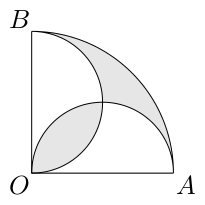
\includegraphics[width=4.0cm]{GaoKao/images/2012/hubei_liberal/q10_fig1.png}
\end{center}

        {\centering\begin{tabular*}{\linewidth}{@{}@{\extracolsep{\fill}}llll@{}}
          \text{A. }\(\frac{1}{2} -\frac{1}{\pi}\)  &  \text{B. }\(\frac{1}{\pi}\)  &  \text{C. }\(1 - \frac{2}{\pi}\)  &  \text{D. }\(\frac{2}{\pi}\)
        \end{tabular*}\par}

    \end{enumerate}

\end{description}

\begin{description}

    \item[二、填空题]

    \begin{enumerate}[leftmargin=5pt]

      \addtocounter{enumi}{+10}

        \item 一支田径运动队有男运动员 \(56\) 人，女运动员 \(42\) 人. 现用分层抽样的方法抽取若干人，若抽取的男运动员有 \(8\) 人，则抽取的女运动员有\rule[-0.3ex]{3em}{0.4pt} 人.

        \item 若 \(\frac{3 + bi}{1 - i} = a + bi\)（\(a\)，\(b\) 为实数，\(i\) 为虚数单位），则 \(a + b =\)\rule[-0.3ex]{3em}{0.4pt}.

        \item 已知向量 \(\bm{a} = (1,0)\)，\(\bm{b} = (1,1)\)，则
\begin{enumerate}
\item 与 \(2\bm{a} + \bm{b}\) 同向的单位向量的坐标表示为\rule[-0.3ex]{3em}{0.4pt}；
\item 向量 \(\bm{b} - 3\bm{a}\) 与向量 \(\bm{a}\) 夹角的余弦值为\rule[-0.3ex]{3em}{0.4pt}.
\end{enumerate}

        \item 若变量 \(x\)，\(y\) 满足约束条件 \(\begin{cases}
x - y \geqslant -1,\\
x + y \geqslant 1,\\
3x - y \leqslant 3,
\end{cases}\)
则目标函数 \(z = 2x + 3y\) 的最小值是\rule[-0.3ex]{3em}{0.4pt}.

        \item 已知某几何体的三视图如图所示，则该几何体的体积为\rule[-0.3ex]{3em}{0.4pt}.

\begin{center}
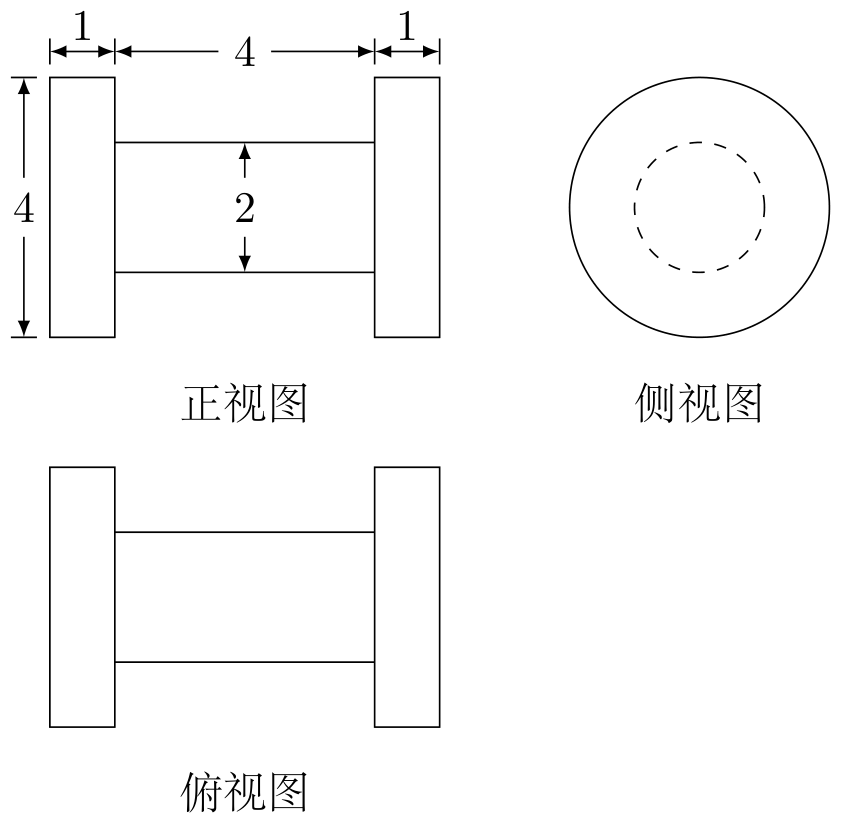
\includegraphics[width=8.2cm]{GaoKao/images/2012/hubei_liberal/q15_fig1.png}
\end{center}

        \item 阅读如图所示的程序框图，运行相应的程序，输出的结果 \(s =\)\rule[-0.3ex]{3em}{0.4pt}.

\begin{center}
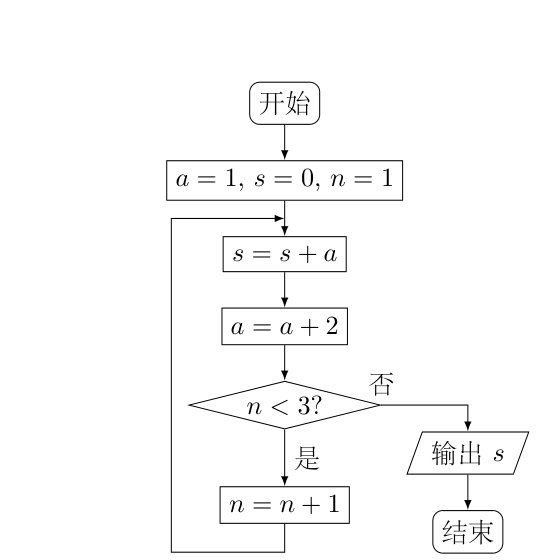
\includegraphics[width=0.42\linewidth]{GaoKao/images/2012/hubei_liberal/q16_fig1.png}
\end{center}

        \item 传说古希腊毕达哥拉斯学派的数学家经常在沙滩上画点或用小石子表示数. 他们研究过如图所示的三角形数：

将三角形数 1, 3, 6, 10, \dots 记为数列 \( \{a_{n}\} \)，记可被 5 整除的三角形数按从小到大的顺序组成一个新数列 \( \{b_{n}\} \)，可以推测：
\begin{enumerate}
\item \( b_{2012} \) 是数列 \( \{a_{n}\} \) 中的第\rule[-0.3ex]{3em}{0.4pt} 项；
\item \( b_{2k-1} =\rule[-0.3ex]{3em}{0.4pt} \)（用 \(k\) 表示）
\end{enumerate}

\begin{center}
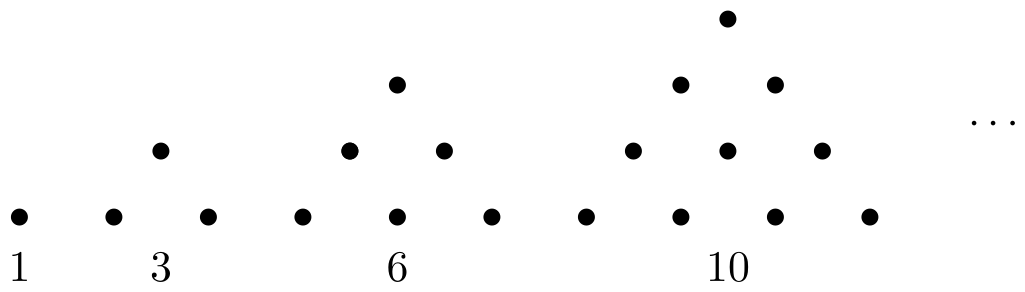
\includegraphics[width=9.9cm]{GaoKao/images/2012/hubei_liberal/q17_fig1.png}
\end{center}

    \end{enumerate}

\end{description}

\begin{description}

    \item[三、解答题]

    \begin{enumerate}[leftmargin=5pt]

      \addtocounter{enumi}{+17}

        \item 设函数 \( f(x) = \sin^2 \omega x + 2\sqrt{3}\sin \omega x \cdot \cos \omega x - \cos^2 \omega x + \lambda \)（\(x \in \mathbb{R}\)）的图象关于直线 \( x = \pi \) 对称，其中 \(\omega\)，\(\lambda\) 为常数，且 \( \omega \in \left(\frac{1}{2}, 1\right) \).
\begin{enumerate}
\item 求函数 \( f(x) \) 的最小正周期；
\item 若 \( y = f(x) \) 的图象经过点 \( \left(\frac{\pi}{4}, 0\right) \)，求函数 \( f(x) \) 的值域.
\end{enumerate}

        \item 某个实心零部件的形状是如图所示的几何体，其下部是底面均是正方形，侧面是全等的等腰梯形的四棱台 \(A_{1}B_{1}C_{1}D_{1} - ABCD\)，上部是一个底面与四棱台的上底面重合，侧面是全等的矩形的四棱柱 \(ABCD - A_{2}B_{2}C_{2}D_{2}\).
\begin{enumerate}
\item 证明：直线 \(B_{1}D_{1} \perp\) 平面 \(ACC_{2}A_{2}\)；
\item 现需要对该零部件表面进行防腐处理. 已知 \(AB = 10\)，\(A_{1}B_{1} = 20\)，\(AA_{2} = 30\)，\(AA_{1} = 13\)（单位：厘米），每平方厘米的加工处理费用为 \(0.20\text{ 元}\). 需加工处理费多少元？
\end{enumerate}

\begin{center}
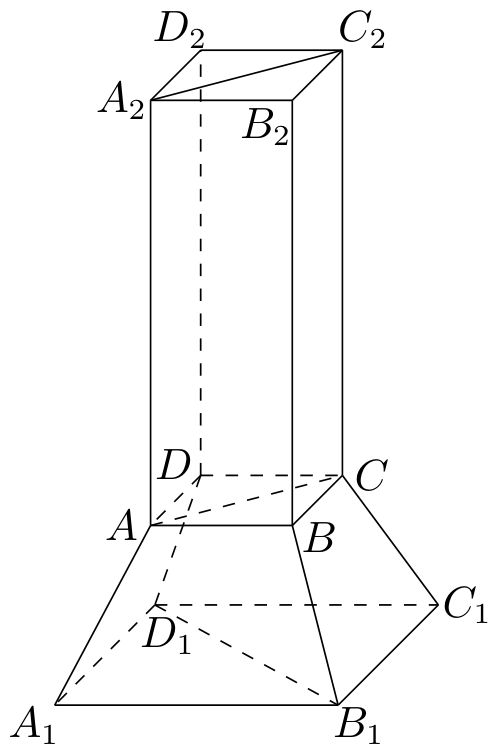
\includegraphics[width=4.9cm]{GaoKao/images/2012/hubei_liberal/q19_fig1.png}
\end{center}

        \item 已知等差数列 \(\{a_{n}\}\) 前三项的和为\(-3\)，前三项的积为8.
\begin{enumerate}
\item 求等差数列 \( \{a_{n}\} \) 的通项公式；
\item 若 \(a_{2}\)，\(a_{3}\)，\(a_{1}\) 成等比数列，求数列 \(\{|a_{n}|\}\) 的前 \(n\) 项和.
\end{enumerate}

        \item 设 \(A\) 是单位圆 \(x^{2} + y^{2} = 1\) 上的任意一点，\(l\) 是过点 \(A\) 与 \(x\) 轴垂直的直线，\(D\) 是直线 \(l\) 与 \(x\) 轴的交点，点 \(M\) 在直线 \(l\) 上，且满足 \(|DM| = m|DA|\) （\(m > 0\) 且 \(m \neq 1\)）. 当点 \(A\) 在圆上运动时，记点 \(M\) 的轨迹为曲线 \(C\).
\begin{enumerate}
\item 求曲线 \(C\) 的方程，判断曲线 \(C\) 为何种圆锥曲线. 并求其焦点坐标；
\item 过原点且斜率为 \(k\) 的直线交曲线 \(C\) 于 \(P\)，\(Q\) 两点，其中 \(P\) 在第一象限，它在 \(y\) 轴上的射影为点 \(N\)，直线 \(QN\) 交曲线 \(C\) 于另一点 \(H\). 是否存在 \(m\)，使得对任意的 \(k > 0\)，都有 \(PQ \perp PH\)？ 若存在，求 \(m\) 的值；若不存在，请说明理由.
\end{enumerate}

        \item 设函数 \( f(x) = ax^n (1 - x) + b \)（\(x > 0\)），\( n \) 为正整数，\(a\)，\(b\) 为常数. 曲线 \( y = f(x) \) 在 \( (1, f(1)) \) 处的切线方程为 \( x + y = 1 \).
\begin{enumerate}
\item 求 \(a\)，\(b\) 的值；
\item 求函数 \( f(x) \) 的最大值；
\item 证明： \( f(x) < \frac{1}{n{\mathrm{e}}} \).
\end{enumerate}

    \end{enumerate}

\end{description}


\subsection{2012年湖南卷（理）}\label{gk:2012年湖南卷（理）}

\begin{description}

    \item[一、选择题]

    \begin{enumerate}[leftmargin=5pt]

        \item 设集合 \(M=\{-1,0,1\}\)，\(N=\{x\mid x^2\leqslant x\}\)，则 \(M\cap N=\)（\quad）

        {\centering\begin{tabular*}{\linewidth}{@{}@{\extracolsep{\fill}}llll@{}}
          \text{A. }\(\{0\}\)  &  \text{B. }\(\{0,1\}\)  &  \text{C. }\(\{-1,1\}\)  &  \text{D. }\(\{-1,0,1\}\)
        \end{tabular*}\par}

        \item 命题“若 \(\alpha=\frac{\pi}{4}\)，则 \(\tan\alpha=1\)”的逆否命题是（\quad）

        {\centering\begin{tabular*}{\linewidth}{@{}@{\extracolsep{\fill}}llll@{}}
          \text{A. }若 \(\alpha\neq\frac{\pi}{4}\)，则 \(\tan\alpha\neq1\)  &  \text{B. }若 \(\alpha=\frac{\pi}{4}\)，则 \(\tan\alpha\neq1\)  &  \text{C. }若 \(\tan\alpha\neq1\)，则 \(\alpha\neq\frac{\pi}{4}\)  &  \text{D. }若 \(\tan\alpha\neq1\)，则 \(\alpha=\frac{\pi}{4}\)
        \end{tabular*}\par}

        \item 某几何体的正视图和侧视图均如下图所示，则该几何体的俯视图不可能是（\quad）

\begin{center}
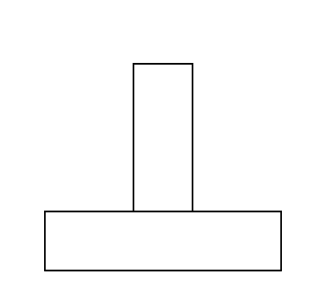
\includegraphics[width=6.0cm]{GaoKao/images/2012/hunan_science/q3_fig1.png}
\end{center}

        {\centering\begin{tabular*}{\linewidth}{@{}@{\extracolsep{\fill}}cccc@{}}
          \text{A. }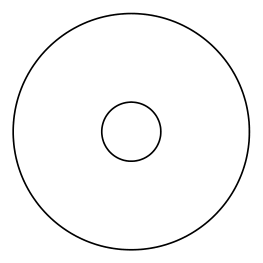
\includegraphics[width=0.15\paperwidth]{GaoKao/images/2012/hunan_science/q3_optA.png}  &  \text{B. }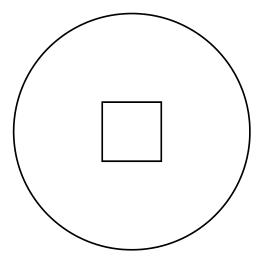
\includegraphics[width=0.15\paperwidth]{GaoKao/images/2012/hunan_science/q3_optB.png}  &  \text{C. }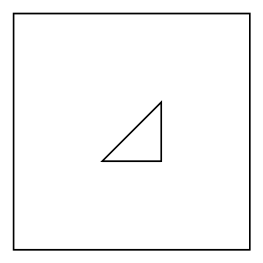
\includegraphics[width=0.15\paperwidth]{GaoKao/images/2012/hunan_science/q3_optC.png}  &  \text{D. }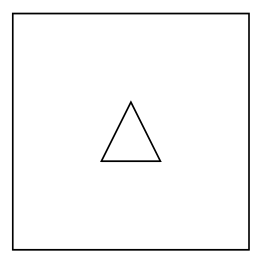
\includegraphics[width=0.15\paperwidth]{GaoKao/images/2012/hunan_science/q3_optD.png}
        \end{tabular*}\par}

        \item 设某大学的女生体重 \(y\)（单位：\(\mathrm{kg}\)）与身高 \(x\)（单位：\(\mathrm{cm}\)）具有线性相关关系，根据一组样本数据 \((x_i,y_i)\)（\(i=1\)，\(2\)，\(\cdots\)，\(n\)），用最小二乘法建立的回归方程为 \(\hat{y}=0.85x-85.71\)，则下列结论中不正确的是（\quad）

        {\centering\begin{tabular*}{\linewidth}{@{}@{\extracolsep{\fill}}llll@{}}
          \text{A. }\(y\) 与 \(x\) 具有正的线性相关关系  &  \text{B. }回归直线过样本点的中心 \((\overline{x},\overline{y})\)  &  \text{C. }若该大学某女生身高增加 \(1\,\mathrm{cm}\)，则其体重约增加 \(0.85\,\mathrm{kg}\)  &  \text{D. }若该大学某女生身高为 \(170\,\mathrm{cm}\)，则可断定其体重必为 \(58.79\,\mathrm{kg}\)
        \end{tabular*}\par}

        \item 已知双曲线 \(C:\frac{x^2}{a^2}-\frac{y^2}{b^2}=1\) 的焦距为 \(10\)，点 \(P(2,1)\) 在 \(C\) 的渐近线上，则 \(C\) 的方程为（\quad）

        {\centering\begin{tabular*}{\linewidth}{@{}@{\extracolsep{\fill}}llll@{}}
          \text{A. }\(\frac{x^2}{20}-\frac{y^2}{5}=1\)  &  \text{B. }\(\frac{x^2}{5}-\frac{y^2}{20}=1\)  &  \text{C. }\(\frac{x^2}{80}-\frac{y^2}{20}=1\)  &  \text{D. }\(\frac{x^2}{20}-\frac{y^2}{80}=1\)
        \end{tabular*}\par}

        \item 函数 \(f(x)=\sin x-\cos\left(x+\frac{\pi}{6}\right)\) 的值域为（\quad）

        {\centering\begin{tabular*}{\linewidth}{@{}@{\extracolsep{\fill}}llll@{}}
          \text{A. }\([-2,2]\)  &  \text{B. }\([-\sqrt{3},\sqrt{3}]\)  &  \text{C. }\([-1,1]\)  &  \text{D. }\(\left[-\frac{\sqrt{3}}{2},\frac{\sqrt{3}}{2}\right]\)
        \end{tabular*}\par}

        \item 在 \(\triangle ABC\) 中，\(AB=2\)，\(AC=3\)，\(\overrightarrow{AB}\cdot\overrightarrow{BC}=1\)，则 \(BC=\)（\quad）

        {\centering\begin{tabular*}{\linewidth}{@{}@{\extracolsep{\fill}}llll@{}}
          \text{A. }\(\sqrt{3}\)  &  \text{B. }\(\sqrt{7}\)  &  \text{C. }\(2\sqrt{2}\)  &  \text{D. }\(\sqrt{23}\)
        \end{tabular*}\par}

        \item 已知两条直线 \(l_1:y=m\) 和 \(l_2:y=\frac{8}{2m+1}\)（\(m>0\)），\(l_1\) 与函数 \(y=|\log_2 x|\) 的图象从左至右相交于点 \(A\)，\(B\)，\(l_2\) 与函数 \(y=|\log_2 x|\) 的图象从左至右相交于点 \(C\)，\(D\). 记线段 \(AC\) 和 \(BD\) 在 \(x\) 轴上的投影长度分别为 \(a\)，\(b\). 当 \(m\) 变化时，\(\frac{b}{a}\) 的最小值为（\quad）

        {\centering\begin{tabular*}{\linewidth}{@{}@{\extracolsep{\fill}}llll@{}}
          \text{A. }\(16\sqrt{2}\)  &  \text{B. }\(8\sqrt{2}\)  &  \text{C. }\(8\sqrt[3]{4}\)  &  \text{D. }\(4\sqrt[3]{4}\)
        \end{tabular*}\par}

    \end{enumerate}

\end{description}

\begin{description}

    \item[二、填空题]

    \begin{enumerate}[leftmargin=5pt]

      \addtocounter{enumi}{+8}

        \item 在直角坐标系 \(xOy\) 中，已知曲线 \(C_1:\begin{cases}
x=t+1,\\
y=1-2t,
\end{cases}\)（\(t\) 为参数）与曲线 \(C_2:\begin{cases}
x=a\sin\theta,\\
y=3\cos\theta,
\end{cases}\)（\(\theta\) 为参数，\(a>0\)）有一个公共点在 \(x\) 轴上，则 \(a=\)\rule[-0.3ex]{3em}{0.4pt}.

        \item 不等式 \(|2x+1|-2|x-1|>0\) 的解集为\rule[-0.3ex]{3em}{0.4pt}.

        \item 如图，过点 \(P\) 的直线与 \(\odot O\) 相交于 \(A\)，\(B\) 两点. 若 \(PA=1\)，\(AB=2\)，\(PO=3\)，则 \(\odot O\) 的半径等于\rule[-0.3ex]{3em}{0.4pt}.

\begin{center}
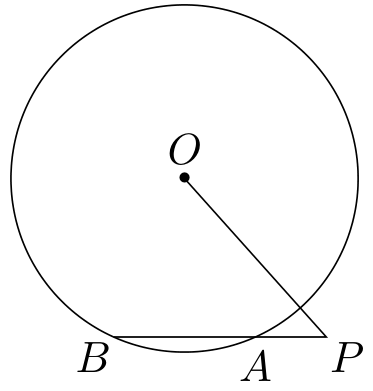
\includegraphics[width=4.5cm]{GaoKao/images/2012/hunan_science/q11_fig1.png}
\end{center}

        \item 已知复数 \(z=(3+\i)^2\)（\(\i\) 为虚数单位），则 \(|z|=\)\rule[-0.3ex]{3em}{0.4pt}.

        \item \(\left(2\sqrt{x}-\frac{1}{\sqrt{x}}\right)^6\) 的二项展开式中的常数项为\rule[-0.3ex]{3em}{0.4pt}.（用数字作答）

        \item 如果执行如图所示的程序框图，输入 \(x=-1\)，\(n=3\)，则输出的数 \(S=\)\rule[-0.3ex]{3em}{0.4pt}.

\begin{center}
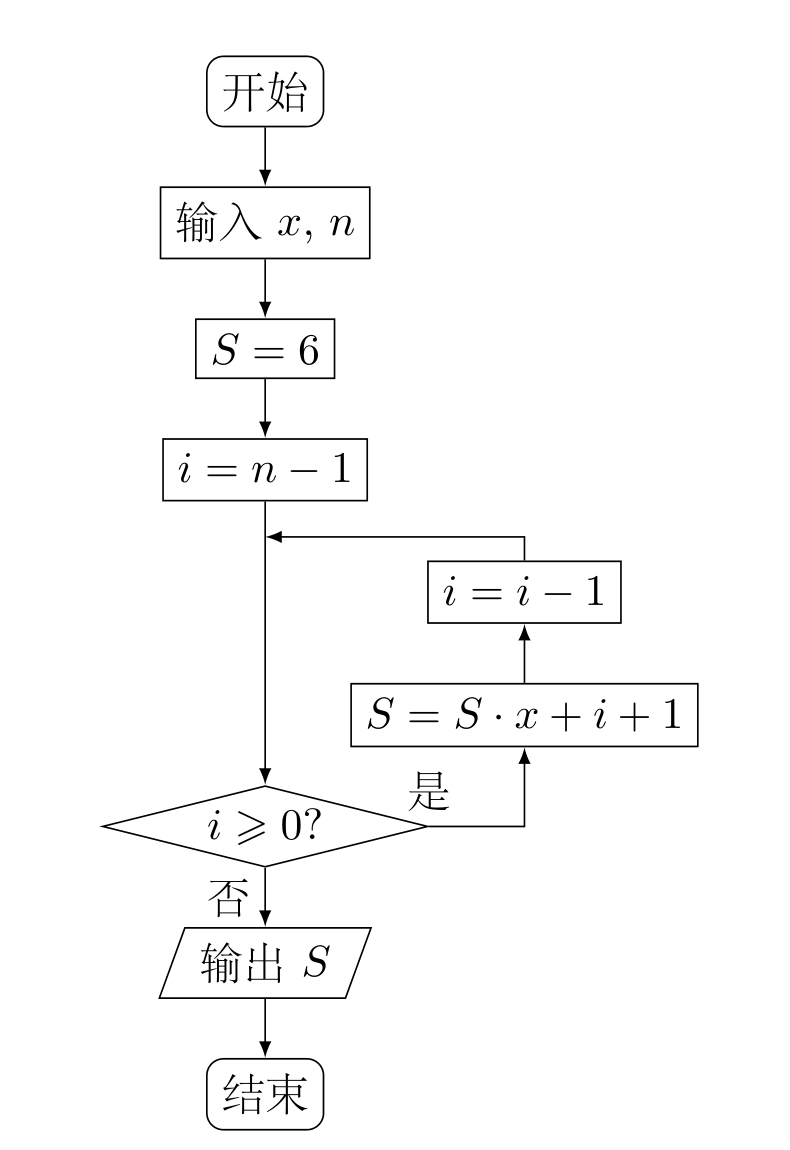
\includegraphics[width=0.56\linewidth]{GaoKao/images/2012/hunan_science/q14_fig1.png}
\end{center}

        \item 函数 \(f(x)=\sin(\omega x+\varphi)\) 的导函数 \(y=f'(x)\) 的部分图象如图所示，其中，\(P\) 为图象与 \(y\) 轴的交点，\(A\)，\(C\) 为图象与 \(x\) 轴的两个交点，\(B\) 为图象的最低点.

\begin{enumerate}
\item 若 \(\varphi=\frac{\pi}{6}\)，点 \(P\) 的坐标为 \(\left(0,\frac{3\sqrt{3}}{2}\right)\)，则 \(\omega=\)\rule[-0.3ex]{3em}{0.4pt}.
\item 若在曲线段 \(\overset{\frown}{ABC}\) 与 \(x\) 轴所围成的区域内随机取一点，则该点在 \(\triangle ABC\) 内的概率为\rule[-0.3ex]{3em}{0.4pt}.
\end{enumerate}

\begin{center}
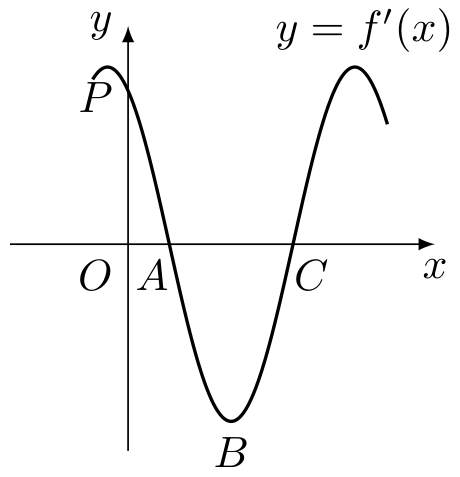
\includegraphics[width=6.0cm]{GaoKao/images/2012/hunan_science/q15_fig1.png}
\end{center}

        \item 设 \(N=2^n\)（\(n\in\mathbf{N}^*\)，\(n\geqslant2\)），将 \(N\) 个数 \(x_1\)，\(x_2\)，\(\cdots\)，\(x_N\) 依次放入编号为 \(1\)，\(2\)，\(\cdots\)，\(N\) 的 \(N\) 个位置，得到排列 \(P_0=x_1x_2\cdots x_N\). 将该排列中分别位于奇数与偶数位置的数取出，并按原顺序依次放入对应的前 \(\frac{N}{2}\) 和后 \(\frac{N}{2}\) 个位置，得到排列 \(P_1=x_1x_3\cdots x_{N-1}x_2x_4\cdots x_N\)，将此操作称为 \(C\) 变换. 将 \(P_1\) 分成两段，每段 \(\frac{N}{2}\) 个数，并对每段作 \(C\) 变换，得到 \(P_2\)；当 \(2\leqslant i\leqslant n-2\) 时，将 \(P_i\) 分成 \(2^i\) 段，每段 \(\frac{N}{2^i}\) 个数，并对每段作 \(C\) 变换，得到 \(P_{i+1}\). 例如，当 \(N=8\) 时，\(P_2=x_1x_5x_3x_7x_2x_6x_4x_8\)，此时 \(x_7\) 位于 \(P_2\) 中的第 \(4\) 个位置.

\begin{enumerate}
\item 当 \(N=16\) 时，\(x_7\) 位于 \(P_2\) 中的第\rule[-0.3ex]{3em}{0.4pt}个位置；
\item 当 \(N=2^n\)（\(n\geqslant8\)）时，\(x_{173}\) 位于 \(P_4\) 中的第\rule[-0.3ex]{3em}{0.4pt}个位置.
\end{enumerate}

    \end{enumerate}

\end{description}

\begin{description}

    \item[三、解答题]

    \begin{enumerate}[leftmargin=5pt]

      \addtocounter{enumi}{+16}

        \item 某超市为了了解顾客的购物量及结算时间等信息，安排一名员工随机收集了在该超市购物的 \(100\) 位顾客的相关数据，如下表所示.

\begin{center}
\begin{tabular}{|c|c|c|c|c|c|}
\hline
一次购物量 & 1至4件 & 5至8件 & 9至12件 & 13至16件 & 17件及以上 \\
\hline
顾客数（人） & \(x\) & 30 & 25 & \(y\) & 10 \\
\hline
结算时间（分钟/人） & 1 & 1.5 & 2 & 2.5 & 3 \\
\hline
\end{tabular}
\end{center}

已知这 \(100\) 位顾客中一次购物量超过 \(8\) 件的顾客占 \(55\%\).

\begin{enumerate}
\item 确定 \(x\)，\(y\) 的值，并求顾客一次购物的结算时间 \(X\) 的分布列与数学期望；
\item 若某顾客到达收银台时前面恰有 \(2\) 位顾客需结算，且各顾客的结算相互独立，求该顾客结算前的等候时间不超过 \(2.5\) 分钟的概率.（注：将频率视为概率）
\end{enumerate}

        \item 如图，在四棱锥 \(P-ABCD\) 中，\(PA\perp\) 平面 \(ABCD\)，\(AB=4\)，\(BC=3\)，\(AD=5\)，\(\angle DAB=\angle ABC=90^\circ\)，\(E\) 是 \(CD\) 的中点.

\begin{enumerate}
\item 证明：\(CD\perp\) 平面 \(PAE\)；
\item 若直线 \(PB\) 与平面 \(PAE\) 所成的角和 \(PB\) 与平面 \(ABCD\) 所成的角相等，求四棱锥 \(P-ABCD\) 的体积.
\end{enumerate}

\begin{center}
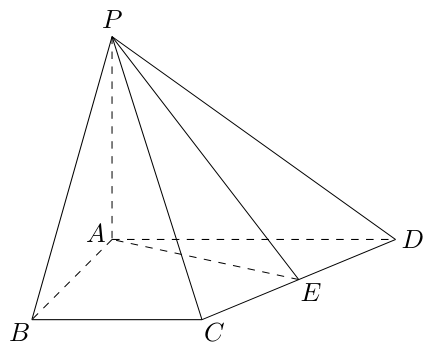
\includegraphics[width=9.0cm]{GaoKao/images/2012/hunan_science/q18_fig1.png}
\end{center}

        \item 已知数列 \(\{a_n\}\) 的各项均为正数，记 \(A(n)=a_1+a_2+\cdots+a_n\)，\(B(n)=a_2+a_3+\cdots+a_{n+1}\)，\(C(n)=a_3+a_4+\cdots+a_{n+2}\)，\(n=1\)，\(2\)，\(\cdots\).

\begin{enumerate}
\item 若 \(a_1=1\)，\(a_2=5\)，且对任意 \(n\in\mathbf{N}^*\)，三个数 \(A(n)\)，\(B(n)\)，\(C(n)\) 组成等差数列，求数列 \(\{a_n\}\) 的通项公式；
\item 证明：数列 \(\{a_n\}\) 是公比为 \(q\) 的等比数列的充分必要条件是：对任意 \(n\in\mathbf{N}^*\)，三个数 \(A(n)\)，\(B(n)\)，\(C(n)\) 组成公比为 \(q\) 的等比数列.
\end{enumerate}

        \item 某企业接到生产 \(3000\) 台某产品的 \(A\)，\(B\)，\(C\) 三种部件的订单，每台产品需要这三种部件的数量分别为 \(2\)，\(2\)，\(1\)（单位：件）. 已知每个工人每天可生产 \(A\) 部件 \(6\) 件，或 \(B\) 部件 \(3\) 件，或 \(C\) 部件 \(2\) 件. 该企业计划安排 \(200\) 名工人分成三组分别生产这三种部件，生产 \(B\) 部件的人数与生产 \(A\) 部件的人数成正比，比例系数为 \(k\)（\(k\) 为正整数）.

\begin{enumerate}
\item 设生产 \(A\) 部件的人数为 \(x\)，分别写出完成 \(A\)，\(B\)，\(C\) 三种部件生产需要的时间；
\item 假设这三种部件的生产同时开工，试确定正整数 \(k\) 的值，使完成订单任务的时间最短，并给出时间最短时具体的人数分组方案.
\end{enumerate}

        \item 在直角坐标系 \(xOy\) 中，曲线 \(C_1\) 上的点均在圆 \(C_2:(x-5)^2+y^2=9\) 外，且对 \(C_1\) 上任意一点 \(M\)，\(M\) 到直线 \(x=-2\) 的距离等于该点与圆 \(C_2\) 上点的距离的最小值.

\begin{enumerate}
\item 求曲线 \(C_1\) 的方程；
\item 设 \(P(x_0,y_0)\)（\(y_0\neq\pm3\)）为圆 \(C_2\) 外一点，过 \(P\) 作圆 \(C_2\) 的两条切线，分别与曲线 \(C_1\) 相交于点 \(A\)，\(B\) 和 \(C\)，\(D\). 证明：当 \(P\) 在直线 \(x=-4\) 上运动时，四点 \(A\)，\(B\)，\(C\)，\(D\) 的纵坐标之积为定值.
\end{enumerate}

        \item 已知函数 \(f(x)={\mathrm{e}}^{ax}-x\)，其中 \(a\neq0\).

\begin{enumerate}
\item 若对一切 \(x\in\mathbb{R}\)，\(f(x)\geqslant1\) 恒成立，求 \(a\) 的取值集合；
\item 在函数 \(f(x)\) 的图象上取定两点 \(A(x_1,f(x_1))\)，\(B(x_2,f(x_2))\)（\(x_1<x_2\)），记直线 \(AB\) 的斜率为 \(k\). 问：是否存在 \(x_0\in(x_1,x_2)\)，使 \(f'(x_0)>k\) 成立？若存在，求 \(x_0\) 的取值范围；若不存在，请说明理由.
\end{enumerate}

    \end{enumerate}

\end{description}


\subsection{2012年湖南卷（文）}\label{gk:2012年湖南卷（文）}

\begin{description}

    \item[一、选择题]

    \begin{enumerate}[leftmargin=5pt]

        \item 设集合 \(M = \{-1, 0, 1\}\)，\(N = \{x \mid x^2 = x\}\)，则 \(M \cap N =\)（\quad）

        {\centering\begin{tabular*}{\linewidth}{@{}@{\extracolsep{\fill}}llll@{}}
          \text{A. }\( \{-1,0,1\} \)  &  \text{B. }\(\{0, 1\}\)  &  \text{C. }\( \{1\} \)  &  \text{D. }\( \{0\} \)
        \end{tabular*}\par}

        \item 复数 \(z = \i(\i + 1)\)（\(\i\) 为虚数单位）的共轭复数是（\quad）

        {\centering\begin{tabular*}{\linewidth}{@{}@{\extracolsep{\fill}}llll@{}}
          \text{A. }\(-1 - \i\)  &  \text{B. }\(-1 + \i\)  &  \text{C. }\(1 - \i\)  &  \text{D. }\(1 + \i\)
        \end{tabular*}\par}

        \item 命题“若 \(\alpha = \frac{\pi}{4}\)，则 \(\tan \alpha = 1\)”的逆否命题是（\quad）

        {\centering\begin{tabular*}{\linewidth}{@{}@{\extracolsep{\fill}}llll@{}}
          \text{A. }若 \(\alpha \neq \frac{\pi}{4}\)，则 \(\tan \alpha \neq 1\)  &  \text{B. }若 \(\alpha = \frac{\pi}{4}\)，则 \(\tan \alpha \neq 1\)  &  \text{C. }若 \(\tan \alpha \neq 1\)，则 \(\alpha \neq \frac{\pi}{4}\)  &  \text{D. }若 \(\tan \alpha \neq 1\)，则 \(\alpha = \frac{\pi}{4}\)
        \end{tabular*}\par}

        \item 某几何体的正视图和侧视图均如下图所示，则该几何体的俯视图不可能是（\quad）

\begin{center}
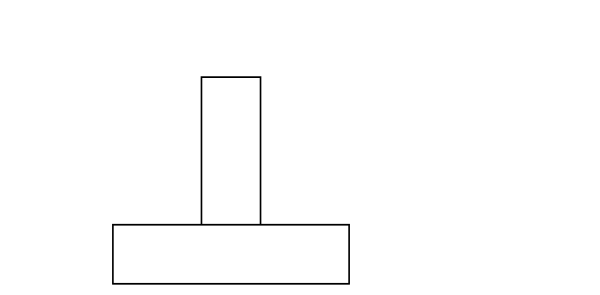
\includegraphics[width=5.0cm]{GaoKao/images/2012/hunan_liberal/q4_fig1.png}
\end{center}

        {\centering\begin{tabular*}{\linewidth}{@{}@{\extracolsep{\fill}}cccc@{}}
          \text{A. }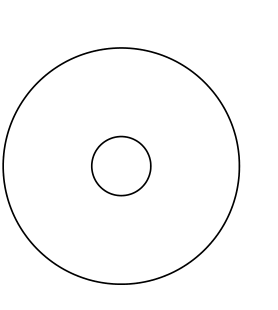
\includegraphics[width=0.15\paperwidth]{GaoKao/images/2012/hunan_liberal/q4_optA.png}  &  \text{B. }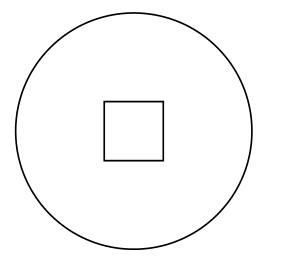
\includegraphics[width=0.15\paperwidth]{GaoKao/images/2012/hunan_liberal/q4_optB.png}  &  \text{C. }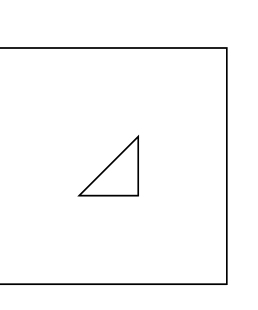
\includegraphics[width=0.15\paperwidth]{GaoKao/images/2012/hunan_liberal/q4_optC.png}  &  \text{D. }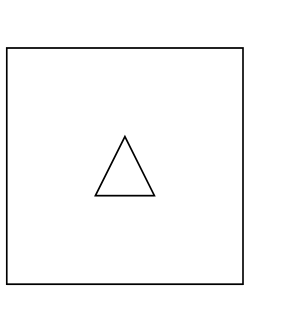
\includegraphics[width=0.15\paperwidth]{GaoKao/images/2012/hunan_liberal/q4_optD.png}
        \end{tabular*}\par}

        \item 设某大学的女生体重 \( y \) （单位： \( \mathrm{kg} \)） 与身高 \( x \) （单位： \( \mathrm{cm} \)） 具有线性相关关系，根据一组样本数据 \((x_i, y_i)\)（\(i = 1, 2, \cdots, n\)），用最小二乘法建立的回归方程为 \( \hat{y} = 0.85x - 85.71 \)，则下列结论中不正确的是（\quad）

        {\centering\begin{tabular*}{\linewidth}{@{}@{\extracolsep{\fill}}llll@{}}
          \text{A. }\(y\) 与 \(x\) 具有正的线性相关关系  &  \text{B. }回归直线过样本点的中心（\(\overline{x}\)，\(\overline{y}\)）  &  \text{C. }若该大学某女生身高增加 \(1 \mathrm{~cm}\)，则其体重约增加 \(0.85 \mathrm{~kg}\)  &  \text{D. }若该大学某女生身高为 \(170 \mathrm{~cm}\)，则可断定其体重必为 \(58.79 \mathrm{~kg}\)
        \end{tabular*}\par}

        \item 已知双曲线 \(C: \frac{x^2}{a^2} - \frac{y^2}{b^2} = 1\) 的焦距为 10，点 \(P(2,1)\) 在 \(C\) 的渐近线上，则 \(C\) 的方程为（\quad）

        {\centering\begin{tabular*}{\linewidth}{@{}@{\extracolsep{\fill}}llll@{}}
          \text{A. }\(\frac{x^2}{20} -\frac{y^2}{5} = 1\)  &  \text{B. }\(\frac{x^2}{5} -\frac{y^2}{20} = 1\)  &  \text{C. }\(\frac{x^2}{80} -\frac{y^2}{20} = 1\)  &  \text{D. }\(\frac{x^2}{20} -\frac{y^2}{80} = 1\)
        \end{tabular*}\par}

        \item 设 \(a > b > 1\)，\(c < 0\)，给出下列三个结论：
\begin{enumerate}
\item \( \frac{c}{a} > \frac{c}{b} \)；
\item \( a^{c} < b^{c} \)；
\item \( \log_{b}(a - c) > \log_{a}(b - c) \).
\end{enumerate}
其中所有正确结论的序号是（\quad）

        {\centering\begin{tabular*}{\linewidth}{@{}@{\extracolsep{\fill}}llll@{}}
          \text{A. }\ding{172}  &  \text{B. }\ding{172}\ding{173}  &  \text{C. }\ding{173}\ding{174}  &  \text{D. }\ding{172}\ding{173}\ding{174}
        \end{tabular*}\par}

        \item 在 \(\triangle ABC\) 中，\(AC = \sqrt{7}\)，\(BC = 2\)，\(B = 60^{\circ}\)，则 \(BC\) 边上的高等于（\quad）

        {\centering\begin{tabular*}{\linewidth}{@{}@{\extracolsep{\fill}}llll@{}}
          \text{A. }\(\frac{\sqrt{3}}{2}\)  &  \text{B. }\(\frac{3\sqrt{3}}{2}\)  &  \text{C. }\(\frac{\sqrt{3} + \sqrt{6}}{2}\)  &  \text{D. }\(\frac{\sqrt{3} + \sqrt{39}}{4}\)
        \end{tabular*}\par}

        \item 设定义在 \(\mathbb{R}\) 上的函数 \(f(x)\) 是最小正周期为 \(2\pi\) 的偶函数，\(f'(x)\) 是 \(f(x)\) 的导函数. 当 \(x \in [0, \pi]\) 时，\(0 < f(x) < 1\)；当 \(x \in (0, \pi)\) 且 \(x \neq \frac{\pi}{2}\) 时，\(\left(x - \frac{\pi}{2}\right)f'(x) > 0\)，则函数 \(y = f(x) - \sin x\) 在 \([-2\pi, 2\pi]\) 上的零点个数为（\quad）

        {\centering\begin{tabular*}{\linewidth}{@{}@{\extracolsep{\fill}}llll@{}}
          \text{A. }2  &  \text{B. }4  &  \text{C. }5  &  \text{D. }8
        \end{tabular*}\par}

    \end{enumerate}

\end{description}

\begin{description}

    \item[二、填空题]

    \begin{enumerate}[leftmargin=5pt]

      \addtocounter{enumi}{+9}

        \item 在极坐标系中，曲线 \(C: \rho (\sqrt{2} \cos \theta + \sin \theta) = 1\) 与曲线 \(C_{2}: \rho = a\) （\(a > 0\)） 的一个交点在极轴上，则 \(a =\rule[-0.3ex]{3em}{0.4pt}\).

        \item 某制药企业为了对某种药用液体进行生物测定，需要优选培养温度，试验范围为 \(29^{\circ} \mathrm{C} \sim 63^{\circ} \mathrm{C}\)，精确度要求 \(\pm 1^{\circ} \mathrm{C}\). 用分数法进行优选时，能保证找到最佳培养温度需要的最少试验次数为\rule[-0.3ex]{3em}{0.4pt}.

        \item 不等式 \(x^{2} - 5x + 6 \leqslant 0\) 的解集为\rule[-0.3ex]{3em}{0.4pt}.

        \item 如图是某学校一名篮球运动员在五场比赛中所得分数的茎叶图，则该运动员在这五场比赛中得分的方差为\rule[-0.3ex]{3em}{0.4pt}.
\begin{center}
\begin{tabular}{c|ccc}
\(0\) & \(8\) & \(9\) & \(3\) \\
\(1\) & \(0\) & \(3\) & \(5\)
\end{tabular}
\end{center}
（注：方差 \( s^{2}=\frac{1}{n}\left[(x_{1}-\overline{x})^{2}+(x_{2}-\overline{x})^{2}+\cdots+(x_{n}-\overline{x})^{2}\right] \)，其中 \( \overline{x} \) 为 \(x_{1}\)，\(x_{2}\)，\(\cdots\)，\(x_{n}\) 的平均数）

        \item 如果执行如图所示的程序框图，输入 \(x = 4.5\)，则输出的数 \(i =\rule[-0.3ex]{3em}{0.4pt}\).
\begin{center}
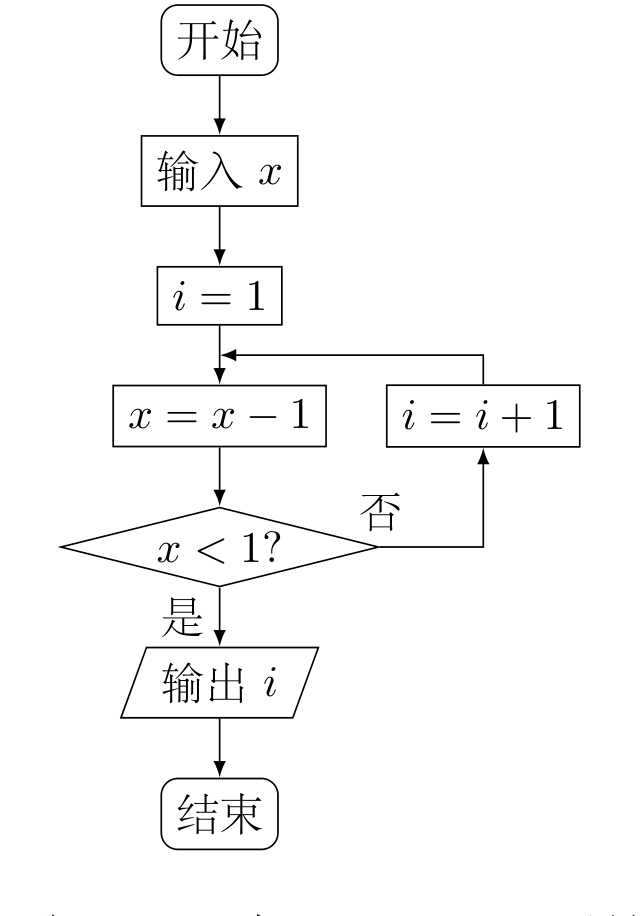
\includegraphics[width=0.65\linewidth]{GaoKao/images/2012/hunan_liberal/q14_fig1.png}
\end{center}

        \item 如图，在平行四边形 \(ABCD\) 中，\(AP \perp BD\)，垂足为 \(P\)，且 \(AP = 3\)，则 \(\overrightarrow{AP} \cdot \overrightarrow{AC} =\)\rule[-0.3ex]{3em}{0.4pt}.
\begin{center}
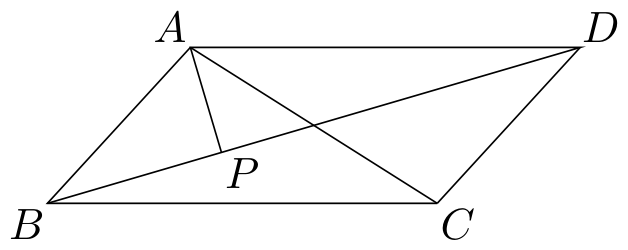
\includegraphics[width=7.8cm]{GaoKao/images/2012/hunan_liberal/q15_fig1.png}
\end{center}

        \item 对于 \(n \in \mathbf{N}^*\)，将 \(n\) 表示为 \(n = a_k \times 2^k + a_{k-1} \times 2^{k-1} + \cdots + a_1 \times 2^1 + a_0 \times 2^0\)，当 \(i = k\) 时，\(a_i = 1\)，当 \(0 \leqslant i \leqslant k - 1\) 时，\(a_i\) 为 0 或 1. 定义 \(b_n\) 如下：在 \(n\) 的上述表示中，当 \(a_0\)，\(a_1\)，\(a_2\)，\(\cdots\)，\(a_k\) 中等于 1 的个数为奇数时，\(b_n = 1\)；否则 \(b_n = 0\).
\begin{enumerate}
\item \( b_{2}+b_{4}+b_{6}+b_{8}=\rule[-0.3ex]{3em}{0.4pt}\)；
\item 记 \(c_{m}\) 为数列 \(\{b_{n}\}\) 中第 \(m\) 个为 0 的项与第 \(m + 1\) 个为 0 的项之间的项数，则 \(c_{m}\) 的最大值是\rule[-0.3ex]{3em}{0.4pt}.
\end{enumerate}

    \end{enumerate}

\end{description}

\begin{description}

    \item[三、解答题]

    \begin{enumerate}[leftmargin=5pt]

      \addtocounter{enumi}{+16}

        \item 某超市为了解顾客的购物量及结算时间等信息，安排一名员工随机收集了在该超市购物的 100 位顾客的相关数据，如下表所示.

\begin{center}
\begin{tabular}{c|ccccc}
一次购物量 & \(1\text{\ 至\ }4\)件 & \(5\text{\ 至\ }8\)件 & \(9\text{\ 至\ }12\)件 & \(13\text{\ 至\ }16\)件 & \(17\)件及以上 \\
\hline
顾客数（人） & \(x\) & 30 & 25 & \(y\) & 10 \\
\hline
结算时间（分钟/人） & 1 & 1.5 & 2 & 2.5 & 3
\end{tabular}
\end{center}

已知这 100 位顾客中一次购物量超过 8 件的顾客占 55\%.
\begin{enumerate}
\item 确定 \(x\)，\(y\) 的值，并估计顾客一次购物的结算时间的平均值；
\item 求一位顾客一次购物的结算时间不超过 2 分钟的概率. （将频率视为概率）
\end{enumerate}

        \item 已知函数 \( f(x) = A \sin (\omega x + \varphi) \) （\(x \in \mathbb{R}\)，\(\omega > 0\)，\(0 < \varphi < \tfrac{\pi}{2}\)）的部分图象如图所示.

\begin{enumerate}
\item 求函数 \( f(x) \) 的解析式；
\item 求函数 \( g(x)=f\left(x-\frac{\pi}{12}\right)-f\left(x+\frac{\pi}{12}\right) \) 的单调递增区间.
\end{enumerate}
\begin{center}
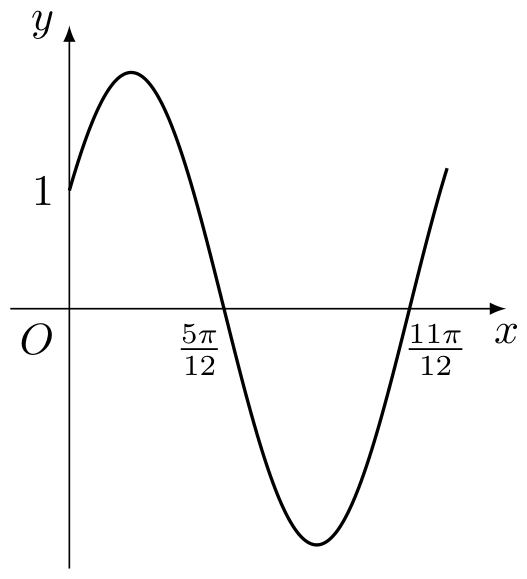
\includegraphics[width=7.8cm]{GaoKao/images/2012/hunan_liberal/q18_fig1.png}
\end{center}

        \item 如图，在四棱锥 \(P - ABCD\) 中，\(PA \perp\) 平面 \(ABCD\)，底面 \(ABCD\) 是等腰梯形，\(AD // BC\)，\(AC \perp BD\).

\begin{enumerate}
\item 证明： \(BD \perp PC\)；
\item 若 \(AD=4\)，\(BC=2\)，直线 \(PD\) 与平面 \(PAC\) 所成的角为 \(30^{\circ}\)，求四棱锥 \(P-ABCD\) 的体积.
\end{enumerate}
\begin{center}
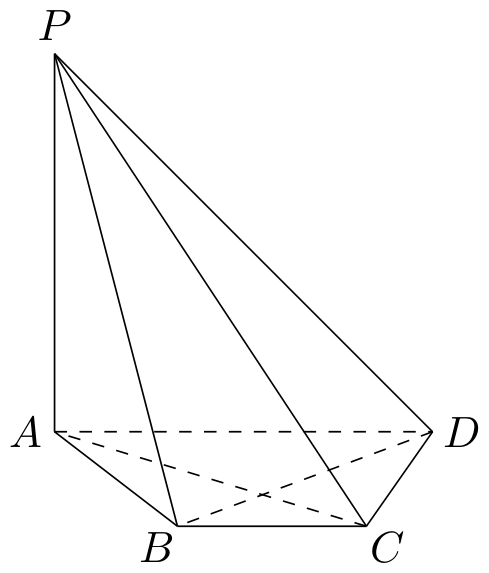
\includegraphics[width=6.1cm]{GaoKao/images/2012/hunan_liberal/q19_fig1.png}
\end{center}

        \item 某公司一下属企业从事某种高科技产品的生产. 该企业第一年年初有资金2000万元，将其投入生产，到当年年底资金增长了 \(50\%\)，预计以后每年资金年增长率与第一年的相同. 公司要求企业从第一年开始，每年年底上缴资金 \(d\) 万元，并将剩余资金全部投入下一年生产. 设第 \(n\) 年年底企业上缴资金后的剩余资金为 \(a_{n}\) 万元.
\begin{enumerate}
\item 用 \(d\) 表示 \(a_{1}\)，\(a_{2}\)，并写出 \( \{a_{n+1}\} \) 与 \( a_{n} \) 的关系式；
\item 若公司希望经过 \(m\) 年（\(m \geqslant 3\)）使企业的剩余资金为 \(4000\) 万元，试确定企业每年上缴资金 \(d\) 的值（用 \(m\) 表示）.
\end{enumerate}

        \item 在直角坐标系 \(xOy\) 中，已知中心在原点，离心率为 \(\frac{1}{2}\) 的椭圆 \(E\) 的一个焦点为圆 \(C: x^2 + y^2 - 4x + 2 = 0\) 的圆心.
\begin{enumerate}
\item 求椭圆 \(E\) 的方程；
\item 设 \(P\) 是椭圆 \(E\) 上一点，过 \(P\) 作两条斜率之积为 \(\frac{1}{2}\) 的直线 \(l_{1}\)，\(l_{2}\)，当直线 \(l_{1}\)，\(l_{2}\) 都与圆 \(C\) 相切时，求 \(P\) 的坐标.
\end{enumerate}

        \item 已知函数 \( f(x) = {\mathrm{e}}^{x} - ax \)，其中 \( a > 0 \).
\begin{enumerate}
\item 若对一切 \(x \in \mathbb{R}\)，\(f(x) \geqslant 1\) 恒成立，求 \(a\) 的取值集合；
\item 在函数 \(f(x)\) 的图象上取定两点 \(A(x_{1}, f(x_{1}))\)，\(B(x_{2}, f(x_{2}))\)（\(x_{1} < x_{2}\)），记直线 \(AB\) 的斜率为 \(k\)，证明：存在 \(x_{0} \in (x_{1}, x_{2})\)，使 \(f'(x_{0}) = k\) 成立.
\end{enumerate}

    \end{enumerate}

\end{description}


\subsection{2012年江苏卷}\label{gk:2012年江苏卷}

\begin{description}

    \item[一、填空题]

    \begin{enumerate}[leftmargin=5pt]

        \item 已知集合 \(A = \{1, 2, 4\}\)，\(B = \{2, 4, 6\}\)，则 \(A \cup B =\rule[-0.3ex]{3em}{0.4pt}.\)

        \item 某学校高一、高二、高三年级的学生人数之比是 \(3:3:4\). 现用分层抽样的方法从该校高中三个年级的学生中抽取容量为 \(50\) 的样本. 则应从高二年级抽取\rule[-0.3ex]{3em}{0.4pt} 名学生.

        \item 设 \(a,b \in \mathbb{R}\)，\(a + b\i = \frac{11 - 7\i}{1 - 2\i}\)（\(\i\) 为虚数单位），则 \(a + b\) 的值为\rule[-0.3ex]{3em}{0.4pt}.

        \item 如图是一个算法流程图，则输出的 \(k\) 的值是\rule[-0.3ex]{3em}{0.4pt}.

\begin{center}
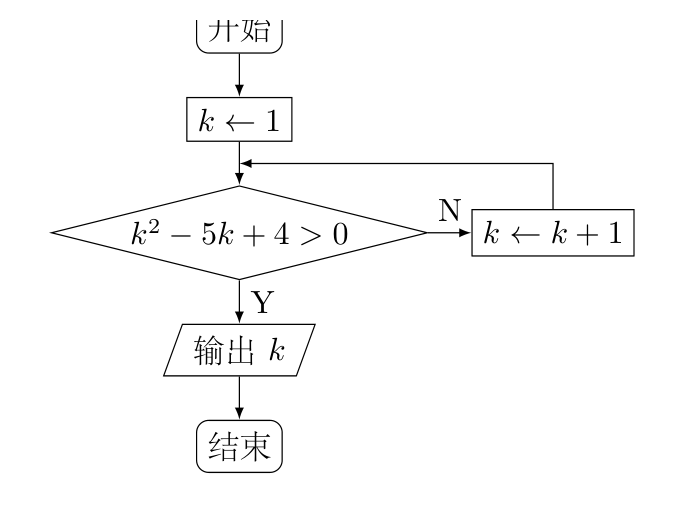
\includegraphics[width=0.46\linewidth]{GaoKao/images/2012/jiangsu/q4_fig1.png}
\end{center}

        \item 函数 \(f(x)=\sqrt{1-2\log_{6}x}\) 的定义域为\rule[-0.3ex]{3em}{0.4pt}.

        \item 现有 \(10\) 个数，它们能构成一个以 \(1\) 为首项，\(-3\) 为公比的等比数列，若从这 \(10\) 个数中随机抽取一个数，则它小于 \(8\) 的概率是\rule[-0.3ex]{3em}{0.4pt}.

        \item 如图，在长方体 \(ABCD-A_{1}B_{1}C_{1}D_{1}\) 中，\(AB = AD = 3 \mathrm{~cm}\)，\(AA_{1} = 2 \mathrm{~cm}\)，则四棱锥 \(A-BB_{1}D_{1}D\) 的体积为\rule[-0.3ex]{3em}{0.4pt} \(\mathrm{cm}^{3}\).

\begin{center}
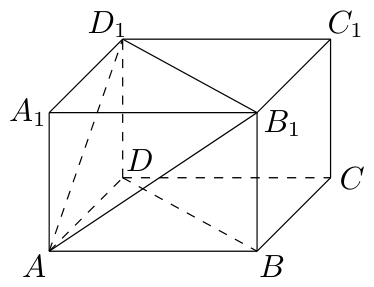
\includegraphics[width=5.3cm]{GaoKao/images/2012/jiangsu/q7_fig1.png}
\end{center}

        \item 在平面直角坐标系 \(xOy\) 中，若双曲线 \(\frac{x^2}{m} - \frac{y^2}{m^2 + 4} = 1\) 的离心率为 \(\sqrt{5}\)，则 \(m\) 的值为\rule[-0.3ex]{3em}{0.4pt}.

        \item 如图，在矩形 \(ABCD\) 中，\(AB = \sqrt{2}\)，\(BC = 2\)，点 \(E\) 为 \(BC\) 的中点，点 \(F\) 在边 \(CD\) 上，若 \(\overrightarrow{AB} \cdot \overrightarrow{AF} = \sqrt{2}\)，则 \(\overrightarrow{AE} \cdot \overrightarrow{BF}\) 的值是\rule[-0.3ex]{3em}{0.4pt}.

\begin{center}
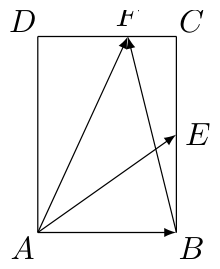
\includegraphics[width=5.1cm]{GaoKao/images/2012/jiangsu/q9_fig1.png}
\end{center}

        \item 设 \(f(x)\) 是定义在 \(\mathbb{R}\) 上且周期为 \(2\) 的函数，且在区间 \([-1,1]\) 上， \(f(x)=\begin{cases}
ax+1, & -1 \leqslant x < 0,\\
\frac{bx+2}{x+1}, & 0 \leqslant x \leqslant 1,
\end{cases}\)
其中 \(a,b \in \mathbb{R}\). 若 \(f\left(\frac{1}{2}\right)=f\left(\frac{3}{2}\right)\)，则 \(a + 3b\) 的值为\rule[-0.3ex]{3em}{0.4pt}.

        \item 设 \(\alpha\) 为锐角，若 \(\cos\left(\alpha + \frac{\pi}{6}\right)=\frac{4}{5}\)，则 \(\sin\left(2\alpha + \frac{\pi}{12}\right)\) 的值为\rule[-0.3ex]{3em}{0.4pt}.

        \item 在平面直角坐标系 \(xOy\) 中，圆 \(C\) 的方程为 \(x^2 + y^2 - 8x + 15 = 0\)，若直线 \(y = kx - 2\) 上至少存在一点，使得以该点为圆心，\(1\) 为半径的圆与圆 \(C\) 有公共点，则 \(k\) 的最大值是\rule[-0.3ex]{3em}{0.4pt}.

        \item 已知函数 \(f(x)=x^2+ax+b\)（\(a\)，\(b\in\mathbb{R}\)）的值域为 \([0,+\infty)\)，若关于 \(x\) 的不等式 \(f(x)<c\) 的解集为 \((m,m+6)\)，则实数 \(c\) 的值为\rule[-0.3ex]{3em}{0.4pt}.

        \item 已知正数 \(a\)，\(b\)，\(c\) 满足 \(5c-3a \leqslant b \leqslant 4c-a\)，\(c \ln b \geqslant a + c \ln c\)，则 \(\frac{b}{a}\) 的取值范围是\rule[-0.3ex]{3em}{0.4pt}.

    \end{enumerate}

\end{description}

\begin{description}

    \item[二、解答题]

    \begin{enumerate}[leftmargin=5pt]

      \addtocounter{enumi}{+14}

        \item 在 \(\triangle ABC\) 中，已知 \(\overrightarrow{AB} \cdot \overrightarrow{AC} = 3\overrightarrow{BA} \cdot \overrightarrow{BC}\).

\begin{enumerate}
\item 求证：\(\tan B = 3\tan A\).
\item 若 \(\cos C = \frac{\sqrt{5}}{5}\)，求 \(A\) 的值.
\end{enumerate}

        \item 如图，在直三棱柱 \(ABC-A_{1}B_{1}C_{1}\) 中，\(A_{1}B_{1}=A_{1}C_{1}\)，\(D\)，\(E\) 分别是棱 \(BC\)，\(CC_{1}\) 上的点（点 \(D\) 不同于点 \(C\)），且 \(AD \perp DE\)，\(F\) 为 \(B_{1}C_{1}\) 的中点. 求证：

\begin{enumerate}
\item 平面 \(ADE \perp\) 平面 \(BCC_{1}B_{1}\)；
\item 直线 \(A_{1}F \parallel\) 平面 \(ADE\).
\end{enumerate}
\begin{center}
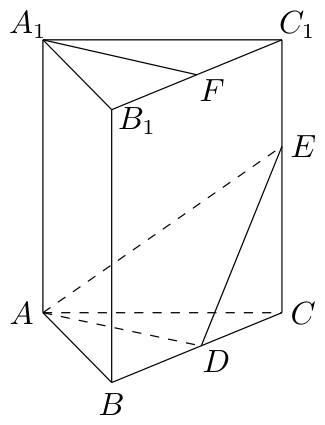
\includegraphics[width=4.4cm]{GaoKao/images/2012/jiangsu/q16_fig1.png}
\end{center}

        \item 如图，建立平面直角坐标系 \(xOy\)，\(x\) 轴在地平面上，\(y\) 轴垂直于地平面，单位长度为 \(1\) 千米，某炮位于坐标原点. 已知炮弹发射后的轨迹在方程 \(y = kx - \frac{1}{20}(1+k^2)x^2\)（\(k>0\)）表示的曲线上，其中 \(k\) 与发射方向有关. 炮的射程是指炮弹落地点的横坐标.

\begin{enumerate}
\item 求炮的最大射程；
\item 设在第一象限有一飞行物（忽略其大小），其飞行高度为 \(3.2\) 千米，试问它的横坐标 \(a\) 不超过多少时，炮弹可以击中它？请说明理由.
\end{enumerate}
\begin{center}
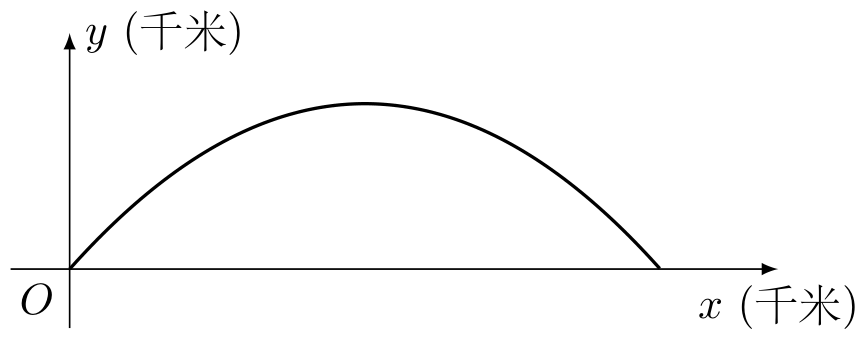
\includegraphics[width=11.0cm]{GaoKao/images/2012/jiangsu/q17_fig1.png}
\end{center}

        \item 若函数 \(y=f(x)\) 在 \(x=x_{0}\) 处取得极大值或极小值，则称 \(x_{0}\) 为函数 \(y=f(x)\) 的极值点. 已知 \(a\)，\(b\) 是实数，且 \(1\) 和 \(-1\) 是函数 \(f(x)=x^3+ax^2+bx\) 的两个极值点.

\begin{enumerate}
\item 求 \(a\) 和 \(b\) 的值；
\item 设函数 \(g(x)\) 的导函数 \(g'(x)=f(x)+2\)，求 \(g(x)\) 的极值点；
\item 设 \(h(x)=f(f(x))-c\)，其中 \(c\in[-2,2]\)，求函数 \(y=h(x)\) 的零点个数.
\end{enumerate}

        \item 如图，在平面直角坐标系 \(xOy\) 中，椭圆 \(\frac{x^2}{a^2} + \frac{y^2}{b^2} = 1\)（\(a>b>0\)）的左、右焦点分别为 \(F_{1}(-c,0)\)，\(F_{2}(c,0)\). 已知点 \((1,e)\) 和 \(\left(e,\frac{\sqrt{3}}{2}\right)\) 都在椭圆上，其中 \(e\) 为椭圆的离心率.

\begin{enumerate}
\item 求椭圆的方程；
\item 设 \(A\)，\(B\) 是椭圆上位于 \(x\) 轴上方的两点，且直线 \(AF_{1}\) 与直线 \(BF_{2}\) 平行，\(AF_{2}\) 与 \(BF_{1}\) 交于点 \(P\).
\begin{enumerate}
\item 若 \(AF_{1}-BF_{2}=\frac{\sqrt{6}}{2}\)，求直线 \(AF_{1}\) 的斜率；
\item 求证：\(PF_{1}+PF_{2}\) 是定值.
\end{enumerate}
\end{enumerate}

\begin{center}
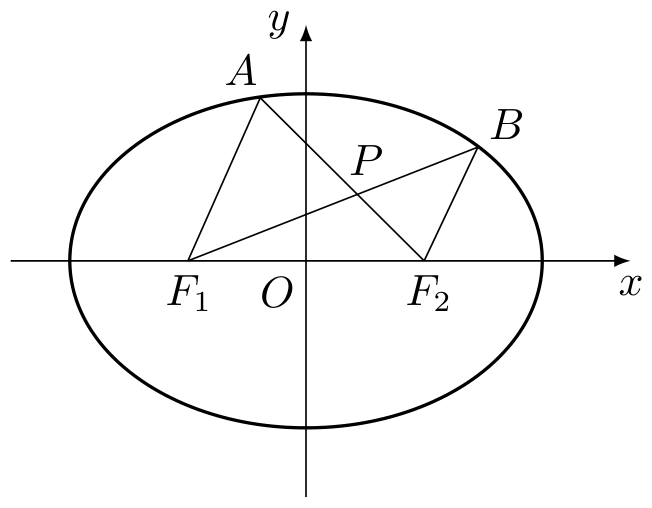
\includegraphics[width=7.8cm]{GaoKao/images/2012/jiangsu/q19_fig1.png}
\end{center}

        \item 已知各项均为正数的两个数列 \(\{a_n\}\) 和 \(\{b_n\}\) 满足：\(a_{n+1} = \frac{a_n + b_n}{\sqrt{a_n^2 + b_n^2}}\)，\(n \in \mathbf{N}^*\).

\begin{enumerate}
\item 设 \(b_{n+1} = 1 + \frac{b_n}{a_n}\)，\(n \in \mathbf{N}^*\)，求证：数列 \(\left\{\left(\frac{b_n}{a_n}\right)^2\right\}\) 是等差数列；
\item 设 \(b_{n+1} = \sqrt{2} \cdot \frac{b_n}{a_n}\)，\(n \in \mathbf{N}^*\)，且 \(\{a_n\}\) 是等比数列，求 \(a_1\) 和 \(b_1\) 的值.
\end{enumerate}

    \end{enumerate}

\end{description}

\begin{description}

    \item[三、附加题]

    \begin{enumerate}[leftmargin=5pt]

      \addtocounter{enumi}{+20}

        \item [A]
如图，\(AB\) 是圆 \(O\) 的直径，\(D\)，\(E\) 为圆 \(O\) 上位于 \(AB\) 异侧的两点，连接 \(BD\) 并延长至点 \(C\)，使 \(BD=DC\)，连接 \(AC\)，\(AE\)，\(DE\). 求证：\(\angle E=\angle C\).

\begin{center}
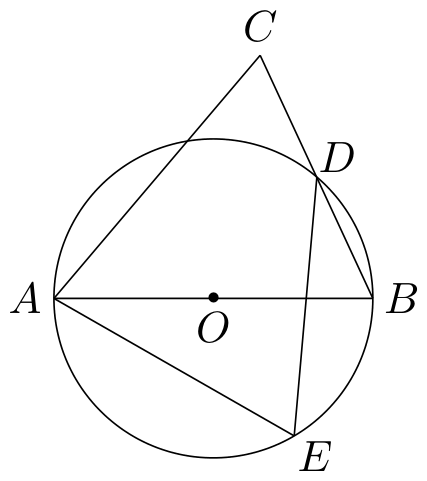
\includegraphics[width=5.0cm]{GaoKao/images/2012/jiangsu/q21_fig1.png}
\end{center}

        \item [B]
已知矩阵 \(A\) 的逆矩阵 \(A^{-1}=\begin{bmatrix}-\frac{1}{4}&\frac{3}{4}\\ \frac{1}{2}&-\frac{1}{2}\end{bmatrix}\)，求矩阵 \(A\) 的特征值.

        \item [C]
在极坐标系中，已知圆 \(C\) 经过点 \(P\left(\sqrt{2},\frac{\pi}{4}\right)\)，圆心为直线 \(\rho\sin\left(\theta-\frac{\pi}{3}\right)=-\frac{\sqrt{3}}{2}\) 与极轴的交点，求圆 \(C\) 的极坐标方程.

        \item [D]
已知实数 \(x\)，\(y\) 满足：\(|x+y|<\frac{1}{3}\)，\(|2x-y|<\frac{1}{6}\)，求证：\(|y|<\frac{5}{18}\).

        \item 设 \(\xi\) 为随机变量，从棱长为 \(1\) 的正方体的 \(12\) 条棱中任取两条，当两条棱相交时，\(\xi=0\)；当两条棱平行时，\(\xi\) 的值为两条棱之间的距离；当两条棱异面时，\(\xi=1\).

\begin{enumerate}
\item 求概率 \(P(\xi=0)\)；
\item 求 \(\xi\) 的分布列，并求其数学期望 \(E(\xi)\).
\end{enumerate}

        \item 设集合 \(P_n = \{1,2,\cdots,n\}\)，\(n \in \mathbf{N}^*\). 记 \(f(n)\) 为同时满足下列条件的集合 \(A\) 的个数：
\begin{enumerate}
\item \(A \subseteq P_n\)；
\item 若 \(x \in A\)，则 \(2x \notin A\)；
\item 若 \(x \in C_{P_n}A\)，则 \(2x \notin C_{P_n}A\).
\end{enumerate}

\begin{enumerate}
\item 求 \(f(4)\)；
\item 求 \(f(n)\) 的解析式（用 \(n\) 表示）.
\end{enumerate}

    \end{enumerate}

\end{description}


\subsection{2012年江西卷（理）}\label{gk:2012年江西卷（理）}

\begin{description}

    \item[一、选择题]

    \begin{enumerate}[leftmargin=5pt]

        \item 若集合 \(A = \{-1, 1\}\)，\(B = \{0, 2\}\)，则集合 \(\{z \mid z = x + y, x \in A, y \in B\}\) 中的元素个数为（\quad）

        {\centering\begin{tabular*}{\linewidth}{@{}@{\extracolsep{\fill}}llll@{}}
          \text{A. }5  &  \text{B. }4  &  \text{C. }3  &  \text{D. }2
        \end{tabular*}\par}

        \item 下列函数中，与函数 \( y = \frac{1}{\sqrt[3]{x}} \) 定义域相同的函数为（\quad）

        {\centering\begin{tabular*}{\linewidth}{@{}@{\extracolsep{\fill}}llll@{}}
          \text{A. }\( y = \frac{1}{\sin x} \)  &  \text{B. }\( y = \frac{\ln x}{x} \)  &  \text{C. }\( y = x{\mathrm{e}}^{x} \)  &  \text{D. }\( y = \frac{\sin x}{x} \)
        \end{tabular*}\par}

        \item 若函数 \( f(x) = \begin{cases}
x^2 + 1, & x \leqslant 1,\\
\lg x, & x > 1,
\end{cases} \) 则 \( f(f(10)) = \)（\quad）

        {\centering\begin{tabular*}{\linewidth}{@{}@{\extracolsep{\fill}}llll@{}}
          \text{A. }\( \lg 101 \)  &  \text{B. }2  &  \text{C. }1  &  \text{D. }0
        \end{tabular*}\par}

        \item 若 \(\tan \theta + \frac{1}{\tan \theta} = 4\)，则 \(\sin 2\theta =\)（\quad）

        {\centering\begin{tabular*}{\linewidth}{@{}@{\extracolsep{\fill}}llll@{}}
          \text{A. }\( \frac{1}{8} \)  &  \text{B. }\( \frac{1}{4} \)  &  \text{C. }\( \frac{1}{3} \)  &  \text{D. }\( \frac{1}{2} \)
        \end{tabular*}\par}

        \item 下列命题中，假命题为（\quad）

        {\centering\begin{tabular*}{\linewidth}{@{}@{\extracolsep{\fill}}llll@{}}
          \text{A. }存在四边相等的四边形不是正方形  &  \text{B. }\(z_{1}\)，\(z_{2} \in \mathbf{C}\)，\(z_{1} + z_{2}\) 为实数的充分必要条件是 \(z_{1}\)，\(z_{2}\) 互为共轭复数  &  \text{C. }若 \(x\)，\(y \in \mathbb{R}\)，且 \(x + y > 2\)，则 \(x\)，\(y\) 至少有一个大于 1  &  \text{D. }对于任意 \(n \in \mathbf{N}_{+}\)，\(\mathrm C_{n}^{0} + \mathrm C_{n}^{1} + \cdots + \mathrm C_{n}^{n}\) 都是偶数
        \end{tabular*}\par}

        \item 观察下列各式： \(a + b = 1\)，\(a^2 + b^2 = 3\)，\(a^3 + b^3 = 4\)，\(a^4 + b^4 = 7\)，\(a^5 + b^5 = 11\)，\(\cdots\)，则 \(a^{10} + b^{10} =\) （\quad）

        {\centering\begin{tabular*}{\linewidth}{@{}@{\extracolsep{\fill}}llll@{}}
          \text{A. }28  &  \text{B. }76  &  \text{C. }123  &  \text{D. }199
        \end{tabular*}\par}

        \item 在直角三角形 \(ABC\) 中，点 \(D\) 是斜边 \(AB\) 的中点，点 \(P\) 为线段 \(CD\) 的中点，则 \(\frac{|PA|^2 + |PB|^2}{|PC|^2} =\)（\quad）

        {\centering\begin{tabular*}{\linewidth}{@{}@{\extracolsep{\fill}}llll@{}}
          \text{A. }2  &  \text{B. }4  &  \text{C. }5  &  \text{D. }10
        \end{tabular*}\par}

        \item 某农户计划种植黄瓜和韭菜，种植面积不超过 \(50\text{ 亩}\)，投入资金不超过 \(54\text{ 万元}\)，假设种植黄瓜和韭菜的产量、成本和售价如下表

\begin{center}
\begin{tabular}{c|c|c|c}
\hline
 & 年产量/亩 & 年种植成本/亩 & 每吨售价 \\
\hline
黄瓜 & \(4\text{ 吨}\) & \(1.2\text{ 万元}\) & \(0.55\text{ 万元}\) \\
\hline
韭菜 & \(6\text{ 吨}\) & \(0.9\text{ 万元}\) & \(0.3\text{ 万元}\) \\
\hline
\end{tabular}
\end{center}

为使一年的种植总利润（\(\text{总利润} = \text{总销售收入} - \text{总种植成本}\)）最大，那么黄瓜和韭菜的种植面积（单位：亩）分别为（\quad）

        {\centering\begin{tabular*}{\linewidth}{@{}@{\extracolsep{\fill}}llll@{}}
          \text{A. }\(50,0\)  &  \text{B. }\(30,20\)  &  \text{C. }\(20,30\)  &  \text{D. }\(0,50\)
        \end{tabular*}\par}

        \item 样本 \((x_{1}, x_{2}, \cdots, x_{n})\) 的平均数为 \(\overline{x}\)，样本 \((y_{1}, y_{2}, \cdots, y_{m})\) 的平均数为 \(\overline{y}\) （记 \(\overline{x} \neq \overline{y}\)）. 若样本 \((x_{1}, x_{2}, \cdots, x_{n}, y_{1}, y_{2}, \cdots, y_{m})\) 的平均数 \(\overline{z} = \alpha \overline{x} + (1 - \alpha)\overline{y}\)，其中 \(0 < \alpha < \frac{1}{2}\)，则 \(n\)，\(m\) 的大小关系为（\quad）

        {\centering\begin{tabular*}{\linewidth}{@{}@{\extracolsep{\fill}}llll@{}}
          \text{A. }\(n < m\)  &  \text{B. }\(n > m\)  &  \text{C. }\(n = m\)  &  \text{D. }不能确定
        \end{tabular*}\par}

        \item 如图，已知正四棱锥 \(S - ABCD\) 所有棱长都为 1，点 \(E\) 是侧棱 \(SC\) 上一动点，过点 \(E\) 垂直于 \(SC\) 的截面将正四棱锥分成上、下两部分. 记 \(SE = x\) （\(0 < x < 1\)），截面下面部分的体积为 \(V(x)\)，则函数 \(y = V(x)\) 的图象大致为（\quad）

\begin{center}
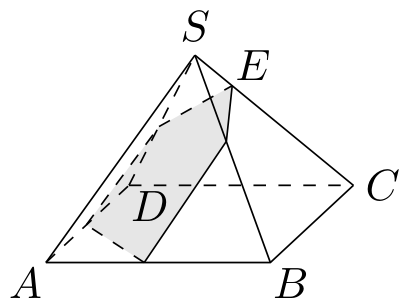
\includegraphics[width=4.9cm]{GaoKao/images/2012/jiangxi_science/q10_fig2.png}
\end{center}

        {\centering\begin{tabular*}{\linewidth}{@{}@{\extracolsep{\fill}}cccc@{}}
          \text{A. }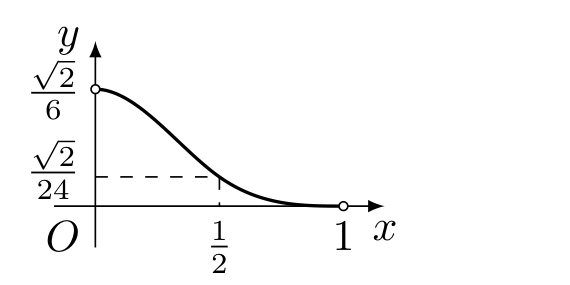
\includegraphics[width=0.15\paperwidth]{GaoKao/images/2012/jiangxi_science/q10_optA.png}  &  \text{B. }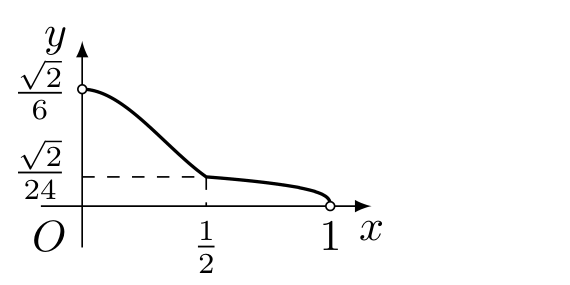
\includegraphics[width=0.15\paperwidth]{GaoKao/images/2012/jiangxi_science/q10_optB.png}  &  \text{C. }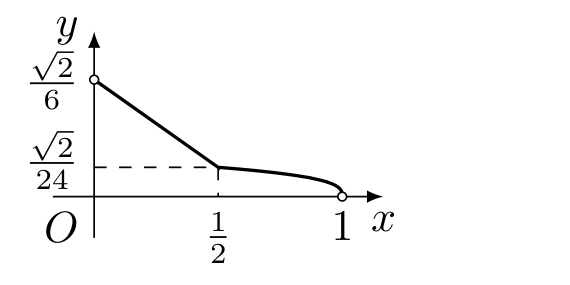
\includegraphics[width=0.15\paperwidth]{GaoKao/images/2012/jiangxi_science/q10_optC.png}  &  \text{D. }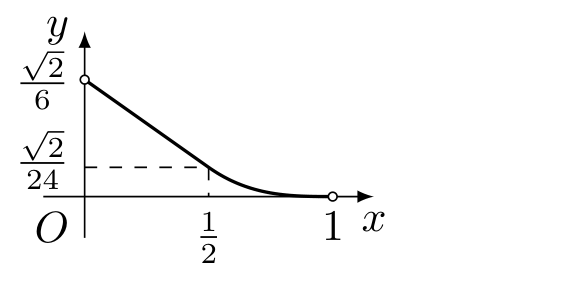
\includegraphics[width=0.15\paperwidth]{GaoKao/images/2012/jiangxi_science/q10_optD.png}
        \end{tabular*}\par}

    \end{enumerate}

\end{description}

\begin{description}

    \item[二、填空题]

    \begin{enumerate}[leftmargin=5pt]

      \addtocounter{enumi}{+10}

        \item 计算定积分 \(\int_{-1}^{1}\left(x^{2} + \sin x\right)\mathrm{d}x =\rule[-0.3ex]{3em}{0.4pt}\).

        \item 设数列 \(\{a_{n}\}\)，\(\{b_{n}\}\) 都是等差数列，若 \(a_{1} + b_{1} = 7\)，\(a_{3} + b_{3} = 21\)，则 \(a_{5} + b_{5} =\rule[-0.3ex]{3em}{0.4pt}\).

        \item 椭圆 \(\frac{x^{2}}{a^{2}} + \frac{y^{2}}{b^{2}} = 1\)（\(a > b > 0\)）的左、右顶点分别是 \(A\)，\(B\)，左、右焦点分别是 \(F_1\)，\(F_2\). 若 \(|AF_1|\)，\(|F_1F_2|\)，\(|F_1B|\) 成等比数列，则此椭圆的离心率为\rule[-0.3ex]{3em}{0.4pt}.

        \item 如图为某算法的程序框图，则程序运行后输出的结果是\rule[-0.3ex]{3em}{0.4pt}.

\begin{center}
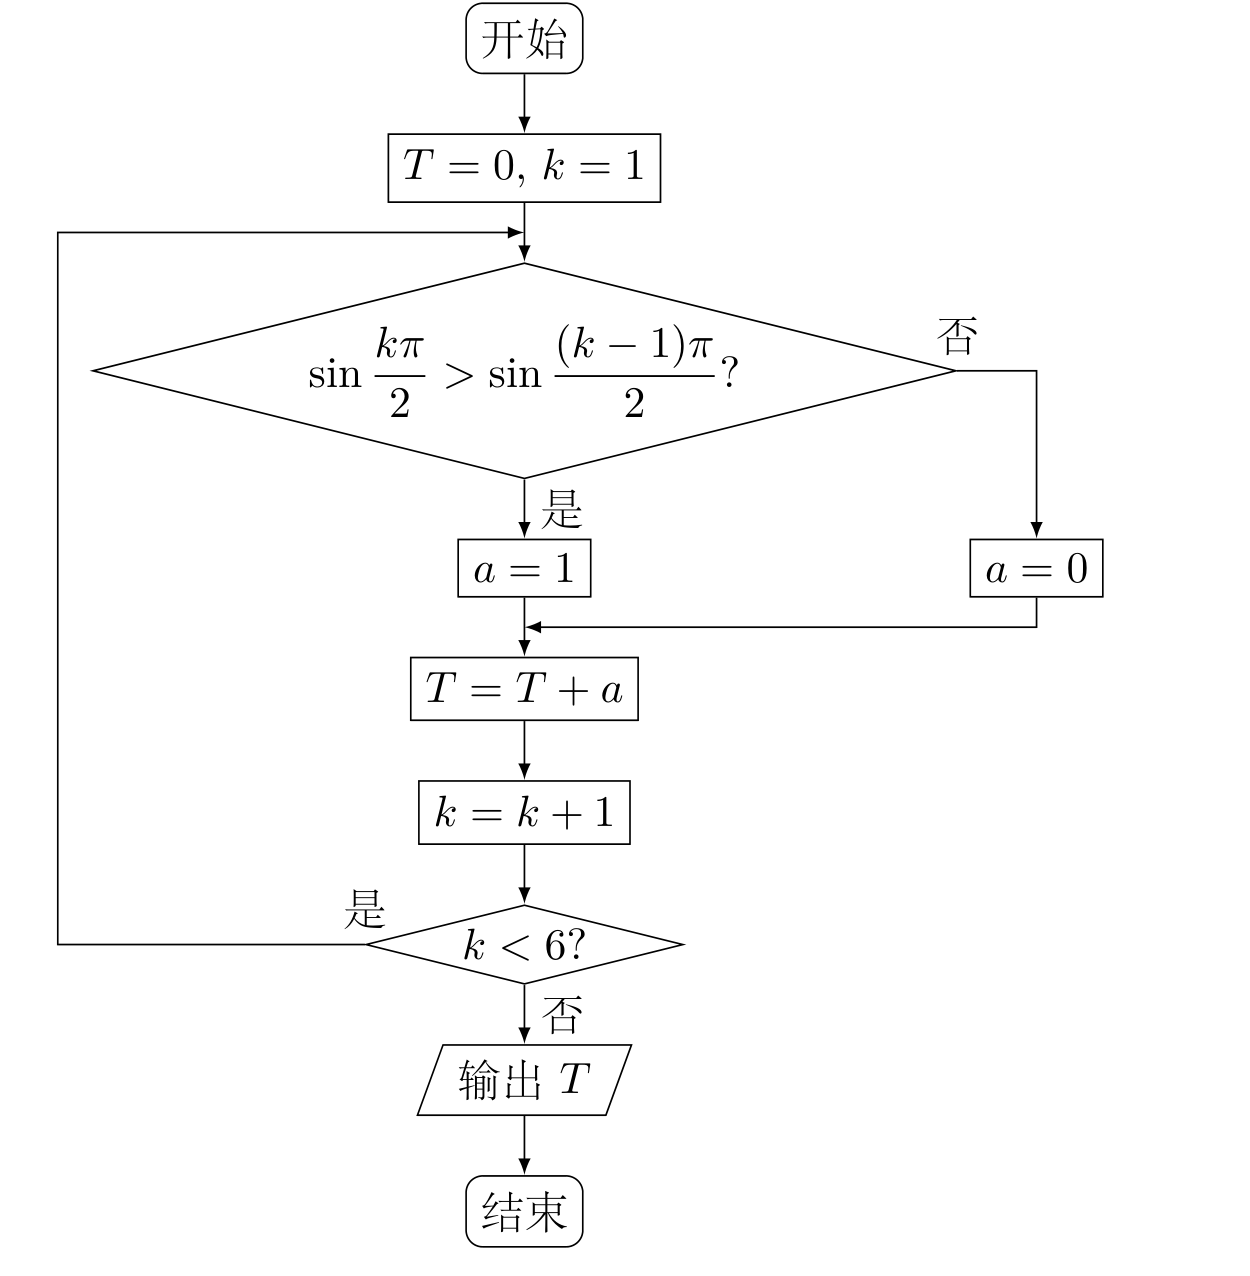
\includegraphics[width=0.62\linewidth]{GaoKao/images/2012/jiangxi_science/q14_flowchart.png}
\end{center}

    \end{enumerate}

\end{description}

\begin{description}

    \item[三、选做题]

    \begin{enumerate}[leftmargin=5pt]

      \addtocounter{enumi}{+14}

        \item \textbf{【选修4-4：坐标系与参数方程】}

曲线 \(C\) 的直角坐标方程为 \(x^{2} + y^{2} - 2x = 0\)，以原点为极点，\(x\) 轴的正半轴为极轴建立极坐标系，则曲线 \(C\) 的极坐标方程为\rule[-0.3ex]{3em}{0.4pt}.

        \item \textbf{【选修4-5：不等式选讲】}

在实数范围内，不等式 \(|2x - 1| + |2x + 1| \leqslant 6\) 的解集为\rule[-0.3ex]{3em}{0.4pt}.

    \end{enumerate}

\end{description}

\begin{description}

    \item[四、解答题]

    \begin{enumerate}[leftmargin=5pt]

      \addtocounter{enumi}{+16}

        \item 已知数列 \( \{a_{n}\} \) 的前 \(n\) 项和 \( S_{n} = -\frac{1}{2}n^{2} + kn \) （其中 \( k \in \mathbb{N}_{+} \) ），且 \( S_{n} \) 的最大值为 8.
\begin{enumerate}
\item 确定常数 \( k \)，并求 \( a_{n} \)；
\item 求数列 \( \left\{\frac{9-2a_{n}}{2^{n}}\right\} \) 的前 \(n\) 项和 \( T_{n} \).
\end{enumerate}

        \item 在 \(\triangle ABC\) 中，角 \(A\)，\(B\)，\(C\) 的对边分别为 \(a\)，\(b\)，\(c\). 已知 \(A = \frac{\pi}{4}\)，\(b \sin \left(\frac{\pi}{4} + C\right) - c \sin \left(\frac{\pi}{4} + B\right) = a\).
\begin{enumerate}
\item 求证： \(B - C = \frac{\pi}{2}\)；
\item 若 \(a = \sqrt{2}\)，求 \(\triangle ABC\) 的面积.
\end{enumerate}

        \item 如图，从 \(A_{1}(1,0,0)\)，\(A_{2}(2,0,0)\)，\(B_{1}(0,1,0)\)，\(B_{2}(0,2,0)\)，\(C_{1}(0,0,1)\)，\(C_{2}(0,0,2)\) 这6个点中随机选取3个点，将这3个点及原点 \(O\) 两两相连构成一个“立体”，记该“立体”的体积为随机变量 \(V\) （如果选取的3个点与原点在同一个平面内，此时“立体”的体积 \(V = 0\)）.
\begin{enumerate}
\item 求 \(V = 0\) 的概率；
\item 求 \(V\) 的分布列及数学期望 \(E(V)\).
\end{enumerate}

\begin{center}
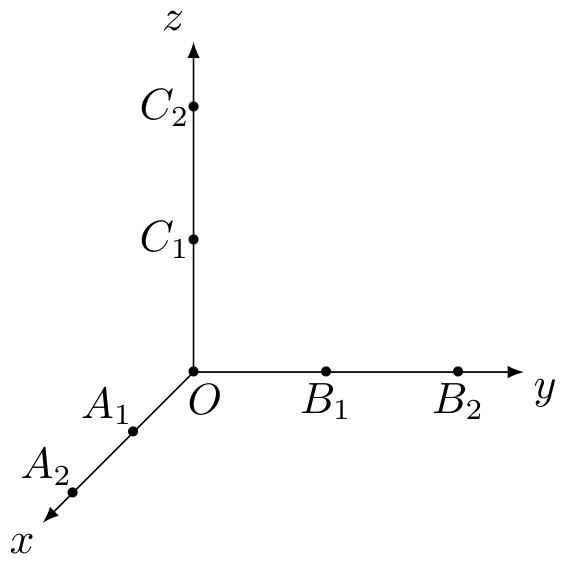
\includegraphics[width=5.6cm]{GaoKao/images/2012/jiangxi_science/q19_fig1.png}
\end{center}

        \item 在三棱柱 \(ABC - A_{1}B_{1}C_{1}\) 中，已知 \(AB = AC = AA_{1} = \sqrt{5}\)，\(BC = 4\)，点 \(A_{1}\) 在底面 \(ABC\) 的射影是线段 \(BC\) 的中点 \(O\).
\begin{enumerate}
\item 证明：在侧棱 \(AA_{1}\) 上存在一点 \(E\)，使得 \(OE \perp \) 平面 \(BB_{1}C_{1}C\)，并求出 \(AE\) 的长；
\item 求平面 \(A_{1}B_{1}C\) 与平面 \(BB_{1}C_{1}C\) 夹角的余弦值.
\end{enumerate}

\begin{center}
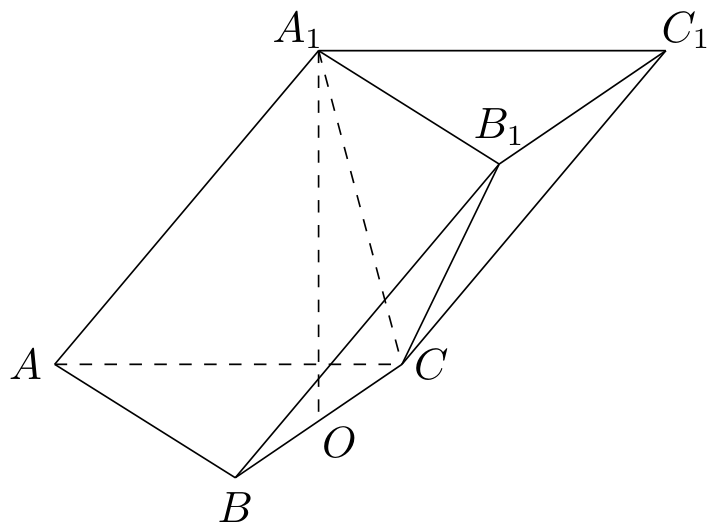
\includegraphics[width=7.5cm]{GaoKao/images/2012/jiangxi_science/q20_fig1.png}
\end{center}

        \item 已知三点 \(O(0,0)\)，\(A(-2,1)\)，\(B(2,1)\)，曲线 \(C\) 上任意一点 \(M(x,y)\) 满足 \(\left|\overrightarrow{MA} + \overrightarrow{MB}\right| = \overrightarrow{OM} \cdot \left(\overrightarrow{OA} + \overrightarrow{OB}\right) + 2\).
\begin{enumerate}
\item 求曲线 \(C\) 的方程；
\item 动点 \(Q(x_0, y_0)\) （\(-2 < x_0 < 2\)）在曲线 \(C\) 上，曲线 \(C\) 在点 \(Q\) 处的切线为 \(l\). 问：是否存在定点 \(P(0, t)\) （\(t < 0\)），使得 \(l\) 与 \(PA\)，\(PB\) 都相交，交点分别为 \(D\)，\(E\)，且 \(\triangle QAB\) 与 \(\triangle PDE\) 的面积之比是常数？若存在，求 \(t\) 的值；若不存在，请说明理由.
\end{enumerate}

        \item 若函数 \(h(x)\) 满足
\begin{enumerate}
\item \(h(0)=1\)，\(h(1)=0\)；
\item 对任意 \(a \in [0,1]\)，有 \(h(h(a)) = a\)；
\item 在 \((0,1)\) 上单调递减.
\end{enumerate}
则称 \(h(x)\) 为补函数. 已知函数 \(h(x) = \left(\frac{1 - x^{p}}{1 + \lambda x^{p}}\right)^{\frac{1}{p}}\)（\(\lambda > -1\)，\(p > 0\)）.
\begin{enumerate}
\item 判断函数 \(h(x)\) 是否为补函数，并证明你的结论；
\item 若存在 \(m \in [0,1]\)，使得 \(h(m) = m\)，称 \(m\) 是函数 \(h(x)\) 的中介元. 记 \(p = \frac{1}{n} \) （\(n \in \mathbf{N}_+\)）时 \(h(x)\) 的中介元为 \(x_n\). 且 \(S_n = \sum_{i=1}^{n} x_i\)，若对任意的 \(n \in \mathbf{N}_+\)，都有 \(S_n < \frac{1}{2}\)，求 \(\lambda\) 的取值范围；
\item 当 \(\lambda = 0\)，\(x \in (0,1)\) 时，函数 \(y = h(x)\) 的图象总在直线 \(y = 1 - x\) 的上方，求 \(p\) 的取值范围.
\end{enumerate}

    \end{enumerate}

\end{description}


\subsection{2012年江西卷（文）}\label{gk:2012年江西卷（文）}

\begin{description}

    \item[一、选择题]

    \begin{enumerate}[leftmargin=5pt]

        \item 若复数 \(z = 1 + \i\) （\(\i\) 为虚数单位），\(\overline{z}\) 是 \(z\) 的共轭复数，则 \(z^2 + \overline{z}^2\) 的虚部为（\quad）

        {\centering\begin{tabular*}{\linewidth}{@{}@{\extracolsep{\fill}}llll@{}}
          \text{A. }0  &  \text{B. }\(-1\)  &  \text{C. }1  &  \text{D. }\(-2\)
        \end{tabular*}\par}

        \item 若全集 \(U = \{x \in \mathbb{R} \mid x^2 \leqslant 4\}\)，则集合 \(A = \{x \in \mathbb{R} \mid |x + 1| \leqslant 1\}\) 的补集 \(\complement_U A\) 为（\quad）

        {\centering\begin{tabular*}{\linewidth}{@{}@{\extracolsep{\fill}}llll@{}}
          \text{A. }\(\{x\in \mathbb{R}\mid 0 < x < 2\}\)  &  \text{B. }\(\{x\in \mathbb{R}\mid 0\leqslant x < 2\}\)  &  \text{C. }\(\{x\in \mathbb{R}\mid 0 < x\leqslant 2\}\)  &  \text{D. }\(\{x\in \mathbb{R}\mid 0\leqslant x\leqslant 2\}\)
        \end{tabular*}\par}

        \item 设函数 \( f(x) = \begin{cases}
x^2 + 1, & x \leqslant 1,\\
\frac{2}{x}, & x > 1,
\end{cases} \) 则 \( f(f(3)) = \)（\quad）

        {\centering\begin{tabular*}{\linewidth}{@{}@{\extracolsep{\fill}}llll@{}}
          \text{A. }\(\frac{1}{5}\)  &  \text{B. }3  &  \text{C. }\( \frac{2}{3} \)  &  \text{D. }\(\frac{13}{9}\)
        \end{tabular*}\par}

        \item 若 \(\frac{\sin\alpha + \cos\alpha}{\sin\alpha - \cos\alpha} = \frac{1}{2}\)，则 \(\tan 2\alpha =\)（\quad）

        {\centering\begin{tabular*}{\linewidth}{@{}@{\extracolsep{\fill}}llll@{}}
          \text{A. }\(-\frac{3}{4}\)  &  \text{B. }\( \frac{3}{4} \)  &  \text{C. }\(-\frac{4}{3}\)  &  \text{D. }\(\frac{4}{3}\)
        \end{tabular*}\par}

        \item 观察下列事实： \(|x| + |y| = 1\) 的不同整数解 \((x, y)\) 的个数为 4，\(|x| + |y| = 2\) 的不同整数解 \((x, y)\) 的个数为 8，\(|x| + |y| = 3\) 的不同整数解 \((x, y)\) 的个数为 12，\(\cdots\)，则 \(|x| + |y| = 20\) 的不同整数解 \((x, y)\) 的个数为（\quad）

        {\centering\begin{tabular*}{\linewidth}{@{}@{\extracolsep{\fill}}llll@{}}
          \text{A. }76  &  \text{B. }80  &  \text{C. }86  &  \text{D. }92
        \end{tabular*}\par}

        \item 小波一星期的总开支分布如图 1 所示，一星期的食品开支如图 2 所示，则小波一星期的鸡蛋开支占总开支的百分比为（\quad）

\begin{center}
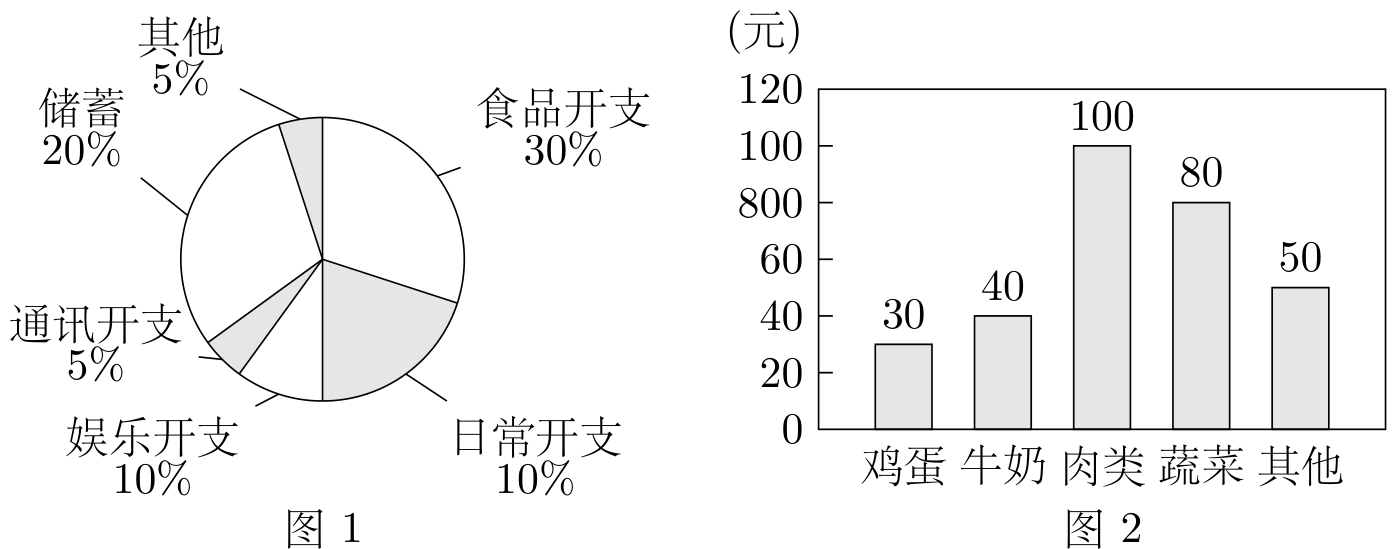
\includegraphics[width=13.4cm]{GaoKao/images/2012/jiangxi_liberal/q6_fig1.png}
\end{center}

        {\centering\begin{tabular*}{\linewidth}{@{}@{\extracolsep{\fill}}llll@{}}
          \text{A. }30\%  &  \text{B. }10\%  &  \text{C. }3\%  &  \text{D. }不能确定
        \end{tabular*}\par}

        \item 若一个几何体的三视图如图所示，则此几何体的体积为（\quad）

\begin{center}
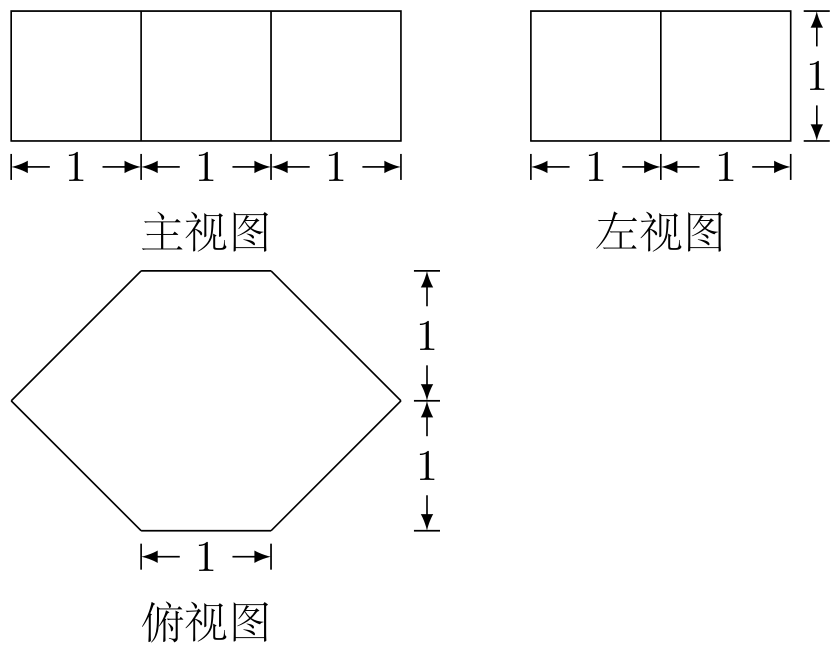
\includegraphics[width=8.7cm]{GaoKao/images/2012/jiangxi_liberal/q7_fig1.png}
\end{center}

        {\centering\begin{tabular*}{\linewidth}{@{}@{\extracolsep{\fill}}llll@{}}
          \text{A. }\(\frac{11}{2}\)  &  \text{B. }5  &  \text{C. }\(\frac{9}{2}\)  &  \text{D. }4
        \end{tabular*}\par}

        \item 椭圆 \(\frac{x^2}{a^2} + \frac{y^2}{b^2} = 1\) （\(a > b > 0\)）的左、右顶点分别是 \(A\)，\(B\)，左、右焦点分别是 \(F_1\)，\(F_2\). 若 \(|AF_1|\)，\(|F_1F_2|\)，\(|F_1B|\) 成等比数列，则此椭圆的离心率为（\quad）

        {\centering\begin{tabular*}{\linewidth}{@{}@{\extracolsep{\fill}}llll@{}}
          \text{A. }\(\frac{1}{4}\)  &  \text{B. }\(\frac{\sqrt{5}}{5}\)  &  \text{C. }\(\frac{1}{2}\)  &  \text{D. }\(\sqrt{5} - 2\)
        \end{tabular*}\par}

        \item 已知 \( f(x) = \sin^2\left(x + \frac{\pi}{4}\right) \). 若 \(a = f(\lg 5)\)，\(b = f\left(\lg \frac{1}{5}\right)\)，则（\quad）

        {\centering\begin{tabular*}{\linewidth}{@{}@{\extracolsep{\fill}}llll@{}}
          \text{A. }\( a + b = 0 \)  &  \text{B. }\( a - b = 0 \)  &  \text{C. }\( a + b = 1 \)  &  \text{D. }\( a - b = 1 \)
        \end{tabular*}\par}

        \item 如图，\(|OA| = 2 \mathrm{~m}\)，\(|OB| = 1 \mathrm{~m}\)，\(OA\) 与 \(OB\) 的夹角为 \(\frac{\pi}{6}\)，以 \(A\) 为圆心，\(AB\) 为半径作圆弧 \(BDC\) 与线段 \(OA\) 的延长线交于点 \(C\). 甲、乙两质点同时从点 \(O\) 出发，甲先以速率 \(1 \mathrm{~m/s}\) 沿线段 \(OB\) 行至点 \(B\)，再以速率 \(3 \mathrm{~m/s}\) 沿圆弧 \(BDC\) 行至点 \(C\) 后停止；乙以速率 \(2 \mathrm{~m/s}\) 沿线段 \(OA\) 行至点 \(A\) 后停止. 设 \(t\) 时刻甲、乙两点连线与它们经过的路径所围成图形的面积为 \(S(t)\)（\(S(0)=0\)），则函数 \(y = S(t)\) 的图象大致是（\quad）

\begin{center}
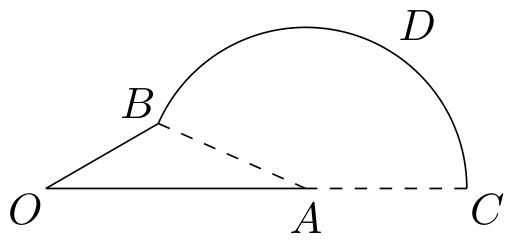
\includegraphics[width=6.2cm]{GaoKao/images/2012/jiangxi_liberal/q10_fig2.png}
\end{center}

        {\centering\begin{tabular*}{\linewidth}{@{}@{\extracolsep{\fill}}cccc@{}}
          \text{A. }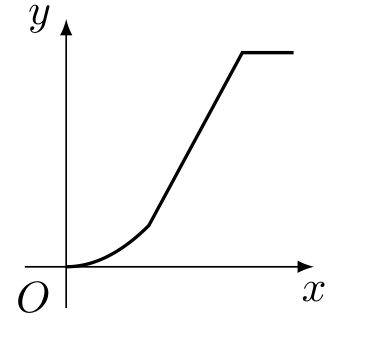
\includegraphics[width=0.15\paperwidth]{GaoKao/images/2012/jiangxi_liberal/q10_optA.png}  &  \text{B. }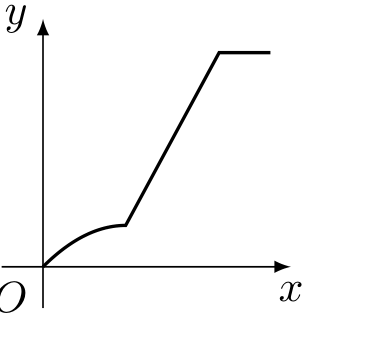
\includegraphics[width=0.15\paperwidth]{GaoKao/images/2012/jiangxi_liberal/q10_optB.png}  &  \text{C. }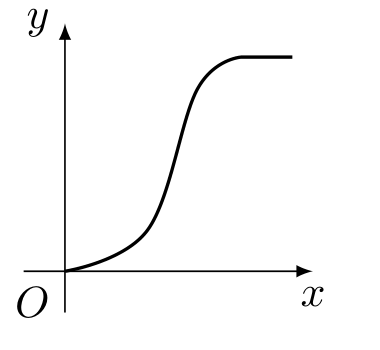
\includegraphics[width=0.15\paperwidth]{GaoKao/images/2012/jiangxi_liberal/q10_optC.png}  &  \text{D. }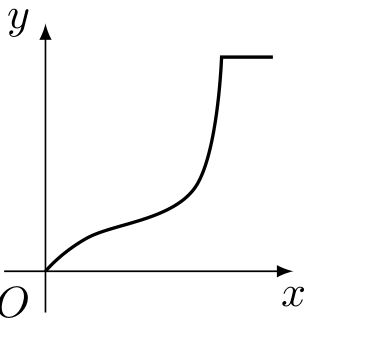
\includegraphics[width=0.15\paperwidth]{GaoKao/images/2012/jiangxi_liberal/q10_optD.png}
        \end{tabular*}\par}

    \end{enumerate}

\end{description}

\begin{description}

    \item[二、填空题]

    \begin{enumerate}[leftmargin=5pt]

      \addtocounter{enumi}{+10}

        \item 不等式 \(\frac{x^2 - 9}{x - 2} > 0\) 的解集是\rule[-0.3ex]{3em}{0.4pt}.

        \item 设单位向量 \(\bm{m} = (x, y)\)，\(\bm{b} = (2, -1)\). 若 \(\bm{m} \perp \bm{b}\)，则 \(|x + 2y| = \)\rule[-0.3ex]{3em}{0.4pt}.

        \item 等比数列 \(\{a_{n}\}\) 的前 \(n\) 项和为 \(S_{n}\)，公比不为 1. 若 \(a_{1} = 1\)，且对任意的 \(n \in \mathbf{N}^{*}\)，都有 \(a_{n+2} + a_{n+1} - 2a_{n} = 0\)，则 \(S_{5} = \)\rule[-0.3ex]{3em}{0.4pt}.

        \item 过直线 \(x + y - 2\sqrt{2} = 0\) 上的点 \(P\) 作圆 \(x^{2} + y^{2} = 1\) 的两条切线，若两条切线的夹角是 \(60^{\circ}\)，则点 \(P\) 的坐标是\rule[-0.3ex]{3em}{0.4pt}.

        \item 如图为某算法的程序框图，则程序运行后输出的结果是\rule[-0.3ex]{3em}{0.4pt}.

\begin{center}
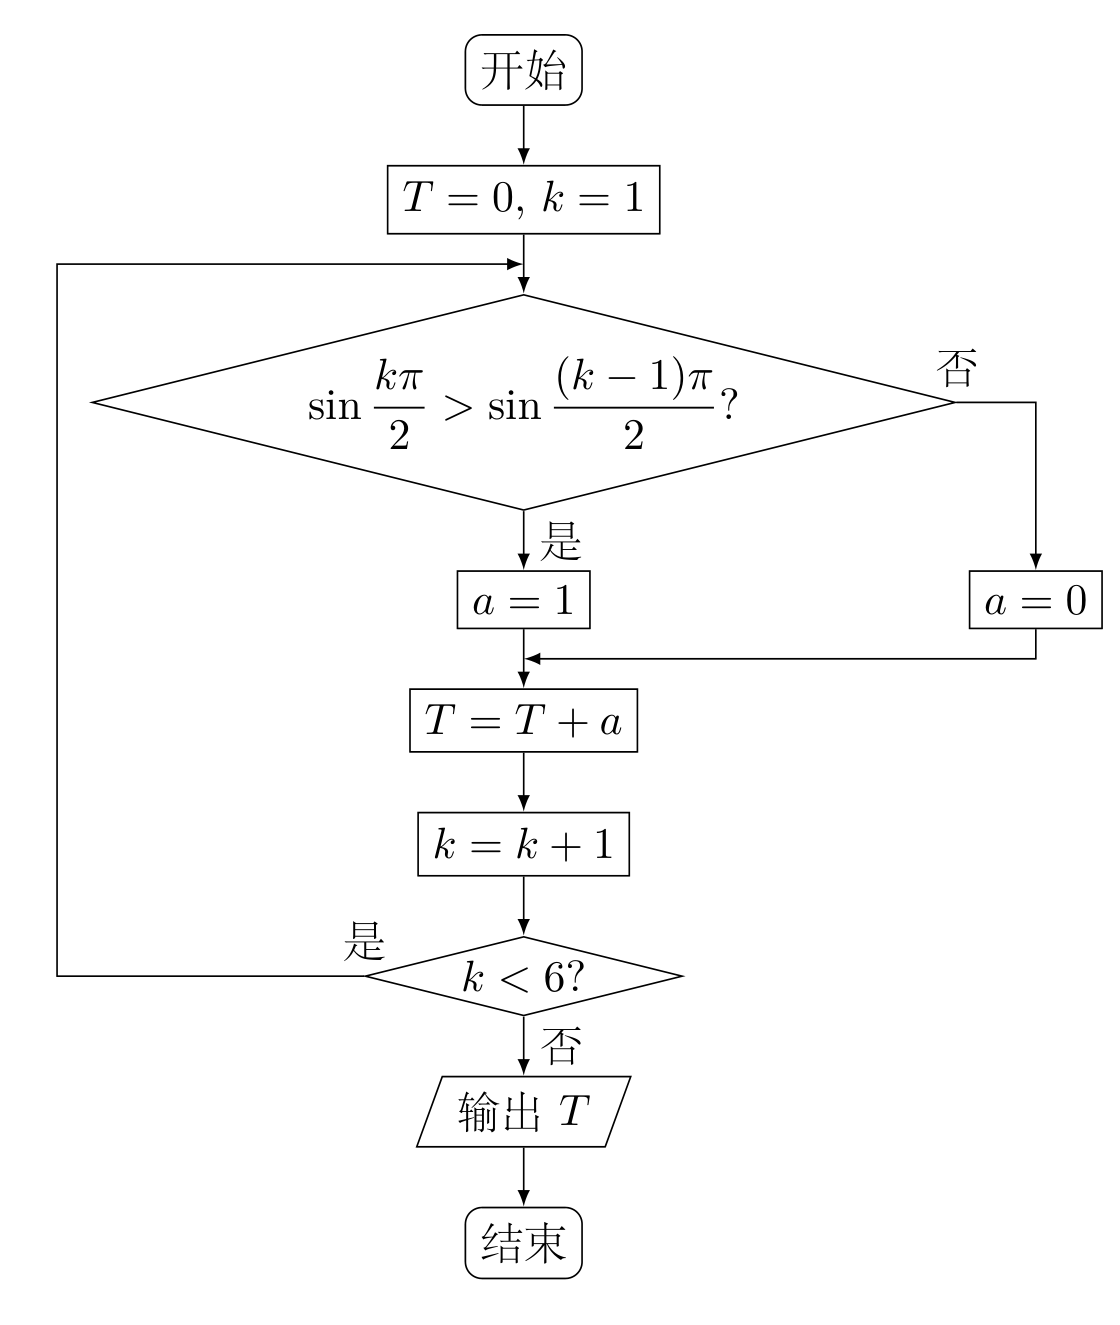
\includegraphics[width=5.5cm]{GaoKao/images/2012/jiangxi_liberal/q15_fig1.png}
\end{center}

    \end{enumerate}

\end{description}

\begin{description}

    \item[三、解答题]

    \begin{enumerate}[leftmargin=5pt]

      \addtocounter{enumi}{+15}

        \item 在 \(\triangle ABC\) 中，角 \(A\)，\(B\)，\(C\) 的对边分别为 \(a\)，\(b\)，\(c\). 已知 \(3\cos (B - C) - 1 = 6\cos B\cos C\).
\begin{enumerate}
\item 求 \( \cos A \)；
\item 若 \(a = 3\)，\(\triangle ABC\) 的面积为 \(2\sqrt{2}\)，求 \(b\)，\(c\).
\end{enumerate}

        \item 已知数列 \(\{a_{n}\}\) 的前 \(n\) 项和 \(S_{n} = kc^{n} - k\) （其中 \(c\)，\(k\) 为常数），且 \(a_{2} = 4\)，\(a_{6} = 8a_{3}\).
\begin{enumerate}
\item 求 \(a_{n}\)；
\item 求数列 \( \{na_{n}\} \) 的前 \(n\) 项和 \( T_{n} \).
\end{enumerate}

        \item 如图，从 \(A_{1}(1,0,0)\)，\(A_{2}(2,0,0)\)，\(B_{1}(0,1,0)\)，\(B_{2}(0,2,0)\)，\(C_{1}(0,0,1)\)，\(C_{2}(0,0,2)\) 这 6 个点中随机选取 3 个点.
\begin{enumerate}
\item 求这 3 点与原点 \(O\) 恰好是正三棱锥的四个顶点的概率；
\item 求这 3 点与原点 \(O\) 共面的概率.
\end{enumerate}

\begin{center}
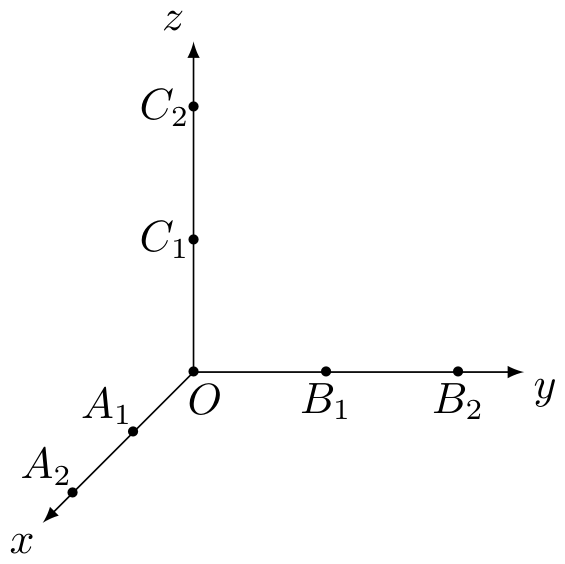
\includegraphics[width=5.6cm]{GaoKao/images/2012/jiangxi_liberal/q18_fig1.png}
\end{center}

        \item 如图，在梯形 \(ABCD\) 中，\(AB \parallel CD\)，\(E\)，\(F\) 是线段 \(AB\) 上的两点，且 \(DE \perp AB\)，\(CF \perp AB\)，\(AB = 12\)，\(AD = 5\)，\(BC = 4\sqrt{2}\)，\(DE = 4\). 现将 \(\triangle ADE\)，\(\triangle CFB\) 分别沿 \(DE\)，\(CF\) 折起，使 \(A\)，\(B\) 两点重合于点 \(G\)，得到多面体 \(CDEFG\).
\begin{enumerate}
\item 求证：平面 \(DEG \perp\) 平面 \(CFG\)；
\item 求多面体 \(CDEFG\) 的体积.
\end{enumerate}

\begin{center}
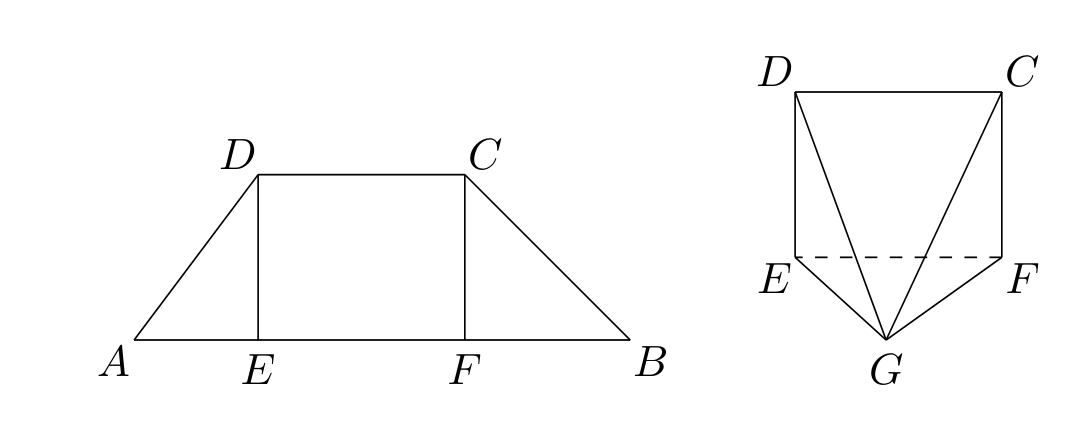
\includegraphics[width=16.0cm]{GaoKao/images/2012/jiangxi_liberal/q19_fig1.png}
\end{center}

        \item 已知函数 \( f(x) = (ax^2 + bx + c){\mathrm{e}}^x \) 在 \([0,1]\) 上单调递减且满足 \( f(0) = 1 \)，\( f(1) = 0 \).
\begin{enumerate}
\item 求 \(a\) 的取值范围；
\item 设 \( g(x) = f(x) - f'(x) \)，求 \(g(x)\) 在 \([0,1]\) 上的最大值和最小值.
\end{enumerate}

        \item 已知三点 \(O(0,0)\)，\(A(-2,1)\)，\(B(2,1)\)，曲线 \(C\) 上任意一点 \(M(x,y)\) 满足 \(\left|\overrightarrow{MA} + \overrightarrow{MB}\right| = \overrightarrow{OM} \cdot \left(\overrightarrow{OA} + \overrightarrow{OB}\right) + 2\).
\begin{enumerate}
\item 求曲线 \(C\) 的方程；
\item 点 \(Q(x_0, y_0)\) （\(-2 < x_0 < 2\)） 是曲线 \(C\) 上的动点，曲线 \(C\) 在点 \(Q\) 处的切线为 \(l\)，点 \(P\) 的坐标是 \((0, -1)\)，\(l\) 与 \(PA\)，\(PB\) 分别交于点 \(D\)，\(E\)，求 \(\triangle QAB\) 与 \(\triangle PDE\) 的面积之比.
\end{enumerate}

    \end{enumerate}

\end{description}


\subsection{2012年辽宁卷（理）}\label{gk:2012年辽宁卷（理）}

\begin{description}

    \item[一、选择题]

    \begin{enumerate}[leftmargin=5pt]

        \item 已知全集 \(U = \{0, 1, 2, 3, 4, 5, 6, 7, 8, 9\}\)，集合 \(A = \{0, 1, 3, 5, 8\}\)，集合 \(B = \{2, 4, 5, 6, 8\}\)，则 \((\complement_U A) \cap (\complement_U B) =\)（\quad）

        {\centering\begin{tabular*}{\linewidth}{@{}@{\extracolsep{\fill}}llll@{}}
          \text{A. }\(\{5,8\}\)  &  \text{B. }\(\{7,9\}\)  &  \text{C. }\(\{0,1,3\}\)  &  \text{D. }\(\{2,4,6\}\)
        \end{tabular*}\par}

        \item 复数 \(\frac{2 - \i}{2 + \i} =\)（\quad）

        {\centering\begin{tabular*}{\linewidth}{@{}@{\extracolsep{\fill}}llll@{}}
          \text{A. }\(\frac{3}{5} - \frac{4}{5}\i\)  &  \text{B. }\(\frac{3}{5} + \frac{4}{5}\i\)  &  \text{C. }\(1 - \frac{4}{5}\i\)  &  \text{D. }\(1 + \frac{3}{5}\i\)
        \end{tabular*}\par}

        \item 已知两个非零向量 \(\bm{a}\)，\(\bm{b}\) 满足 \(|\bm{a} + \bm{b}| = |\bm{a} - \bm{b}|\). 则下面结论正确的是（\quad）

        {\centering\begin{tabular*}{\linewidth}{@{}@{\extracolsep{\fill}}llll@{}}
          \text{A. }\(\bm{a} \parallel \bm{b}\)  &  \text{B. }\(\bm{a} \perp \bm{b}\)  &  \text{C. }\(|\bm{a}| = |\bm{b}|\)  &  \text{D. }\(\bm{a} + \bm{b} = \bm{a} - \bm{b}\)
        \end{tabular*}\par}

        \item 已知命题 \(p: \forall x_1,x_2 \in \mathbb{R}\)，\((f(x_2) - f(x_1))(x_2 - x_1) \geqslant 0\)，则 \(\neg p\) 是（\quad）

        {\centering\begin{tabular*}{\linewidth}{@{}@{\extracolsep{\fill}}llll@{}}
          \text{A. }\(\exists x_{1}, x_{2} \in \mathbb{R}, (f(x_{2}) - f(x_{1}))(x_{2} - x_{1}) \leqslant 0\)  &  \text{B. }\(\forall x_{1},x_{2} \in \mathbb{R},\ (f(x_{2}) - f(x_{1}))(x_{2} - x_{1}) \leqslant 0\)  &  \text{C. }\(\exists x_{1},x_{2} \in \mathbb{R},\ (f(x_{2}) - f(x_{1}))(x_{2} - x_{1}) < 0\)  &  \text{D. }\(\forall x_{1},x_{2} \in \mathbb{R},\ (f(x_{2}) - f(x_{1}))(x_{2} - x_{1}) < 0\)
        \end{tabular*}\par}

        \item 一排\(9\) 个座位坐了\(3\) 个三口之家，若每家人坐在一起，则不同的坐法种数（\quad）

        {\centering\begin{tabular*}{\linewidth}{@{}@{\extracolsep{\fill}}llll@{}}
          \text{A. }\(3 \times 3!\)  &  \text{B. }\(3 \times (3!)^{3}\)  &  \text{C. }\((3!)^{4}\)  &  \text{D. }\(9! \)
        \end{tabular*}\par}

        \item 在等差数列 \(\{a_{n}\}\) 中，已知 \(a_{4} + a_{8} = 16\)，则该数列前 \(11\) 项和 \(S_{11} =\)（\quad）

        {\centering\begin{tabular*}{\linewidth}{@{}@{\extracolsep{\fill}}llll@{}}
          \text{A. }58  &  \text{B. }88  &  \text{C. }143  &  \text{D. }176
        \end{tabular*}\par}

        \item 已知 \(\sin \alpha - \cos \alpha = \sqrt{2}\)，\(\alpha \in (0, \pi)\)，则 \(\tan \alpha =\)（\quad）

        {\centering\begin{tabular*}{\linewidth}{@{}@{\extracolsep{\fill}}llll@{}}
          \text{A. }\(-1\)  &  \text{B. }\(-\frac{\sqrt{2}}{2}\)  &  \text{C. }\(\frac{\sqrt{2}}{2}\)  &  \text{D. }1
        \end{tabular*}\par}

        \item 设变量 \(x\)，\(y\) 满足 \(\begin{cases}
x - y \leqslant 10,\\
0 \leqslant x + y \leqslant 20,\\
0 \leqslant y \leqslant 15,
\end{cases}\) 则 \(2x + 3y\) 的最大值为（\quad）

        {\centering\begin{tabular*}{\linewidth}{@{}@{\extracolsep{\fill}}llll@{}}
          \text{A. }20  &  \text{B. }35  &  \text{C. }45  &  \text{D. }55
        \end{tabular*}\par}

        \item 执行如图所示的程序框图，则输出的 \(S\) 值是（\quad）

\begin{center}
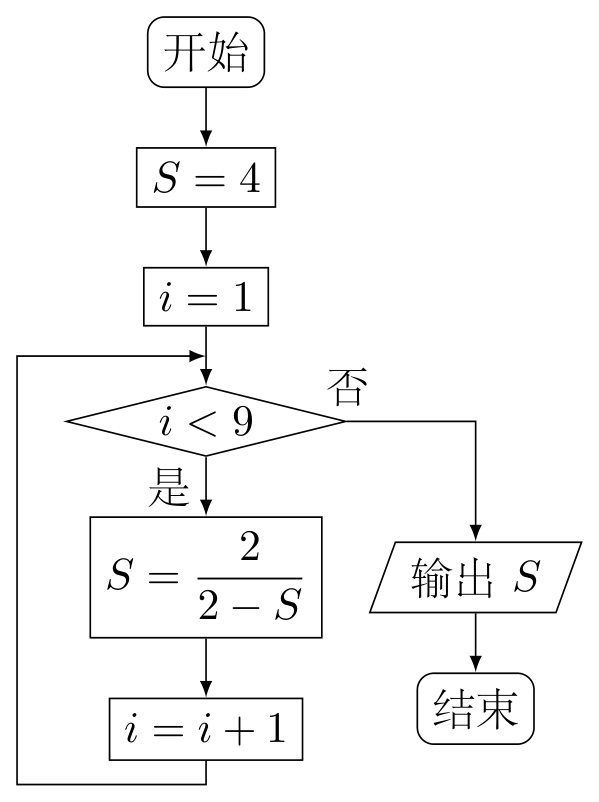
\includegraphics[width=0.55\linewidth]{GaoKao/images/2012/liaoning_science/q9_fig1.png}
\end{center}

        {\centering\begin{tabular*}{\linewidth}{@{}@{\extracolsep{\fill}}llll@{}}
          \text{A. }\(-1\)  &  \text{B. }\( \frac{3}{2} \)  &  \text{C. }\( \frac{2}{3} \)  &  \text{D. }4
        \end{tabular*}\par}

        \item 在长为 \(12 \mathrm{~cm}\) 的线段 \(AB\) 上任取一点 \(C\). 现作一矩形，邻边长分别等于线段 \(AC\)，\(CB\) 的长，则该矩形面积小于 \(32 \mathrm{~cm}^{2}\) 的概率为（\quad）

        {\centering\begin{tabular*}{\linewidth}{@{}@{\extracolsep{\fill}}llll@{}}
          \text{A. }\(\frac{1}{6}\)  &  \text{B. }\( \frac{1}{3} \)  &  \text{C. }\( \frac{2}{3} \)  &  \text{D. }\( \frac{4}{5} \)
        \end{tabular*}\par}

        \item 设函数 \(f(x)\)（\(x \in \mathbb{R}\)）满足 \(f(-x) = f(x)\)，\(f(x) = f(2 - x)\)，且当 \(x \in [0,1]\) 时，\(f(x) = x^3\). 又函数 \(g(x) = |x\cos(\pi x)|\)，则函数 \(h(x) = g(x) - f(x)\) 在 \(\left[-\frac{1}{2}, \frac{3}{2}\right]\) 上的零点个数为（\quad）

        {\centering\begin{tabular*}{\linewidth}{@{}@{\extracolsep{\fill}}llll@{}}
          \text{A. }5  &  \text{B. }6  &  \text{C. }7  &  \text{D. }8
        \end{tabular*}\par}

        \item 若 \(x \in [0, +\infty)\)，则下列不等式恒成立的是（\quad）

        {\centering\begin{tabular*}{\linewidth}{@{}@{\extracolsep{\fill}}llll@{}}
          \text{A. }\( {\mathrm{e}}^{x}\leqslant1+x+x^{2} \)  &  \text{B. }\(\frac{1}{\sqrt{1 + x}}\leqslant 1 - \frac{1}{2} x + \frac{1}{4} x^2\)  &  \text{C. }\(\cos x \geqslant 1 - \frac{1}{2} x^2\)  &  \text{D. }\(\ln (1 + x) \geqslant x - \frac{1}{8} x^2\)
        \end{tabular*}\par}

    \end{enumerate}

\end{description}

\begin{description}

    \item[二、填空题]

    \begin{enumerate}[leftmargin=5pt]

      \addtocounter{enumi}{+12}

        \item 一个几何体的三视图如图所示，则该几何体的表面积为\rule[-0.3ex]{3em}{0.4pt}.

\begin{center}
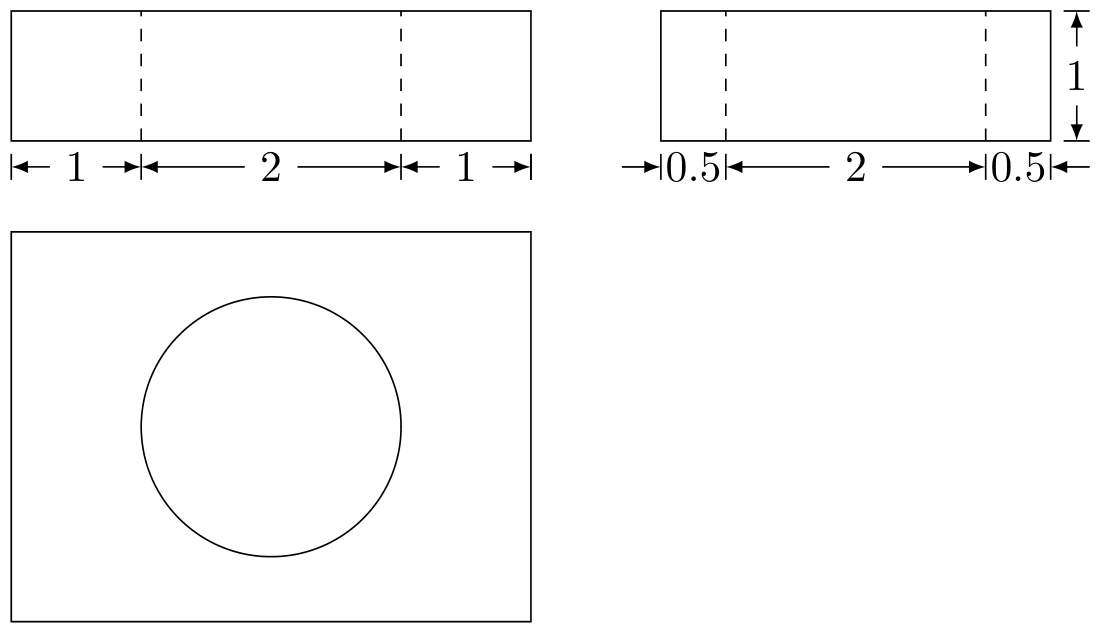
\includegraphics[width=11.0cm]{GaoKao/images/2012/liaoning_science/q13_fig1.png}
\end{center}

        \item 已知等比数列 \( \{a_{n}\} \) 为递增数列，且 \(a_{3}^{2}=a_{10}\)，\(2(a_{n}+a_{n+2})=5a_{n+1}\)，则数列 \( \{a_{n}\} \) 的通项公式 \( a_{n}= \)\rule[-0.3ex]{3em}{0.4pt}.

        \item 已知 \(P\)，\(Q\) 为抛物线 \(x^{2} = 2y\) 上两点，点 \(P\)，\(Q\) 的横坐标分别为 4，\(-2\)，过 \(P\)，\(Q\) 分别作抛物线的切线. 两切线交于 \(A\)，则点 \(A\) 的纵坐标为\rule[-0.3ex]{3em}{0.4pt}.

        \item 已知正三棱锥 \(P - ABC\)，点 \(P\)，\(A\)，\(B\)，\(C\) 都在半径为 \(\sqrt{3}\) 的球面上. 若 \(PA\)，\(PB\)，\(PC\) 两两互相垂直，则球心到截面 \(ABC\) 的距离为\rule[-0.3ex]{3em}{0.4pt}.

    \end{enumerate}

\end{description}

\begin{description}

    \item[三、解答题]

    \begin{enumerate}[leftmargin=5pt]

      \addtocounter{enumi}{+16}

        \item 在 \(\triangle ABC\) 中，角 \(A\)，\(B\)，\(C\) 的对边分别为 \(a\)，\(b\)，\(c\). 角 \(A\)，\(B\)，\(C\) 成等差数列.

\begin{enumerate}
\item 求 \(\cos B\) 的值.
\item 若边 \(a\)，\(b\)，\(c\) 成等比数列，求 \(\sin A \sin C\) 的值.
\end{enumerate}

        \item 如图，直三棱柱 \(ABC - A'B'C'\)，\(\angle BAC = 90^\circ\)，\(AB = AC = \lambda AA'\)，点 \(M\)，\(N\) 分别为 \(A'B\) 和 \(B'C'\) 的中点.

\begin{enumerate}
\item 证明：\(MN \parallel\) 平面 \(A'ACC'\).
\item 若二面角 \(A' - MN - C\) 为直二面角，求 \(\lambda\) 的值.
\end{enumerate}

\begin{center}
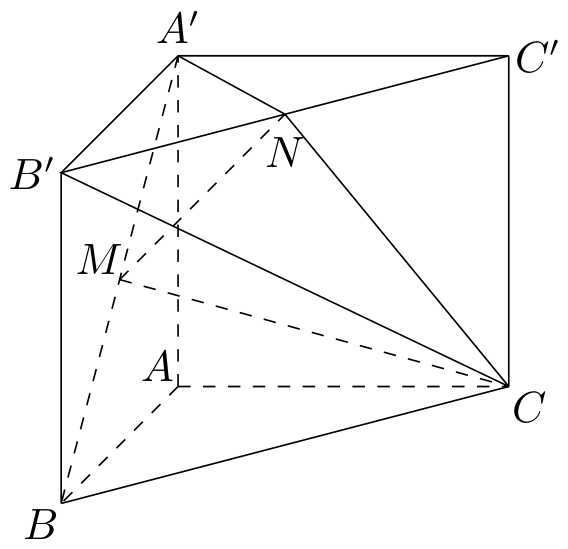
\includegraphics[width=6.6cm]{GaoKao/images/2012/liaoning_science/q18_fig1.png}
\end{center}

        \item 电视传媒公司为了解某地区电视观众对某类体育节目的收视情况，随机抽取了 \(100\) 名观众进行调查. 下面是根据调查结果绘制的观众日均收看该体育节目时间的频率分布直方图：

将日均收看该体育节目时间不低于 \(40\) 分钟的观众称为“体育迷”.

\begin{enumerate}
\item 根据已知条件完成下面的 \(2 \times 2\) 列表，并据此资料你是否认为“体育迷”与性别有关？

\begin{center}
\begin{tabular}{|c|c|c|c|}
\hline
 & 非体育迷 & 体育迷 & 合计 \\
\hline
男 &  &  &  \\
\hline
女 &  & \(10\) & \(55\) \\
\hline
合计 &  &  &  \\
\hline
\end{tabular}
\end{center}

\item 将上述调查所得到的频率视为概率. 现在从该地区大量电视观众中，采用随机抽样方法每次抽取一名观众. 抽取 \(3\) 次，记被抽取的 \(3\) 名观众中的“体育迷”人数为 \(X\). 若每次抽取的结果是相互独立的，求 \(X\) 的分布列，期望 \(E(X)\) 和方差 \(D(X)\).
\end{enumerate}

附：\(\chi^2 = \dfrac{n(ad-bc)^2}{(a+b)(c+d)(a+c)(b+d)}\)，\(P(\chi^2 \geqslant k)\) 与 \(k\) 的对应关系为：\(0.05 \leftrightarrow 3.841\)，\(0.01 \leftrightarrow 6.635\).

\begin{center}
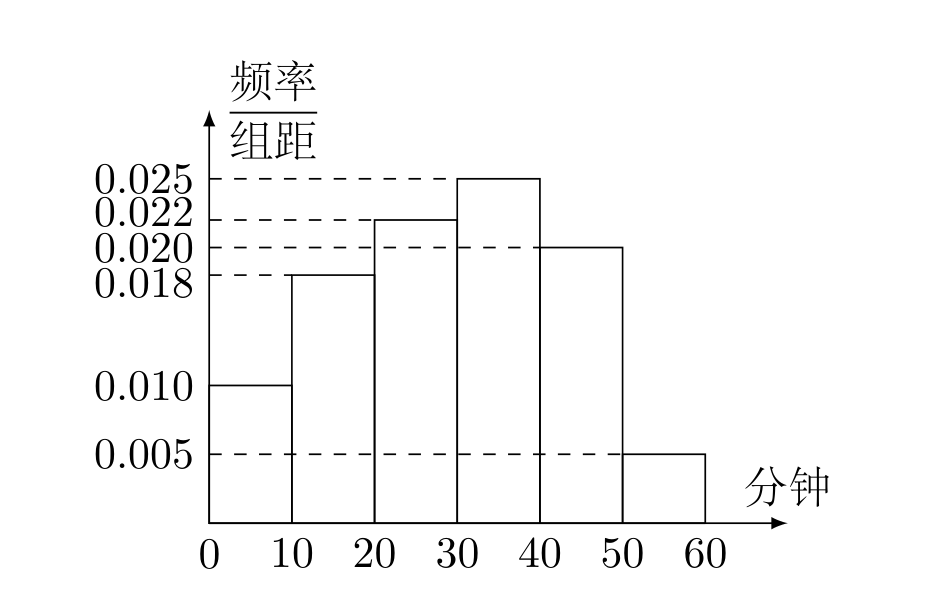
\includegraphics[width=0.42\linewidth]{GaoKao/images/2012/liaoning_science/q19_fig1.png}
\end{center}

        \item 如图，椭圆 \(C_{0}:\frac{x^{2}}{a^{2}} + \frac{y^{2}}{b^{2}} = 1\)（\(a > b > 0\)，\(\ a\)，\(b\) 为常数），动圆 \(C_1: x^2 + y^2 = t_1^2\)（\(b < t_1 < a\)）. 点 \(A_{1}\)，\(A_{2}\) 分别为 \(C_0\) 的左，右顶点，\(C_1\) 与 \(C_0\) 相交于 \(A\)，\(B\)，\(C\)，\(D\) 四点.

\begin{enumerate}
\item 求直线 \(AA_{1}\) 与直线 \(A_{2}B\) 交点 \(M\) 的轨迹方程.
\item 设动圆 \(C: x^{2} + y^{2} = t_{2}^{2}\) 与 \(C_{0}\) 相交于 \(A'\)，\(B'\)，\(C'\)，\(D'\) 四点，其中 \(b < t_{2} < a\)，\(t_{1} \neq t_{2}\). 若矩形 \(ABCD\) 与矩形 \(A'B'C'D'\) 的面积相等，证明：\(t_{1}^{2} + t_{2}^{2}\) 为定值.
\end{enumerate}

\begin{center}
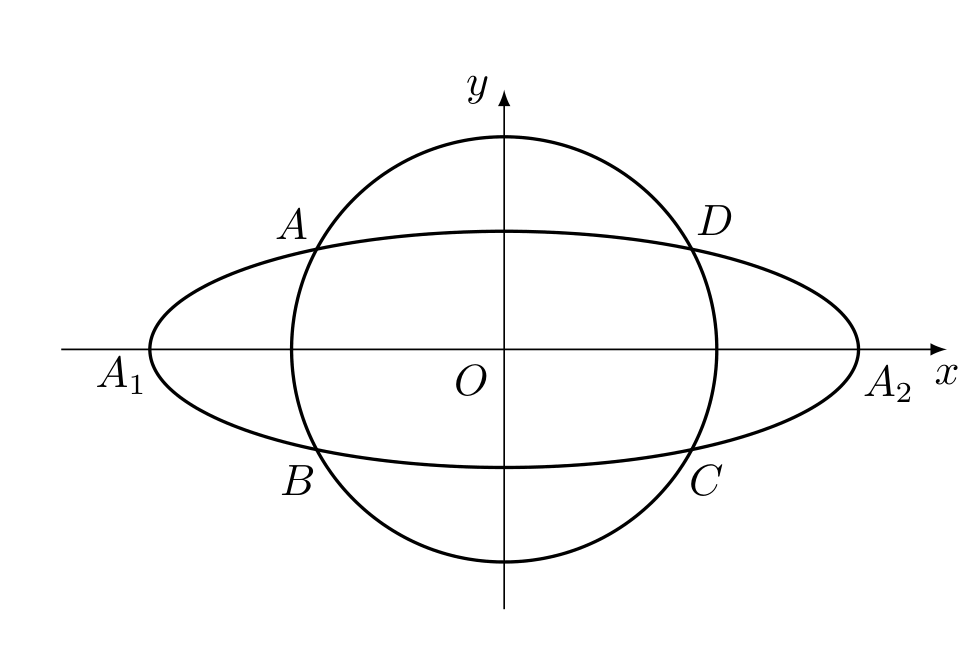
\includegraphics[width=8.0cm]{GaoKao/images/2012/liaoning_science/q20_fig1.png}
\end{center}

        \item 设 \(f(x) = \ln (x + 1) + \sqrt{x + 1} + ax + b\)（\(a\)，\(b \in \mathbb{R}\)，\(a\)，\(b\) 为常数），曲线 \(y = f(x)\) 与直线 \(y = \frac{3}{2} x\) 在 \((0,0)\) 点相切.

\begin{enumerate}
\item 求 \(a\)，\(b\) 的值.
\item 证明：当 \(0 < x < 2\) 时，\(f(x) < \frac{9x}{x + 6}\).
\end{enumerate}

    \end{enumerate}

\end{description}

\begin{description}

    \item[四、选考题]

    \begin{enumerate}[leftmargin=5pt]

      \addtocounter{enumi}{+21}

        \item \textbf{【选修4-1：几何证明选讲】}

如图，\(\odot O\) 和 \(\odot O'\) 相交于 \(A\)，\(B\) 两点，过 \(A\) 作两圆的切线分别交两圆于 \(C\)，\(D\) 两点，连接 \(DB\) 并延长交 \(\odot O'\) 于点 \(E\). 证明：

\begin{enumerate}
\item \(AC \cdot BD = AD \cdot AB\).
\item \(AC = AE\).
\end{enumerate}

\begin{center}
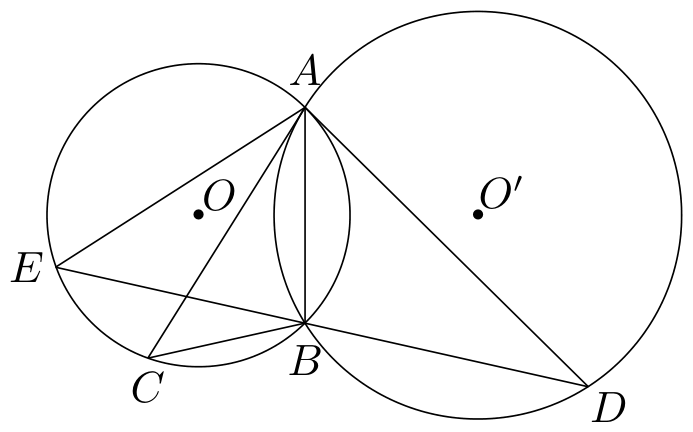
\includegraphics[width=8.1cm]{GaoKao/images/2012/liaoning_science/q22_fig1.png}
\end{center}

        \item \textbf{【选修4-4：坐标系与参数方程】}

在直角坐标系 \(xOy\) 中，圆 \(C_1: x^2 + y^2 = 4\)，圆 \(C_2: (x - 2)^2 + y^2 = 4\).

\begin{enumerate}
\item 在以 \(O\) 为极点，\(x\) 轴非负半轴为极轴的极坐标系中，分别写出圆 \(C_{1}\)，\(C_{2}\) 的极坐标方程，并求出圆 \(C_{1}\)，\(C_{2}\) 的交点坐标（用极坐标表示）.
\item 求圆 \(C_{1}\) 与 \(C_{2}\) 的公共弦的参数方程.
\end{enumerate}

        \item \textbf{【选修4-5：不等式选讲】}

已知 \(f(x) = |ax + 1|\)（\(a \in \mathbb{R}\)），不等式 \(f(x) \leqslant 3\) 的解集为 \(\{x \mid -2 \leqslant x \leqslant 1\}\).

\begin{enumerate}
\item 求 \(a\) 的值.
\item 若 \(\left|f(x)-2f\left(\frac{x}{2}\right)\right|\leqslant k\) 恒成立，求 \(k\) 的取值范围.
\end{enumerate}

    \end{enumerate}

\end{description}


\subsection{2012年辽宁卷（文）}\label{gk:2012年辽宁卷（文）}

\begin{description}

    \item[一、选择题]

    \begin{enumerate}[leftmargin=5pt]

        \item 已知向量 \(\bm{a} = (1, -1)\)，\(\bm{b} = (2, x)\). 若 \(\bm{a} \cdot \bm{b} = 1\)，则 \(x =\)（\quad）

        {\centering\begin{tabular*}{\linewidth}{@{}@{\extracolsep{\fill}}llll@{}}
          \text{A. }\(-1\)  &  \text{B. }\( -\frac{1}{2} \)  &  \text{C. }\( \frac{1}{2} \)  &  \text{D. }1
        \end{tabular*}\par}

        \item 已知全集 \(U = \{0, 1, 2, 3, 4, 5, 6, 7, 8, 9\}\)，集合 \(A = \{0, 1, 3, 5, 8\}\)，集合 \(B = \{2, 4, 5, 6, 8\}\)，则 \((\complement_U A) \cap (\complement_U B) =\)（\quad）

        {\centering\begin{tabular*}{\linewidth}{@{}@{\extracolsep{\fill}}llll@{}}
          \text{A. }\(\{5, 8\}\)  &  \text{B. }\(\{7, 9\}\)  &  \text{C. }\(\{0, 1, 3\}\)  &  \text{D. }\(\{2, 4, 6\}\)
        \end{tabular*}\par}

        \item 复数 \(\frac{1}{1 + \i} =\)（\quad）

        {\centering\begin{tabular*}{\linewidth}{@{}@{\extracolsep{\fill}}llll@{}}
          \text{A. }\(\frac{1}{2} - \frac{1}{2}\i\)  &  \text{B. }\(\frac{1}{2} + \frac{1}{2}\i\)  &  \text{C. }\(1 - \i\)  &  \text{D. }\(1 + \i\)
        \end{tabular*}\par}

        \item 在等差数列 \(\{a_{n}\}\) 中，已知 \(a_{4} + a_{8} = 16\)，则 \(a_{2} + a_{10} =\)（\quad）

        {\centering\begin{tabular*}{\linewidth}{@{}@{\extracolsep{\fill}}llll@{}}
          \text{A. }12  &  \text{B. }16  &  \text{C. }20  &  \text{D. }24
        \end{tabular*}\par}

        \item 已知命题 \(p: \forall x_1,x_2 \in \mathbb{R}\)，\((f(x_2) - f(x_1))(x_2 - x_1) \geqslant 0\)，则 \(\neg p\) 是（\quad）

        {\centering\begin{tabular*}{\linewidth}{@{}@{\extracolsep{\fill}}llll@{}}
          \text{A. }\(\exists x_{1},x_{2} \in \mathbb{R}\)，\((f(x_{2}) - f(x_{1}))(x_{2} - x_{1}) \leqslant 0\)  &  \text{B. }\(\forall x_{1},x_{2} \in \mathbb{R}\)，\((f(x_{2}) - f(x_{1}))(x_{2} - x_{1}) \leqslant 0\)  &  \text{C. }\(\exists x_{1},x_{2} \in \mathbb{R}\)，\((f(x_{2}) - f(x_{1}))(x_{2} - x_{1}) < 0\)  &  \text{D. }\(\forall x_{1},x_{2} \in \mathbb{R}\)，\((f(x_{2}) - f(x_{1}))(x_{2} - x_{1}) < 0\)
        \end{tabular*}\par}

        \item 已知 \(\sin \alpha - \cos \alpha = \sqrt{2}\)，\(\alpha \in (0, \pi)\)，则 \(\tan \alpha =\)（\quad）

        {\centering\begin{tabular*}{\linewidth}{@{}@{\extracolsep{\fill}}llll@{}}
          \text{A. }\(-1\)  &  \text{B. }\( -\frac{\sqrt{2}}{2} \)  &  \text{C. }\(\frac{\sqrt{2}}{2}\)  &  \text{D. }1
        \end{tabular*}\par}

        \item 将圆 \(x^{2} + y^{2} - 2x - 4y + 1 = 0\) 平分的直线是（\quad）

        {\centering\begin{tabular*}{\linewidth}{@{}@{\extracolsep{\fill}}llll@{}}
          \text{A. }\(x + y - 1 = 0\)  &  \text{B. }\(x + y + 3 = 0\)  &  \text{C. }\(x - y + 1 = 0\)  &  \text{D. }\(x - y + 3 = 0\)
        \end{tabular*}\par}

        \item 函数 \( y = \frac{1}{2} x^2 - \ln x \) 的单调递减区间为（\quad）

        {\centering\begin{tabular*}{\linewidth}{@{}@{\extracolsep{\fill}}llll@{}}
          \text{A. }\((-1, 1]\)  &  \text{B. }\((0,1]\)  &  \text{C. }\([1, +\infty)\)  &  \text{D. }\((0, +\infty)\)
        \end{tabular*}\par}

        \item 设变量 \(x\)，\(y\) 满足 \(\begin{cases}
x - y \leqslant 10,\\
0 \leqslant x + y \leqslant 20,\\
0 \leqslant y \leqslant 15,
\end{cases}\) 则 \(2x + 3y\) 的最大值为（\quad）

        {\centering\begin{tabular*}{\linewidth}{@{}@{\extracolsep{\fill}}llll@{}}
          \text{A. }20  &  \text{B. }35  &  \text{C. }45  &  \text{D. }55
        \end{tabular*}\par}

        \item 执行如图所示的程序框图，则输出的 \(S\) 值是（\quad）

\begin{center}
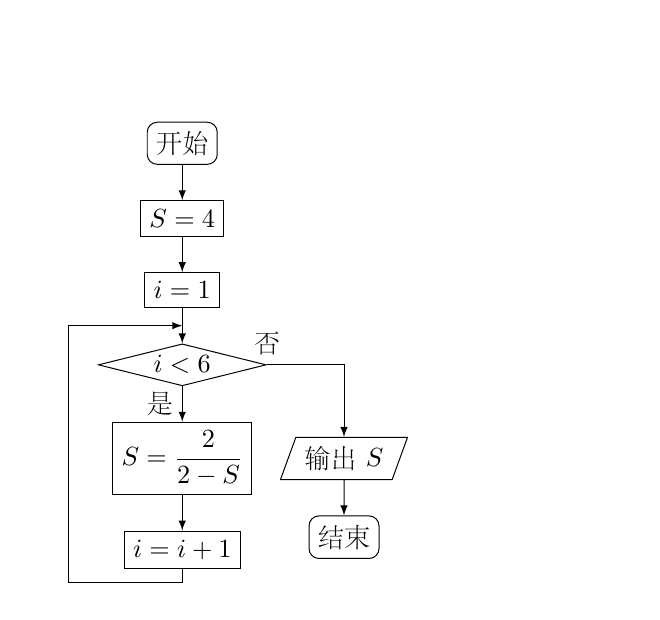
\includegraphics[width=0.78\linewidth]{GaoKao/images/2012/liaoning_liberal/q10_fig1.png}
\end{center}

        {\centering\begin{tabular*}{\linewidth}{@{}@{\extracolsep{\fill}}llll@{}}
          \text{A. }4  &  \text{B. }\( \frac{3}{2} \)  &  \text{C. }\( \frac{2}{3} \)  &  \text{D. }\(-1\)
        \end{tabular*}\par}

        \item 在长为 \(12 \mathrm{~cm}\) 的线段 \(AB\) 上任取一点 \(C\). 现作一矩形，邻边长分别等于线段 \(AC\)，\(CB\) 的长，则该矩形面积大于 \(20 \mathrm{~cm}^{2}\) 的概率为（\quad）

        {\centering\begin{tabular*}{\linewidth}{@{}@{\extracolsep{\fill}}llll@{}}
          \text{A. }\(\frac{1}{6}\)  &  \text{B. }\(\frac{1}{3}\)  &  \text{C. }\( \frac{2}{3} \)  &  \text{D. }\(\frac{4}{5}\)
        \end{tabular*}\par}

        \item 已知 \(P\)，\(Q\) 为抛物线 \(x^{2} = 2y\) 上两点，点 \(P\)，\(Q\) 的横坐标分别为 \(4\)，\(-2\). 过 \(P\)，\(Q\) 分别作抛物线的切线，两切线交于点 \(A\)，则点 \(A\) 的纵坐标为（\quad）

        {\centering\begin{tabular*}{\linewidth}{@{}@{\extracolsep{\fill}}llll@{}}
          \text{A. }1  &  \text{B. }3  &  \text{C. }\(-4\)  &  \text{D. }\(-8\)
        \end{tabular*}\par}

    \end{enumerate}

\end{description}

\begin{description}

    \item[二、填空题]

    \begin{enumerate}[leftmargin=5pt]

      \addtocounter{enumi}{+12}

        \item 一个几何体的三视图如图所示，则该几何体的体积为\rule[-0.3ex]{3em}{0.4pt}.

\begin{center}
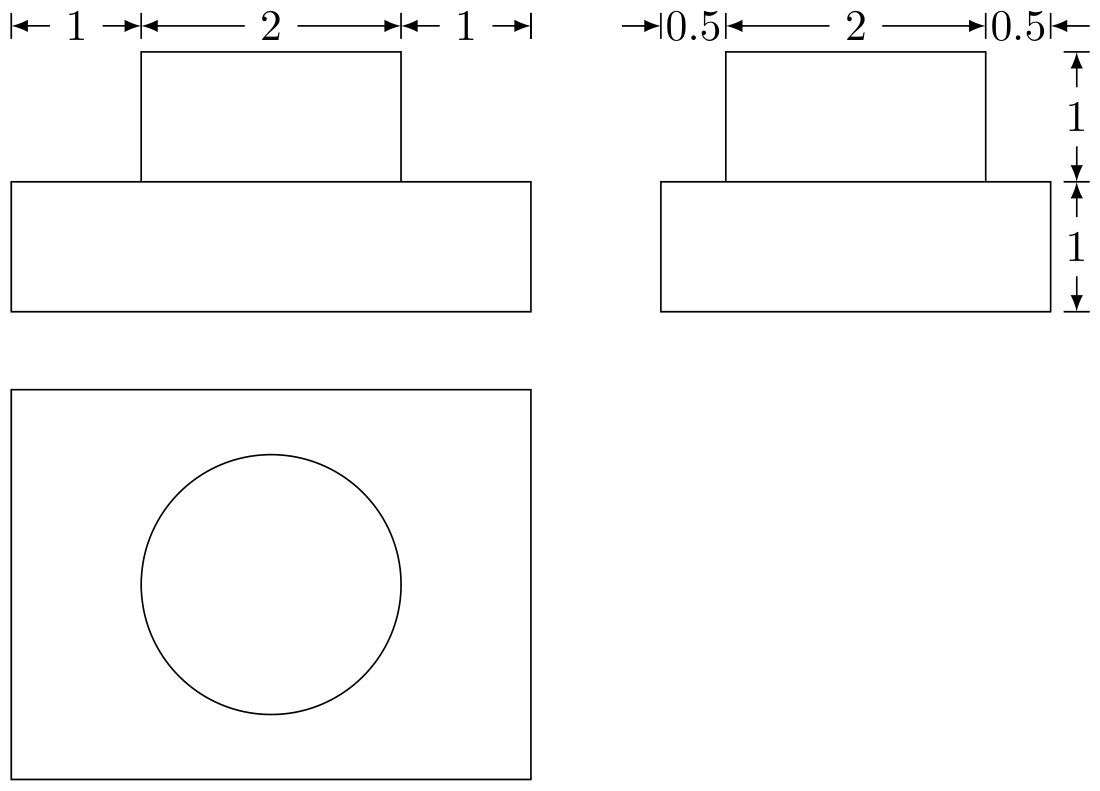
\includegraphics[width=11.0cm]{GaoKao/images/2012/liaoning_liberal/q13_fig1.png}
\end{center}

        \item 已知等比数列 \(\{a_{n}\}\) 为递增数列. 若 \(a_1 > 0\)，且 \(2(a_n + a_{n+2}) = 5a_{n+1}\)，则数列 \(\{a_n\}\) 的公比 \(q =\rule[-0.3ex]{3em}{0.4pt}\).

        \item 已知双曲线 \(x^{2} - y^{2} = 1\)，点 \(F_{1}\)，\(F_{2}\) 为其两个焦点，点 \(P\) 为双曲线上一点. 若 \(PF_{1} \perp PF_{2}\)，则 \(|PF_{1}| + |PF_{2}|\) 的值为\rule[-0.3ex]{3em}{0.4pt}.

        \item 已知点 \(P\)，\(A\)，\(B\)，\(C\)，\(D\) 是球 \(O\) 表面上的点，\(PA \perp\) 平面 \(ABCD\)，四边形 \(ABCD\) 是边长为 \(2\sqrt{3}\) 的正方形. 若 \(PA = 2\sqrt{6}\)，则 \(\triangle OAB\) 的面积为\rule[-0.3ex]{3em}{0.4pt}.

    \end{enumerate}

\end{description}

\begin{description}

    \item[三、解答题]

    \begin{enumerate}[leftmargin=5pt]

      \addtocounter{enumi}{+16}

        \item 在 \(\triangle ABC\) 中，角 \(A\)，\(B\)，\(C\) 的对边分别为 \(a\)，\(b\)，\(c\). 角 \(A\)，\(B\)，\(C\) 成等差数列.
\begin{enumerate}
\item 求 \(\cos B\) 的值；
\item 若边 \(a\)，\(b\)，\(c\) 成等比数列，求 \(\sin A \sin C\) 的值.
\end{enumerate}

        \item 如图，直三棱柱 \(ABC - A'B'C'\)，\(\angle BAC = 90^\circ\)，\(AB = AC = \sqrt{2}\)，\(AA' = 1\)，点 \(M\)，\(N\) 分别为 \(A'B\) 和 \(B'C'\) 的中点.
\begin{enumerate}
\item 证明： \(MN \parallel\) 平面 \(A'ACC'\)；
\item 求三棱锥 \( A' - MNC \) 的体积. （锥体体积公式 \( V = \frac{1}{3} Sh \)，其中 \(S\) 为底面积，\(h\) 为高）
\end{enumerate}

\begin{center}
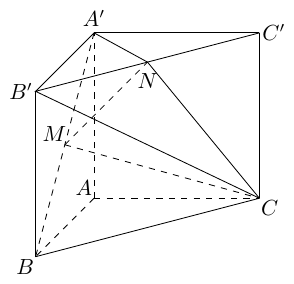
\includegraphics[width=6.8cm]{GaoKao/images/2012/liaoning_liberal/q18_fig1.png}
\end{center}

        \item 电视传媒公司为了解某地区观众对某类体育节目的收视情况，随机抽取了 \(100\text{ 名}\) 观众进行调查，其中女性有 \(55\text{ 名}\). 下面是根据调查结果绘制的观众日均收看该体育节目时间的频率分布直方图：

将日均收看该体育节目时间不低于 \(40\text{ 分钟}\) 的观众称为“体育迷”.

\begin{enumerate}
\item 根据已知条件完成下面的 \(2 \times 2\) 列联表，并据此资料你是否认为“体育迷”与性别有关？

\begin{center}
\begin{tabular}{|c|c|c|c|}
\hline
 & 非体育迷 & 体育迷 & 合计\\ \hline
男 & & & \\\hline
女 & & & \\\hline
合计 & & & \\\hline
\end{tabular}
\end{center}

\item 将日均收看该体育节目不低于 \(50\text{ 分钟}\) 的观众称为“超级体育迷”，已知“超级体育迷”中有 \(2\text{ 名}\) 女性. 若从“超级体育迷”中任意选取 \(2\text{ 人}\)，求至少有 \(1\text{ 名}\) 女性观众的概率.
\end{enumerate}

附：\(\chi^2 = \frac{n\left(n_{11}n_{22} - n_{12}n_{21}\right)^2}{n_{1+}n_{2+}n_{+1}n_{+2}}\).
\begin{center}
\begin{tabular}{c|cc}
\(P(\chi^2 \geqslant k)\) & \(0.05\) & \(0.01\) \\
\hline
\(k\) & \(3.841\) & \(6.635\)
\end{tabular}
\end{center}

\begin{center}
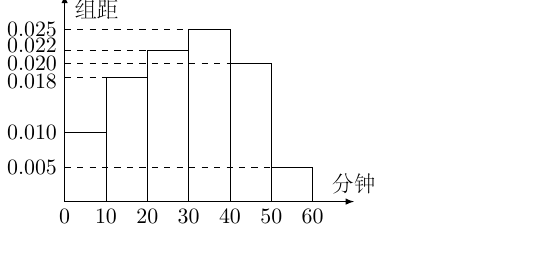
\includegraphics[width=0.6\linewidth]{GaoKao/images/2012/liaoning_liberal/q19_fig1.png}
\end{center}

        \item 如图，动圆 \(C_1: x^2 + y^2 = t^2\)，\(1 < t < 3\)，与椭圆 \(C_2: \frac{x^2}{9} + y^2 = 1\) 相交于 \(A\)，\(B\)，\(C\)，\(D\) 四点，点 \(A_1\)，\(A_2\) 分别为 \(C_2\) 的左，右顶点.
\begin{enumerate}
\item 当 \(t\) 为何值时，矩形 \(ABCD\) 的面积取得最大值？ 并求出其最大面积；
\item 求直线 \(AA_1\) 与直线 \(A_2B\) 交点 \(M\) 的轨迹方程.
\end{enumerate}

\begin{center}
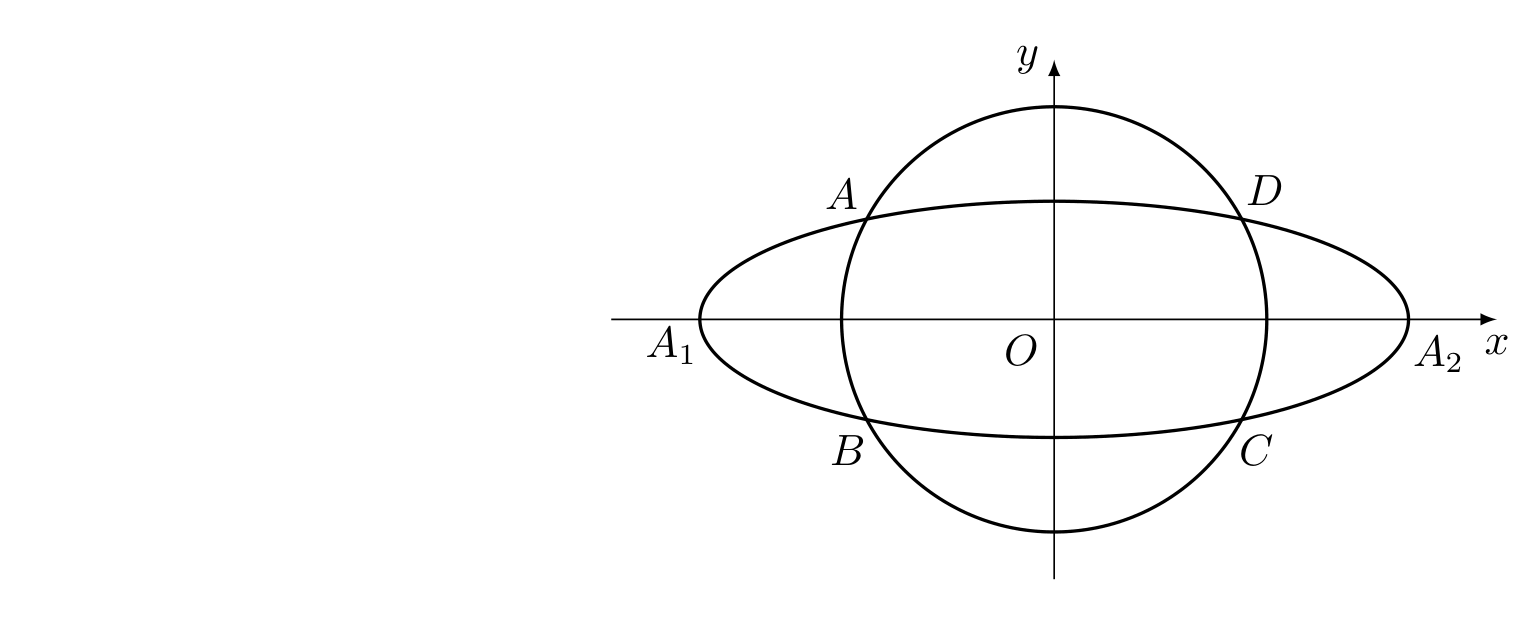
\includegraphics[width=11.0cm]{GaoKao/images/2012/liaoning_liberal/q20_fig1.png}
\end{center}

        \item 设 \( f(x) = \ln x + \sqrt{x} - 1\)，证明：
\begin{enumerate}
\item 当 \(x > 1\) 时，\(f(x) < \frac{3}{2}(x - 1)\)；
\item 当 \(1 < x < 3\) 时，\(f(x) < \frac{9(x - 1)}{x + 5}\).
\end{enumerate}

    \end{enumerate}

\end{description}

\begin{description}

    \item[四、选考题]

    \begin{enumerate}[leftmargin=5pt]

      \addtocounter{enumi}{+21}

        \item \textbf{【选修4-1：几何证明选讲】}

如图，\(\odot O\) 和 \(\odot O'\) 相交于 \(A\)，\(B\) 两点，过 \(A\) 作两圆的切线分别交两圆于 \(C\)，\(D\) 两点，连接 \(DB\) 并延长交 \(\odot O\) 于点 \(E\). 证明：
\begin{enumerate}
\item \(AC \cdot BD = AD \cdot AB\)；
\item \(AC = AE\).
\end{enumerate}

\begin{center}
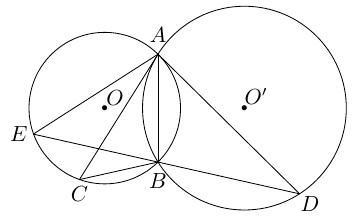
\includegraphics[width=7.8cm]{GaoKao/images/2012/liaoning_liberal/q22_fig1_rgb.png}
\end{center}

        \item \textbf{【选修4-4：坐标系与参数方程】}

在直角坐标系 \(xOy\) 中，圆 \(C_1: x^2 + y^2 = 4\)，圆 \(C_2: (x - 2)^2 + y^2 = 4\).
\begin{enumerate}
\item 在以 \(O\) 为极点，\(x\) 轴非负半轴为极轴的极坐标系中，分别写出圆 \(C_1\)，\(C_2\) 的极坐标方程，并求出圆 \(C_1\)，\(C_2\) 的交点坐标 （用极坐标表示）；
\item 求圆 \(C_1\) 与 \(C_2\) 的公共弦的参数方程.
\end{enumerate}

        \item \textbf{【选修4-5：不等式选讲】}

已知 \( f(x) = |ax + 1| \)（\(a \in \mathbb{R}\)），不等式 \( f(x) \leqslant 3 \) 的解集为 \(\{x \mid -2 \leqslant x \leqslant 1\}\).
\begin{enumerate}
\item 求 \(a\) 的值；
\item 若 \(\left|f(x)-2f\left(\frac{x}{2}\right)\right|\leqslant k\) 恒成立，求 \(k\) 的取值范围.
\end{enumerate}

    \end{enumerate}

\end{description}


\subsection{2012年上海卷（理）}\label{gk:2012年上海卷（理）}

\begin{description}

    \item[一、填空题]

    \begin{enumerate}[leftmargin=5pt]

        \item 计算： \( \frac{3-\i}{1+\i}= \)\rule[-0.3ex]{3em}{0.4pt}（\(\i\) 为虚数单位）.

        \item 若集合 \(A = \{x \mid 2x + 1 > 0\}\)，\(B = \{x \mid |x - 1| < 2\}\)，则 \(A \cap B = \)\rule[-0.3ex]{3em}{0.4pt}.

        \item 函数 \( f(x) = \left| \begin{matrix} 2 & \cos x \\ \sin x & -1 \end{matrix} \right| \) 的值域是\rule[-0.3ex]{3em}{0.4pt}.

        \item 若 \(\bm{n} = (-2,1)\) 是直线 \(l\) 的一个法向量，则 \(l\) 的倾斜角的大小为\rule[-0.3ex]{3em}{0.4pt}. （结果用反三角函数值表示）

        \item 在 \(\left(x - \frac{2}{x}\right)^6\) 的二项展开式中，常数项等于\rule[-0.3ex]{3em}{0.4pt}.

        \item 有一列正方体，棱长组成以 1 为首项，\(\frac{1}{2}\) 为公比的等比数列，体积分别记为 \(V_{1}\)，\(V_{2}\)，\(\cdots\)，\(V_{n}\)，\(\cdots\)，则 \(\displaystyle\lim_{n \to \infty} (V_{1} + V_{2} + \cdots + V_{n}) =\rule[-0.3ex]{3em}{0.4pt}.\)

        \item 已知函数 \( f(x) = {\mathrm{e}}^{|x - a|} \) （\( a \) 为常数）. 若 \( f(x) \) 在区间 \([1, +\infty)\) 上是增函数，则 \( a \) 的取值范围是\rule[-0.3ex]{3em}{0.4pt}.

        \item 若一个圆锥的侧面展开图是面积为 \(2\pi\) 的半圆面，则该圆锥的体积为\rule[-0.3ex]{3em}{0.4pt}.

        \item 已知 \( y = f(x) + x^2 \) 是奇函数，且 \( f(1) = 1 \). 若 \( g(x) = f(x) + 2 \)，则 \( g(-1) = \)\rule[-0.3ex]{3em}{0.4pt}.

        \item 如图，在极坐标系中，过点 \(M(2,0)\) 的直线 \(l\) 与极轴的夹角 \(\alpha = \frac{\pi}{6}\). 若将 \(l\) 的极坐标方程写成 \(\rho = f(\theta)\) 的形式，则 \(f(\theta) =\rule[-0.3ex]{3em}{0.4pt}.\)
\begin{center}
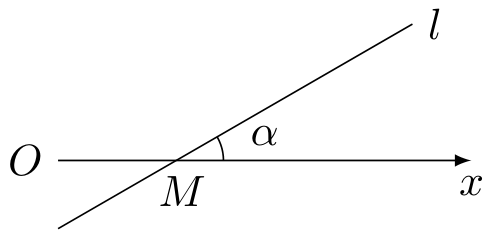
\includegraphics[width=5.7cm]{GaoKao/images/2012/shanghai_science/q10_fig1.png}
\end{center}

        \item 三位同学参加跳高，跳远，铅球项目的比赛. 若每人都选择其中两个项目，则有且仅有两人选择的项目完全相同的概率是\rule[-0.3ex]{3em}{0.4pt}. （结果用最简分数表示）

        \item 在平行四边形 \(ABCD\) 中，\(\angle A = \frac{\pi}{3}\)，边 \(AB\)，\(AD\) 的长分别为 \(2\)，\(1\). 若 \(M\)，\(N\) 分别是边 \(BC\)，\(CD\) 上的点，且满足 \(\frac{|BM|}{|BC|} = \frac{|CN|}{|CD|}\)，则 \(\overrightarrow{AM} \cdot \overrightarrow{AN}\) 的取值范围是\rule[-0.3ex]{3em}{0.4pt}.

        \item 已知函数 \( y = f(x) \) 的图象是折线段 \(ABC\)，其中 \( A(0,0) \)，\( B\left(\frac{1}{2}, 5\right) \)，\( C(1,0) \). 函数 \( y = xf(x) \)（\(0 \leqslant x \leqslant 1\)）的图象与 \( x \) 轴围成的图形的面积为\rule[-0.3ex]{3em}{0.4pt}.

        \item 如图，\(AD\) 与 \(BC\) 是四面体 \(ABCD\) 中互相垂直的棱，\(BC = 2\). 若 \(AD = 2c\)，且 \(AB + BD = AC + CD = 2a\)，其中 \(a\)，\(c\) 为常数，则四面体 \(ABCD\) 的体积的最大值是\rule[-0.3ex]{3em}{0.4pt}.
\begin{center}
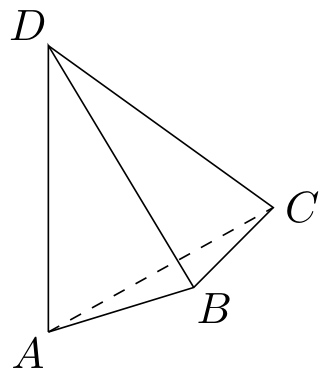
\includegraphics[width=4.1cm]{GaoKao/images/2012/shanghai_science/q14_fig1.png}
\end{center}

    \end{enumerate}

\end{description}

\begin{description}

    \item[二、选择题]

    \begin{enumerate}[leftmargin=5pt]

      \addtocounter{enumi}{+14}

        \item 若 \(1 + \sqrt{2}i\) 是关于 \(x\) 的实系数方程 \(x^{2} + bx + c = 0\) 的一个复数根，则（\quad）

        {\centering\begin{tabular*}{\linewidth}{@{}@{\extracolsep{\fill}}llll@{}}
          \text{A. }\(b = 2\)，\(c = 3\)  &  \text{B. }\(b = -2\)，\(c = 3\)  &  \text{C. }\(b = -2\)，\(c = -1\)  &  \text{D. }\(b = 2\)，\(c = -1\)
        \end{tabular*}\par}

        \item 在 \(\triangle ABC\) 中，若 \(\sin^2 A + \sin^2 B < \sin^2 C\)，则 \(\triangle ABC\) 的形状是（\quad）

        {\centering\begin{tabular*}{\linewidth}{@{}@{\extracolsep{\fill}}llll@{}}
          \text{A. }锐角三角形  &  \text{B. }直角三角形  &  \text{C. }钝角三角形  &  \text{D. }不能确定
        \end{tabular*}\par}

        \item 设 \(10 \leqslant x_{1} < x_{2} < x_{3} < x_{4} \leqslant 10^{4}\)，\(x_{5} = 10^{5}\). 随机变量 \(\xi_{1}\) 取值 \(x_{1}\)，\(x_{2}\)，\(x_{3}\)，\(x_{4}\)，\(x_{5}\) 的概率均为 0.2. 随机变量 \(\xi_{2}\) 取值 \(\frac{x_{1} + x_{2}}{2}\)，\(\frac{x_{2} + x_{3}}{2}\)，\(\frac{x_{3} + x_{4}}{2}\)，\(\frac{x_{4} + x_{5}}{2}\)，\(\frac{x_{5} + x_{1}}{2}\) 的概率也均为 0.2. 若记 \(D(\xi_{1})\)，\(D(\xi_{2})\) 分别为 \(\xi_{1}\)，\(\xi_{2}\) 的方差，则（\quad）

        {\centering\begin{tabular*}{\linewidth}{@{}@{\extracolsep{\fill}}llll@{}}
          \text{A. }\(D(\xi_{1}) > D(\xi_{2})\)  &  \text{B. }\(D(\xi_{1}) = D(\xi_{2})\)  &  \text{C. }\(D(\xi_{1}) < D(\xi_{2})\)  &  \text{D. }\(D(\xi_{1})\) 与 \(D(\xi_{2})\) 的大小关系与 \(x_{1}\)，\(x_{2}\)，\(x_{3}\)，\(x_{4}\) 的取值有关
        \end{tabular*}\par}

        \item 设 \(a_{n} = \frac{1}{n}\sin \frac{n\pi}{25}\)，\(S_{n} = a_{1} + a_{2} + \cdots + a_{n}\). 在 \(S_{1}\)，\(S_{2}\)，\(\cdots\)，\(S_{100}\) 中，正数的个数是（\quad）

        {\centering\begin{tabular*}{\linewidth}{@{}@{\extracolsep{\fill}}llll@{}}
          \text{A. }25  &  \text{B. }50  &  \text{C. }75  &  \text{D. }100
        \end{tabular*}\par}

    \end{enumerate}

\end{description}

\begin{description}

    \item[三、解答题]

    \begin{enumerate}[leftmargin=5pt]

      \addtocounter{enumi}{+18}

        \item 如图，在四棱锥 \(P - ABCD\) 中，底面 \(ABCD\) 是矩形，\(PA \perp\) 底面 \(ABCD\)，\(E\) 是 \(PC\) 的中点. 已知 \(AB = 2\)，\(AD = 2\sqrt{2}\)，\(PA = 2\). 求：

\begin{enumerate}
\item 三角形 \(PCD\) 的面积；
\item 异面直线 \(BC\) 与 \(AE\) 所成角的大小.
\end{enumerate}

\begin{center}
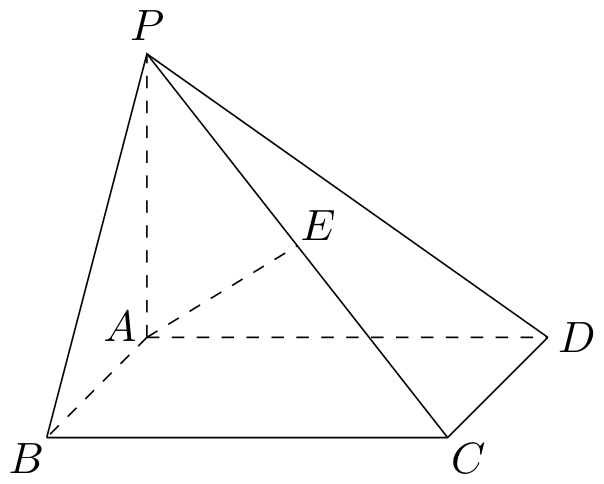
\includegraphics[width=7.5cm]{GaoKao/images/2012/shanghai_science/q19_fig1.png}
\end{center}

        \item 已知函数 \( f(x) = \lg (x + 1) \).

\begin{enumerate}
\item 若 \(0 < f(1 - 2x) + f(x) < 1\)，求 \(x\) 的取值范围；
\item 若 \(g(x)\) 是以 2 为周期的偶函数，且当 \(0 \leqslant x \leqslant 1\) 时，有 \(g(x) = f(x)\)，求函数 \(y = g(x)\) （\(x \in [1, 2]\)） 的反函数.
\end{enumerate}

        \item 海事救援船对一艘失事船进行定位：以失事船的当前位置为原点，以正北方向为 \(y\) 轴正方向建立平面直角坐标系（以 \(1\text{ 海里}\) 为单位长度），则救援船恰好在失事船正南方向 \(12\text{ 海里}\) \(A\) 处，如图. 现假设：

\begin{enumerate}
\item 失事船的移动路径可视为抛物线 \(y = \frac{12}{49} x^2\)；
\item 定位后救援船即刻沿直线匀速前往救援；
\item 救援船出发 \(t\) 小时后，失事船所在位置的横坐标为 \(7t\).
\end{enumerate}

\begin{enumerate}
\item 当 \(t = 0.5\) 时，写出失事船所在位置 \(P\) 的纵坐标. 若此时两船恰好会合，求救援船速度的大小和方向；
\item 问救援船的时速至少是多少海里才能追上失事船？
\end{enumerate}

\begin{center}
\includegraphics[width=7.2cm]{GaoKao/images/2012/shanghai_science/q21_fig1.png}
\end{center}

        \item 在平面直角坐标系 \(xOy\) 中，已知双曲线 \(C_1: 2x^2 - y^2 = 1\).

\begin{enumerate}
\item 过 \(C_{1}\) 的左顶点引 \(C_{1}\) 的一条渐近线的平行线，求该直线与另一条渐近线及 \(x\) 轴围成的三角形的面积；
\item 设斜率为 1 的直线 \(l\) 交 \(C_{1}\) 于 \(P\)，\(Q\) 两点. 若 \(l\) 与圆 \(x^{2} + y^{2} = 1\) 相切. 求证： \(OP \perp OQ\)；
\item 设椭圆 \(C_{2}: 4x^{2} + y^{2} = 1\). 若 \(M\)，\(N\) 分别是 \(C_{1}\)，\(C_{2}\) 上的动点，且 \(OM \perp ON\)，求证：\(O\) 到直线 \(MN\) 的距离是定值.
\end{enumerate}

        \item 对于数集 \(X = \{-1, x_1, x_2, \cdots, x_n\}\)，其中 \(0 < x_1 < x_2 < \cdots < x_n\)，\(n \geqslant 2\)，定义向量集 \(Y = \{\bm{a} \mid \bm{a} = (s, t), s \in X, t \in X\}\). 若对任意 \(\bm{a}_1 \in Y\)，存在 \(\bm{a}_2 \in Y\)，使得 \(\bm{a}_1 \cdot \bm{a}_2 = 0\)，则称 \(X\) 具有性质 \(P\). 例如 \(\{-1, 1, 2\}\) 具有性质 \(P\).

\begin{enumerate}
\item 若 \(x > 2\)，且 \(\{-1, 1, 2, x\}\) 具有性质 \(P\)，求 \(x\) 的值；
\item 若 \(X\) 具有性质 \(P\)，求证： \(1 \in X\)，且当 \(x_n > 1\) 时，\(x_1 = 1\)；
\item 若 \(X\) 具有性质 \(P\)，且 \(x_{1} = 1\)，\(x_{2} = q\) （\(q\) 为常数），求有穷数列 \(x_{1}\)，\(x_{2}\)，\(\cdots\)，\(x_{n}\) 的通项公式.
\end{enumerate}

    \end{enumerate}

\end{description}


\subsection{2012年上海卷（文）}\label{gk:2012年上海卷（文）}

\begin{description}

    \item[一、填空题]

    \begin{enumerate}[leftmargin=5pt]

        \item 计算： \(\frac{3 - \i}{1 + \i} =\)\rule[-0.3ex]{3em}{0.4pt}.（\(\i\) 为虚数单位）

        \item 若集合 \(A = \{x \mid 2x - 1 > 0\}\)，\(B = \{x \mid |x| < 1\}\)，则 \(A \cap B =\)\rule[-0.3ex]{3em}{0.4pt}.

        \item 函数 \( f(x) = \left| \begin{matrix} \sin x & 2 \\ -1 & \cos x \end{matrix} \right| \) 的最小正周期是\rule[-0.3ex]{3em}{0.4pt}.

        \item 若 \(\bm{d} = (2,1)\) 是直线 \(l\) 的一个方向向量，则 \(l\) 的倾斜角的大小为\rule[-0.3ex]{3em}{0.4pt}. （结果用反三角函数值表示）

        \item 一个高为 \(2\) 的圆柱，底面周长为 \(2\pi\). 该圆柱的表面积为\rule[-0.3ex]{3em}{0.4pt}.

        \item 方程 \(4^{x} - 2^{x + 1} - 3 = 0\) 的解是\rule[-0.3ex]{3em}{0.4pt}.

        \item 有一列正方体，棱长组成以 1 为首项，\(\frac{1}{2}\) 为公比的等比数列，体积分别记为 \(V_{1}\)，\(V_{2}\)，\(\cdots\)，\(V_{n}\)，\(\cdots\)，则 \(\lim\limits_{n \to \infty} (V_{1} + V_{2} + \cdots + V_{n}) =\)\rule[-0.3ex]{3em}{0.4pt}.

        \item 在 \(\left(x - \frac{1}{x}\right)^{6}\) 的二项展开式中，常数项等于\rule[-0.3ex]{3em}{0.4pt}.

        \item 已知 \( y = f(x) \) 是奇函数，若 \( g(x) = f(x) + 2 \) 且 \( g(1) = 1 \)，则 \( g(-1) = \)\rule[-0.3ex]{3em}{0.4pt}.

        \item 满足约束条件 \( |x| + 2|y| \leqslant 2 \) 的目标函数 \( z = y - x \) 的最小值是\rule[-0.3ex]{3em}{0.4pt}.

        \item 三位同学参加跳高，跳远，铅球项目的比赛. 若每人只选择一个项目，则有且仅有两人选择的项目相同的概率是\rule[-0.3ex]{3em}{0.4pt}. （结果用最简分数表示）

        \item 在矩形 \(ABCD\) 中，边 \(AB\)、\(AD\) 的长分别为 \(2\)、\(1\). 若 \(M\)、\(N\) 分别是 \(BC\)、\(CD\) 上的点，且满足 \(\frac{|BM|}{|BC|} = \frac{|CN|}{|CD|}\)，则 \(\overrightarrow{AM} \cdot \overrightarrow{AN}\) 的取值范围是\rule[-0.3ex]{3em}{0.4pt}.

        \item 已知函数 \( y = f(x) \) 的图象是折线段 \(ABC\)，其中 \(A(0,0)\)，\(B\left(\frac{1}{2}, 1\right)\)，\(C(1,0)\). 函数 \(y = xf(x)\) （\(0 \leqslant x \leqslant 1\)） 的图象与 \(x\) 轴围成的图形的面积为\rule[-0.3ex]{3em}{0.4pt}.

        \item 已知 \( f(x) = \frac{1}{1 + x} \)，各项均为正数的数列 \(\{a_n\}\) 满足 \(a_{1} = 1\)，\(a_{n + 2} = f(a_n)\). 若 \( a_{2010} = a_{2012} \)，则 \( a_{20} + a_{11} \) 的值是\rule[-0.3ex]{3em}{0.4pt}.

    \end{enumerate}

\end{description}

\begin{description}

    \item[二、选择题]

    \begin{enumerate}[leftmargin=5pt]

      \addtocounter{enumi}{+14}

        \item 若 \(1 + \sqrt{2}\i\) 是关于 \(x\) 的实系数方程 \(x^{2} + bx + c = 0\) 的一个复数根，则（\quad）

        {\centering\begin{tabular*}{\linewidth}{@{}@{\extracolsep{\fill}}llll@{}}
          \text{A. }\(b = 2, c = 3\)  &  \text{B. }\(b = 2\)，\(c = -1\)  &  \text{C. }\(b = -2\)，\(c = -1\)  &  \text{D. }\(b = -2\)，\(c = 3\)
        \end{tabular*}\par}

        \item 对于常数 \(m\)，\(n\)，“\(mn > 0\)”是“方程 \(mx^{2} + ny^{2} = 1\) 表示的曲线是椭圆”的（\quad）

        {\centering\begin{tabular*}{\linewidth}{@{}@{\extracolsep{\fill}}llll@{}}
          \text{A. }充分不必要条件  &  \text{B. }必要不充分条件  &  \text{C. }充分必要条件  &  \text{D. }既不充分也不必要条件
        \end{tabular*}\par}

        \item 在 \(\triangle ABC\) 中，若 \(\sin^{2} A + \sin^{2} B < \sin^{2} C\)，则 \(\triangle ABC\) 的形状是（\quad）

        {\centering\begin{tabular*}{\linewidth}{@{}@{\extracolsep{\fill}}llll@{}}
          \text{A. }钝角三角形  &  \text{B. }直角三角形  &  \text{C. }锐角三角形  &  \text{D. }不能确定
        \end{tabular*}\par}

        \item 若 \(S_{n} = \sin \frac{\pi}{7} + \sin \frac{2\pi}{7} + \cdots + \sin \frac{n\pi}{7}\) （\(n \in \mathbb{N}^{*}\)），则在 \(S_{1}\)，\(S_{2}\)，\(\cdots\)，\(S_{100}\) 中，正数的个数是（\quad）

        {\centering\begin{tabular*}{\linewidth}{@{}@{\extracolsep{\fill}}llll@{}}
          \text{A. }16  &  \text{B. }72  &  \text{C. }86  &  \text{D. }100
        \end{tabular*}\par}

    \end{enumerate}

\end{description}

\begin{description}

    \item[三、解答题]

    \begin{enumerate}[leftmargin=5pt]

      \addtocounter{enumi}{+18}

        \item 如图，在三棱锥 \(P - ABC\) 中，\(PA \perp\) 底面 \(ABC\)，\(D\) 是 \(PC\) 的中点. 已知 \(\angle BAC = \frac{\pi}{2}\)，\(AB = 2\)，\(AC = 2\sqrt{3}\)，\(PA = 2\). 求：
\begin{enumerate}
\item 三棱锥 \(P - ABC\) 的体积；
\item 异面直线 \(BC\) 与 \(AD\) 所成的角的大小（结果用反三角函数值表示）.
\end{enumerate}

\begin{center}
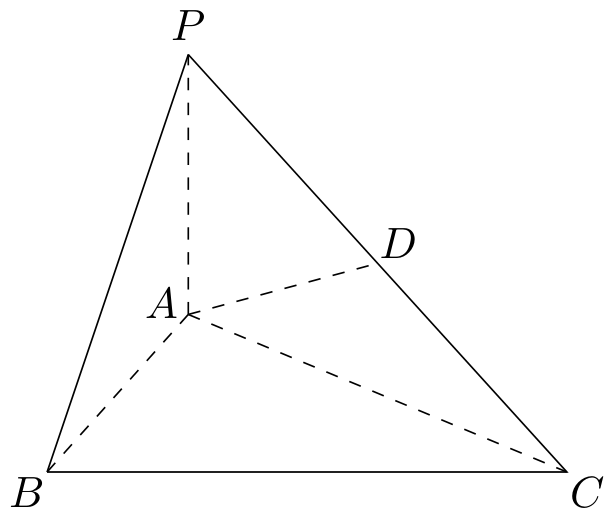
\includegraphics[width=7.6cm]{GaoKao/images/2012/shanghai_liberal/q19_fig1.png}
\end{center}

        \item 已知函数 \(f(x) = \lg (x + 1)\).
\begin{enumerate}
\item 若 \(0 < f(1 - 2x) - f(x) < 1\)，求 \(x\) 的取值范围；
\item 若 \(g(x)\) 是以 2 为周期的偶函数，且当 \(0 \leqslant x \leqslant 1\) 时，有 \(g(x) = f(x)\)，求函数 \(y = g(x)\) （\(x \in [1,2]\)） 的反函数.
\end{enumerate}

        \item 海事救援船对一艘失事船进行定位：以失事船的当前位置为原点，以正北方向为 \(y\) 轴正方向建立平面直角坐标系（以 1 海里为单位长度），则救援船恰好在失事船正南方向 12 海里 \(A\) 处，如图. 现假设：
\begin{enumerate}
\item 失事船的移动路径可视为抛物线 \(y = \frac{12}{49} x^{2}\)；
\item 定位后救援船即刻沿直线匀速前往救援；
\item 救援船出发 \(t\) 小时后，失事船所在位置的横坐标为 \(7t\).
\end{enumerate}
\begin{enumerate}
\item 当 \(t = 0.5\) 时，写出失事船所在位置 \(P\) 的纵坐标. 若此时两船恰好会合，求救援船速度的大小和方向；
\item 问救援船的时速至少是多少海里才能追上失事船？
\end{enumerate}

\begin{center}
\includegraphics[width=7.2cm]{GaoKao/images/2012/shanghai_liberal/q21_fig1.png}
\end{center}

        \item 在平面直角坐标系 \(xOy\) 中，已知双曲线 \(C: 2x^{2} - y^{2} = 1\).
\begin{enumerate}
\item 设 \(F\) 是 \(C\) 的左焦点，点 \(M\) 是 \(C\) 右支上一点. 若 \(|MF| = 2\sqrt{2}\)，求点 \(M\) 的坐标；
\item 过 \(C\) 的左顶点作 \(C\) 的两条渐近线的平行线. 求这两组平行线围成的平行四边形的面积；
\item 设斜率为 \(k\) （\(|k| < \sqrt{2}\)） 的直线 \(l\) 交 \(C\) 于 \(P\)，\(Q\) 两点. 若 \(l\) 与圆 \(x^{2} + y^{2} = 1\) 相切，求证： \(OP \perp OQ\).
\end{enumerate}

        \item 对于项数为 \(m\) 的有穷数列 \(\{a_{n}\}\)，记 \(b_{k} = \max \{a_{1}, a_{2}, \cdots, a_{k}\}\) （\(k = 1, 2, \cdots, m\)），即 \(b_{k}\) 为 \(a_{1}\)，\(a_{2}\)，\(\cdots\)，\(a_{k}\) 中的最大值，并称数列 \(\{b_{k}\}\) 是 \(\{a_{n}\}\) 的控制数列. 如 1， 3， 2， 5， 5 的控制数列是 1， 3， 3， 5， 5.
\begin{enumerate}
\item 若各项均为正整数的数列 \(\{a_{n}\}\) 的控制数列为 2， 3， 4， 5， 5，写出所有的 \(\{a_{n}\}\)；
\item 设 \(\{b_{n}\}\) 是 \(\{a_{n}\}\) 的控制数列，满足 \(a_{k} + b_{m - k + 1} = C\) （\(C\) 为常数，\(k = 1\)，\(2\)，\(\cdots\)，\(m\)）. 求证：\(b_{k} = a_{k}\) （\(k = 1, 2, \cdots, m\)）；
\item 设 \(m = 100\)，常数 \(a \in \left(\frac{1}{2}, 1\right)\)，若 \(a_{n} = a n^{2} - (-1)^{\frac{n(n + 1)}{2}} n\)，\(\{b_{n}\}\) 是 \(\{a_{n}\}\) 的控制数列，求 \((b_{1} - a_{1}) + (b_{2} - a_{2}) + \cdots + (b_{100} - a_{100})\).
\end{enumerate}

    \end{enumerate}

\end{description}


\subsection{2012年四川卷（理）}\label{gk:2012年四川卷（理）}

\begin{description}

    \item[一、选择题]

    \begin{enumerate}[leftmargin=5pt]

        \item \((1 + x)^{7}\) 的展开式中 \(x^{2}\) 的系数是（\quad）

        {\centering\begin{tabular*}{\linewidth}{@{}@{\extracolsep{\fill}}llll@{}}
          \text{A. }42  &  \text{B. }35  &  \text{C. }28  &  \text{D. }21
        \end{tabular*}\par}

        \item 复数 \(\frac{(1 - \i)^2}{2\i} =\)（\quad）

        {\centering\begin{tabular*}{\linewidth}{@{}@{\extracolsep{\fill}}llll@{}}
          \text{A. }1  &  \text{B. }\(-1\)  &  \text{C. }\(\i\)  &  \text{D. }\(-\i\)
        \end{tabular*}\par}

        \item 函数 \( f(x) = \begin{cases}
\frac{x^2 - 9}{x - 3}, & x < 3,\\
\ln (x - 2), & x \geqslant 3,
\end{cases} \) 在 \( x = 3 \) 处的极限是（\quad）

        {\centering\begin{tabular*}{\linewidth}{@{}@{\extracolsep{\fill}}llll@{}}
          \text{A. }不存在  &  \text{B. }等于 6  &  \text{C. }等于 3  &  \text{D. }等于 0
        \end{tabular*}\par}

        \item 如图，正方形 \(ABCD\) 的边长为 \(1\)，延长 \(BA\) 至 \(E\)，使 \(AE=1\)，连接 \(EC\)，\(ED\)，则 \(\sin \angle CED =\)（\quad）

\begin{center}
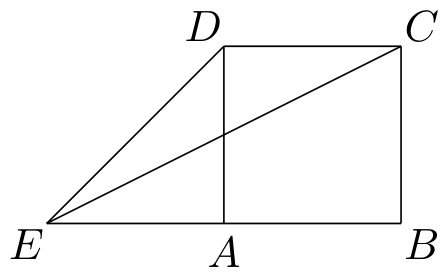
\includegraphics[width=5.6cm]{GaoKao/images/2012/sichuan_science/q4_fig1.png}
\end{center}

        {\centering\begin{tabular*}{\linewidth}{@{}@{\extracolsep{\fill}}llll@{}}
          \text{A. }\(\frac{3\sqrt{10}}{10}\)  &  \text{B. }\(\frac{\sqrt{10}}{10}\)  &  \text{C. }\(\frac{\sqrt{5}}{10}\)  &  \text{D. }\(\frac{\sqrt{5}}{15}\)
        \end{tabular*}\par}

        \item 函数 \( y = a^x - \frac{1}{a} \)（\(a > 0, a \neq 1\)）的图象可能是（\quad）

        {\centering\begin{tabular*}{\linewidth}{@{}@{\extracolsep{\fill}}cccc@{}}
          \text{A. }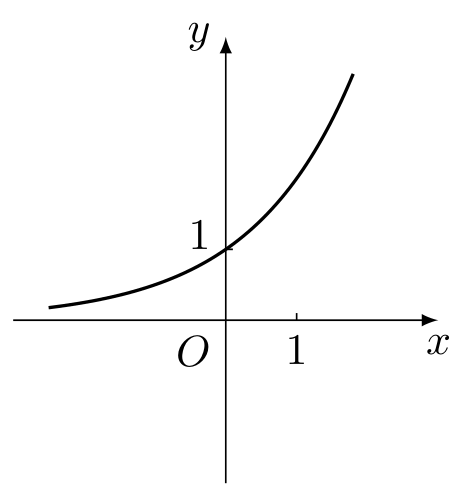
\includegraphics[width=0.15\paperwidth]{GaoKao/images/2012/sichuan_science/q5_choice_a.png}  &  \text{B. }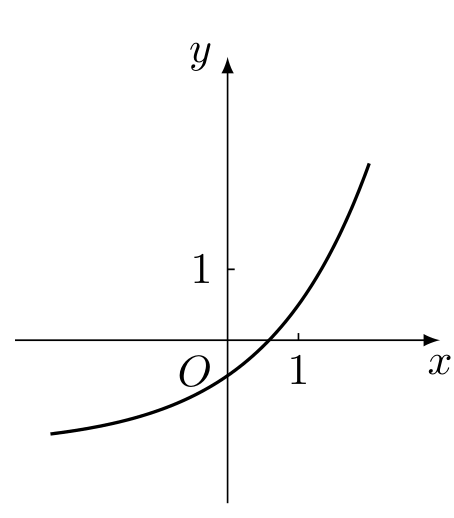
\includegraphics[width=0.15\paperwidth]{GaoKao/images/2012/sichuan_science/q5_choice_b.png}  &  \text{C. }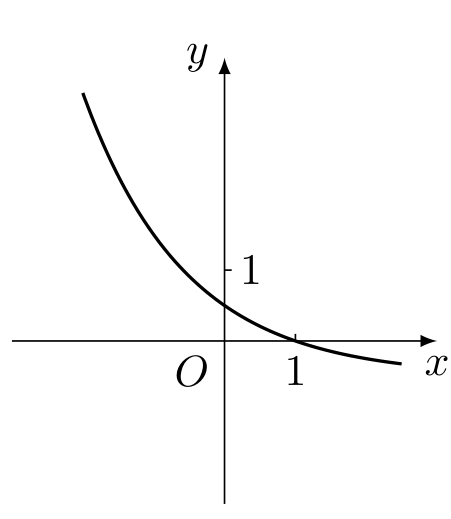
\includegraphics[width=0.15\paperwidth]{GaoKao/images/2012/sichuan_science/q5_choice_c.png}  &  \text{D. }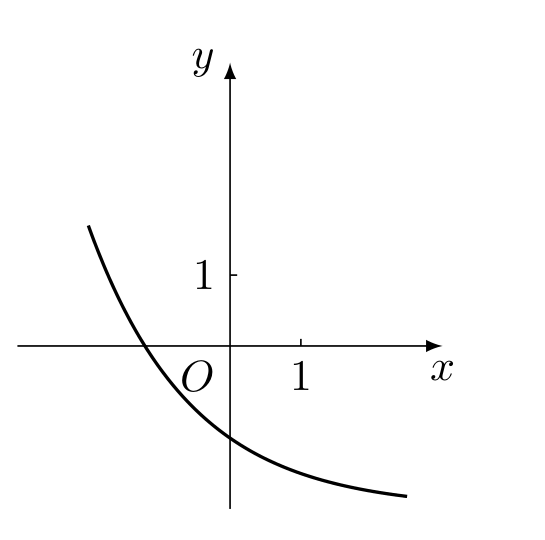
\includegraphics[width=0.15\paperwidth]{GaoKao/images/2012/sichuan_science/q5_choice_d.png}
        \end{tabular*}\par}

        \item 下列命题正确的是（\quad）

        {\centering\begin{tabular*}{\linewidth}{@{}@{\extracolsep{\fill}}llll@{}}
          \text{A. }若两条直线和同一个平面所成的角相等，则这两条直线平行  &  \text{B. }若一个平面内有三个点到另一个平面的距离相等，则这两个平面平行  &  \text{C. }若一条直线平行于两个相交平面，则这条直线与这两个平面的交线平行  &  \text{D. }若两个平面都垂直于第三个平面，则这两个平面平行
        \end{tabular*}\par}

        \item 设 \(\bm{a}\)，\(\bm{b}\) 都是非零向量. 下列四个条件中，使 \(\frac{\bm{a}}{|\bm{a}|} = \frac{\bm{b}}{|\bm{b}|}\) 成立的充分条件是（\quad）

        {\centering\begin{tabular*}{\linewidth}{@{}@{\extracolsep{\fill}}llll@{}}
          \text{A. }\(\bm{a} = -\bm{b}\)  &  \text{B. }\(\bm{a} \parallel \bm{b}\)  &  \text{C. }\(\bm{a} = 2\bm{b}\)  &  \text{D. }\(|\bm{a}| = |\bm{b}|\) 且 \(\bm{a} \parallel \bm{b}\)
        \end{tabular*}\par}

        \item 已知抛物线关于 \(x\) 轴对称，它的顶点在坐标原点 \(O\)，并且经过点 \(M(2, y_0)\). 若点 \(M\) 到该抛物线焦点的距离为 3，则 \(|OM|=\)（\quad）

        {\centering\begin{tabular*}{\linewidth}{@{}@{\extracolsep{\fill}}llll@{}}
          \text{A. }\(2\sqrt{2}\)  &  \text{B. }\(2\sqrt{3}\)  &  \text{C. }4  &  \text{D. }\(2\sqrt{5}\)
        \end{tabular*}\par}

        \item 某公司生产甲，乙两种桶装产品. 已知生产甲产品 \(1\) 桶需耗 A 原料 \(1\text{ 千克}\)，B 原料 \(2\text{ 千克}\)；生产乙产品 \(1\) 桶需耗 A 原料 \(2\text{ 千克}\)，B 原料 \(1\text{ 千克}\). 每桶甲产品的利润是 \(300\text{ 元}\). 每桶乙产品的利润是 \(400\text{ 元}\). 公司在生产这两种产品的计划中，要求每天消耗 A，B 原料都不超过 \(12\text{ 千克}\). 通过合理安排生产计划，从每天生产的甲，乙两种产品中，公司共可获得的最大利润是（\quad）

        {\centering\begin{tabular*}{\linewidth}{@{}@{\extracolsep{\fill}}llll@{}}
          \text{A. }\(1800\text{ 元}\)  &  \text{B. }\(2400\text{ 元}\)  &  \text{C. }\(2800\text{ 元}\)  &  \text{D. }\(3100\text{ 元}\)
        \end{tabular*}\par}

        \item 如图，半径为 \(R\) 的半球 \(O\) 的底面圆 \(O\) 在平面 \(\alpha\) 内，过点 \(O\) 作平面 \(\alpha\) 的垂线交半球面于点 \(A\)，过圆 \(O\) 的直径 \(CD\) 作与平面 \(\alpha\) 成 \(45^{\circ}\) 角的平面与半球面相交，所得交线上到平面 \(\alpha\) 的距离最大的点为 \(B\)，该交线上的一点 \(P\) 满足 \(\angle BOP = 60^{\circ}\)，则 \(A\)，\(P\) 两点间的球面距离为（\quad）

\begin{center}
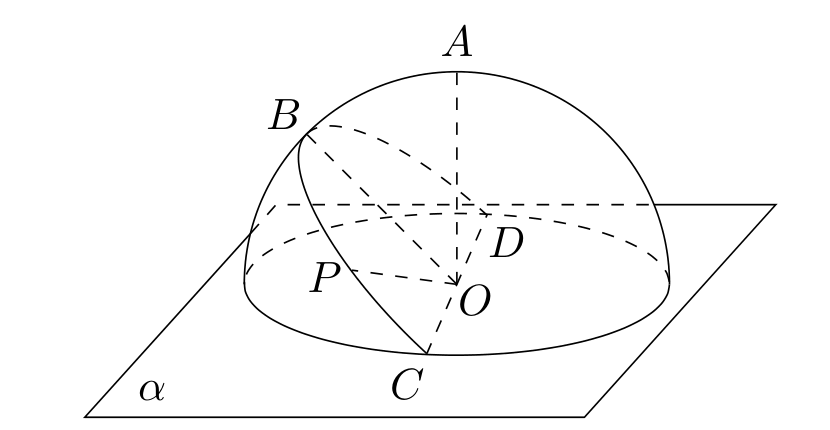
\includegraphics[width=9.0cm]{GaoKao/images/2012/sichuan_science/q10_fig1.png}
\end{center}

        {\centering\begin{tabular*}{\linewidth}{@{}@{\extracolsep{\fill}}llll@{}}
          \text{A. }\(R\arccos\frac{\sqrt{2}}{4}\)  &  \text{B. }\(\frac{\pi R}{4}\)  &  \text{C. }\(R\arccos \frac{\sqrt{3}}{3}\)  &  \text{D. }\(\frac{\pi R}{3}\)
        \end{tabular*}\par}

        \item 方程 \(ay = b^2 x^2 + c\) 中的 \(a\)，\(b\)，\(c \in \{-3, -2, 0, 1, 2, 3\}\)，且 \(a\)，\(b\)，\(c\) 互不相同，在所有这些方程所表示的曲线中，不同的抛物线共有（\quad）

        {\centering\begin{tabular*}{\linewidth}{@{}@{\extracolsep{\fill}}llll@{}}
          \text{A. }60 条  &  \text{B. }62 条  &  \text{C. }71 条  &  \text{D. }80 条
        \end{tabular*}\par}

        \item 设函数 \( f(x) = 2x - \cos x \)，\( \{a_n\} \) 是公差为 \( \frac{\pi}{8} \) 的等差数列，\( f(a_1) + f(a_2) + \cdots + f(a_5) = 5\pi \)，则 \( \left[f(a_3)\right]^2 - a_1a_5 = \)（\quad）

        {\centering\begin{tabular*}{\linewidth}{@{}@{\extracolsep{\fill}}llll@{}}
          \text{A. }0  &  \text{B. }\(\frac{1}{16}\pi^2\)  &  \text{C. }\(\frac{1}{8}\pi^2\)  &  \text{D. }\(\frac{13}{16}\pi^2\)
        \end{tabular*}\par}

    \end{enumerate}

\end{description}

\begin{description}

    \item[二、填空题]

    \begin{enumerate}[leftmargin=5pt]

      \addtocounter{enumi}{+12}

        \item 设全集 \(U = \{a, b, c, d\}\)，集合 \(A = \{a, b\}\)，\(B = \{b, c, d\}\)，则 \(\left(\complement_U A\right) \cup \left(\complement_U B\right) = \)\rule[-0.3ex]{3em}{0.4pt}.

        \item 如图，在正方体 \(ABCD - A_{1}B_{1}C_{1}D_{1}\) 中，\(M\)，\(N\) 分别是 \(CD\)，\(CC_{1}\) 的中点，则异面直线 \(A_{1}M\) 与 \(DN\) 所成角的大小是\rule[-0.3ex]{3em}{0.4pt}.

\begin{center}
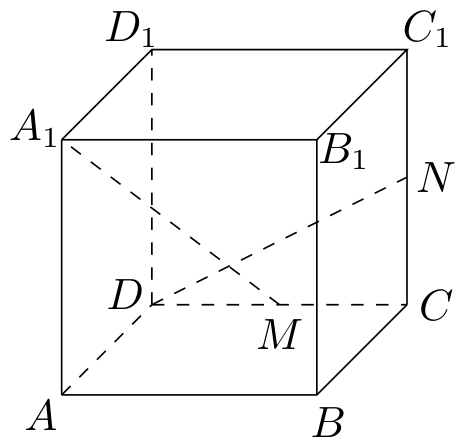
\includegraphics[width=4.9cm]{GaoKao/images/2012/sichuan_science/q14_fig1.png}
\end{center}

        \item 椭圆 \(\frac{x^2}{4} + \frac{y^2}{3} = 1\) 的左焦点为 \(F\)，直线 \(x = m\) 与椭圆相交于点 \(A\)，\(B\). 当 \(\triangle FAB\) 的周长最大时，\(\triangle FAB\) 的面积是\rule[-0.3ex]{3em}{0.4pt}.

        \item 记 \([x]\) 为不超过实数 \(x\) 的最大整数，例如，\([2]\) = \(2\)，\([1.5]\) = \(1\)，\([{-0.3}]\) = \(-1\). 设 \(a\) 为正整数，数列 \(\{x_n\}\) 满足 \(x_1 = a\)，\(x_{n+1} = \left[\dfrac{x_n + \left[\dfrac{a}{x_n}\right]}{2}\right]\)（\(n \in \mathbf{N}^*\)），现有下列命题：

\begin{enumerate}
\item 当 \(a = 5\) 时，数列 \(\{x_n\}\) 的前3项依次为 \(5\)，\(3\)，\(2\)；
\item 对数列 \(\{x_n\}\) 都存在正整数 \(k\)，当 \(n \geqslant k\) 时总有 \(x_n = x_k\)；
\item 当 \(n \geqslant 1\) 时，\(x_n > \sqrt{a} - 1\)；
\item 对某个正整数 \(k\)，若 \(x_{k + 1} \geqslant x_k\)，则 \(x_n = [\sqrt{a}]\).
\end{enumerate}

其中的真命题有\rule[-0.3ex]{3em}{0.4pt}（写出所有真命题的编号）

    \end{enumerate}

\end{description}

\begin{description}

    \item[三、解答题]

    \begin{enumerate}[leftmargin=5pt]

      \addtocounter{enumi}{+16}

        \item 某居民小区有两个相互独立的安全防范系统（简称系统） \(A\) 和 \(B\)，系统 \(A\) 和 \(B\) 在任意时刻发生故障的概率分别为 \(\frac{1}{10}\) 和 \(p\).
\begin{enumerate}
\item 若在任意时刻至少有一个系统不发生故障的概率为 \(\frac{49}{50}\)，求 \(p\) 的值；
\item 设系统 \(A\) 在 3 次相互独立的检测中不发生故障的次数为随机变量 \(\xi\)，求 \(\xi\) 的概率分布列及数学期望 \(E(\xi)\).
\end{enumerate}

        \item 函数 \(f(x)=6\cos^2\left(\frac{\omega x}{2}\right)+\sqrt{3}\sin\omega x-3\)（\(\omega>0\)）在一个周期内的图象如图所示，\(A\) 为图象的最高点，\(B\)，\(C\) 为图象与 \(x\) 轴的交点，且 \(\triangle ABC\) 为正三角形.
\begin{enumerate}
\item 求 \( \omega \) 的值及函数 \( f(x) \) 的值域；
\item 若 \( f(x_0) = \frac{8\sqrt{3}}{5} \)，且 \( x_0 \in \left(-\frac{10}{3}, \frac{2}{3}\right) \)，求 \( f(x_0 + 1) \) 的值.
\end{enumerate}

\begin{center}
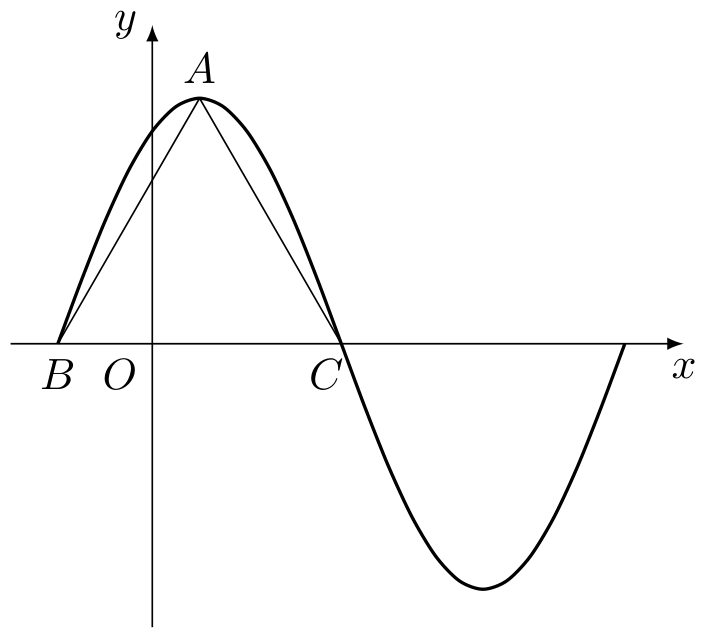
\includegraphics[width=8.5cm]{GaoKao/images/2012/sichuan_science/q18_fig1.png}
\end{center}

        \item 如图，在三棱锥 \(P - ABC\) 中，\(\angle APB = 90^{\circ}\)，\(\angle PAB = 60^{\circ}\)，\(AB = BC = CA\)，平面 \(PAB \perp\) 平面 \(ABC\).
\begin{enumerate}
\item 求直线 \(PC\) 与平面 \(ABC\) 所成角的正弦值；
\item 求二面角 \(B - AP - C\) 的余弦值.
\end{enumerate}

\begin{center}
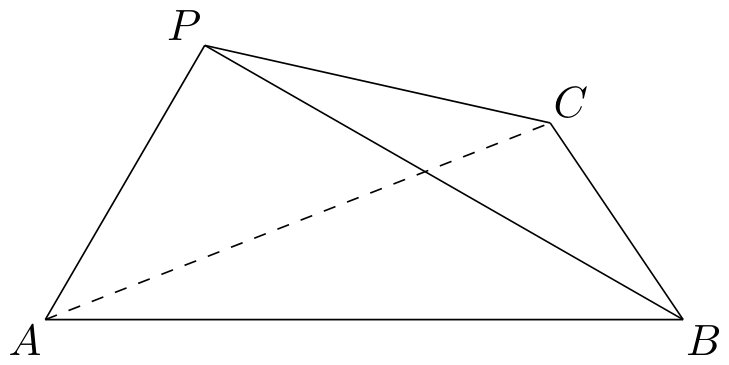
\includegraphics[width=8.8cm]{GaoKao/images/2012/sichuan_science/q19_fig1.png}
\end{center}

        \item 已知数列 \(\{a_{n}\}\) 的前 \(n\) 项和为 \(S_{n}\)，且 \(a_{2}a_{n} = S_{2} + S_{n}\) 对一切正整数 \(n\) 都成立.
\begin{enumerate}
\item 求 \(a_{1}\)，\(a_{2}\) 的值；
\item 设 \(a_{1} > 0\)，数列 \(\left\{\lg \frac{10a_{1}}{a_{n}}\right\}\) 的前 \(n\) 项和为 \(T_{n}\)，当 \(n\) 为何值时，\(T_{n}\) 最大，并求出 \(T_{n}\) 的最大值.
\end{enumerate}

        \item 如图，动点 \(M\) 与两定点 \(A(-1,0)\)，\(B(2,0)\) 构成 \(\triangle MAB\)，且 \(\angle MBA = 2\angle MAB\)，设动点 \(M\) 的轨迹为 \(C\).
\begin{enumerate}
\item 求轨迹 \(C\) 的方程；
\item 设直线 \(y = -2x + m\) 与 \(y\) 轴相交于点 \(P\)，与轨迹 \(C\) 相交于点 \(Q\)，\(R\)，且 \(|PQ| < |PR|\)，求 \(\frac{|PR|}{|PQ|}\) 的取值范围.
\end{enumerate}
\begin{center}
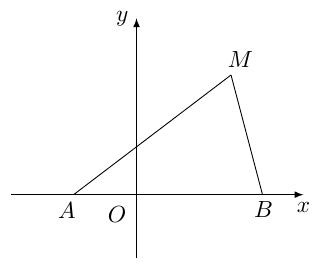
\includegraphics[width=6.8cm]{GaoKao/images/2012/sichuan_science/q21_fig1.png}
\end{center}

        \item 已知 \(a\) 为正实数，\(n\) 为自然数，抛物线 \(y = -x^{2} + \frac{a^{n}}{2}\) 与 \(x\) 轴正半轴相交于点 \(A\)，设 \(f(n)\) 为该抛物线在点 \(A\) 处切的切线在 \(y\) 轴上的截距.
\begin{enumerate}
\item 用 \(a\) 和 \(n\) 表示 \(f(n)\)；
\item 求对所有 \(n\) 都有 \(\frac{f(n) - 1}{f(n) + 1} \geqslant \frac{n^3}{n^3 + 1}\) 成立的 \(a\) 的最小值；
\item 当 \(0 < a < 1\) 时，比较 \(\sum_{k=1}^{n} \frac{f(k)}{f(k) - f(2k)}\) 与 \(\frac{27}{4} \cdot \frac{f(1) - f(n)}{f(0) - f(1)}\) 的大小，并说明理由.
\end{enumerate}

    \end{enumerate}

\end{description}


\subsection{2012年四川卷（文）}\label{gk:2012年四川卷（文）}

\begin{description}

    \item[一、选择题]

    \begin{enumerate}[leftmargin=5pt]

        \item 设集合 \(A = \{a, b\}\)，\(B = \{b, c, d\}\)，则 \(A \cup B =\)（\quad）

        {\centering\begin{tabular*}{\linewidth}{@{}@{\extracolsep{\fill}}llll@{}}
          \text{A. }\(\{b\}\)  &  \text{B. }\(\{b, c, d\}\)  &  \text{C. }\(\{a, c, d\}\)  &  \text{D. }\(\{a, b, c, d\}\)
        \end{tabular*}\par}

        \item \((1 + x)^{7}\) 的展开式中 \(x^{2}\) 的系数是（\quad）

        {\centering\begin{tabular*}{\linewidth}{@{}@{\extracolsep{\fill}}llll@{}}
          \text{A. }21  &  \text{B. }28  &  \text{C. }35  &  \text{D. }42
        \end{tabular*}\par}

        \item 交通管理部门为了解机动车驾驶员（简称驾驶员）对某新法规的知晓情况，对甲，乙，丙，丁四个社区做分层抽样调查. 假设四个社区驾驶员的总人数为 \(N\)，其中甲社区有驾驶员 \(96\) 人. 若在甲，乙，丙，丁四个社区抽取驾驶员的人数分别为 \(12\)、\(21\)、\(25\)、\(43\)，则这四个社区驾驶员的总人数 \(N\) 为（\quad）

        {\centering\begin{tabular*}{\linewidth}{@{}@{\extracolsep{\fill}}llll@{}}
          \text{A. }101  &  \text{B. }808  &  \text{C. }1212  &  \text{D. }2012
        \end{tabular*}\par}

        \item 函数 \( y = a^x - a \) （\( a > 0 \)，且 \( a \neq 1 \)） 的图象可能是（\quad）

        {\centering\begin{tabular*}{\linewidth}{@{}@{\extracolsep{\fill}}cccc@{}}
          \text{A. }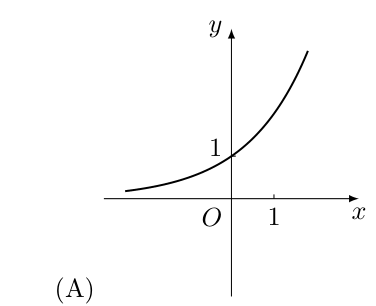
\includegraphics[width=0.15\paperwidth]{GaoKao/images/2012/sichuan_liberal/q4_A.png}  &  \text{B. }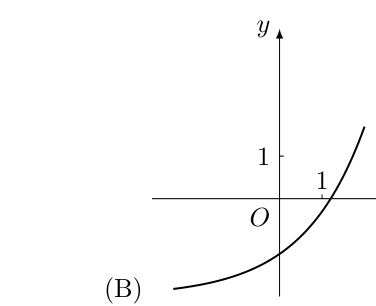
\includegraphics[width=0.15\paperwidth]{GaoKao/images/2012/sichuan_liberal/q4_B.png}  &  \text{C. }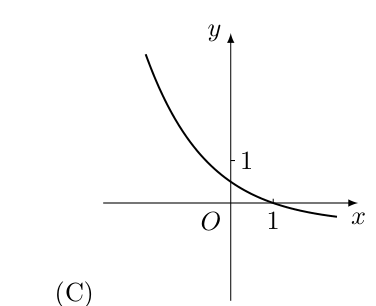
\includegraphics[width=0.15\paperwidth]{GaoKao/images/2012/sichuan_liberal/q4_C.png}  &  \text{D. }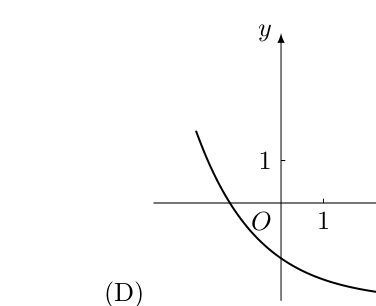
\includegraphics[width=0.15\paperwidth]{GaoKao/images/2012/sichuan_liberal/q4_D.png}
        \end{tabular*}\par}

        \item 如图，正方形 \(ABCD\) 的边长为 \(1\)，延长 \(BA\) 至 \(E\)，使 \(AE = 1\)，连接 \(EC\)，\(ED\)，则 \(\sin \angle CED =\)（\quad）

\begin{center}
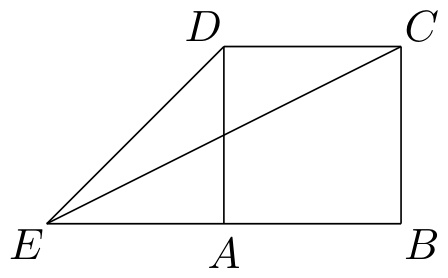
\includegraphics[width=5.6cm]{GaoKao/images/2012/sichuan_liberal/q5_fig1.png}
\end{center}

        {\centering\begin{tabular*}{\linewidth}{@{}@{\extracolsep{\fill}}llll@{}}
          \text{A. }\(\frac{3\sqrt{10}}{10}\)  &  \text{B. }\(\frac{\sqrt{10}}{10}\)  &  \text{C. }\(\frac{\sqrt{5}}{10}\)  &  \text{D. }\(\frac{\sqrt{5}}{15}\)
        \end{tabular*}\par}

        \item 下列命题正确的是（\quad）

        {\centering\begin{tabular*}{\linewidth}{@{}@{\extracolsep{\fill}}llll@{}}
          \text{A. }若两条直线和同一个平面所成的角相等，则这两条直线平行  &  \text{B. }若一个平面内有三个点到另一个平面的距离相等，则这两个平面平行  &  \text{C. }若一条直线平行于两个相交平面，则这条直线与这两个平面的交线平行  &  \text{D. }若两个平面都垂直于第三个平面，则这两个平面平行
        \end{tabular*}\par}

        \item 设 \(\bm{a}\)，\(\bm{b}\) 都是非零向量. 下列四个条件中，使 \( \frac{\bm{a}}{|\bm{a}|} = \frac{\bm{b}}{|\bm{b}|} \) 成立的充分条件是（\quad）

        {\centering\begin{tabular*}{\linewidth}{@{}@{\extracolsep{\fill}}llll@{}}
          \text{A. }\(|\bm{a}| = |\bm{b}|\) 且 \(\bm{a}\parallel\bm{b}\)  &  \text{B. }\(\bm{a} = -\bm{b}\)  &  \text{C. }\(\bm{a}\parallel\bm{b}\)  &  \text{D. }\(\bm{a} = 2\bm{b}\)
        \end{tabular*}\par}

        \item 若变量 \(x\)，\(y\) 满足约束条件 \(\begin{cases}
x - y \geqslant -3,\\
x + 2y \leqslant 12,\\
2x + y \leqslant 12,\\
x \geqslant 0,\\
y \geqslant 0,
\end{cases}\) 则 \(z = 3x + 4y\) 的最大值是（\quad）

        {\centering\begin{tabular*}{\linewidth}{@{}@{\extracolsep{\fill}}llll@{}}
          \text{A. }12  &  \text{B. }26  &  \text{C. }28  &  \text{D. }33
        \end{tabular*}\par}

        \item 已知抛物线关于 \(x\) 轴对称，它的顶点在坐标原点 \(O\)，并且经过点 \(M(2, y_0)\). 若点 \(M\) 到该抛物线焦点的距离为 3，则 \(|OM| =\)（\quad）

        {\centering\begin{tabular*}{\linewidth}{@{}@{\extracolsep{\fill}}llll@{}}
          \text{A. }\(2\sqrt{2}\)  &  \text{B. }\(2\sqrt{3}\)  &  \text{C. }4  &  \text{D. }\(2\sqrt{5}\)
        \end{tabular*}\par}

        \item 如图，半径为 \(R\) 的球 \(O\) 的底面圆 \(O\) 在平面 \(\alpha\) 内，过点 \(O\) 作平面 \(\alpha\) 的垂线交球面于点 \(A\)，过点 \(O\) 的直径 \(CD\) 与平面 \(\alpha\) 成 \(45^{\circ}\) 的平面与球面相交，所得交线上到平面 \(\alpha\) 的距离最大的点为 \(B\)，该交线上的一点 \(P\) 满足 \(\angle BOP=60^{\circ}\)，则 \(A\)，\(P\) 两点间的球面距离为（\quad）

\begin{center}
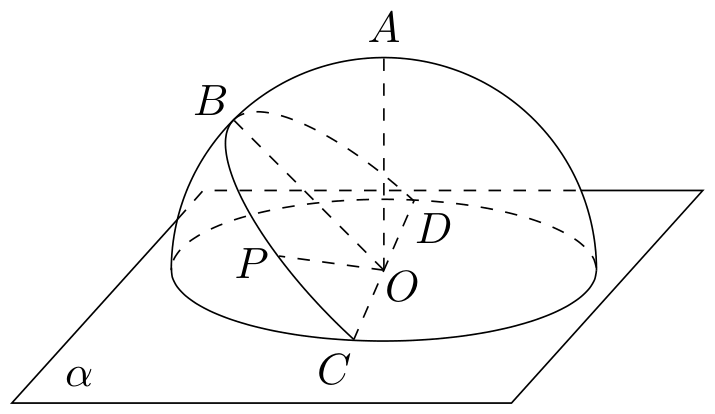
\includegraphics[width=12.3cm]{GaoKao/images/2012/sichuan_liberal/q10_fig1.png}
\end{center}

        {\centering\begin{tabular*}{\linewidth}{@{}@{\extracolsep{\fill}}llll@{}}
          \text{A. }\(R\arccos\frac{\sqrt{2}}{4}\)  &  \text{B. }\(\frac{\pi R}{4}\)  &  \text{C. }\(R\arccos\frac{\sqrt{3}}{3}\)  &  \text{D. }\(\frac{\pi R}{3}\)
        \end{tabular*}\par}

        \item 方程 \(ay = b^2 x^2 + c\) 中的 \(a\)，\(b\)，\(c \in \{-2, 0, 1, 2, 3\}\)，且 \(a\)，\(b\)，\(c\) 互不相同. 在所有这些方程所表示的曲线中，不同的抛物线共有（\quad）

        {\centering\begin{tabular*}{\linewidth}{@{}@{\extracolsep{\fill}}llll@{}}
          \text{A. }28 条  &  \text{B. }32 条  &  \text{C. }36 条  &  \text{D. }48 条
        \end{tabular*}\par}

        \item 设函数 \( f(x) = (x - 3)^3 + x - 1 \)，\( \{a_n\} \) 是公差不为 0 的等差数列，\( f(a_1) + f(a_2) + \dots + f(a_7) = 14 \)，则 \( a_1 + a_2 + \dots + a_7 = \)（\quad）

        {\centering\begin{tabular*}{\linewidth}{@{}@{\extracolsep{\fill}}llll@{}}
          \text{A. }0  &  \text{B. }7  &  \text{C. }14  &  \text{D. }21
        \end{tabular*}\par}

    \end{enumerate}

\end{description}

\begin{description}

    \item[二、填空题]

    \begin{enumerate}[leftmargin=5pt]

      \addtocounter{enumi}{+12}

        \item 函数 \( f(x) = \frac{1}{\sqrt{1 - 2x}} \) 的定义域是\rule[-0.3ex]{3em}{0.4pt}（用区间表示）.

        \item 如图，在正方体 \(ABCD - A_{1}B_{1}C_{1}D_{1}\) 中，\(M\)，\(N\) 分别是 \(CD\)，\(CC_{1}\) 的中点，则异面直线 \(A_{1}M\) 与 \(DN\) 所成角的大小是\rule[-0.3ex]{3em}{0.4pt}.
\begin{center}
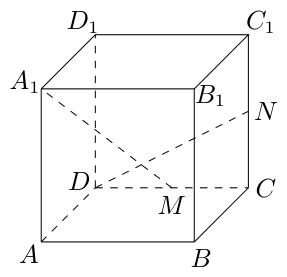
\includegraphics[width=4.8cm]{GaoKao/images/2012/sichuan_liberal/q14_fig1.png}
\end{center}

        \item 椭圆 \(\frac{x^2}{a^2} + \frac{y^2}{5} = 1\)（\(a\) 为定值，且 \(a > \sqrt{5}\)）的左焦点为 \(F\)，直线 \(x = m\) 与椭圆相交于点 \(A\)，\(B\)，\(\triangle FAB\) 的周长的最大值是 12，则该椭圆的离心率是\rule[-0.3ex]{3em}{0.4pt}.

        \item 设 \(a\)，\(b\) 为正实数. 现有下列命题：
\begin{enumerate}
\item 若 \(a^2 - b^2 = 1\)，则 \(a - b < 1\)；
\item 若 \(\frac{1}{b} -\frac{1}{a} = 1\)，则 \(a - b < 1\)；
\item 若 \(|\sqrt{a} - \sqrt{b}| = 1\)，则 \(|a - b| < 1\)；
\item 若 \( |a^3 - b^3| = 1 \)，
\end{enumerate}
则 \( |a - b| < 1 \). 其中的真命题有\rule[-0.3ex]{3em}{0.4pt}（写出所有真命题的编号）.

    \end{enumerate}

\end{description}

\begin{description}

    \item[三、解答题]

    \begin{enumerate}[leftmargin=5pt]

      \addtocounter{enumi}{+16}

        \item 某居民小区有两个相互独立的安全防范系统（简称系统）\(A\) 和 \(B\)，系统 \(A\) 和 \(B\) 在任意时刻发生故障的概率分别为 \( \frac{1}{10} \) 和 \(p\).
\begin{enumerate}
\item 若在任意时刻至少有一个系统不发生故障的概率为 \(\frac{49}{50}\)，求 \(p\) 的值；
\item 求系统 \(A\) 在 3 次相互独立的检测中不发生故障的次数大于发生故障的次数的概率.
\end{enumerate}

        \item 已知函数 \( f(x) = \cos^2\frac{x}{2} - \sin \frac{x}{2}\cos \frac{x}{2} - \frac{1}{2} \).
\begin{enumerate}
\item 求函数 \( f(x) \) 的最小正周期和值域.
\item 若 \( f(\alpha)=\frac{3\sqrt{2}}{10} \)，求 \( \sin 2\alpha \) 的值.
\end{enumerate}

        \item 如图，在三棱锥 \(P - ABC\) 中，\(\angle APB = 90^{\circ}\)，\(\angle PAB = 60^{\circ}\)，\(AB = BC = CA\)，点 \(P\) 在平面 \(ABC\) 内的射影 \(O\) 在 \(AB\) 上.
\begin{enumerate}
\item 求直线 \(PC\) 与平面 \(ABC\) 所成角的正弦值；
\item 求二面角 \(B - AP - C\) 的余弦值.
\end{enumerate}
\begin{center}
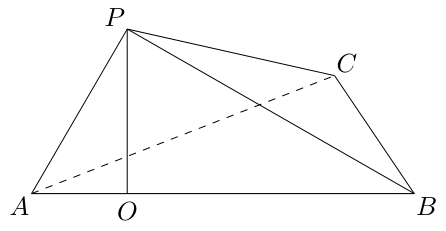
\includegraphics[width=8.7cm]{GaoKao/images/2012/sichuan_liberal/q19_fig1.png}
\end{center}

        \item 已知数列 \(\{a_{n}\}\) 的前 \(n\) 项和为 \(S_{n}\)，常数 \(\lambda > 0\)，且 \(\lambda a_{1}a_{n} = S_{1} + S_{n}\). 对一切正整数 \(n\) 都成立.
\begin{enumerate}
\item 求数列 \( \{a_{n}\} \) 的通项公式；
\item 设 \(a_{1} > 0\)，\(\lambda = 100\). 当 \(n\) 为何值时，数列 \(\left\{\lg \frac{1}{a_n}\right\}\) 的前 \(n\) 项和最大.
\end{enumerate}

        \item 如图，动点 \(M\) 与两定点 \(A(-1,0)\)，\(B(1,0)\) 构成 \(\triangle MAB\)，且直线 \(MA\)，\(MB\) 的斜率之积为 \(4\). 设动点 \(M\) 的轨迹为 \(C\).
\begin{enumerate}
\item 求轨迹 \(C\) 的方程；
\item 设直线 \( y = x + m \) （\( m > 0 \)） 与 \( y \) 轴相交于点 \(P\). 与轨迹 \(C\) 相交于点 \(Q\)，\(R\)，且 \( |PQ| < |PR| \)，求 \( \frac{|PR|}{|PQ|} \) 的取值范围.
\end{enumerate}
\begin{center}
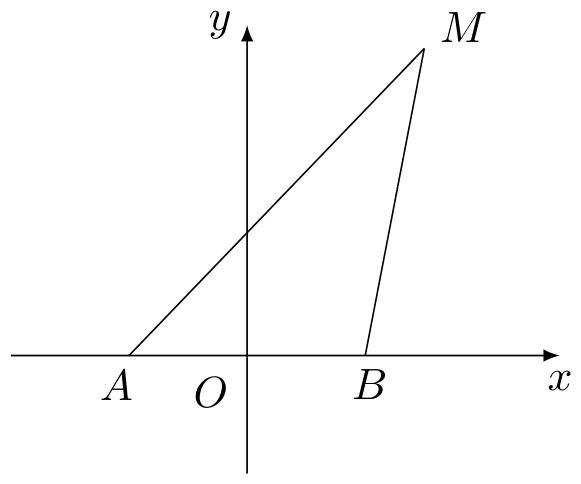
\includegraphics[width=6.8cm]{GaoKao/images/2012/sichuan_liberal/q21_fig1.png}
\end{center}

        \item 已知 \(a\) 为正实数，\(n\) 为自然数，抛物线 \(y = -x^{2} + \frac{a^{n}}{2}\) 与 \(x\) 轴正半轴相交于点 \(A\). 设 \(f(n)\) 为该抛物线在点 \(A\) 处的切线在 \(y\) 轴上的截距.
\begin{enumerate}
\item 用 \(a\) 和 \(n\) 表示 \( f(n) \)；
\item 求对所有 \(n\) 都有 \(\frac{f(n) - 1}{f(n) + 1} \geqslant \frac{n}{n + 1}\) 成立的 \(a\) 的最小值；
\item 当 \(0 < a < 1\) 时，比较 \(\frac{1}{f(1) - f(2)} + \frac{1}{f(2) - f(4)} + \cdots + \frac{1}{f(n) - f(2n)}\) 与 \(6 \cdot \frac{f(1) - f(n + 1)}{f(0) - f(1)}\) 的大小，并说明理由.
\end{enumerate}

    \end{enumerate}

\end{description}


\subsection{2012年山东卷（理）}\label{gk:2012年山东卷（理）}

\begin{description}

    \item[一、选择题]

    \begin{enumerate}[leftmargin=5pt]

        \item 若复数 \(z\) 满足 \(z(2 - \i) = 11 + 7\i\) （\(\i\) 为虚数单位），则 \(z\) 为（\quad）

        {\centering\begin{tabular*}{\linewidth}{@{}@{\extracolsep{\fill}}llll@{}}
          \text{A. }\(3 + 5\i\)  &  \text{B. }\(3 - 5\i\)  &  \text{C. }\(-3 + 5\i\)  &  \text{D. }\(-3 - 5\i\)
        \end{tabular*}\par}

        \item 已知全集 \(U = \{0, 1, 2, 3, 4\}\)，集合 \(A = \{1, 2, 3\}\)，\(B = \{2, 4\}\)，则 \(\complement_U A \cup B =\)（\quad）

        {\centering\begin{tabular*}{\linewidth}{@{}@{\extracolsep{\fill}}llll@{}}
          \text{A. }\(\{1, 2, 4\}\)  &  \text{B. }\(\{2, 3, 4\}\)  &  \text{C. }\(\{0, 2, 4\}\)  &  \text{D. }\(\{0, 2, 3, 4\}\)
        \end{tabular*}\par}

        \item 设 \(a > 0\) 且 \(a \neq 1\)，则“函数 \(f(x) = a^x\) 在 \(\mathbb{R}\) 上是减函数”是“函数 \(g(x) = (2 - a)x^3\) 在 \(\mathbb{R}\) 上是增函数”的（\quad）

        {\centering\begin{tabular*}{\linewidth}{@{}@{\extracolsep{\fill}}llll@{}}
          \text{A. }充分不必要条件  &  \text{B. }必要不充分条件  &  \text{C. }充分必要条件  &  \text{D. }既不充分也不必要条件
        \end{tabular*}\par}

        \item 采用系统抽样方法从 960 人中抽取 32 人做问卷调查. 为此将他们随机编号为 1, 2, \ldots, 960，分组后在第一组采用简单随机抽样的方法抽到的号码为 9. 抽到的 32 人中，编号落入区间 \([1, 450]\) 的人做问卷 A，编号落入区间 \([451, 750]\) 的人做问卷 B，其余的人做问卷 C. 则抽到的人中，做问卷 B 的人数为（\quad）

        {\centering\begin{tabular*}{\linewidth}{@{}@{\extracolsep{\fill}}llll@{}}
          \text{A. }7  &  \text{B. }9  &  \text{C. }10  &  \text{D. }15
        \end{tabular*}\par}

        \item 设变量 \(x\)，\(y\) 满足约束条件 \(\begin{cases}
x + 2y \geqslant 2,\\
2x + y \leqslant 4,\\
4x - y \geqslant -1,
\end{cases}\) 则目标函数 \(z = 3x - y\) 的取值范围是（\quad）

        {\centering\begin{tabular*}{\linewidth}{@{}@{\extracolsep{\fill}}llll@{}}
          \text{A. }\(\left[\frac{3}{2}, 6\right]\)  &  \text{B. }\(\left[-\frac{3}{2}, -1\right]\)  &  \text{C. }\([-1,6]\)  &  \text{D. }\(\left[-6, \frac{3}{2}\right]\)
        \end{tabular*}\par}

        \item 执行如图所示的程序框图，如果输入 \(a = 4\)，那么输出的 \(n\) 的值为（\quad）

\begin{center}
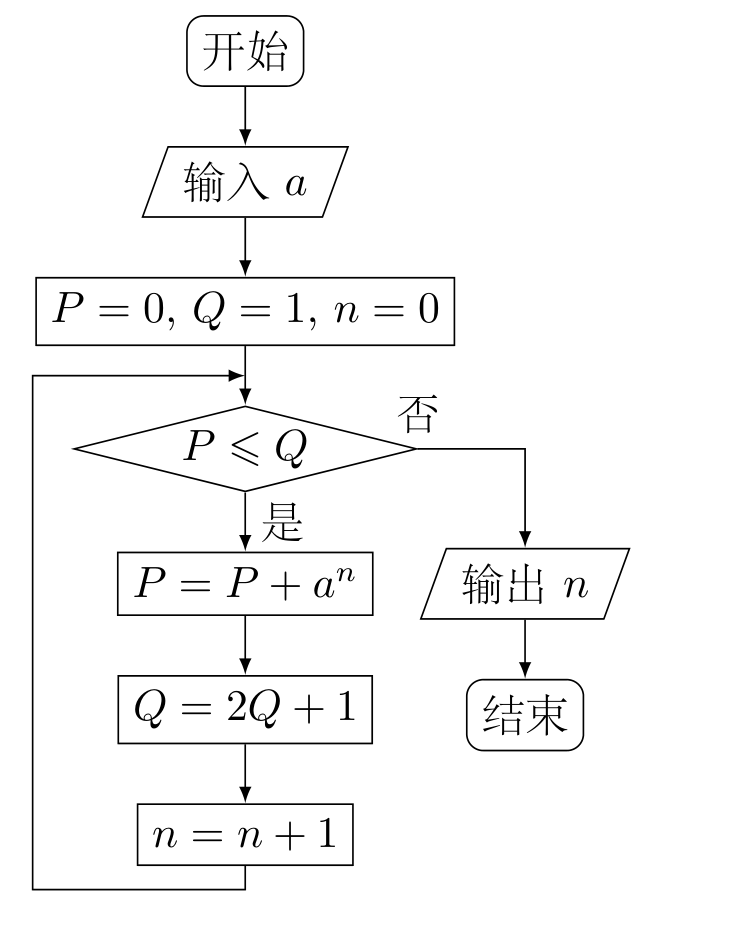
\includegraphics[width=0.60\linewidth]{GaoKao/images/2012/shandong_science/q6_fig1.png}
\end{center}

        {\centering\begin{tabular*}{\linewidth}{@{}@{\extracolsep{\fill}}llll@{}}
          \text{A. }2  &  \text{B. }3  &  \text{C. }4  &  \text{D. }5
        \end{tabular*}\par}

        \item 若 \(\theta \in \left[\frac{\pi}{4}, \frac{\pi}{2}\right]\)，\(\sin 2\theta = \frac{3\sqrt{7}}{8}\)，则 \(\sin \theta =\)（\quad）

        {\centering\begin{tabular*}{\linewidth}{@{}@{\extracolsep{\fill}}llll@{}}
          \text{A. }\(\frac{3}{5}\)  &  \text{B. }\(\frac{4}{5}\)  &  \text{C. }\(\frac{\sqrt{7}}{4}\)  &  \text{D. }\(\frac{3}{4}\)
        \end{tabular*}\par}

        \item 定义在 \(\mathbb{R}\) 的函数 \(f(x)\) 满足 \(f(x + 6) = f(x)\). 当 \(-3 \leqslant x < -1\) 时，\(f(x) = -(x + 2)^2\)；当 \(-1 \leqslant x < 3\) 时，\(f(x) = x\). 则 \(f(1) + f(2) + \cdots + f(2012) =\)（\quad）

        {\centering\begin{tabular*}{\linewidth}{@{}@{\extracolsep{\fill}}llll@{}}
          \text{A. }335  &  \text{B. }338  &  \text{C. }1678  &  \text{D. }2012
        \end{tabular*}\par}

        \item 函数 \( f(x) = \frac{\cos 6x}{2^x - 2^{-x}} \) 的图象大致为（\quad）

        {\centering\begin{tabular*}{\linewidth}{@{}@{\extracolsep{\fill}}cccc@{}}
          \text{A. }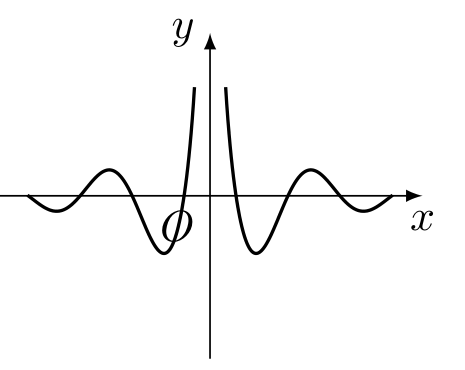
\includegraphics[width=0.15\paperwidth]{GaoKao/images/2012/shandong_science/q9_choice_a.png}  &  \text{B. }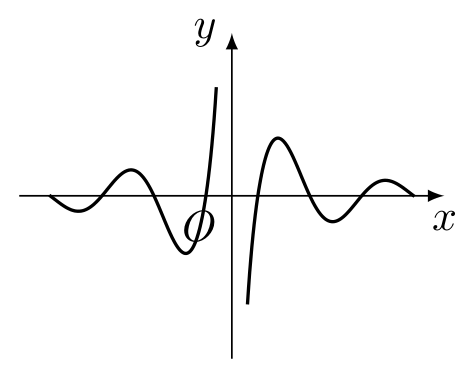
\includegraphics[width=0.15\paperwidth]{GaoKao/images/2012/shandong_science/q9_choice_b.png}  &  \text{C. }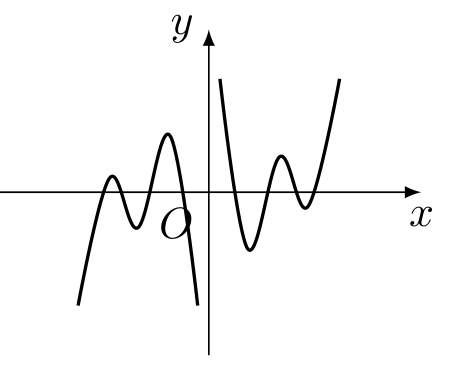
\includegraphics[width=0.15\paperwidth]{GaoKao/images/2012/shandong_science/q9_choice_c.png}  &  \text{D. }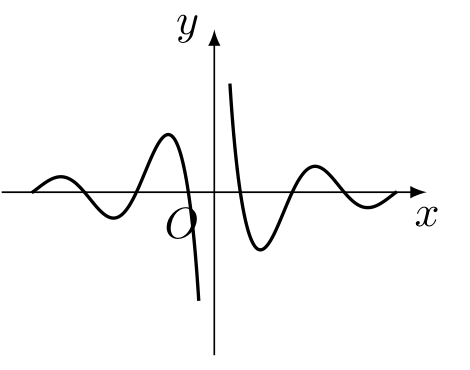
\includegraphics[width=0.15\paperwidth]{GaoKao/images/2012/shandong_science/q9_choice_d.png}
        \end{tabular*}\par}

        \item 已知椭圆 \(C: \frac{x^2}{a^2} + \frac{y^2}{b^2} = 1\) （\(a > b > 0\)） 的离心率为 \(\frac{\sqrt{3}}{2}\). 双曲线 \(x^2 - y^2 = 1\) 的渐近线与椭圆 \(C\) 有四个交点，以这四个交点为顶点的四边形的面积为 16，则椭圆 \(C\) 的方程为（\quad）

        {\centering\begin{tabular*}{\linewidth}{@{}@{\extracolsep{\fill}}llll@{}}
          \text{A. }\(\frac{x^2}{8} + \frac{y^2}{2} = 1\)  &  \text{B. }\(\frac{x^2}{12} + \frac{y^2}{6} = 1\)  &  \text{C. }\(\frac{x^2}{16} + \frac{y^2}{4} = 1\)  &  \text{D. }\(\frac{x^2}{20} + \frac{y^2}{5} = 1\)
        \end{tabular*}\par}

        \item 现有 16 张不同的卡片，其中红色、黄色、蓝色、绿色卡片各 4 张，从中任取 3 张. 要求这 3 张卡片不能是同一种颜色，且红色卡片至多 1 张. 不同的取法种数为（\quad）

        {\centering\begin{tabular*}{\linewidth}{@{}@{\extracolsep{\fill}}llll@{}}
          \text{A. }232  &  \text{B. }252  &  \text{C. }472  &  \text{D. }484
        \end{tabular*}\par}

        \item 设函数 \( f(x) = \frac{1}{x} \)，\( g(x) = ax^2 + bx\) （\(a, b \in \mathbb{R}, a \neq 0\)）. 若 \( y = f(x) \) 的图象与 \( y = g(x) \) 图象有且仅有两个不同的公共点 \(A(x_1, y_1)\)，\(B(x_2, y_2)\)，则下列判断正确的是（\quad）

        {\centering\begin{tabular*}{\linewidth}{@{}@{\extracolsep{\fill}}llll@{}}
          \text{A. }当 \(a < 0\) 时，\(x_{1} + x_{2} < 0\)，\(y_{1} + y_{2} > 0\)  &  \text{B. }当 \(a < 0\) 时，\(x_{1} + x_{2} > 0\)，\(y_{1} + y_{2} < 0\)  &  \text{C. }当 \(a > 0\) 时，\(x_{1} + x_{2} < 0\)，\(y_{1} + y_{2} < 0\)  &  \text{D. }当 \(a > 0\) 时，\(x_{1} + x_{2} > 0\)，\(y_{1} + y_{2} > 0\)
        \end{tabular*}\par}

    \end{enumerate}

\end{description}

\begin{description}

    \item[二、填空题]

    \begin{enumerate}[leftmargin=5pt]

      \addtocounter{enumi}{+12}

        \item 若不等式 \(|kx - 4| \leqslant 2\) 的解集为 \(\{x \mid 1 \leqslant x \leqslant 3\}\)，则实数 \(k = \)\rule[-0.3ex]{3em}{0.4pt}.

        \item 如图，正方体 \(ABCD - A_{1}B_{1}C_{1}D_{1}\) 的棱长为 1，\(E\)，\(F\) 分别为线段 \(AA_{1}\)，\(B_{1}C\) 上的点，则三棱锥 \(D_{1} - EDF\) 的体积为\rule[-0.3ex]{3em}{0.4pt}.

\begin{center}
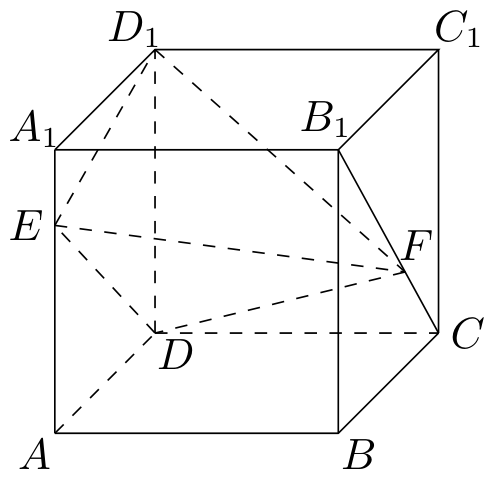
\includegraphics[width=5.3cm]{GaoKao/images/2012/shandong_science/q14_fig1.png}
\end{center}

        \item 设 \(a > 0\)，若曲线 \(y = \sqrt{x}\) 与直线 \(x = a\)，\(y = 0\) 所围成封闭图形的面积为 \(a^2\)，则 \(a = \)\rule[-0.3ex]{3em}{0.4pt}.

        \item 如图，在平面直角坐标系 \(xOy\) 中，一单位圆的圆心的初始位置在 \((0, 1)\)，此时圆上一点 \(P\) 的位置在 \((0, 0)\). 圆在 \(x\) 轴上沿正向滚动. 当圆滚动到圆心位于 \((2, 1)\) 时，\(\overrightarrow{OP}\) 的坐标为\rule[-0.3ex]{3em}{0.4pt}.

\begin{center}
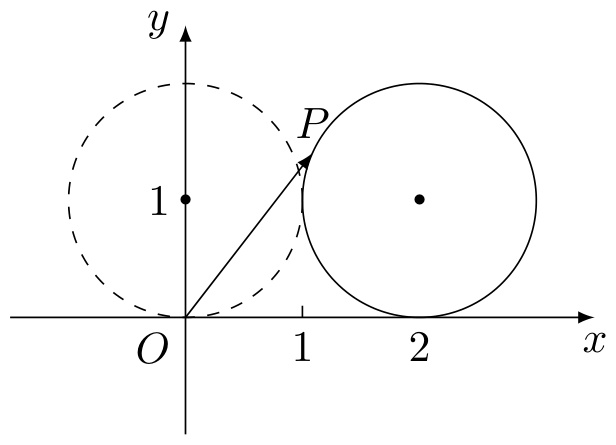
\includegraphics[width=6.0cm]{GaoKao/images/2012/shandong_science/q16_fig1.png}
\end{center}

    \end{enumerate}

\end{description}

\begin{description}

    \item[三、解答题]

    \begin{enumerate}[leftmargin=5pt]

      \addtocounter{enumi}{+16}

        \item 已知向量 \(\bm{m} = (\sin x, 1)\)，\(\bm{n} = (\sqrt{3}A \cos x, \frac{A}{2} \cos 2x)\)（\(A > 0\)），函数 \(f(x) = \bm{m} \cdot \bm{n}\) 的最大值为 6.
\begin{enumerate}
\item 求 \(A\)；
\item 将函数 \(y = f(x)\) 的图象向左平移 \(\frac{\pi}{12}\) 个单位，再将所得图象上各点的横坐标缩短为原来的 \(\frac{1}{2}\) 倍，纵坐标不变，得到函数 \(y = g(x)\) 的图象，求 \(g(x)\) 在 \(\left[0, \frac{5\pi}{24}\right]\) 上的值域.
\end{enumerate}

        \item 在如图所示的几何体中，四边形 \(ABCD\) 是等腰梯形，\(AB \parallel CD\)，\(\angle DAB = 60^{\circ}\)，\(FC \perp\) 平面 \(ABCD\)，\(AE \perp BD\)，\(CB = CD = CF\).
\begin{enumerate}
\item 求证： \(BD \perp\) 平面 \(AED\)；
\item 求二面角 \(F - BD - C\) 的余弦值.
\end{enumerate}

\begin{center}
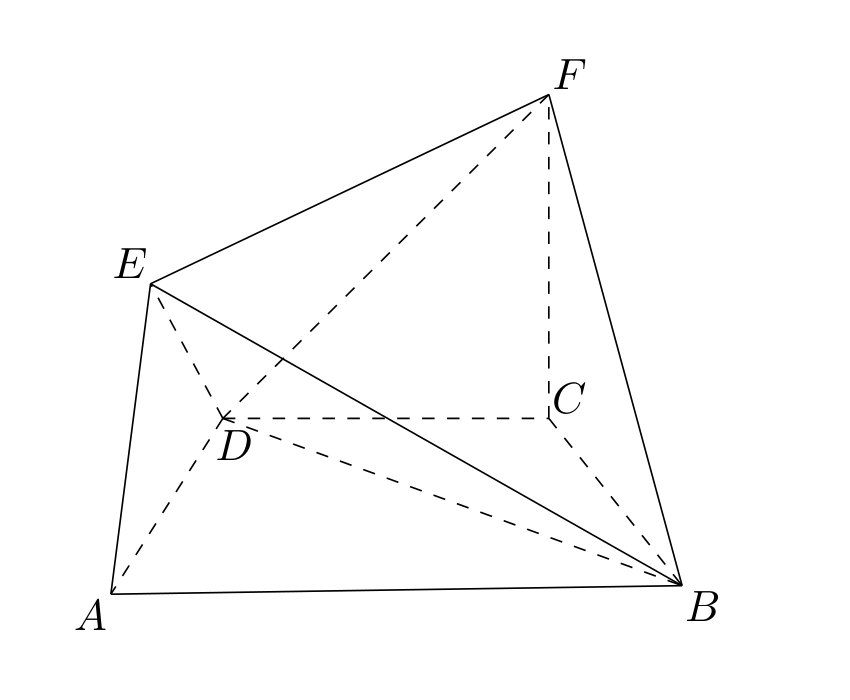
\includegraphics[width=8.0cm]{GaoKao/images/2012/shandong_science/q18_fig1.png}
\end{center}

        \item 在等差数列 \(\{a_{n}\}\) 中，\(a_{3} + a_{4} + a_{5} = 84\)，\(a_{9} = 73\).
\begin{enumerate}
\item 求数列 \(\{a_{n}\}\) 的通项公式；
\item 对任意 \(m \in \mathbf{N}^*\)，将数列 \(\{a_n\}\) 中落入区间 \((9^m, 9^{2m})\) 内的项的个数记为 \(b_m\)，求数列 \(\{b_m\}\) 的前 \(m\) 项和 \(S_m\).
\end{enumerate}

        \item 已知函数 \( f(x) = \frac{\ln x + k}{x} \)（\(k\) 为常数，\({\mathrm{e}} = 2.71828 \cdots\) 是自然对数的底数），曲线 \( y = f(x) \) 在点 \( (1, f(1)) \) 处的切线与 \( x \) 轴平行.
\begin{enumerate}
\item 求 \(k\) 的值；
\item 求 \( f(x) \) 的单调区间；
\item 设 \( g(x) = (x^2 + x)f'(x) \)，其中 \( f'(x) \) 为 \( f(x) \) 的导函数. 证明：对任意 \(x > 0\)，\(g(x) < 1 + {\mathrm{e}}^{-2}\).
\end{enumerate}

        \item 现有甲乙两个靶，某射手向甲靶射击一次命中的概率为 \(\frac{3}{4}\)，命中得 1 分，没有命中得 0 分；向乙靶射击两次，每次命中的概率为 \(\frac{2}{3}\)，每命中一次得 2 分，没有命中得 0 分. 该射手每次射击的结果相互独立，假设该射手完成以上三次射击.
\begin{enumerate}
\item 求该射手恰好命中一次的概率；
\item 求该射手的总得分 \(X\) 的分布列及数学期望 \(E(X)\).
\end{enumerate}

        \item 在平面直角坐标系 \(xOy\) 中，\(F\) 是抛物线 \(C: x^2 = 2py\) （\(p > 0\)） 的焦点，\(M\) 是抛物线 \(C\) 上位于第一象限内的任意一点，过 \(M\)，\(F\)，\(O\) 三点的圆的圆心为 \(Q\)，点 \(Q\) 到抛物线 \(C\) 的准线的距离为 \(\frac{3}{4}\).
\begin{enumerate}
\item 求抛物线 \(C\) 的方程；
\item 是否存在点 \(M\)，使得直线 \(MQ\) 与抛物线 \(C\) 相切于点 \(M\)？ 若存在，求出点 \(M\) 的坐标；若不存在，说明理由；
\item 若点 \(M\) 的横坐标为 \(\sqrt{2}\)，直线 \(l: y = kx + \frac{1}{4}\) 与抛物线 \(C\) 有两个不同的交点 \(A\)，\(B\)，\(l\) 与圆 \(Q\) 有两个不同的交点 \(D\)，\(E\)，求当 \(\frac{1}{2} \leqslant k \leqslant 2\) 时，\(|AB|^2 + |DE|^2\) 的最小值.
\end{enumerate}

    \end{enumerate}

\end{description}


\subsection{2012年山东卷（文）}\label{gk:2012年山东卷（文）}

\begin{description}

    \item[一、选择题]

    \begin{enumerate}[leftmargin=5pt]

        \item 若复数 \(z\) 满足 \(z(2 - \i) = 11 + 7\i\) （\(\i\) 为虚数单位），则 \(z\) 为（\quad）

        {\centering\begin{tabular*}{\linewidth}{@{}@{\extracolsep{\fill}}llll@{}}
          \text{A. }\(3 + 5\i\)  &  \text{B. }\(3 - 5\i\)  &  \text{C. }\(-3 + 5\i\)  &  \text{D. }\(-3 - 5\i\)
        \end{tabular*}\par}

        \item 已知全集 \(U = \{0, 1, 2, 3, 4\}\)，集合 \(A = \{1, 2, 3\}\)，\(B = \{2, 4\}\). 则 \(\left(\complement_U A\right) \cup B =\)（\quad）

        {\centering\begin{tabular*}{\linewidth}{@{}@{\extracolsep{\fill}}llll@{}}
          \text{A. }\(\{1, 2, 4\}\)  &  \text{B. }\(\{2,3,4\}\)  &  \text{C. }\(\{0,2,4\}\)  &  \text{D. }\(\{0,2,3,4\}\)
        \end{tabular*}\par}

        \item 函数 \( f(x) = \frac{1}{\ln (x + 1)} + \sqrt{4 - x^2} \) 的定义域为（\quad）

        {\centering\begin{tabular*}{\linewidth}{@{}@{\extracolsep{\fill}}llll@{}}
          \text{A. }\([-2,0)\cup (0,2]\)  &  \text{B. }\((-1,0)\cup (0,2]\)  &  \text{C. }\([-2, 2]\)  &  \text{D. }\((-1, 2]\)
        \end{tabular*}\par}

        \item 在某次测量中得到的 \(A\) 样本数据如下：82， 84， 84， 86， 86， 86， 88， 88， 88， 88. 若 \(B\) 样本数据恰好是 \(A\) 样本数据每个都加 2 后所得数据，则 \(A\)，\(B\) 两样本的下列数字特征对应相同的是（\quad）

        {\centering\begin{tabular*}{\linewidth}{@{}@{\extracolsep{\fill}}llll@{}}
          \text{A. }众数  &  \text{B. }平均数  &  \text{C. }中位数  &  \text{D. }标准差
        \end{tabular*}\par}

        \item 设命题 \(p\)：函数 \(y = \sin 2x\) 的最小正周期为 \(\frac{\pi}{2}\)；命题 \(q\)：函数 \(y = \cos x\) 的图象关于直线 \(x = \frac{\pi}{2}\) 对称. 则下列判断正确的是（\quad）

        {\centering\begin{tabular*}{\linewidth}{@{}@{\extracolsep{\fill}}llll@{}}
          \text{A. }\(p\) 为真  &  \text{B. }\(\neg q\) 为假  &  \text{C. }\(p \wedge q\) 为假  &  \text{D. }\(p \vee q\) 为真
        \end{tabular*}\par}

        \item 设变量 \(x\)，\(y\) 满足约束条件
\(\begin{cases}
x + 2y \geqslant 2,\\
2x + y \leqslant 4,\\
4x - y \geqslant -1,
\end{cases}\)
则目标函数 \(z = 3x - y\) 的取值范围是（\quad）

        {\centering\begin{tabular*}{\linewidth}{@{}@{\extracolsep{\fill}}llll@{}}
          \text{A. }\(\left[-\frac{3}{2}, 6\right]\)  &  \text{B. }\(\left[-\frac{3}{2}, -1\right]\)  &  \text{C. }\([-1,6]\)  &  \text{D. }\(\left[-6, \frac{3}{2}\right]\)
        \end{tabular*}\par}

        \item 执行如图所示的程序框图，如果输入 \(a = 4\)，那么输出的 \(n\) 的值为（\quad）

\begin{center}
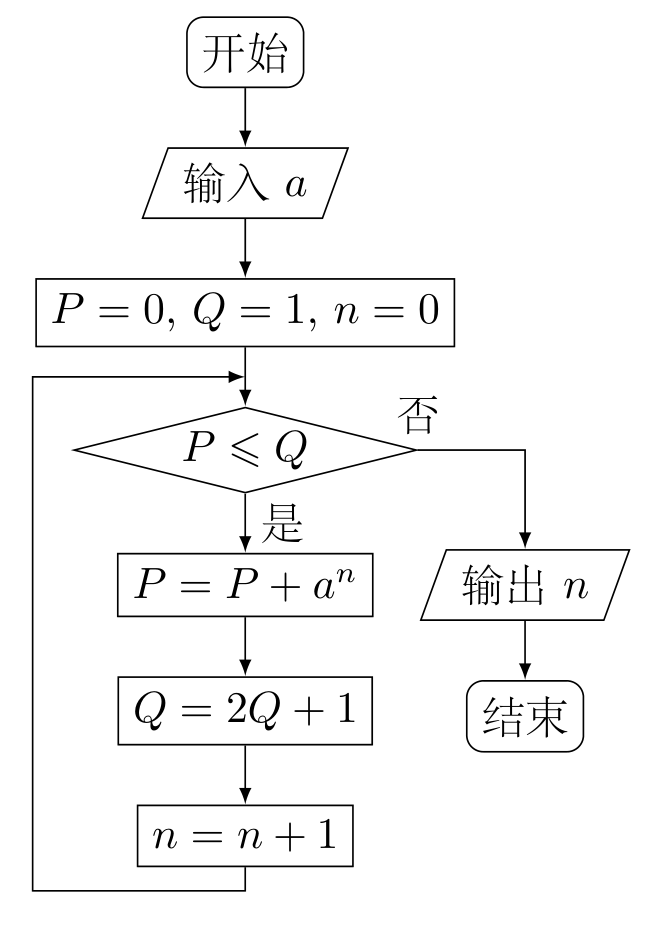
\includegraphics[width=0.55\linewidth]{GaoKao/images/2012/shandong_liberal/q7_fig1.png}
\end{center}

        {\centering\begin{tabular*}{\linewidth}{@{}@{\extracolsep{\fill}}llll@{}}
          \text{A. }2  &  \text{B. }3  &  \text{C. }4  &  \text{D. }5
        \end{tabular*}\par}

        \item 函数 \( y = 2\sin \left(\frac{\pi x}{6} - \frac{\pi}{3}\right) (0 \leqslant x \leqslant 9) \) 的最大值与最小值之和为（\quad）

        {\centering\begin{tabular*}{\linewidth}{@{}@{\extracolsep{\fill}}llll@{}}
          \text{A. }\(2 - \sqrt{3}\)  &  \text{B. }0  &  \text{C. }\(-1\)  &  \text{D. }\(-1 - \sqrt{3}\)
        \end{tabular*}\par}

        \item 圆 \((x + 2)^2 + y^2 = 4\) 与圆 \((x - 2)^2 + (y - 1)^2 = 9\) 的位置关系为（\quad）

        {\centering\begin{tabular*}{\linewidth}{@{}@{\extracolsep{\fill}}llll@{}}
          \text{A. }内切  &  \text{B. }相交  &  \text{C. }外切  &  \text{D. }相离
        \end{tabular*}\par}

        \item 函数 \( f(x) = \frac{\cos 6x}{2^x - 2^{-x}} \) 的图象大致为（\quad）

        {\centering\begin{tabular*}{\linewidth}{@{}@{\extracolsep{\fill}}cccc@{}}
          \text{A. }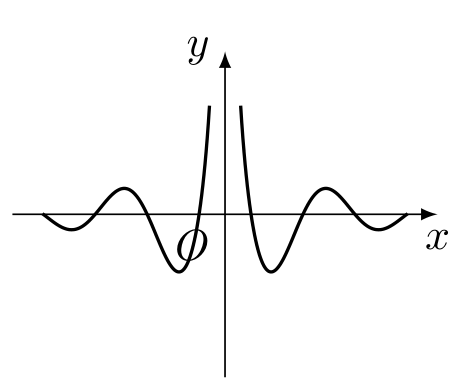
\includegraphics[width=0.15\paperwidth]{GaoKao/images/2012/shandong_liberal/q10_optA.png}  &  \text{B. }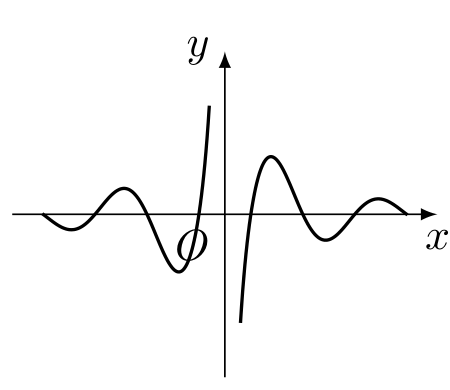
\includegraphics[width=0.15\paperwidth]{GaoKao/images/2012/shandong_liberal/q10_optB.png}  &  \text{C. }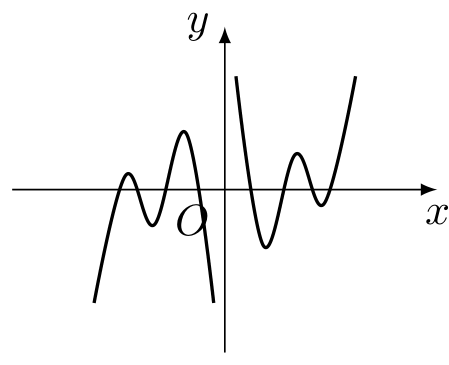
\includegraphics[width=0.15\paperwidth]{GaoKao/images/2012/shandong_liberal/q10_optC.png}  &  \text{D. }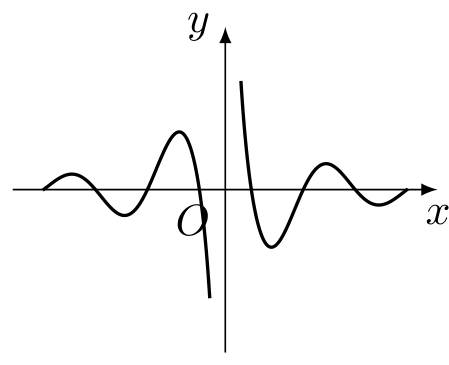
\includegraphics[width=0.15\paperwidth]{GaoKao/images/2012/shandong_liberal/q10_optD.png}
        \end{tabular*}\par}

        \item 已知双曲线 \(C_{1}:\frac{x^{2}}{a^{2}} -\frac{y^{2}}{b^{2}} = 1\) （\(a > 0,b > 0\)）的离心率为2，若抛物线 \(C_2\)：\(x^{2} = 2py\) （\(p > 0\)）的焦点到双曲线 \(C_1\) 的渐近线的距离为2，则抛物线 \(C_2\) 的方程为（\quad）

        {\centering\begin{tabular*}{\linewidth}{@{}@{\extracolsep{\fill}}llll@{}}
          \text{A. }\(x^{2} = \frac{8\sqrt{3}}{3} y\)  &  \text{B. }\(x^{2} = \frac{16\sqrt{3}}{3} y\)  &  \text{C. }\(x^{2} = 8y\)  &  \text{D. }\(x^{2} = 16y\)
        \end{tabular*}\par}

        \item 设函数 \( f(x) = \frac{1}{x} \)，\( g(x) = -x^2 + bx \). 若 \( y = f(x) \) 的图象与 \( y = g(x) \) 的图象有且仅有两个不同的公共点 \(A(x_1, y_1)\)，\(B(x_2, y_2)\)，则下列判断正确的是（\quad）

        {\centering\begin{tabular*}{\linewidth}{@{}@{\extracolsep{\fill}}llll@{}}
          \text{A. }\(x_{1} + x_{2} > 0, y_{1} + y_{2} > 0\)  &  \text{B. }\(x_{1} + x_{2} > 0\)，\(y_{1} + y_{2} < 0\)  &  \text{C. }\(x_{1} + x_{2} < 0\)，\(y_{1} + y_{2} > 0\)  &  \text{D. }\(x_{1} + x_{2} < 0\)，\(y_{1} + y_{2} < 0\)
        \end{tabular*}\par}

    \end{enumerate}

\end{description}

\begin{description}

    \item[二、填空题]

    \begin{enumerate}[leftmargin=5pt]

      \addtocounter{enumi}{+12}

        \item 如图，正方体 \(ABCD - A_{1}B_{1}C_{1}D_{1}\) 的棱长为 \(1\)，\(E\) 为线段 \(B_{1}C\) 上的一点，则三棱锥 \(A - DE D_{1}\) 的体积为\rule[-0.3ex]{3em}{0.4pt}.
\begin{center}
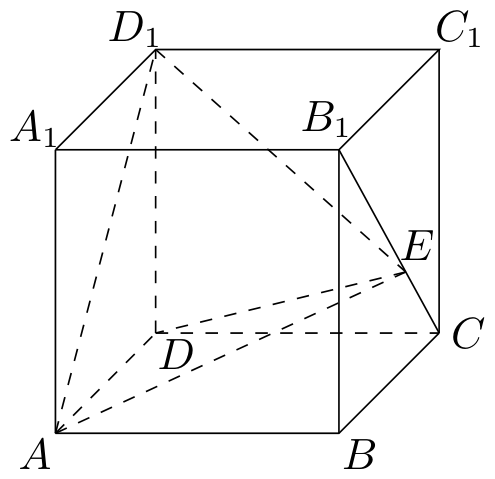
\includegraphics[width=5.0cm]{GaoKao/images/2012/shandong_liberal/q13_fig1.png}
\end{center}

        \item 如图是根据部分城市某年 6 月份的平均气温（单位：\(^{\circ}\mathrm{C}\)）数据得到的样本频率分布直方图，其中平均气温的范围是 \([20.5, 26.5]\)，样本数据的分组为 \([20.5, 21.5)\)，\([21.5, 22.5)\)，\([22.5, 23.5)\)，\([23.5, 24.5)\)，\([24.5, 25.5)\)，\([25.5, 26.5]\).

已知样本中平均气温低于 \(22.5^{\circ}\mathrm{C}\) 的城市个数为 11，则样本中平均气温不低于 \(25.5^{\circ}\mathrm{C}\) 的城市个数为\rule[-0.3ex]{3em}{0.4pt}.

\begin{center}
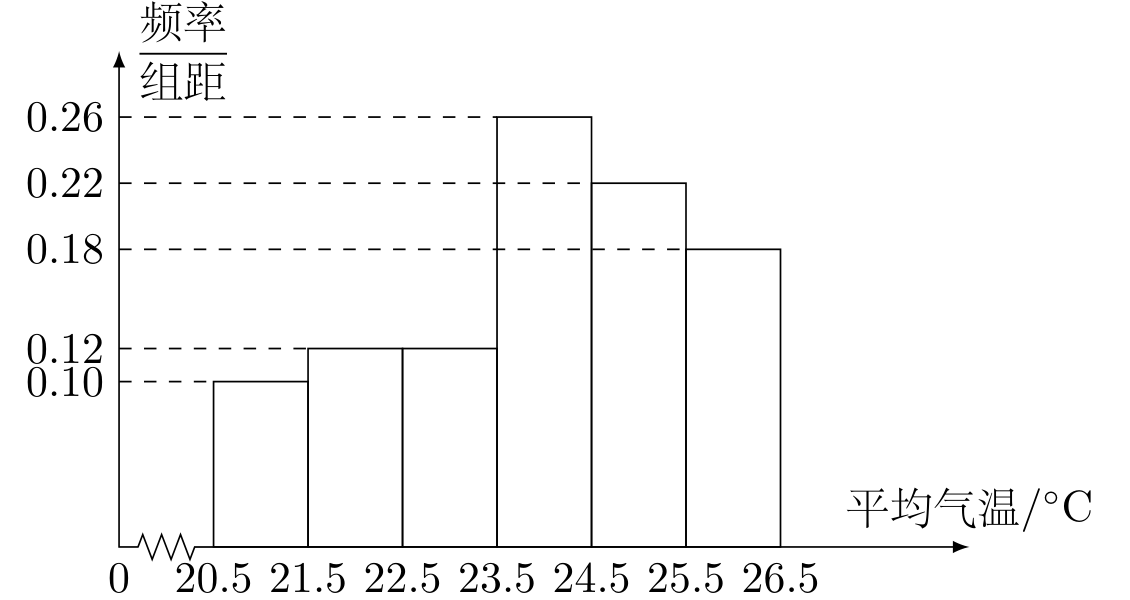
\includegraphics[width=0.75\linewidth]{GaoKao/images/2012/shandong_liberal/q14_fig1.png}
\end{center}

        \item 若函数 \( f(x) = a^x \)（\(a > 0\)，且 \(a \neq 1\)）在 \([-1, 2]\) 上的最大值为 4，最小值为 \( m \)，且函数 \( g(x) = (1 - 4m)\sqrt{x} \) 在 \((0, +\infty)\) 上是增函数，则 \( a = \)\rule[-0.3ex]{3em}{0.4pt}.

        \item 如图，在平面直角坐标系 \(xOy\) 中，一单位圆的圆心初始位置在 \((0,1)\)，此时圆上一点 \(P\) 的位置在 \((0,0)\). 因圆在 \(x\) 轴上沿正向滚动，当圆滚动到圆心位于 \((2,1)\) 时，\(\overrightarrow{OP}\) 的坐标为\rule[-0.3ex]{3em}{0.4pt}.
\begin{center}
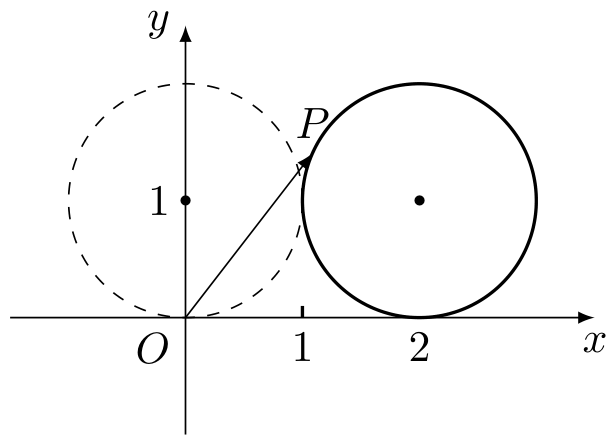
\includegraphics[width=6.0cm]{GaoKao/images/2012/shandong_liberal/q16_fig1.png}
\end{center}

    \end{enumerate}

\end{description}

\begin{description}

    \item[三、解答题]

    \begin{enumerate}[leftmargin=5pt]

      \addtocounter{enumi}{+16}

        \item 在 \(\triangle ABC\) 中，内角 \(A\)，\(B\)，\(C\) 所对的边分别为 \(a\)，\(b\)，\(c\)，已知 \(\sin B (\tan A + \tan C) = \tan A \tan C\).
\begin{enumerate}
\item 求证：\(a\)，\(b\)，\(c\) 成等比数列；
\item 若 \(a = 1\)，\(c = 2\)，求 \(\triangle ABC\) 的面积 \(S\).
\end{enumerate}

        \item 袋中有五张卡片，其中红色卡片三张，标号分别为 \(1\)，\(2\)，\(3\)；蓝色卡片两张，标号分别为 \(1\)，\(2\).
\begin{enumerate}
\item 从以上五张卡片中任取两张，求这两张卡片颜色不同且标号之和小于 4 的概率；
\item 现袋中再放入一张标号为 0 的绿色卡片，从这六张卡片中任取两张，求这两张卡片颜色不同且标号之和小于 4 的概率.
\end{enumerate}

        \item 如图，几何体 \(E - ABCD\) 是四棱锥，\(\triangle ABD\) 为正三角形，\(CB = CD\)，\(EC \perp BD\).
\begin{enumerate}
\item 求证：\(BE = DE\)；
\item 若 \(\angle BCD = 120^{\circ}\)，\(M\) 为线段 \(AE\) 的中点，求证：\(DM \parallel\) 平面 \(BEC\).
\end{enumerate}
\begin{center}
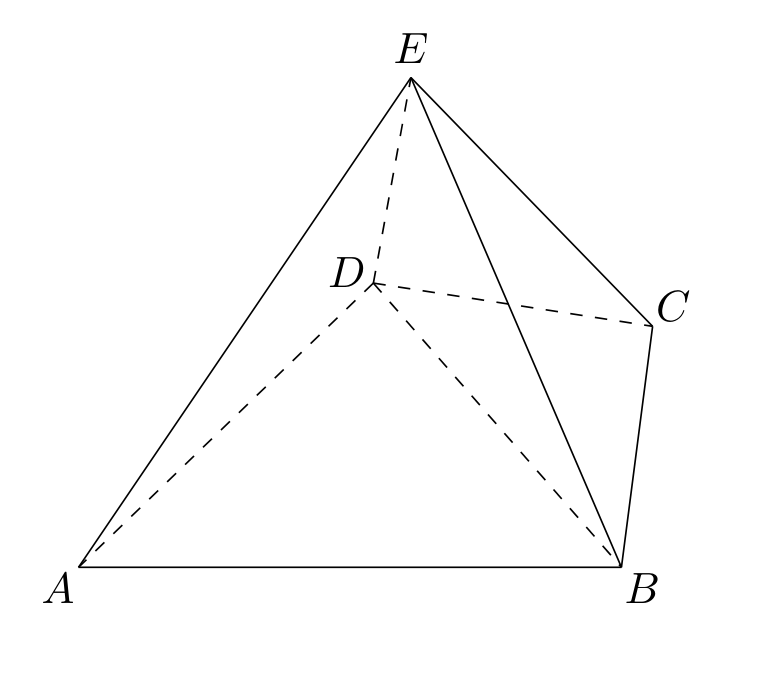
\includegraphics[width=11.0cm]{GaoKao/images/2012/shandong_liberal/q19_fig1.png}
\end{center}

        \item 已知等差数列 \(\{a_{n}\}\) 的前5项和为105，且 \(a_{10} = 2a_{5}\).
\begin{enumerate}
\item 求数列 \(\{a_{n}\}\) 的通项公式；
\item 对任意 \(m \in \mathbb{N}^*\)，将数列 \(\{a_n\}\) 中不大于 \(7^{2m}\) 的项的个数记为 \(b_m\). 求数列 \(\{b_m\}\) 的前 \(m\) 项和 \(S_m\).
\end{enumerate}

        \item 如图，椭圆 \(M: \frac{x^2}{a^2} + \frac{y^2}{b^2} = 1\) （\(a > b > 0\)） 的离心率为 \(\frac{\sqrt{3}}{2}\)，直线 \(x = \pm a\) 和 \(y = \pm b\) 所围成的矩形 \(ABCD\) 的面积为 \(8\).
\begin{enumerate}
\item 求椭圆 \(M\) 的标准方程；
\item 设直线 \(l: y = x + m\) （\(m \in \mathbb{R}\)）与椭圆 \(M\) 有两个不同的交点 \(P\)，\(Q\)，\(l\) 与矩形 \(ABCD\) 有两个不同的交点 \(S\)，\(T\). 求 \(\frac{|PQ|}{|ST|}\) 的最大值及取得最大值时 \(m\) 的值.
\end{enumerate}
\begin{center}
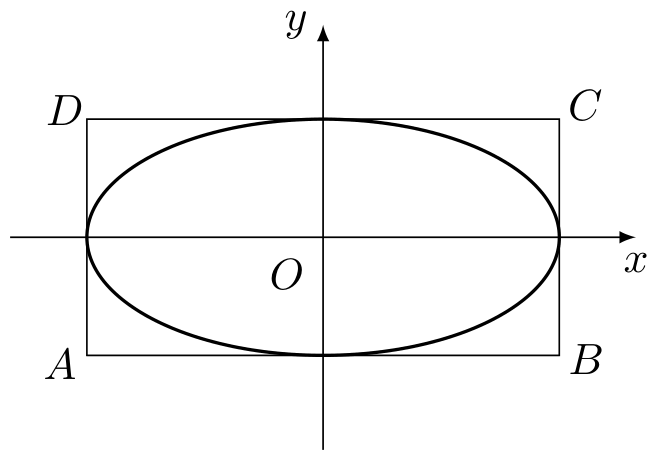
\includegraphics[width=6.3cm]{GaoKao/images/2012/shandong_liberal/q21_fig1.png}
\end{center}

        \item 已知函数 \( f(x) = \frac{\ln x + k}{{\mathrm{e}}^x} \)（\(k\) 为常数，\({\mathrm{e}} = 2.71828 \cdots\) 是自然对数的底数），曲线 \( y = f(x) \) 在点 \((1, f(1))\) 处的切线与 \( x \) 轴平行.
\begin{enumerate}
\item 求 \(k\) 的值；
\item 求 \( f(x) \) 的单调区间；
\item 设 \( g(x) = xf'(x) \)，其中 \( f'(x) \) 为 \( f(x) \) 的导函数. 证明：对任意 \( x > 0 \)，\( g(x) < 1 + {\mathrm{e}}^{-2} \).
\end{enumerate}

    \end{enumerate}

\end{description}


\subsection{2012年陕西卷（理）}\label{gk:2012年陕西卷（理）}

\begin{description}

    \item[一、选择题]

    \begin{enumerate}[leftmargin=5pt]

        \item 集合 \(M = \{x \mid \lg x > 0\}\)，\(N = \{x \mid x^2 \leqslant 4\}\)，则 \(M \cap N =\)（\quad）

        {\centering\begin{tabular*}{\linewidth}{@{}@{\extracolsep{\fill}}llll@{}}
          \text{A. }\((1,2)\)  &  \text{B. }\([1,2)\)  &  \text{C. }\((1,2]\)  &  \text{D. }\([1,2]\)
        \end{tabular*}\par}

        \item 下列函数中，既是奇函数又是增函数的为（\quad）

        {\centering\begin{tabular*}{\linewidth}{@{}@{\extracolsep{\fill}}llll@{}}
          \text{A. }\(y = x + 1\)  &  \text{B. }\( y = -x^3 \)  &  \text{C. }\( y = \frac{1}{x} \)  &  \text{D. }\(y = x|x|\)
        \end{tabular*}\par}

        \item 设 \(a\)，\(b \in \mathbb{R}\)，\(\i\) 是虚数单位，则“\(ab = 0\)”是“复数 \(a + \frac{b}{\i}\) 为纯虚数”的（\quad）

        {\centering\begin{tabular*}{\linewidth}{@{}@{\extracolsep{\fill}}llll@{}}
          \text{A. }充分不必要条件  &  \text{B. }必要不充分条件  &  \text{C. }充分必要条件  &  \text{D. }既不充分也不必要条件
        \end{tabular*}\par}

        \item 已知圆 \(C: x^{2} + y^{2} - 4x = 0\)，\(l\) 是过点 \(P(3,0)\) 的直线，则（\quad）

        {\centering\begin{tabular*}{\linewidth}{@{}@{\extracolsep{\fill}}llll@{}}
          \text{A. }\(l\) 与 \(C\) 相交  &  \text{B. }\(l\) 与 \(C\) 相切  &  \text{C. }\(l\) 与 \(C\) 相离  &  \text{D. }以上三个选项均有可能
        \end{tabular*}\par}

        \item 如图，在空间直角坐标系中有直三棱柱 \(ABC - A_{1}B_{1}C_{1}\)，\(CA = CC_{1} = 2CB\)，则直线 \(BC_{1}\) 与直线 \(AB_{1}\) 夹角的余弦值为（\quad）

\begin{center}
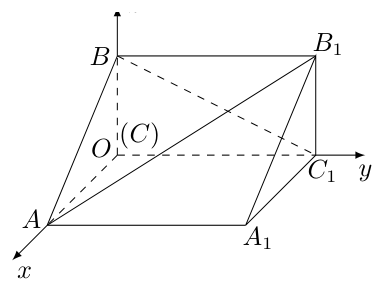
\includegraphics[width=0.34\linewidth]{GaoKao/images/2012/shaanxi_science/q5_fig1.png}
\end{center}

        {\centering\begin{tabular*}{\linewidth}{@{}@{\extracolsep{\fill}}llll@{}}
          \text{A. }\(\frac{\sqrt{5}}{5}\)  &  \text{B. }\( \frac{\sqrt{5}}{3} \)  &  \text{C. }\( \frac{2\sqrt{5}}{5} \)  &  \text{D. }\(\frac{3}{5}\)
        \end{tabular*}\par}

        \item 从甲，乙两个城市分别随机抽取 \(16\text{ 台}\) 自动售货机. 对其销售额进行统计，统计数据用茎叶图表示（如图所示）. 设甲，乙两组数据的平均数分别为 \(\overline{x}_{\text{甲}}\)，\(\overline{x}_{\text{乙}}\)，中位数分别为 \(m_{\text{甲}}\)，\(m_{\text{乙}}\)，则（\quad）

\begin{center}
\begin{tabular}{c|c|c}
甲 & & 乙 \\
\hline
\(8\quad 6\quad 5\) & 0 & \\
\(8\quad 8\quad 4\quad 0\quad 0\) & 1 & \(0\quad 2\quad 8\) \\
\(7\quad 5\quad 2\) & 2 & \(0\quad 2\quad 3\quad 3\quad 7\) \\
\(8\quad 0\quad 0\) & 3 & \(1\quad 2\quad 4\quad 4\quad 8\) \\
\(3\quad 1\) & 4 & \(2\quad 3\quad 8\)
\end{tabular}
\end{center}

        {\centering\begin{tabular*}{\linewidth}{@{}@{\extracolsep{\fill}}llll@{}}
          \text{A. }\(\overline{x}_\text{甲} < \overline{x}_\text{乙}\)，\(m_{\text{甲}} > m_\text{乙}\)  &  \text{B. }\(\overline{x}_\text{甲} < \overline{x}_\text{乙}\)，\(m_{\text{甲}} < m_\text{乙}\)  &  \text{C. }\(\overline{x}_{\text{甲}} > \overline{x}_{\text{乙}}\)，\(m_{\text{甲}} > m_{\text{乙}}\)  &  \text{D. }\(\overline{x}_{\text{甲}} > \overline{x}_{\text{乙}}\)，\(m_{\text{甲}} < m_{\text{乙}}\)
        \end{tabular*}\par}

        \item 设函数 \( f(x) = x{\mathrm{e}}^{x} \)，则（\quad）

        {\centering\begin{tabular*}{\linewidth}{@{}@{\extracolsep{\fill}}llll@{}}
          \text{A. }\(x = 1\) 为 \(f(x)\) 的极大值点  &  \text{B. }\(x = 1\) 为 \(f(x)\) 的极小值点  &  \text{C. }\(x = -1\) 为 \(f(x)\) 的极大值点  &  \text{D. }\(x = -1\) 为 \(f(x)\) 的极小值点
        \end{tabular*}\par}

        \item 两人进行乒乓球比赛，先赢 3 局者获胜，决出胜负为止，则所有可能出现的情形（各人输赢局次的不同视为不同情形）共有（\quad）

        {\centering\begin{tabular*}{\linewidth}{@{}@{\extracolsep{\fill}}llll@{}}
          \text{A. }10 种  &  \text{B. }15 种  &  \text{C. }20 种  &  \text{D. }30 种
        \end{tabular*}\par}

        \item 在 \(\triangle ABC\) 中，角 \(A\)，\(B\)，\(C\) 所对的边长分别为 \(a\)，\(b\)，\(c\)，若 \(a^2 + b^2 = 2c^2\)，则 \(\cos C\) 的最小值为（\quad）

        {\centering\begin{tabular*}{\linewidth}{@{}@{\extracolsep{\fill}}llll@{}}
          \text{A. }\( \frac{\sqrt{3}}{2} \)  &  \text{B. }\( \frac{\sqrt{2}}{2} \)  &  \text{C. }\( \frac{1}{2} \)  &  \text{D. }\(-\frac{1}{2}\)
        \end{tabular*}\par}

        \item 如图所示是用模拟方法估计圆周率 \(\pi\) 值的程序框图，\(P\) 表示估计结果，则图中空白框内应填入（\quad）

\begin{center}
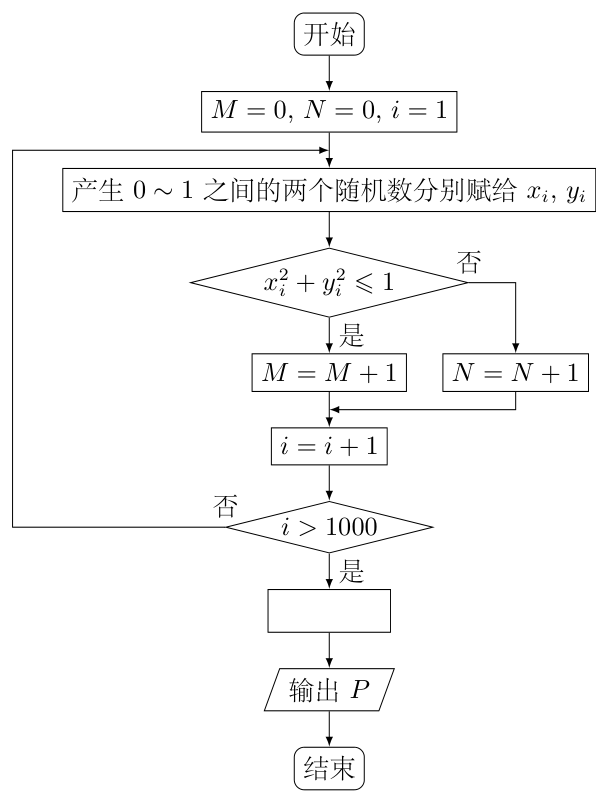
\includegraphics[width=7.2cm]{GaoKao/images/2012/shaanxi_science/q10_fig1.png}
\end{center}

        {\centering\begin{tabular*}{\linewidth}{@{}@{\extracolsep{\fill}}llll@{}}
          \text{A. }\(P = \frac{N}{1000}\)  &  \text{B. }\(P = \frac{4N}{1000}\)  &  \text{C. }\(P = \frac{M}{1000}\)  &  \text{D. }\(P = \frac{4M}{1000}\)
        \end{tabular*}\par}

    \end{enumerate}

\end{description}

\begin{description}

    \item[二、填空题]

    \begin{enumerate}[leftmargin=5pt]

      \addtocounter{enumi}{+10}

        \item 观察下列不等式：\(1 + \frac{1}{2^{2}} < \frac{3}{2}\)，\(1 + \frac{1}{2^{2}} + \frac{1}{3^{2}} < \frac{5}{3}\)，\(1 + \frac{1}{2^{2}} + \frac{1}{3^{2}} + \frac{1}{4^{2}} < \frac{7}{4}\)，照此规律，第五个不等式为\rule[-0.3ex]{3em}{0.4pt}.

        \item \((a + x)^{5}\) 展开式中 \(x^{2}\) 的系数为 10，则实数 \(a\) 的值为\rule[-0.3ex]{3em}{0.4pt}.

        \item 如图是抛物线形拱桥，当水面在 \(l\) 时，拱顶离水面 \(2\text{ 米}\)，水面宽 \(4\text{ 米}\)，水位下降 \(1\text{ 米}\) 后，水面宽\rule[-0.3ex]{3em}{0.4pt}\(\text{米}\).

\begin{center}
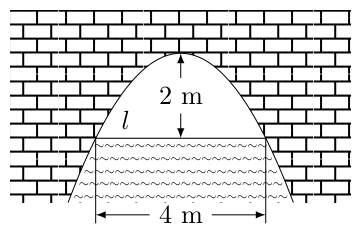
\includegraphics[width=7.4cm]{GaoKao/images/2012/shaanxi_science/q13_fig1.png}
\end{center}

        \item 设函数 \( f(x) = \begin{cases}
\ln x, & x > 0,\\
-2x - 1, & x \leqslant 0,
\end{cases} \) \(D\) 是由 \( x \) 轴和曲线 \( y = f(x) \) 及该曲线在点 \((1,0)\) 处的切线所围成的封闭区域，则 \( z = x - 2y \) 在 \(D\) 上的最大值为\rule[-0.3ex]{3em}{0.4pt}.

    \end{enumerate}

\end{description}

\begin{description}

    \item[三、选做题]

    \begin{enumerate}[leftmargin=5pt]

      \addtocounter{enumi}{+14}

        \item [A]
若存在实数 \(x\) 使 \(\left|x-a\right|+\left|x-1\right|\leqslant 3\) 成立，则实数 \(a\) 的取值范围是\rule[-0.3ex]{3em}{0.4pt}.

        \item \textbf{【选修4-1：几何证明选讲】}

[B]
如图，在圆 \(O\) 中，直径 \(AB\) 与弦 \(CD\) 垂直，垂足为 \(E\)，\(EF \perp DB\)，垂足为 \(F\)，若 \(AB = 6\)，\(AE = 1\)，则 \(DF \cdot DB = \)\rule[-0.3ex]{3em}{0.4pt}.

\begin{center}
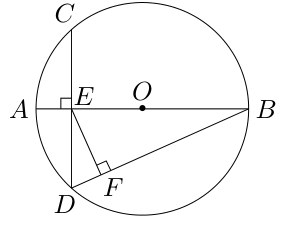
\includegraphics[width=4.3cm]{GaoKao/images/2012/shaanxi_science/q15_fig1.png}
\end{center}

        \item \textbf{【选修4-1：几何证明选讲】}

[C]
直线 \(2\rho\cos \theta = 1\) 与圆 \(\rho = 2\cos \theta\) 相交的弦长为\rule[-0.3ex]{3em}{0.4pt}.

    \end{enumerate}

\end{description}

\begin{description}

    \item[四、解答题]

    \begin{enumerate}[leftmargin=5pt]

      \addtocounter{enumi}{+17}

        \item 函数 \(f(x) = A \sin \left(\omega x - \frac{\pi}{6}\right) + 1\)（\(A > 0\)，\(\omega > 0\)）的最大值为 \(3\)，其图象相邻两条对称轴之间的距离为 \(\frac{\pi}{2}\).

\begin{enumerate}
\item 求函数 \(f(x)\) 的解析式.
\item 设 \(\alpha \in \left(0, \frac{\pi}{2}\right)\)，\(f\left(\frac{\alpha}{2}\right) = 2\)，求 \(\alpha\) 的值.
\end{enumerate}

        \item 设 \(\{a_{n}\}\) 是公比不为 \(1\) 的等比数列，其前 \(n\) 项和为 \(S_{n}\)，且 \(a_{5}\)，\(a_{3}\)，\(a_{4}\) 成等差数列.

\begin{enumerate}
\item 求数列 \(\{a_{n}\}\) 的公比.
\item 证明：对任意 \(k \in \mathbb{N}_+\)，\(S_{k+2}\)，\(S_{k}\)，\(S_{k+1}\) 成等差数列.
\end{enumerate}

        \item \begin{enumerate}
\item 如图，证明命题“\(a\) 是平面 \(\pi\) 内的一条直线，\(b\) 是 \(\pi\) 外的一条直线（\(b\) 不垂直于 \(\pi\)），\(c\) 是直线 \(b\) 在 \(\pi\) 上的投影，若 \(a \perp b\)，则 \(a \perp c\)”为真.
\item 写出上述命题的逆命题，并判断其真假（不需证明）.
\end{enumerate}

\begin{center}
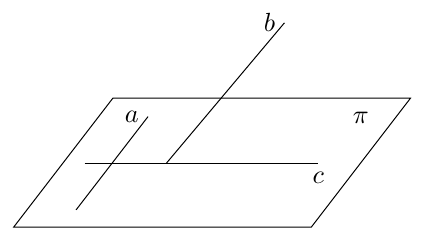
\includegraphics[width=12.4cm]{GaoKao/images/2012/shaanxi_science/q18_fig1.png}
\end{center}

        \item 已知椭圆 \(C_1: \frac{x^2}{4} + y^2 = 1\)，椭圆 \(C_2\) 以 \(C_1\) 的长轴为短轴，且与 \(C_1\) 有相同的离心率.

\begin{enumerate}
\item 求椭圆 \(C_2\) 的方程.
\item 设 \(O\) 为坐标原点，点 \(A\)，\(B\) 分别在椭圆 \(C_1\) 和 \(C_2\) 上，\(\overrightarrow{OB} = 2\overrightarrow{OA}\)，求直线 \(AB\) 的方程.
\end{enumerate}

        \item 某银行柜台设有一个服务窗口，假设顾客办理业务所需的时间互相独立，且都是整数分钟，对以往顾客办理业务所需的时间统计结果如下：

\begin{center}
\begin{tabular}{c|ccccc}
办理业务所需的时间（分） & 1 & 2 & 3 & 4 & 5 \\
\hline
频率 & 0.1 & 0.4 & 0.3 & 0.1 & 0.1
\end{tabular}
\end{center}

从第一个顾客开始办理业务时计时.

\begin{enumerate}
\item 估计第三个顾客恰好等待 \(4\text{ 分钟}\) 开始办理业务的概率.
\item \(X\) 表示至第 \(2\text{ 分钟}\) 末已办理完业务的顾客人数，求 \(X\) 的分布列及数学期望.
\end{enumerate}

        \item 设函数 \(f_{n}(x) = x^{n} + bx + c\)（\(n \in \mathbb{N}_+\)，\(b\)，\(c \in \mathbb{R}\)）.

\begin{enumerate}
\item 设 \(n \geqslant 2\)，\(b = 1\)，\(c = -1\)，证明：\(f_n(x)\) 在区间 \(\left(\frac{1}{2}, 1\right)\) 内存在唯一零点.
\item 设 \(n = 2\)，若对任意 \(x_1\)，\(x_2 \in [-1, 1]\)，有 \(|f_2(x_1) - f_2(x_2)| \leqslant 4\)，求 \(b\) 的取值范围.
\item 在第（1）问的条件下，设 \(x_{n}\) 是 \(f_{n}(x)\) 在 \(\left(\frac{1}{2}, 1\right)\) 内的零点，判断数列 \(x_{2}\)，\(x_{3}\)，\(\cdots\)，\(x_{n}\)，\(\cdots\) 的增减性.
\end{enumerate}

    \end{enumerate}

\end{description}


\subsection{2012年陕西卷（文）}\label{gk:2012年陕西卷（文）}

\begin{description}

    \item[一、选择题]

    \begin{enumerate}[leftmargin=5pt]

        \item 集合 \(M = \{x \mid \lg x > 0\}\)，\(N = \{x \mid x^2 \leqslant 4\}\)，则 \(M \cap N =\)（\quad）

        {\centering\begin{tabular*}{\linewidth}{@{}@{\extracolsep{\fill}}llll@{}}
          \text{A. }\((1,2)\)  &  \text{B. }\([1,2)\)  &  \text{C. }\((1,2]\)  &  \text{D. }\([1,2]\)
        \end{tabular*}\par}

        \item 下列函数中，既是奇函数又是增函数的为（\quad）

        {\centering\begin{tabular*}{\linewidth}{@{}@{\extracolsep{\fill}}llll@{}}
          \text{A. }\(y = x + 1\)  &  \text{B. }\(y = -x^3\)  &  \text{C. }\(y = \frac{1}{x}\)  &  \text{D. }\(y = x|x|\)
        \end{tabular*}\par}

        \item 对某商店一个月内每天的顾客人数进行了统计，得到样本的茎叶图如图所示. 则该样本的中位数，众数，极差分别是（\quad）

\begin{center}
\begin{tabular}{c|l}
\(1\) & \(2\quad 5\) \\
\(2\) & \(0\quad 2\quad 3\quad 3\) \\
\(3\) & \(1\quad 2\quad 4\quad 4\quad 8\quad 9\) \\
\(4\) & \(5\quad 5\quad 5\quad 7\quad 7\quad 8\quad 8\quad 9\) \\
\(5\) & \(0\quad 0\quad 1\quad 1\quad 4\quad 7\quad 9\) \\
\(6\) & \(1\quad 7\quad 8\)
\end{tabular}
\end{center}

        {\centering\begin{tabular*}{\linewidth}{@{}@{\extracolsep{\fill}}llll@{}}
          \text{A. }\(46\)，\(45\)，\(56\)  &  \text{B. }\(46\)，\(45\)，\(53\)  &  \text{C. }\(47\)，\(45\)，\(56\)  &  \text{D. }\(45\)，\(47\)，\(53\)
        \end{tabular*}\par}

        \item 设 \(a,b \in \mathbb{R}\)，\(\i\) 是虚数单位，则“\(ab = 0\)”是“复数 \(a + \frac{b}{\i}\) 为纯虚数”的（\quad）

        {\centering\begin{tabular*}{\linewidth}{@{}@{\extracolsep{\fill}}llll@{}}
          \text{A. }充分不必要条件  &  \text{B. }必要不充分条件  &  \text{C. }充分必要条件  &  \text{D. }既不充分也不必要条件
        \end{tabular*}\par}

        \item 如图所示是计算某年级 \(500\text{ 名}\) 学生期末考试（满分为 \(100\text{ 分}\)）及格率 \(q\) 的程序框图，则图中空白框内应填入（\quad）

\begin{minipage}{\linewidth}
\centering
\begin{center}
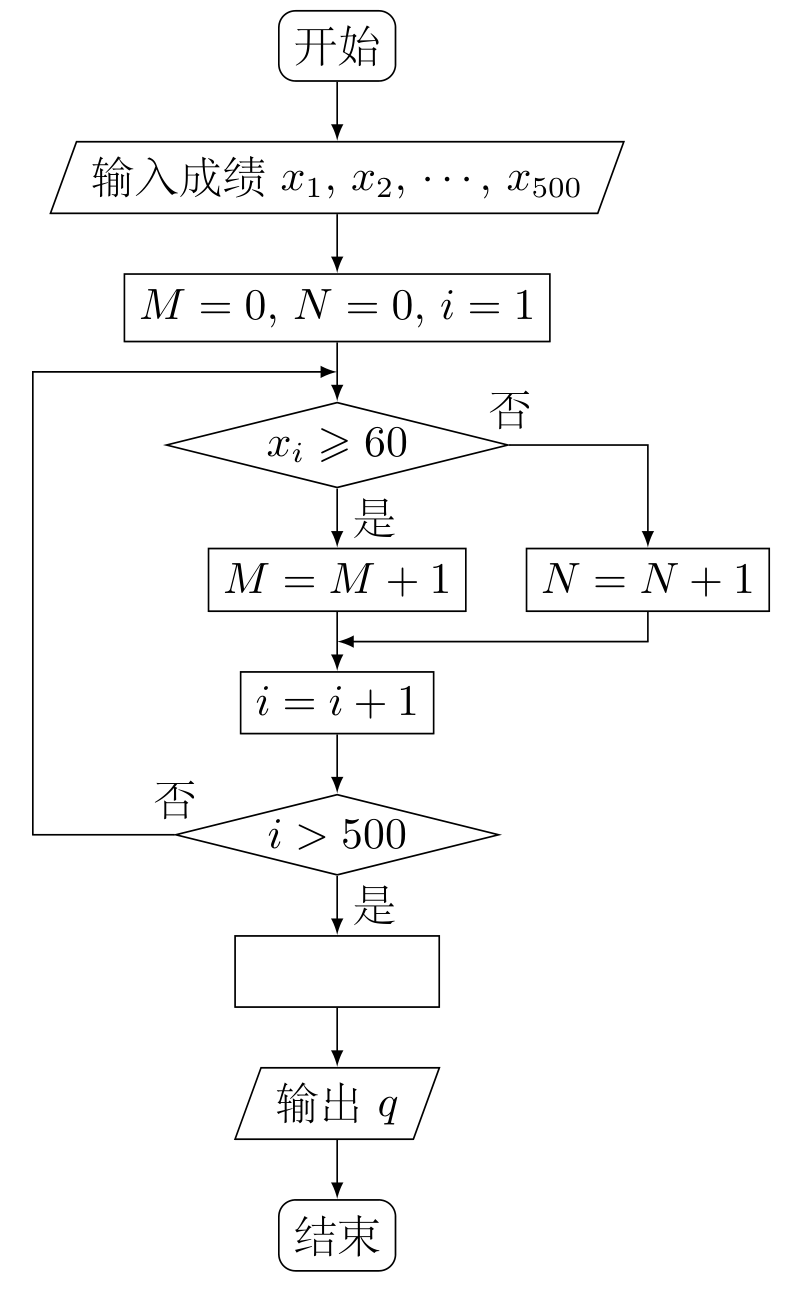
\includegraphics[width=0.46\linewidth]{GaoKao/images/2012/shaanxi_liberal/q5_fig1.png}
\end{center}
\end{minipage}

        {\centering\begin{tabular*}{\linewidth}{@{}@{\extracolsep{\fill}}llll@{}}
          \text{A. }\(q = \frac{N}{M}\)  &  \text{B. }\(q = \frac{M}{N}\)  &  \text{C. }\(q = \frac{N}{M + N}\)  &  \text{D. }\(q = \frac{M}{M + N}\)
        \end{tabular*}\par}

        \item 已知圆 \(C: x^2 + y^2 - 4x = 0\)，\(l\) 是过点 \(P(3,0)\) 的直线，则（\quad）

        {\centering\begin{tabular*}{\linewidth}{@{}@{\extracolsep{\fill}}llll@{}}
          \text{A. }\(l\) 与 \(C\) 相交  &  \text{B. }\(l\) 与 \(C\) 相切  &  \text{C. }\(l\) 与 \(C\) 相离  &  \text{D. }以上三个选项均有可能
        \end{tabular*}\par}

        \item 设向量 \(\bm{a} = (1, \cos \theta)\) 与 \(\bm{b} = (-1, 2 \cos \theta)\) 垂直，则 \(\cos 2\theta\) 等于（\quad）

        {\centering\begin{tabular*}{\linewidth}{@{}@{\extracolsep{\fill}}llll@{}}
          \text{A. }\(\frac{\sqrt{2}}{2}\)  &  \text{B. }\(\frac{1}{2}\)  &  \text{C. }0  &  \text{D. }\(-1\)
        \end{tabular*}\par}

        \item 将正方体（如图 1 所示）截去两个三棱锥，得到图 2 所示的几何体，则该几何体的左视图为（\quad）

\begin{minipage}{\linewidth}
\centering
\begin{center}
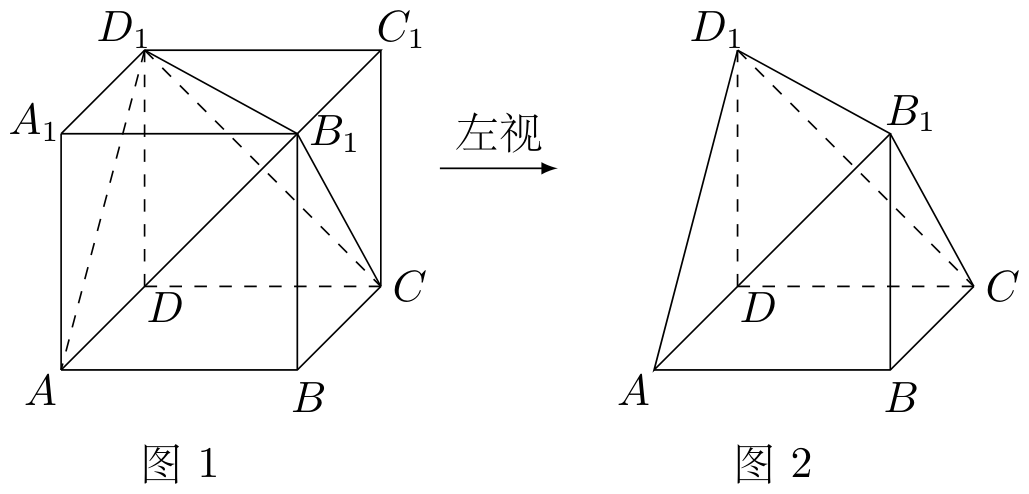
\includegraphics[width=9.7cm]{GaoKao/images/2012/shaanxi_liberal/q8_fig1.png}
\end{center}
\end{minipage}

        {\centering\begin{tabular*}{\linewidth}{@{}@{\extracolsep{\fill}}cccc@{}}
          \text{A. }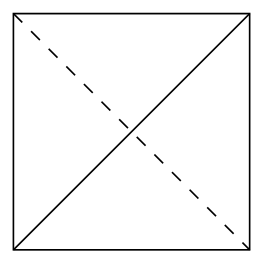
\includegraphics[width=0.15\paperwidth]{GaoKao/images/2012/shaanxi_liberal/q8_optA.png}  &  \text{B. }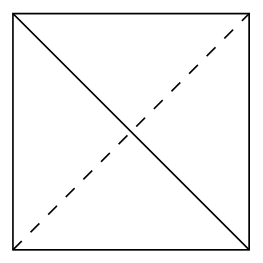
\includegraphics[width=0.15\paperwidth]{GaoKao/images/2012/shaanxi_liberal/q8_optB.png}  &  \text{C. }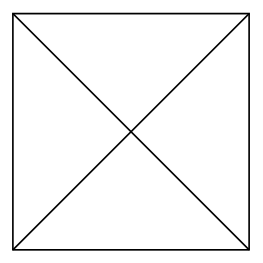
\includegraphics[width=0.15\paperwidth]{GaoKao/images/2012/shaanxi_liberal/q8_optC.png}  &  \text{D. }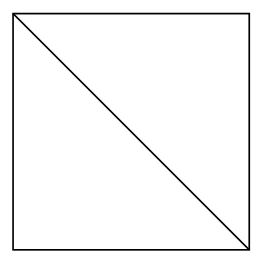
\includegraphics[width=0.15\paperwidth]{GaoKao/images/2012/shaanxi_liberal/q8_optD.png}
        \end{tabular*}\par}

        \item 设函数 \(f(x) = \frac{2}{x} + \ln x\)，则（\quad）

        {\centering\begin{tabular*}{\linewidth}{@{}@{\extracolsep{\fill}}llll@{}}
          \text{A. }\(x = \frac{1}{2}\) 为 \(f(x)\) 的极大值点  &  \text{B. }\(x = \frac{1}{2}\) 为 \(f(x)\) 的极小值点  &  \text{C. }\(x = 2\) 为 \(f(x)\) 的极大值点  &  \text{D. }\(x = 2\) 为 \(f(x)\) 的极小值点
        \end{tabular*}\par}

        \item 小王从甲地到乙地的往返时速分别为 \(a\) 和 \(b\)（\(a < b\)），其全程的平均时速为 \(v\)，则（\quad）

        {\centering\begin{tabular*}{\linewidth}{@{}@{\extracolsep{\fill}}llll@{}}
          \text{A. }\(a < v < \sqrt{ab}\)  &  \text{B. }\(v = \sqrt{ab}\)  &  \text{C. }\(\sqrt{ab} < v < \frac{a + b}{2}\)  &  \text{D. }\(v = \frac{a + b}{2}\)
        \end{tabular*}\par}

    \end{enumerate}

\end{description}

\begin{description}

    \item[二、填空题]

    \begin{enumerate}[leftmargin=5pt]

      \addtocounter{enumi}{+10}

        \item 设函数 \(f(x) = \begin{cases}
\sqrt{x}, & x \geqslant 0,\\
\left(\frac{1}{2}\right)^x, & x < 0.
\end{cases}\) 则 \(f\left(f(-4)\right) = \)\rule[-0.3ex]{3em}{0.4pt}.

        \item 观察下列不等式：\(1 + \frac{1}{2^2} < \frac{3}{2}\)，\(1 + \frac{1}{2^2} + \frac{1}{3^2} < \frac{5}{3}\)，\(1 + \frac{1}{2^2} + \frac{1}{3^2} + \frac{1}{4^2} < \frac{7}{4}\). 照此规律，第五个不等式为\rule[-0.3ex]{3em}{0.4pt}.

        \item 在 \(\triangle ABC\) 中，角 \(A\)，\(B\)，\(C\) 所对应的边长分别为 \(a\)，\(b\)，\(c\)，若 \(a = 2\)，\(B = \frac{\pi}{6}\)，\(c = 2\sqrt{3}\)，则 \(b = \)\rule[-0.3ex]{3em}{0.4pt}.

        \item 如图是抛物线形拱桥，当水面在 \(l\) 时，拱顶离水面 \(2\text{ 米}\)，水面宽 \(4\text{ 米}\)，水位下降 \(1\text{ 米}\) 后，水面宽\rule[-0.3ex]{3em}{0.4pt}\(\text{米}\).

\begin{minipage}{\linewidth}
\centering
\begin{center}
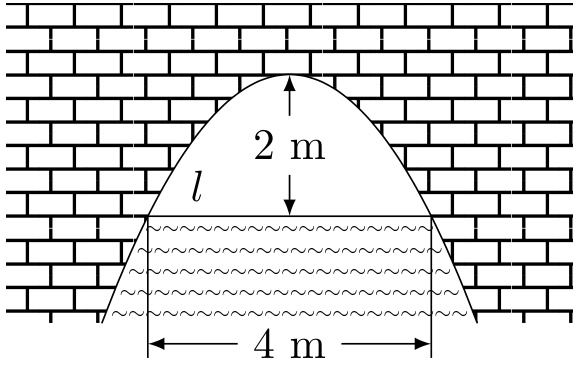
\includegraphics[width=13.6cm]{GaoKao/images/2012/shaanxi_liberal/q14_fig1.png}
\end{center}
\end{minipage}

    \end{enumerate}

\end{description}

\begin{description}

    \item[三、选做题]

    \begin{enumerate}[leftmargin=5pt]

      \addtocounter{enumi}{+14}

        \item [A]
若存在实数 \(x\) 使 \( |x - a| + |x - 1| \leqslant 3 \) 成立，则实数 \(a\) 的取值范围是\rule[-0.3ex]{3em}{0.4pt}.

        \item \textbf{【选修4-1：几何证明选讲】}

[B]
如图，在圆 \(O\) 中，直径 \(AB\) 与弦 \(CD\) 垂直，垂足为 \(E\)，\(EF \perp DB\)，垂足为 \(F\)，若 \(AB = 6\)，\(AE = 1\)，则 \(DF \cdot DB = \)\rule[-0.3ex]{3em}{0.4pt}.

\begin{minipage}{\linewidth}
\centering
\begin{center}
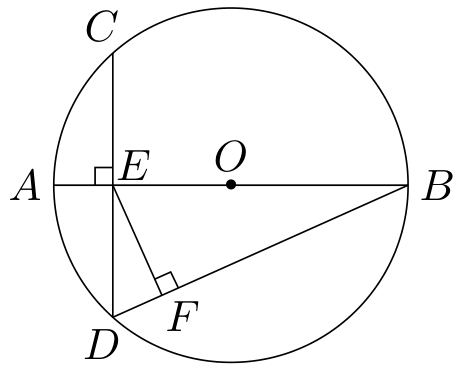
\includegraphics[width=5.4cm]{GaoKao/images/2012/shaanxi_liberal/q15_fig1.png}
\end{center}
\end{minipage}

        \item \textbf{【选修4-1：几何证明选讲】}

[C]
直线 \(2\rho \cos \theta = 1\) 与圆 \(\rho = 2\cos \theta\) 相交的弦长为\rule[-0.3ex]{3em}{0.4pt}.

    \end{enumerate}

\end{description}

\begin{description}

    \item[四、解答题]

    \begin{enumerate}[leftmargin=5pt]

      \addtocounter{enumi}{+17}

        \item 已知等比数列 \(\{a_n\}\) 的公比为 \(q = -\frac{1}{2}\).

\begin{enumerate}
\item 若 \(a_3 = \frac{1}{4}\)，求数列 \(\{a_n\}\) 的前 \(n\) 项和；
\item 证明：对任意 \(k \in \mathbb{N}_+\)，\(a_k\)，\(a_{k+2}\)，\(a_{k+1}\) 成等差数列.
\end{enumerate}

        \item 函数 \(f(x) = A \sin \left(\omega x - \frac{\pi}{6}\right) + 1\)（\(A > 0\)，\(\omega > 0\)）的最大值为 \(3\)，其图象相邻两条对称轴之间的距离为 \(\frac{\pi}{2}\).

\begin{enumerate}
\item 求函数 \(f(x)\) 的解析式；
\item 设 \(\alpha \in \left(0, \frac{\pi}{2}\right)\)，\(f\left(\frac{\alpha}{2}\right) = 2\)，求 \(\alpha\) 的值.
\end{enumerate}

        \item 直三棱柱 \(ABC - A_1B_1C_1\) 中，\(AB = AA_1\)，\(\angle CAB = \frac{\pi}{2}\).

\begin{enumerate}
\item 证明：\(CB_1 \perp BA_1\)；
\item 已知 \(AB = 2\)，\(BC = \sqrt{5}\)，求三棱锥 \(C_1 - ABA_1\) 的体积.
\end{enumerate}

\begin{minipage}{\linewidth}
\centering
\begin{center}
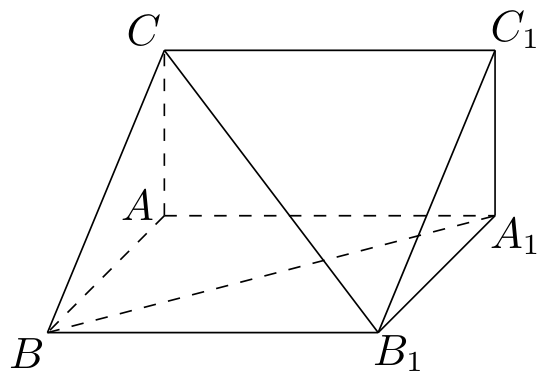
\includegraphics[width=5.5cm]{GaoKao/images/2012/shaanxi_liberal/q18_fig1.png}
\end{center}
\end{minipage}

        \item 假设甲乙两种品牌的同类产品在某地区市场上销售量相等，为了解他们的使用寿命，现从两种品牌的产品中分别随机抽取 \(100\text{ 个}\) 进行测试，结果统计如下：

\begin{enumerate}
\item 估计甲品牌产品寿命小于 \(200\text{ 小时}\) 的概率；
\item 这两种品牌产品中，某个产品已使用了 \(200\text{ 小时}\)，试估计该产品是甲品牌的概率.
\end{enumerate}

\begin{minipage}{\linewidth}
\centering
\begin{center}
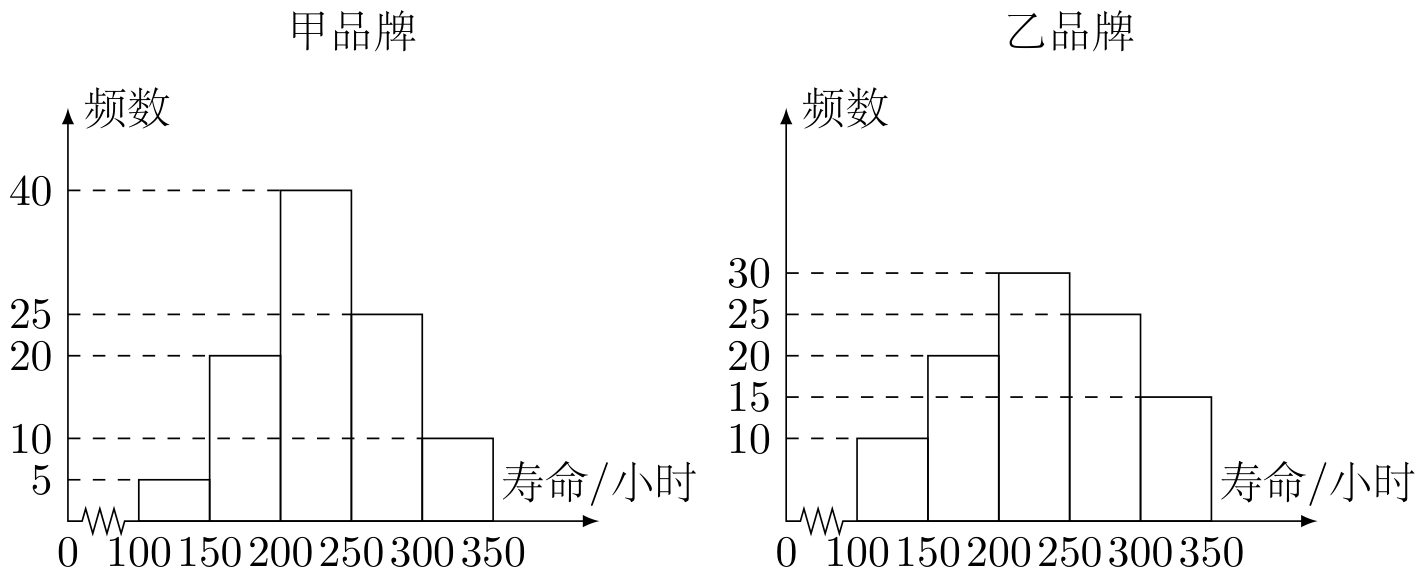
\includegraphics[width=13.7cm]{GaoKao/images/2012/shaanxi_liberal/q19_fig1.png}
\end{center}
\end{minipage}

        \item 已知椭圆 \(C_1: \frac{x^2}{4} + y^2 = 1\)，椭圆 \(C_2\) 以 \(C_1\) 的长轴为短轴，且与 \(C_1\) 有相同的离心率.

\begin{enumerate}
\item 求椭圆 \(C_2\) 的方程；
\item 设 \(O\) 为坐标原点，点 \(A\)，\(B\) 分别在椭圆 \(C_1\) 和 \(C_2\) 上，\(\overrightarrow{OB} = 2\overrightarrow{OA}\)，求直线 \(AB\) 的方程.
\end{enumerate}

        \item 设函数 \(f_n(x) = x^n + bx + c\)（\(n \in \mathbb{N}_+\)，\(b\)，\(c \in \mathbb{R}\)）.

\begin{enumerate}
\item 设 \(n \geqslant 2\)，\(b = 1\)，\(c = -1\)，证明：\(f_n(x)\) 在区间 \(\left(\frac{1}{2}, 1\right)\) 内存在唯一零点；
\item 设 \(n\) 为偶数，\(|f_n(-1)| \leqslant 1\)，\(|f_n(1)| \leqslant 1\)，求 \(b + 3c\) 的最小值和最大值；
\item 设 \(n = 2\)，若对任意 \(x_1\)，\(x_2 \in [-1, 1]\)，有 \(|f_2(x_1) - f_2(x_2)| \leqslant 4\)，求 \(b\) 的取值范围.
\end{enumerate}

    \end{enumerate}

\end{description}


\subsection{2012年天津卷（理）}\label{gk:2012年天津卷（理）}

\begin{description}

    \item[一、选择题]

    \begin{enumerate}[leftmargin=5pt]

        \item \(i\) 是虚数单位，复数 \(\frac{7-\i}{3+\i}=\)（\quad）

        {\centering\begin{tabular*}{\linewidth}{@{}@{\extracolsep{\fill}}llll@{}}
          \text{A. }\(2 + \i\)  &  \text{B. }\(2 - \i\)  &  \text{C. }\(-2 + \i\)  &  \text{D. }\(-2 - \i\)
        \end{tabular*}\par}

        \item 设 \(\varphi \in \mathbb{R}\)，则“\(\varphi = 0\)”是“\(f(x) = \cos (x + \varphi)\)（\(x \in \mathbb{R}\)）为偶函数”的（\quad）

        {\centering\begin{tabular*}{\linewidth}{@{}@{\extracolsep{\fill}}llll@{}}
          \text{A. }充分而不必要条件  &  \text{B. }必要而不充分条件  &  \text{C. }充分必要条件  &  \text{D. }既不充分也不必要条件
        \end{tabular*}\par}

        \item 阅读如图所示的程序框图，运行相应的程序，当输入 \(x\) 的值为 \(-25\) 时，输出 \(x\) 的值为（\quad）

\begin{center}
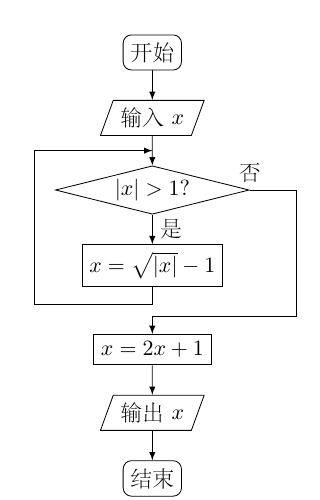
\includegraphics[width=0.42\linewidth]{GaoKao/images/2012/tianjin_science/q3_fig1.png}
\end{center}

        {\centering\begin{tabular*}{\linewidth}{@{}@{\extracolsep{\fill}}llll@{}}
          \text{A. }\(-1\)  &  \text{B. }1  &  \text{C. }3  &  \text{D. }9
        \end{tabular*}\par}

        \item 函数 \( f(x) = 2^x + x^3 - 2 \) 在区间 \((0,1)\) 内的零点个数是（\quad）

        {\centering\begin{tabular*}{\linewidth}{@{}@{\extracolsep{\fill}}llll@{}}
          \text{A. }0  &  \text{B. }1  &  \text{C. }2  &  \text{D. }3
        \end{tabular*}\par}

        \item 在 \(\left(2x^{2} - \frac{1}{x}\right)^{5}\) 的二项展开式中，\(x\) 的系数为（\quad）

        {\centering\begin{tabular*}{\linewidth}{@{}@{\extracolsep{\fill}}llll@{}}
          \text{A. }10  &  \text{B. }\(-10\)  &  \text{C. }40  &  \text{D. }\(-40\)
        \end{tabular*}\par}

        \item 在 \(\triangle ABC\) 中，内角 \(A\)，\(B\)，\(C\) 所对的边分别是 \(a\)，\(b\)，\(c\)，已知 \(8b = 5c\)，\(C = 2B\)，则 \(\cos C =\)（\quad）

        {\centering\begin{tabular*}{\linewidth}{@{}@{\extracolsep{\fill}}llll@{}}
          \text{A. }\(\frac{7}{25}\)  &  \text{B. }\( -\frac{7}{25} \)  &  \text{C. }\(\pm\frac{7}{25}\)  &  \text{D. }\(\frac{24}{25}\)
        \end{tabular*}\par}

        \item 已知 \(\triangle ABC\) 为等边三角形，\(AB = 2\)，设点 \(P\)，\(Q\) 满足 \(\overrightarrow{AP} = \lambda \overrightarrow{AB}\)，\(\overrightarrow{AQ} = (1 - \lambda) \overrightarrow{AC}\)，\(\lambda \in \mathbb{R}\)，若 \(\overrightarrow{BQ} \cdot \overrightarrow{CP} = -\frac{3}{2}\)，则 \(\lambda =\)（\quad）

        {\centering\begin{tabular*}{\linewidth}{@{}@{\extracolsep{\fill}}llll@{}}
          \text{A. }\( \frac{1}{2} \)  &  \text{B. }\( \frac{1 \pm \sqrt{2}}{2} \)  &  \text{C. }\(\frac{1 \pm \sqrt{10}}{2}\)  &  \text{D. }\(\frac{-3 \pm 2\sqrt{2}}{2}\)
        \end{tabular*}\par}

        \item 设 \(m\)，\(n \in \mathbb{R}\)，若直线 \((m + 1)x + (n + 1)y - 2 = 0\) 与圆 \((x - 1)^2 + (y - 1)^2 = 1\) 相切，则 \(m + n\) 的取值范围是（\quad）

        {\centering\begin{tabular*}{\linewidth}{@{}@{\extracolsep{\fill}}llll@{}}
          \text{A. }\([1 - \sqrt{3}, 1 + \sqrt{3}]\)  &  \text{B. }\((-\infty, 1 - \sqrt{3}] \cup [1 + \sqrt{3}, +\infty)\)  &  \text{C. }\([2 - 2\sqrt{2}, 2 + 2\sqrt{2}]\)  &  \text{D. }\((-\infty, 2 - 2\sqrt{2}] \cup [2 + 2\sqrt{2}, +\infty)\)
        \end{tabular*}\par}

    \end{enumerate}

\end{description}

\begin{description}

    \item[二、填空题]

    \begin{enumerate}[leftmargin=5pt]

      \addtocounter{enumi}{+8}

        \item 某地区有小学 150 所，中学 75 所，大学 25 所. 现采用分层抽样的方法从这些学校中抽取 30 所学校对学生进行视力调查，应从小学中抽取\rule[-0.3ex]{3em}{0.4pt} 所学校，中学中抽取\rule[-0.3ex]{3em}{0.4pt} 所学校.

        \item 一个几何体的三视图如图所示（单位：\(\mathrm{m}\)），则该几何体的体积为\rule[-0.3ex]{3em}{0.4pt}\(\mathrm{m}^3\).

\begin{center}
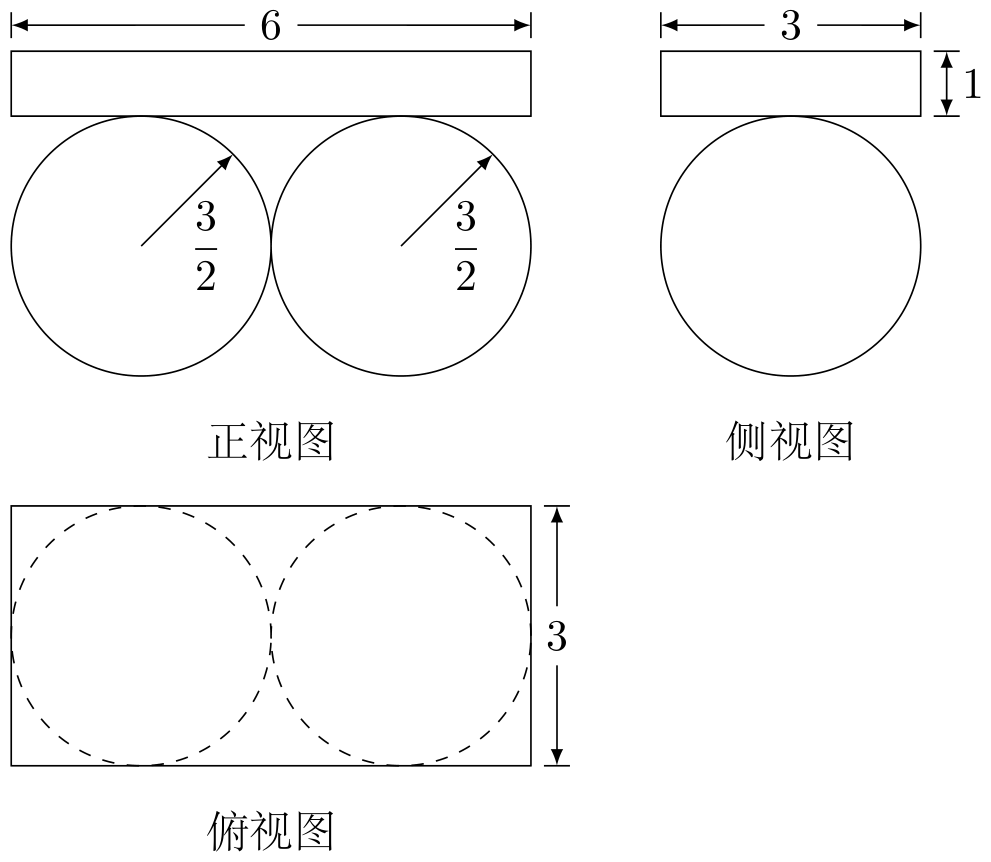
\includegraphics[width=9.7cm]{GaoKao/images/2012/tianjin_science/q10_fig1.png}
\end{center}

        \item 已知集合 \(A = \{x \in \mathbb{R} \mid |x + 2| < 3\}\)，集合 \(B = \{x \in \mathbb{R} \mid (x - m)(x - 2) < 0\}\)，且 \(A \cap B = (-1, n)\)，则 \(m =\rule[-0.3ex]{3em}{0.4pt}\)，\(n =\rule[-0.3ex]{3em}{0.4pt}\).

        \item 已知抛物线的参数方程为 \(\begin{cases}
x = 2pt^2,\\
y = 2pt,
\end{cases}\)（\(t\) 为参数），其中 \(p > 0\)，焦点为 \(F\)，准线为 \(l\)，过抛物线上一点 \(M\) 作 \(l\) 的垂线，垂足为 \(E\)，若 \(|EF| = |MF|\)，点 \(M\) 的横坐标是 3，则 \(p = \)\rule[-0.3ex]{3em}{0.4pt}.

        \item 如图，已知 \(AB\) 和 \(AC\) 是圆的两条弦，过点 \(B\) 作圆的切线与 \(AC\) 的延长线相交于点 \(D\). 过点 \(C\) 作 \(BD\) 的平行线与圆相交于点 \(E\)，与 \(AB\) 相交于点 \(F\)，\(AF = 3\)，\(FB = 1\)，\(EF = \frac{3}{2}\)，则线段 \(CD\) 的长为\rule[-0.3ex]{3em}{0.4pt}.

\begin{center}
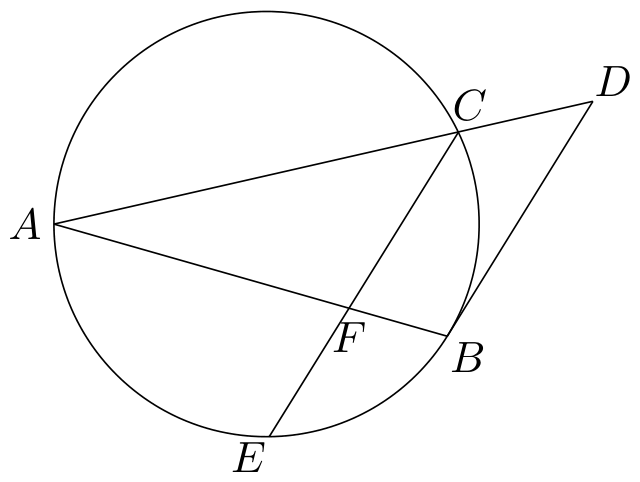
\includegraphics[width=7.9cm]{GaoKao/images/2012/tianjin_science/q13_fig1.png}
\end{center}

        \item 已知函数 \( y = \frac{|x^2 - 1|}{x - 1} \) 的图象与函数 \( y = kx - 2 \) 的图象恰有两个交点，则实数 \( k \) 的取值范围是\rule[-0.3ex]{3em}{0.4pt}.

    \end{enumerate}

\end{description}

\begin{description}

    \item[三、解答题]

    \begin{enumerate}[leftmargin=5pt]

      \addtocounter{enumi}{+14}

        \item 已知函数 \(f(x) = \sin \left(2x + \frac{\pi}{3}\right) + \sin \left(2x - \frac{\pi}{3}\right) + 2\cos^2 x - 1\)，\(x \in \mathbb{R}\).

\begin{enumerate}
\item 求函数 \( f(x) \) 的最小正周期；
\item 求函数 \( f(x) \) 在区间 \( \left[-\frac{\pi}{4}, \frac{\pi}{4}\right] \) 上的最大值和最小值.
\end{enumerate}

        \item 有4个人去参加某娱乐活动，该活动有甲，乙两个游戏可供参加者选择. 为增加趣味性，约定：每个人通过掷一枚质地均匀的骰子决定自己去参加哪个游戏，掷出点数为1或2的人去参加甲游戏，掷出点数大于2的人去参加乙游戏.

\begin{enumerate}
\item 求这 4 个人中恰有 2 人去参加甲游戏的概率；
\item 求这 4 个人中去参加甲游戏的人数大于去参加乙游戏的人数的概率；
\item 用 \(X\)，\(Y\) 分别表示这 4 个人中去参加甲，乙游戏的人数，记 \( \xi = |X - Y| \)，求随机变量 \( \xi \) 的分布列与数学期望 \( E(\xi) \).
\end{enumerate}

        \item 如图，在四棱锥 \(P - ABCD\) 中，\(PA \perp\) 平面 \(ABCD\)，\(AC \perp AD\)，\(AB \perp BC\)，\(\angle BAC = 45^{\circ}\)，\(PA = AD = 2\)，\(AC = 1\).

\begin{enumerate}
\item 证明 \(PC \perp AD\)；
\item 求二面角 \(A - PC - D\) 的正弦值；
\item 设 \(E\) 为棱 \(PA\) 上的点，满足异面直线 \(BE\) 与 \(CD\) 所成的角为 \(30^{\circ}\)，求 \(AE\) 的长.
\end{enumerate}
\begin{center}
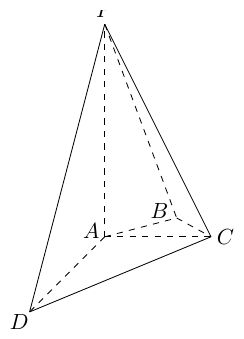
\includegraphics[width=6.7cm]{GaoKao/images/2012/tianjin_science/q17_fig1.png}
\end{center}

        \item 已知 \(\{a_{n}\}\) 是等差数列，其前 \(n\) 项和为 \(S_{n}\)，\(\{b_{n}\}\) 是等比数列，且 \(a_{1} = b_{1} = 2\)，\(a_{4} + b_{4} = 27\)，\(S_{4} - b_{4} = 10\).

\begin{enumerate}
\item 求数列 \( \{a_{n}\} \) 与 \( \{b_{n}\} \) 的通项公式；
\item 记 \(T_{n} = a_{n}b_{1} + a_{n - 1}b_{2} + \dots +a_{1}b_{n}\)，\(n \in \mathbf{N}^{*}\)，证明 \(T_{n} + 12 = -2a_{n} + 10b_{n}\) （\(n \in \mathbf{N}^{*}\)）.
\end{enumerate}

        \item 设椭圆 \(\frac{x^2}{a^2} + \frac{y^2}{b^2} = 1\)（\(a > b > 0\)）的左，右顶点分别为 \(A\)，\(B\)，点 \(P\) 在椭圆上且异于 \(A\)，\(B\) 两点，点 \(O\) 为坐标原点.

\begin{enumerate}
\item 若直线 \(AP\) 与 \(BP\) 的斜率之积为 \(-\frac{1}{2}\)，求椭圆的离心率；
\item 若 \( \left|AP\right|=\left|OA\right| \)，证明直线 \(OP\) 的斜率 \(k\) 满足 \( \left|k\right|>\sqrt{3} \).
\end{enumerate}

        \item 已知函数 \( f(x) = x - \ln (x + a) \) 的最小值为 0，其中 \( a > 0 \).

\begin{enumerate}
\item 求 \(a\) 的值；
\item 若对任意的 \(x \in [0, +\infty)\)，有 \(f(x) \leqslant kx^2\) 成立. 求实数 \(k\) 的最小值；
\item 证明： \(\sum_{i=1}^{n} \frac{2}{2i-1} - \ln(2n+1) < 2\)（\(n \in \mathbf{N}^*\)）.
\end{enumerate}

    \end{enumerate}

\end{description}


\subsection{2012年天津卷（文）}\label{gk:2012年天津卷（文）}

\begin{description}

    \item[一、选择题]

    \begin{enumerate}[leftmargin=5pt]

        \item \(\i\) 为虚数单位，复数 \(\frac{5 + 3\i}{4 - \i} =\)（\quad）

        {\centering\begin{tabular*}{\linewidth}{@{}@{\extracolsep{\fill}}llll@{}}
          \text{A. }\(1 - \i\)  &  \text{B. }\(-1 + \i\)  &  \text{C. }\(1 + \i\)  &  \text{D. }\(-1 - \i\)
        \end{tabular*}\par}

        \item 设变量 \(x\)，\(y\) 满足约束条件 \(\begin{cases}
2x + y - 2 \geqslant 0,\\
x - 2y + 4 \geqslant 0,\\
x - 1 \leqslant 0,
\end{cases}\) 则目标函数 \(z = 3x - 2y\) 的最小值为（\quad）

        {\centering\begin{tabular*}{\linewidth}{@{}@{\extracolsep{\fill}}llll@{}}
          \text{A. }\(-5\)  &  \text{B. }\(-4\)  &  \text{C. }\(-2\)  &  \text{D. }3
        \end{tabular*}\par}

        \item 阅读如图程序框图，运行相应的程序，则输出 \(S\) 的值为（\quad）

\begin{center}
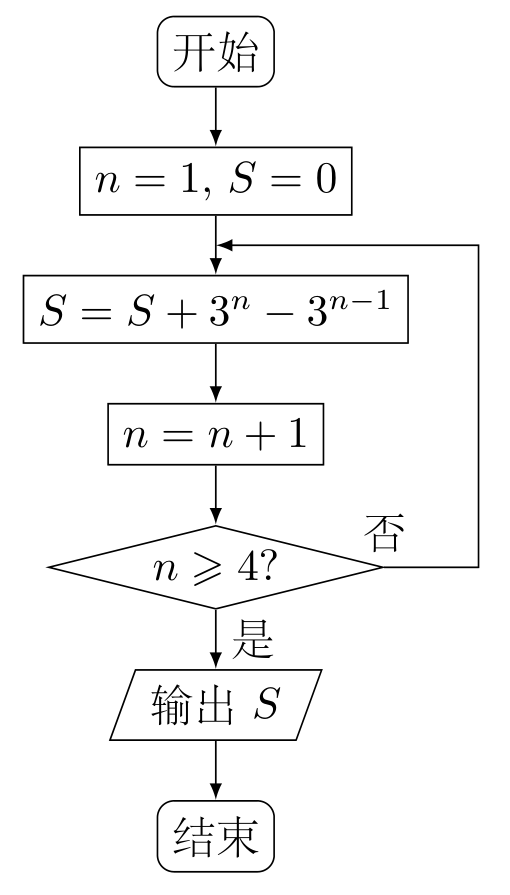
\includegraphics[width=0.82\linewidth]{GaoKao/images/2012/tianjin_liberal/q3_fig1.png}
\end{center}

        {\centering\begin{tabular*}{\linewidth}{@{}@{\extracolsep{\fill}}llll@{}}
          \text{A. }8  &  \text{B. }18  &  \text{C. }26  &  \text{D. }80
        \end{tabular*}\par}

        \item 已知 \(a = 2^{1.2}\)，\(b = \left(\frac{1}{2}\right)^{-0.8}\)，\(c = 2\log_5 2\)，则 \(a\)，\(b\)，\(c\) 的大小关系为（\quad）

        {\centering\begin{tabular*}{\linewidth}{@{}@{\extracolsep{\fill}}llll@{}}
          \text{A. }\(c < b < a\)  &  \text{B. }\(c < a < b\)  &  \text{C. }\(b < a < c\)  &  \text{D. }\(b < c < a\)
        \end{tabular*}\par}

        \item 设 \(x \in \mathbb{R}\)，则“\(x > \frac{1}{2}\)”是“\(2x^2 + x - 1 > 0\)”的（\quad）

        {\centering\begin{tabular*}{\linewidth}{@{}@{\extracolsep{\fill}}llll@{}}
          \text{A. }充分而不必要条件  &  \text{B. }必要而不充分条件  &  \text{C. }充分必要条件  &  \text{D. }既不充分也不必要条件
        \end{tabular*}\par}

        \item 下列函数中，既是偶函数，又在区间 \((1,2)\) 内是增函数的函数为（\quad）

        {\centering\begin{tabular*}{\linewidth}{@{}@{\extracolsep{\fill}}llll@{}}
          \text{A. }\(y = \cos 2x, x \in \mathbb{R}\)  &  \text{B. }\(y = \log_2 |x|\)，\(x \in \mathbb{R}\) 且 \( x \neq 0 \)  &  \text{C. }\(y = \frac{{\mathrm{e}}^x - {\mathrm{e}}^{-x}}{2}\)，\(x \in \mathbb{R}\)  &  \text{D. }\(y = x^{3} + 1\)，\(x \in \mathbb{R}\)
        \end{tabular*}\par}

        \item 将函数 \( f(x) = \sin \omega x \) （其中 \( \omega > 0 \)） 的图象向右平移 \( \frac{\pi}{4} \) 个单位长度，所得图象经过点 \( \left(\frac{3\pi}{4}, 0\right) \)，则 \( \omega \) 的最小值是（\quad）

        {\centering\begin{tabular*}{\linewidth}{@{}@{\extracolsep{\fill}}llll@{}}
          \text{A. }\( \frac{1}{3} \)  &  \text{B. }1  &  \text{C. }\( \frac{5}{3} \)  &  \text{D. }2
        \end{tabular*}\par}

        \item 在 \(\triangle ABC\) 中，\(\angle A = 90^{\circ}\)，\(AB = 1\)，\(AC = 2\). 设点 \(P\)，\(Q\) 满足 \(\overrightarrow{AP} = \lambda \overrightarrow{AB}\)，\(\overrightarrow{AQ} = (1 - \lambda)\overrightarrow{AC}\)，\(\lambda \in \mathbb{R}\). 若 \(\overrightarrow{BQ} \cdot \overrightarrow{CP} = -2\)，则 \(\lambda =\)（\quad）

        {\centering\begin{tabular*}{\linewidth}{@{}@{\extracolsep{\fill}}llll@{}}
          \text{A. }\( \frac{1}{3} \)  &  \text{B. }\( \frac{2}{3} \)  &  \text{C. }\( \frac{4}{3} \)  &  \text{D. }2
        \end{tabular*}\par}

    \end{enumerate}

\end{description}

\begin{description}

    \item[二、填空题]

    \begin{enumerate}[leftmargin=5pt]

      \addtocounter{enumi}{+8}

        \item 集合 \(A = \{x \in \mathbb{R} \mid |x - 2| \leqslant 5\}\) 中的最小整数为\rule[-0.3ex]{3em}{0.4pt}.

        \item 一个几何体的三视图如图所示（单位：\(\mathrm{m}\)），则该几何体的体积为\rule[-0.3ex]{3em}{0.4pt}\(\mathrm{m}^3\).

\begin{center}
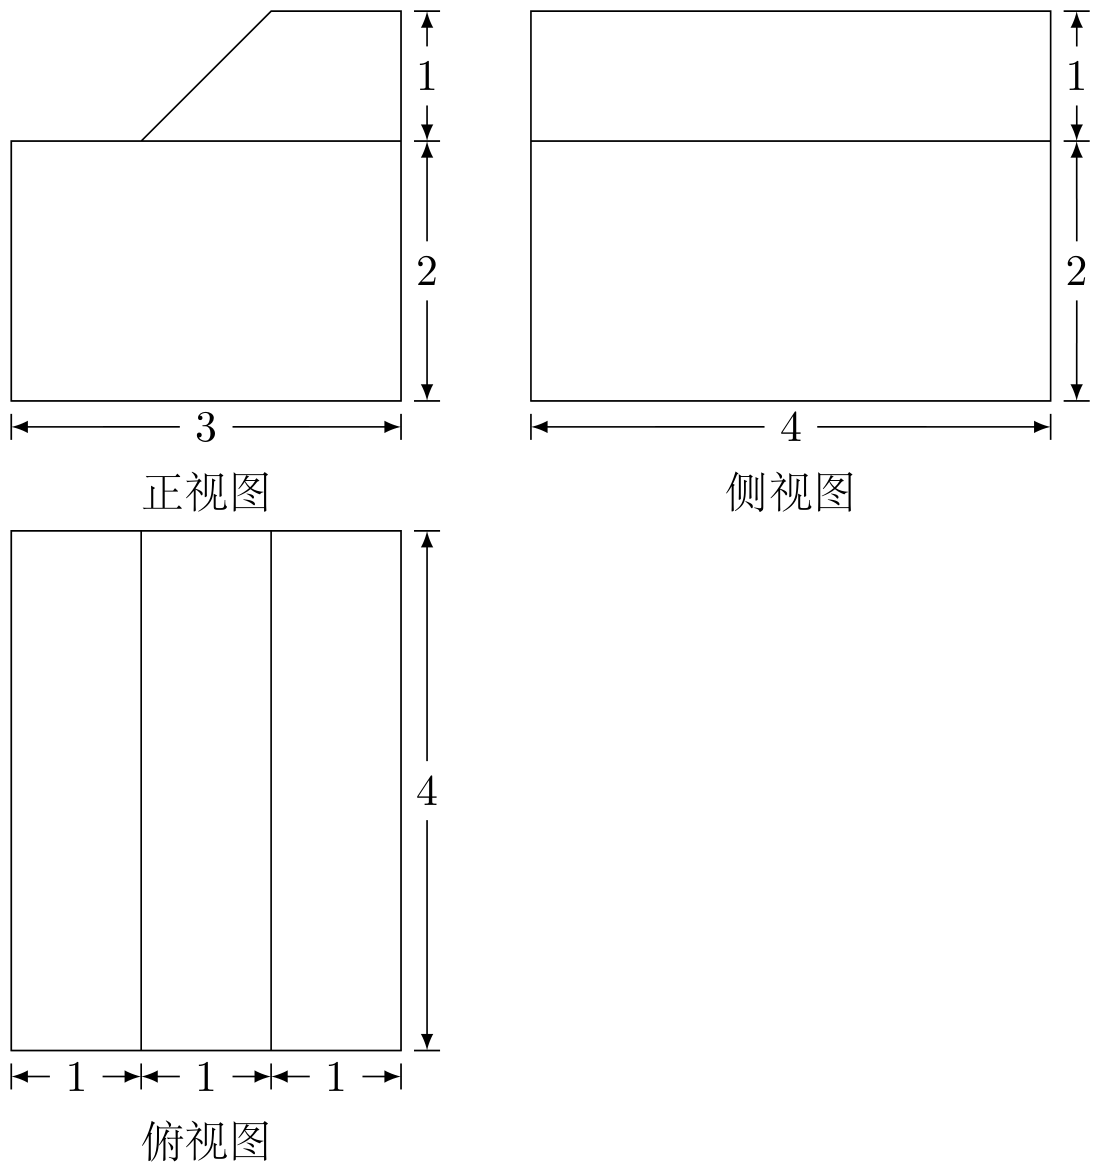
\includegraphics[width=10.8cm]{GaoKao/images/2012/tianjin_liberal/q10_fig1.png}
\end{center}

        \item 已知双曲线 \(C_{1}:\frac{x^{2}}{a^{2}} -\frac{y^{2}}{b^{2}} = 1\) （\(a > 0,b > 0\)）与双曲线 \(C_2:\frac{x^2}{4} -\frac{y^2}{16} = 1\) 有相同的渐近线，且 \(C_1\) 的右焦点为 \(F(\sqrt{5},0)\)，则 \(a =\rule[-0.3ex]{3em}{0.4pt}\)，\(\ b =\rule[-0.3ex]{3em}{0.4pt}\).

        \item 设 \(m\)，\(n \in \mathbb{R}\)，若直线 \(l: mx + ny - 1 = 0\) 与 \(x\) 轴相交于点 \(A\)，与 \(y\) 轴相交于点 \(B\)，且 \(l\) 与圆 \(x^2 + y^2 = 4\) 相交所得弦的长为 \(2\)，\(O\) 为坐标原点，则 \(\triangle AOB\) 面积的最小值为\rule[-0.3ex]{3em}{0.4pt}.

        \item 如图，已知 \(AB\) 和 \(AC\) 是圆的两条弦，过点 \(B\) 作圆的切线与 \(AC\) 的延长线相交于点 \(D\). 过点 \(C\) 作 \(BD\) 的平行线与圆相交于点 \(E\)，与 \(AB\) 相交于点 \(F\)，\(AF = 3\)，\(FB = 1\)，\(EF = \frac{3}{2}\)，则线段 \(CD\) 的长为\rule[-0.3ex]{3em}{0.4pt}.
\begin{center}
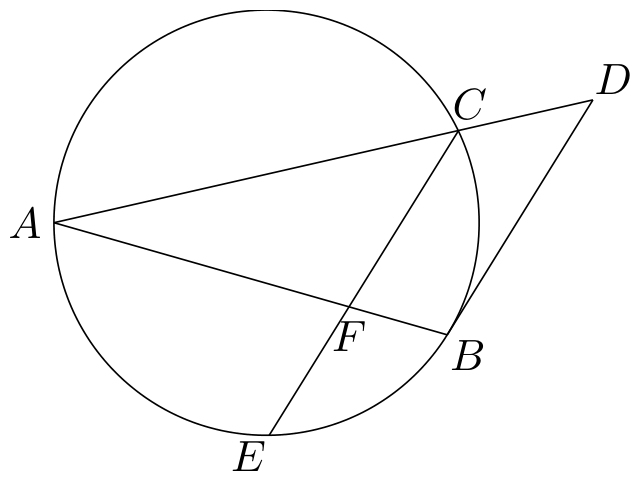
\includegraphics[width=7.9cm]{GaoKao/images/2012/tianjin_liberal/q13_fig1.png}
\end{center}

        \item 已知函数 \( y = \frac{|x^2 - 1|}{x - 1} \) 的图象与函数 \( y = kx \) 的图象恰有两个交点，则实数 \( k \) 的取值范围是\rule[-0.3ex]{3em}{0.4pt}.

    \end{enumerate}

\end{description}

\begin{description}

    \item[三、解答题]

    \begin{enumerate}[leftmargin=5pt]

      \addtocounter{enumi}{+14}

        \item 某地区有小学 \(21\text{ 所}\)，中学 \(14\text{ 所}\)，大学 \(7\text{ 所}\)，现采用分层抽样的方法从这些学校中抽取 \(6\text{ 所}\) 学校对学生进行视力调查.
\begin{enumerate}
\item 求应从小学，中学，大学中分别抽取的学校数目；
\item 若从抽取的 \(6\text{ 所}\) 学校中随机抽取 \(2\text{ 所}\) 学校做进一步数据分析，
\begin{enumerate}
\item 列出所有可能的抽取结果；
\item 求抽取的 \(2\text{ 所}\) 学校均为小学的概率.
\end{enumerate}
\end{enumerate}

        \item 在 \(\triangle ABC\) 中，内角 \(A\)，\(B\)，\(C\) 所对的边分别是 \(a\)，\(b\)，\(c\). 已知 \(a = 2\)，\(c = \sqrt{2}\)，\(\cos A = -\frac{\sqrt{2}}{4}\).
\begin{enumerate}
\item 求 \(\sin C\) 和 \(b\) 的值；
\item 求 \( \cos\left(2A+\frac{\pi}{3}\right) \) 的值.
\end{enumerate}

        \item 如图，在四棱锥 \(P - ABCD\) 中，底面 \(ABCD\) 是矩形，\(AD \perp PD\)，\(BC = 1\)，\(PC = 2\sqrt{3}\)，\(PD = CD = 2\).
\begin{enumerate}
\item 求异面直线 \(PA\) 与 \(BC\) 所成角的正切值；
\item 证明：平面 \(PDC \perp\) 平面 \(ABCD\)；
\item 求直线 \(PB\) 与平面 \(ABCD\) 所成角的正弦值.
\end{enumerate}
\begin{center}
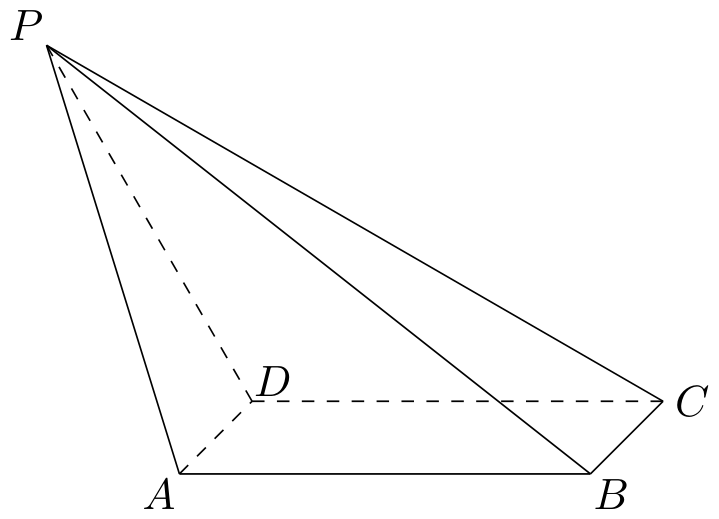
\includegraphics[width=8.4cm]{GaoKao/images/2012/tianjin_liberal/q17_fig1.png}
\end{center}

        \item 已知 \(\{a_{n}\}\) 是等差数列，其前 \(n\) 项和为 \(S_{n}\)，\(\{b_{n}\}\) 是等比数列，且 \(a_{1} = b_{1} = 2\)，\(a_{4} + b_{4} = 27\)，\(S_{4} - b_{4} = 10\).
\begin{enumerate}
\item 求数列 \( \{a_{n}\} \) 与 \( \{b_{n}\} \) 的通项公式；
\item 记 \(T_{n} = a_{1}b_{1} + a_{2}b_{2} + \dots + a_{n}b_{n}\)，\(n \in \mathbf{N}^{*}\)，证明： \(T_{n} - 8 = a_{n-1}b_{n+1}\)（\(n \in \mathbf{N}^{*}\)，\(n > 2\)）.
\end{enumerate}

        \item 已知椭圆 \(\frac{x^2}{a^2} + \frac{y^2}{b^2} = 1\)（\(a > b > 0\)），点 \(P\left(\frac{\sqrt{5}}{5}a, \frac{\sqrt{2}}{2}a\right)\) 在椭圆上.
\begin{enumerate}
\item 求椭圆的离心率；
\item 设 \(A\) 为椭圆的左顶点，\(O\) 为坐标原点. 若点 \(Q\) 在椭圆上且满足 \(|AQ| = |AO|\)，求直线 \(OQ\) 的斜率的值.
\end{enumerate}

        \item 已知函数 \(f(x) = \frac{1}{3} x^3 + \frac{1 - a}{2} x^2 - ax - a\)，\(x \in \mathbb{R}\)，其中 \( a > 0 \).
\begin{enumerate}
\item 求函数 \( f(x) \) 的单调区间；
\item 若函数 \( f(x) \) 在区间 \((-2,0)\) 内恰有两个零点，求 \( a \) 的取值范围；
\item 当 \(a = 1\) 时，设函数 \(f(x)\) 在区间 \([t, t + 3]\) 上的最大值为 \(M(t)\)，最小值为 \(m(t)\)，记 \(g(t) = M(t) - m(t)\)，求函数 \(g(t)\) 在区间 \([-3, -1]\) 上的最小值.
\end{enumerate}

    \end{enumerate}

\end{description}


\subsection{2012年浙江卷（理）}\label{gk:2012年浙江卷（理）}

\begin{description}

    \item[一、选择题]

    \begin{enumerate}[leftmargin=5pt]

        \item 设集合 \(A = \{x \mid 1 < x < 4\}\)，集合 \(B = \{x \mid x^2 - 2x - 3 \leqslant 0\}\)，则 \(A \cap (\complement_{\mathbb{R}} B) =\)（\quad）

        {\centering\begin{tabular*}{\linewidth}{@{}@{\extracolsep{\fill}}llll@{}}
          \text{A. }\((1, 4)\)  &  \text{B. }\((3, 4)\)  &  \text{C. }\((1, 3)\)  &  \text{D. }\((1,2)\) \(\cup\) \((3,4)\)
        \end{tabular*}\par}

        \item 已知 \(\i\) 是虚数单位，则 \( \frac{3+\i}{1-\i}= \)（\quad）

        {\centering\begin{tabular*}{\linewidth}{@{}@{\extracolsep{\fill}}llll@{}}
          \text{A. }\(1-2\i\)  &  \text{B. }\(2-\i\)  &  \text{C. }\(2 + \i\)  &  \text{D. }\(1 + 2\i\)
        \end{tabular*}\par}

        \item 设 \(a \in \mathbb{R}\)，则“\(a = 1\)”是直线 \(l_1: ax + 2y - 1 = 0\) 与直线 \(l_2: x + (a + 1)y + 4 = 0\) 平行的（\quad）

        {\centering\begin{tabular*}{\linewidth}{@{}@{\extracolsep{\fill}}llll@{}}
          \text{A. }充分不必要条件  &  \text{B. }必要不充分条件  &  \text{C. }充分必要条件  &  \text{D. }既不充分也不必要条件
        \end{tabular*}\par}

        \item 把函数 \( y = \cos 2x + 1 \) 的图象上所有点的横坐标伸长到原来的 \(2\) 倍（纵坐标不变），然后向左平移 \(1\) 个单位长度，再向下平移 \(1\) 个单位长度，得到的图象是 （\quad）

        {\centering\begin{tabular*}{\linewidth}{@{}@{\extracolsep{\fill}}cccc@{}}
          \text{A. }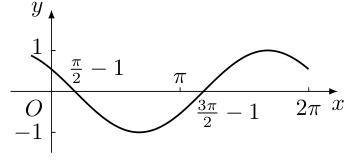
\includegraphics[width=0.15\paperwidth]{GaoKao/images/2012/zhejiang_science/q4_optA.png}  &  \text{B. }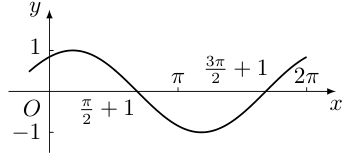
\includegraphics[width=0.15\paperwidth]{GaoKao/images/2012/zhejiang_science/q4_optB.png}  &  \text{C. }\includegraphics[width=0.15\paperwidth]{GaoKao/images/2012/zhejiang_science/q4_optC.png}  &  \text{D. }\includegraphics[width=0.15\paperwidth]{GaoKao/images/2012/zhejiang_science/q4_optD.png}
        \end{tabular*}\par}

        \item 设 \(\bm{a}\)，\(\bm{b}\) 是两个非零向量（\quad）

        {\centering\begin{tabular*}{\linewidth}{@{}@{\extracolsep{\fill}}llll@{}}
          \text{A. }若 \(|\bm{a} + \bm{b}| = |\bm{a}| - |\bm{b}|\)，则 \(\bm{a} \perp \bm{b}\)  &  \text{B. }若 \(\bm{a} \perp \bm{b}\)，则 \(|\bm{a} + \bm{b}| = |\bm{a}| - |\bm{b}|\)  &  \text{C. }若 \(|\bm{a} + \bm{b}| = |\bm{a}| - |\bm{b}|\)，则存在实数 \(\lambda\)，使得 \(\bm{b} = \lambda \bm{a}\)  &  \text{D. }若存在实数 \(\lambda\)，使得 \(\bm{b} = \lambda \bm{a}\)，则 \(|\bm{a} + \bm{b}| = |\bm{a}| - |\bm{b}|\)
        \end{tabular*}\par}

        \item 若从 \(1\)，\(2\)，\(3\)，\(\cdots\)，\(9\) 这 9 个整数中同时取 4 个不同的数，其和为偶数，则不同的取法共有（\quad）

        {\centering\begin{tabular*}{\linewidth}{@{}@{\extracolsep{\fill}}llll@{}}
          \text{A. }\(60\text{ 种}\)  &  \text{B. }\(63\text{ 种}\)  &  \text{C. }\(65\text{ 种}\)  &  \text{D. }\(66\text{ 种}\)
        \end{tabular*}\par}

        \item 设 \(S_{n}\) 是公差为 \(d\)（\(d \neq 0\)） 的无穷等差数列 \(\{a_{n}\}\) 的前 \(n\) 项和，则下列命题错误的是（\quad）

        {\centering\begin{tabular*}{\linewidth}{@{}@{\extracolsep{\fill}}llll@{}}
          \text{A. }若 \(d < 0\)，则数列 \(\{S_{n}\}\) 有最大项  &  \text{B. }若数列 \(\{S_{n}\}\) 有最大项，则 \(d < 0\)  &  \text{C. }若数列 \(\{S_{n}\}\) 是递增数列，则对任意 \(n \in \mathbf{N}^{*}\)，均有 \(S_{n} > 0\)  &  \text{D. }若对任意 \(n \in \mathbf{N}^{*}\)，均有 \(S_n > 0\)，则数列 \(\{S_n\}\) 是递增数列
        \end{tabular*}\par}

        \item 如图，\(F_{1}\)，\(F_{2}\) 分别是双曲线 \(C: \frac{x^{2}}{a^{2}} - \frac{y^{2}}{b^{2}} = 1 \) （\(a, b > 0\)）的左，右焦点，\(B\) 是虚轴的端点，直线 \(F_{1}B\) 与 \(C\) 的两条渐近线分别交于 \(P\)，\(Q\) 两点，线段 \(PQ\) 的垂直平分线与 \(x\) 轴交于点 \(M\). 若 \(|MF_{2}| = |F_{1}F_{2}|\)，则 \(C\) 的离心率是（\quad）

        {\centering\begin{tabular*}{\linewidth}{@{}@{\extracolsep{\fill}}llll@{}}
          \text{A. }\(\frac{2\sqrt{3}}{3}\)  &  \text{B. }\(\frac{\sqrt{6}}{2}\)  &  \text{C. }\(\sqrt{2}\)  &  \text{D. }\(\sqrt{3}\)
        \end{tabular*}\par}

        \item 设 \(a > 0\)，\(b > 0\).（\quad）

        {\centering\begin{tabular*}{\linewidth}{@{}@{\extracolsep{\fill}}llll@{}}
          \text{A. }若 \(2^{a} + 2a = 2^{b} + 3b\)，则 \(a > b\)  &  \text{B. }若 \(2^{a} + 2a = 2^{b} + 3b\)，则 \(a < b\)  &  \text{C. }若 \(2^{a} - 2a = 2^{b} - 3b\)，则 \(a > b\)  &  \text{D. }若 \(2^{a} - 2a = 2^{b} - 3b\)，则 \(a < b\)
        \end{tabular*}\par}

        \item 已知矩形 \(ABCD\)，\(AB = 1\)，\(BC = \sqrt{2}\)，将 \(\triangle ABD\) 沿矩形的对角线 \(BD\) 所在的直线进行翻折，在翻折过程中（\quad）

        {\centering\begin{tabular*}{\linewidth}{@{}@{\extracolsep{\fill}}llll@{}}
          \text{A. }存在某个位置，使得直线 \(AC\) 与直线 \(BD\) 垂直  &  \text{B. }存在某个位置，使得直线 \(AB\) 与直线 \(CD\) 垂直  &  \text{C. }存在某个位置，使得直线 \(AD\) 与直线 \(BC\) 垂直  &  \text{D. }对任意位置，三对直线“\(AC\) 与 \(BD\)”，“\(AB\) 与 \(CD\)”，“\(AD\) 与 \(BC\)”均不垂直
        \end{tabular*}\par}

    \end{enumerate}

\end{description}

\begin{description}

    \item[二、填空题]

    \begin{enumerate}[leftmargin=5pt]

      \addtocounter{enumi}{+10}

        \item 已知某三棱锥的三视图（单位：\(\mathrm{cm}\)）如图所示，则该三棱锥的体积等于\rule[-0.3ex]{3em}{0.4pt} \(\mathrm{cm}^3\).

\begin{center}
\includegraphics[width=8.6cm]{GaoKao/images/2012/zhejiang_science/q11_fig1.png}
\end{center}

        \item 若某程序框图如图所示，则该程序运行后输出的值是\rule[-0.3ex]{3em}{0.4pt}.

\begin{center}
\begin{center}
\includegraphics[width=0.42\linewidth]{GaoKao/images/2012/zhejiang_science/q12_fig1.png}
\end{center}
\end{center}

        \item 设公比为 \(q\)（\(q>0\)）的等比数列 \(\{a_{n}\}\) 的前 \(n\) 项和为 \(S_{n}\). 若 \(S_{2} = 3a_{2} + 2\)，\(S_{4} = 3a_{4} + 2\)，则 \(q =\rule[-0.3ex]{3em}{0.4pt}\).

        \item 若将函数 \( f(x) = x^5 \) 表示为 \( f(x) = a_0 + a_1(1 + x) + a_2(1 + x)^2 + \cdots + a_5(1 + x)^5 \)，其中 \(a_0\)，\(a_1\)，\(a_2\)，\(\cdots\)，\(a_5\) 为实数，则 \( a_3 = \)\rule[-0.3ex]{3em}{0.4pt}.

        \item 在 \(\triangle ABC\) 中，\(M\) 是 \(BC\) 的中点，\(AM = 3\)，\(BC = 10\). 则 \(\overrightarrow{AB} \cdot \overrightarrow{AC} =\)\rule[-0.3ex]{3em}{0.4pt}.

        \item 定义：曲线 \(C\) 上的点到直线 \(l\) 的距离的最小值为曲线 \(C\) 到直线 \(l\) 的距离. 已知曲线 \( C_{1}: y = x^{2} + a \) 到直线 \(l: y = x\) 的距离等于曲线 \( C_{2}: x^{2} + (y + 4)^{2} = 2 \) 到直线 \(l: y = x\) 的距离，则实数 \( a = \)\rule[-0.3ex]{3em}{0.4pt}.

        \item 设 \(a \in \mathbb{R}\)，若 \(x > 0\) 时均有 \([(a - 1)x - 1](x^2 - ax - 1) \geqslant 0\)，则 \(a = \)\rule[-0.3ex]{3em}{0.4pt}.

    \end{enumerate}

\end{description}

\begin{description}

    \item[三、解答题]

    \begin{enumerate}[leftmargin=5pt]

      \addtocounter{enumi}{+17}

        \item 在 \(\triangle ABC\) 中，内角 \(A\)，\(B\)，\(C\) 的对边分别为 \(a\)，\(b\)，\(c\). 已知 \(\cos A = \frac{2}{3}\)，\(\sin B = \sqrt{5} \cos C\).
\begin{enumerate}
\item 求 \(\tan C\) 的值；
\item 若 \(a = \sqrt{2}\)，求 \(\triangle ABC\) 的面积.
\end{enumerate}

        \item 已知箱中装有 \(4\) 个白球和 \(5\) 个黑球，且规定：取出一个白球得 \(2\) 分，取出一个黑球得 \(1\) 分. 现从该箱中任取（无放回，且每球取到的机会均等） \(3\) 个球，记随机变量 \(X\) 为取出此 \(3\) 个球所得分数之和.
\begin{enumerate}
\item 求 \(X\) 的分布列；
\item 求 \(E(X)\).
\end{enumerate}

        \item 如图，在四棱锥 \(P - ABCD\) 中，底面是边长为 \(2\sqrt{3}\) 的菱形，\(\angle BAD = 120^{\circ}\)，且 \(PA \perp\) 平面 \(ABCD\)，\(PA = 2\sqrt{6}\)，\(M\)，\(N\) 分别为 \(PB\)，\(PD\) 的中点.
\begin{enumerate}
\item 证明： \(MN \parallel\) 平面 \(ABCD\)；
\item 过点 \(A\) 作 \(AQ \perp PC\)，垂足为点 \(Q\)，求二面角 \(A - MN - Q\) 的平面角的余弦值.
\end{enumerate}
\begin{center}
\includegraphics[width=6.6cm]{GaoKao/images/2012/zhejiang_science/q20_fig1.png}
\end{center}

        \item 如图，椭圆 \(C: \frac{x^2}{a^2} + \frac{y^2}{b^2} = 1 \) （\(a > b > 0\)）的离心率为 \(\frac{1}{2}\). 其左焦点到点 \(P(2,1)\) 的距离为 \(\sqrt{10}\). 不经过原点 \(O\) 的直线 \(l\) 与 \(C\) 相交于 \(A\)，\(B\) 两点，且线段 \(AB\) 被直线 \(OP\) 平分.
\begin{enumerate}
\item 求椭圆 \(C\) 的方程；
\item 求 \( \triangle ABP \) 面积取最大值时直线 \(l\) 的方程.
\end{enumerate}
\begin{center}
\includegraphics[width=9.0cm]{GaoKao/images/2012/zhejiang_science/q21_fig1.png}
\end{center}

        \item 已知 \(a > 0\)，\(b \in \mathbb{R}\)，函数 \(f(x) = 4ax^3 - 2bx - a + b\).
\begin{enumerate}
\item 证明：当 \(0 \leqslant x \leqslant 1\) 时，
\begin{enumerate}
\item 函数 \(f(x)\) 的最大值为 \(|2a-b|+a\)；
\item \(f(x)+|2a-b|+a\geqslant0\)；
\end{enumerate}
\item 若 \(-1 \leqslant f(x) \leqslant 1\) 对 \(x \in [0,1]\) 恒成立，求 \(a+b\) 的取值范围.
\end{enumerate}

    \end{enumerate}

\end{description}


\subsection{2012年浙江卷（文）}\label{gk:2012年浙江卷（文）}

\begin{description}

    \item[一、选择题]

    \begin{enumerate}[leftmargin=5pt]

        \item 设全集 \(U = \{1, 2, 3, 4, 5, 6\}\)，集合 \(P = \{1, 2, 3, 4\}\)，\(Q = \{3, 4, 5\}\)，则 \(P \cap (\complement_U Q) =\)（\quad）

        {\centering\begin{tabular*}{\linewidth}{@{}@{\extracolsep{\fill}}llll@{}}
          \text{A. }\(\{1, 2, 3, 4, 6\}\)  &  \text{B. }\(\{1,2,3,4,5\}\)  &  \text{C. }\(\{1,2,5\}\)  &  \text{D. }\(\{1,2\}\)
        \end{tabular*}\par}

        \item 已知 \(\i\) 是虚数单位，则 \( \frac{3+\i}{1-\i}= \)（\quad）

        {\centering\begin{tabular*}{\linewidth}{@{}@{\extracolsep{\fill}}llll@{}}
          \text{A. }\(1 - 2\i\)  &  \text{B. }\(2 - \i\)  &  \text{C. }\(2 + \i\)  &  \text{D. }\(1 + 2\i\)
        \end{tabular*}\par}

        \item 已知某三棱锥的三视图（单位：\(\mathrm{cm}\)）如图所示，则该三棱锥的体积是（\quad）

\begin{center}
\includegraphics[width=4.5cm]{GaoKao/images/2012/zhejiang_liberal/q3_fig1.png}
\end{center}

        {\centering\begin{tabular*}{\linewidth}{@{}@{\extracolsep{\fill}}llll@{}}
          \text{A. }\(1 \mathrm{~cm}^{3}\)  &  \text{B. }\(2 \mathrm{~cm}^{3}\)  &  \text{C. }\(3 \mathrm{~cm}^{3}\)  &  \text{D. }\(6 \mathrm{~cm}^{3}\)
        \end{tabular*}\par}

        \item 设 \(l\) 是直线，\(\alpha\)，\(\beta\) 是两个不同的平面，下列选项正确的是（\quad）

        {\centering\begin{tabular*}{\linewidth}{@{}@{\extracolsep{\fill}}llll@{}}
          \text{A. }若 \(l \parallel \alpha\)，\(l \parallel \beta\)，则 \(\alpha \parallel \beta\)  &  \text{B. }若 \(l \parallel \alpha\)，\(l \perp \beta\)，则 \(\alpha \perp \beta\)  &  \text{C. }若 \(\alpha \perp \beta\)，\(l \perp \alpha\)，则 \(l \perp \beta\)  &  \text{D. }若 \(\alpha \perp \beta\)，\(l \parallel \alpha\)，则 \(l \perp \beta\)
        \end{tabular*}\par}

        \item 设 \(a \in \mathbb{R}\)，则 \(a = 1\) 是“直线 \(l_1\)：\(ax + 2y - 1 = 0\) 与直线 \(l_2\)：\(x + 2y + 4 = 0\) 平行”的（\quad）

        {\centering\begin{tabular*}{\linewidth}{@{}@{\extracolsep{\fill}}llll@{}}
          \text{A. }充分不必要条件  &  \text{B. }必要不充分条件  &  \text{C. }充分必要条件  &  \text{D. }既不充分也不必要条件
        \end{tabular*}\par}

        \item 把函数 \(y = \cos 2x + 1\) 的图象上所有点的横坐标伸长到原来的 \(2\) 倍（纵坐标不变），然后向左平移 \(1\) 个单位长度，再向下平移 \(1\) 个单位长度，得到的图象是（\quad）

        {\centering\begin{tabular*}{\linewidth}{@{}@{\extracolsep{\fill}}cccc@{}}
          \text{A. }\includegraphics[width=0.15\paperwidth]{GaoKao/images/2012/zhejiang_liberal/q6_A.png}  &  \text{B. }\includegraphics[width=0.15\paperwidth]{GaoKao/images/2012/zhejiang_liberal/q6_B.png}  &  \text{C. }\includegraphics[width=0.15\paperwidth]{GaoKao/images/2012/zhejiang_liberal/q6_C.png}  &  \text{D. }\includegraphics[width=0.15\paperwidth]{GaoKao/images/2012/zhejiang_liberal/q6_D.png}
        \end{tabular*}\par}

        \item 设 \(\bm{a}\)，\(\bm{b}\) 是两个非零向量（\quad）

        {\centering\begin{tabular*}{\linewidth}{@{}@{\extracolsep{\fill}}llll@{}}
          \text{A. }若 \(|\bm{a} + \bm{b}| = |\bm{a}| - |\bm{b}|\)，则 \(\bm{a} \perp \bm{b}\)  &  \text{B. }若 \(\bm{a} \perp \bm{b}\)，则 \(|\bm{a} + \bm{b}| = |\bm{a}| - |\bm{b}|\)  &  \text{C. }若 \(|\bm{a} + \bm{b}| = |\bm{a}| - |\bm{b}|\)，则存在实数 \(\lambda\)，使得 \(\bm{b} = \lambda \bm{a}\)  &  \text{D. }若存在实数 \(\lambda\)，使得 \(\bm{b} = \lambda \bm{a}\)，则 \(|\bm{a} + \bm{b}| = |\bm{a}| - |\bm{b}|\)
        \end{tabular*}\par}

        \item 如图，中心均为原点 \(O\) 的双曲线与椭圆有公共焦点，\(M\)、\(N\) 是双曲线的两顶点. 若 \(M\)、\(O\)、\(N\) 将椭圆长轴四等分，则双曲线与椭圆的离心率的比值是（\quad）

\begin{center}
\includegraphics[width=7.4cm]{GaoKao/images/2012/zhejiang_liberal/q8_fig1.png}
\end{center}

        {\centering\begin{tabular*}{\linewidth}{@{}@{\extracolsep{\fill}}llll@{}}
          \text{A. }3  &  \text{B. }2  &  \text{C. }\(\sqrt{3}\)  &  \text{D. }\(\sqrt{2}\)
        \end{tabular*}\par}

        \item 若正数 \(x\)，\(y\) 满足 \(x + 3y = 5xy\)，则 \(3x + 4y\) 的最小值是（\quad）

        {\centering\begin{tabular*}{\linewidth}{@{}@{\extracolsep{\fill}}llll@{}}
          \text{A. }\( \frac{24}{5} \)  &  \text{B. }\( \frac{28}{5} \)  &  \text{C. }5  &  \text{D. }6
        \end{tabular*}\par}

        \item 设 \(a > 0\)，\(b > 0\)，\({\mathrm{e}}\) 是自然对数的底数（\quad）

        {\centering\begin{tabular*}{\linewidth}{@{}@{\extracolsep{\fill}}llll@{}}
          \text{A. }若 \({\mathrm{e}}^a + 2a = {\mathrm{e}}^b + 3b\)，则 \(a > b\)  &  \text{B. }若 \({\mathrm{e}}^a + 2a = {\mathrm{e}}^b + 3b\)，则 \(a < b\)  &  \text{C. }若 \({\mathrm{e}}^a - 2a = {\mathrm{e}}^b - 3b\)，则 \(a > b\)  &  \text{D. }若 \({\mathrm{e}}^a - 2a = {\mathrm{e}}^b - 3b\)，则 \(a < b\)
        \end{tabular*}\par}

    \end{enumerate}

\end{description}

\begin{description}

    \item[二、填空题]

    \begin{enumerate}[leftmargin=5pt]

      \addtocounter{enumi}{+10}

        \item 某个年级有男生 560 人，女生 420 人，用分层抽样的方法从该年级全体学生中抽取一个容量为 280 的样本，则此样本中男生人数为\rule[-0.3ex]{3em}{0.4pt}.

        \item 从边长为 \(1\) 的正方形的中心和顶点这五点中，随机（等可能）取两点，则该两点间的距离为 \(\frac{\sqrt{2}}{2}\) 的概率是\rule[-0.3ex]{3em}{0.4pt}.

        \item 若某程序框图如图所示，则该程序运行后输出的值是\rule[-0.3ex]{3em}{0.4pt}.

\begin{center}
\includegraphics[width=0.42\linewidth]{GaoKao/images/2012/zhejiang_liberal/q13_fig1.png}
\end{center}

        \item 设 \(z = x + 2y\)，其中实数 \(x\)，\(y\) 满足 \(\begin{cases}
x - y + 1 \geqslant 0,\\
x + y - 2 \leqslant 0,\\
x \geqslant 0,\\
y \geqslant 0,
\end{cases}\) 则 \(z\) 的取值范围是\rule[-0.3ex]{3em}{0.4pt}.

        \item 在 \(\triangle ABC\) 中，\(M\) 是 \(BC\) 的中点，\(AM = 3\)，\(BC = 10\)，则 \(\overrightarrow{AB} \cdot \overrightarrow{AC} = \)\rule[-0.3ex]{3em}{0.4pt}.

        \item 设函数 \( f(x) \) 是定义在 \( \mathbb{R} \) 上的周期为 2 的偶函数，当 \( x \in [0,1] \) 时，\( f(x) = x + 1 \)，则 \( f\left(\frac{3}{2}\right) = \)\rule[-0.3ex]{3em}{0.4pt}.

        \item 定义：曲线 \(C\) 上的点到直线 \(l\) 的距离的最小值称为曲线 \(C\) 到直线 \(l\) 的距离. 已知曲线 \(C_1\)：\(y = x^{2} + a\) 到直线 \(l\)：\(y = x\) 的距离等于曲线 \(C_2\)：\(x^{2} + (y + 4)^{2} = 2\) 到直线 \(l\)：\(y = x\) 的距离，则实数 \(a =\rule[-0.3ex]{3em}{0.4pt}\).

    \end{enumerate}

\end{description}

\begin{description}

    \item[三、解答题]

    \begin{enumerate}[leftmargin=5pt]

      \addtocounter{enumi}{+17}

        \item 在 \(\triangle ABC\) 中，内角 \(A\)，\(B\)，\(C\) 的对边分别为 \(a\)，\(b\)，\(c\)，且 \(b \sin A = \sqrt{3} a \cos B\).

\begin{enumerate}
\item 求角 \(B\) 的大小；
\item 若 \(b = 3\)，\( \sin C = 2 \sin A \)，求 \(a\)，\(c\) 的值.
\end{enumerate}

        \item 已知数列 \(\{a_{n}\}\) 的前 \(n\) 项和为 \(S_{n}\)，且 \(S_{n} = 2n^{2} + n\)，\(n \in \mathbf{N}^{*}\)，数列 \(\{b_{n}\}\) 满足 \(a_{n} = 4\log_{2}b_{n} + 3\)，\(n \in \mathbf{N}^{*}\).

\begin{enumerate}
\item 求 \(a_{n}\)，\(b_{n}\)；
\item 求数列 \(\{a_{n} \cdot b_{n}\}\) 的前 \(n\) 项和 \(T_{n}\).
\end{enumerate}

        \item 如图，在侧棱垂直底面的四棱柱 \(ABCD - A_{1}B_{1}C_{1}D_{1}\) 中，\(AD \parallel BC\)，\(AD \perp AB\)，\(AB = \sqrt{2}\)，\(AD = 2\)，\(BC = 4\)，\(AA_{1} = 2\)，\(E\) 是 \(DD_{1}\) 的中点，\(F\) 是平面 \(B_{1}C_{1}E\) 与直线 \(AA_{1}\) 的交点.

\begin{enumerate}
    \item 证明：
    \begin{enumerate}
    \item \(EF \parallel A_{1}D_{1}\)；
\item \(BA_{1} \perp\) 平面 \(B_{1}C_{1}EF\).
\end{enumerate}
\item 求 \(BC_{1}\) 与平面 \(B_{1}C_{1}EF\) 所成的角的正弦值.
\end{enumerate}

\begin{center}
\includegraphics[width=7.5cm]{GaoKao/images/2012/zhejiang_liberal/q20_fig1.png}
\end{center}

        \item 已知 \(a \in \mathbb{R}\)，函数 \(f(x) = 4x^3 - 2ax + a\).

\begin{enumerate}
\item 求 \(f(x)\) 的单调区间；
\item 证明：当 \(0 \leqslant x \leqslant 1\) 时，\(f(x) + |2 - a| > 0\).
\end{enumerate}

        \item 如图，在直角坐标系 \(xOy\) 中，点 \(P\left(1, \frac{1}{2}\right)\) 到抛物线 \(C: y^2 = 2px \) （\(p > 0\)）的准线的距离为 \(\frac{5}{4}\). 点 \(M(t, 1)\) 是 \(C\) 上的定点，\(A\)，\(B\) 是 \(C\) 上的两动点，且线段 \(AB\) 被直线 \(OM\) 平分.

\begin{enumerate}
\item 求 \(p\)，\(t\) 的值；
\item 求 \(\triangle ABP\) 面积的最大值.
\end{enumerate}

\begin{center}
\includegraphics[width=7.7cm]{GaoKao/images/2012/zhejiang_liberal/q22_fig1.png}
\end{center}

    \end{enumerate}

\end{description}
